\documentclass[10pt, letterpaper]{article}

\usepackage{setspace}
\usepackage[letterpaper, margin=1.0in]{geometry}
\usepackage{amsmath}   % includes \boldmath(), \boldsymbol{()}
\usepackage{bm}        % math fonts, \boldmath{}, \boldsymbol{}
\usepackage[authoryear, round, semicolon]{natbib}
\usepackage{graphicx}
\bibliographystyle{plainnat}
%\usepackage[style=apa, citestyle=authoryear, language=american]{biblatex}
%\DeclareLanguageMapping{american}{american-apa}
%\addbibresource{XTXBibliography.bib}
%\bibliographystyle{plain}
%\renewcommand\multicitedelim{\addsemicolon\space}
\usepackage{graphicx}
\graphicspath{ {Images/} }
\usepackage{float}
\usepackage{caption}
%\captionsetup[table]{skip=10pt, belowskip=12pt}
\providecommand{\keywords}[1]{\noindent\textbf{Keywords:  } #1}
\usepackage{subcaption}
\newcommand{\mt}[1]{\bm{#1}^{\prime}}
\newcommand{\mtm}[2]{\bm{#1}^{\prime}\bm{#2}}
\newcommand{\mi}[1]{\bm{#1}^{-1}}
\newcommand{\mest}[1]{\hat{\bm{#1}}}
\usepackage[bottom]{footmisc}
\setlength{\skip\footins}{12pt}
\setlength\parindent{0pt}

\title{\Large A Framework for Sharing Confidential Research Data, Applied to Investigating Differential Pay by Race in the U. S. Government\\
\vspace{12pt} \Large Supplement:  Synthetic Data Validation}

\author{Duke University Synthetic Data Project}

\begin{document}

\begin{spacing}{1.0}

\maketitle

\vspace{20pt}

The following graphs and tables are excerpted from work done by the Synthetic Data Team at Duke University to validate the DIBBS synthetic federal employee data set with corresponding authentic data supplied by the U.S. Office of Personnel Management (OPM).\footnote{A complete description of both data sets and sources is available in the main document that the current document supplements.}  The selection here highlights two and three level covariate relationships, especially involving important research variables such as sex, race, age, education, agency, occupation, year, and pay.  In assessing similarity of the data sets, emphasis is placed on utility, or the degree to which answers to meaningful research questions obtained from use of synthetic data agree with those from use of corresponding authentic data.  Graphs and tables representing synthetic data contain the text ``DIBBS" while those for authentic data contain either ``OPM" or ``JdF."\footnote{``JdF" is nomenclature for a particular FOIA request that resulted in receipt of authentic data from OPM, which was used to generate synthetic data.}  All codes and definitions are taken from the U.S. Office of Personnel Management Guide to Data Standards \citep{OPMGDS}.  For additional information and guidance on use and interpretation of data made available by OPM, see \citep{OPMDataAnalysisDocumentation}.\\

\vspace{0.5in}

TWO VARIABLE CORRELATION\\

Figure \ref{figure:JdFDIBBSCorrelation} shows, for pay plan GS, full-time observations, correlations between 1.) the variable indicated in the title bars and 2.) all levels of all other variables in title bars.  Synthetic variable pair correlations are plotted (y-axis) against corresponding pair correlations in the authentic data (x-axis).  Points lying near the reference line (slope of 1.0) indicate equality between data sets.  Agency and occupation are truncated to the first two positions.  Note that correlations involving categorical variables, or fixed effects, effectively measure the association of proportion of observations with levels of the second variable.  Missing counts are the number of variable level combinations that appear in the other data set but not in the one indicating a count.  For instance, JdF=2 in the agency panel would indicate that observations exist in the synthetic data, but not in the authentic data, for two combinations of agency and some level of a second variable.  Note that all missing counts are a multiple of three.  This is due to agencies AL, CP, and GD missing in the synthetic data.\\

Observation:  Correlation of pairs of levels of variables within synthetic data are very near those of  corresponding pairs in the authentic data. This is indicated by the near proximity of all plotted points to the reference line of slope 1.0, including those for extreme correlation values.  

\begin{figure}[ht]
    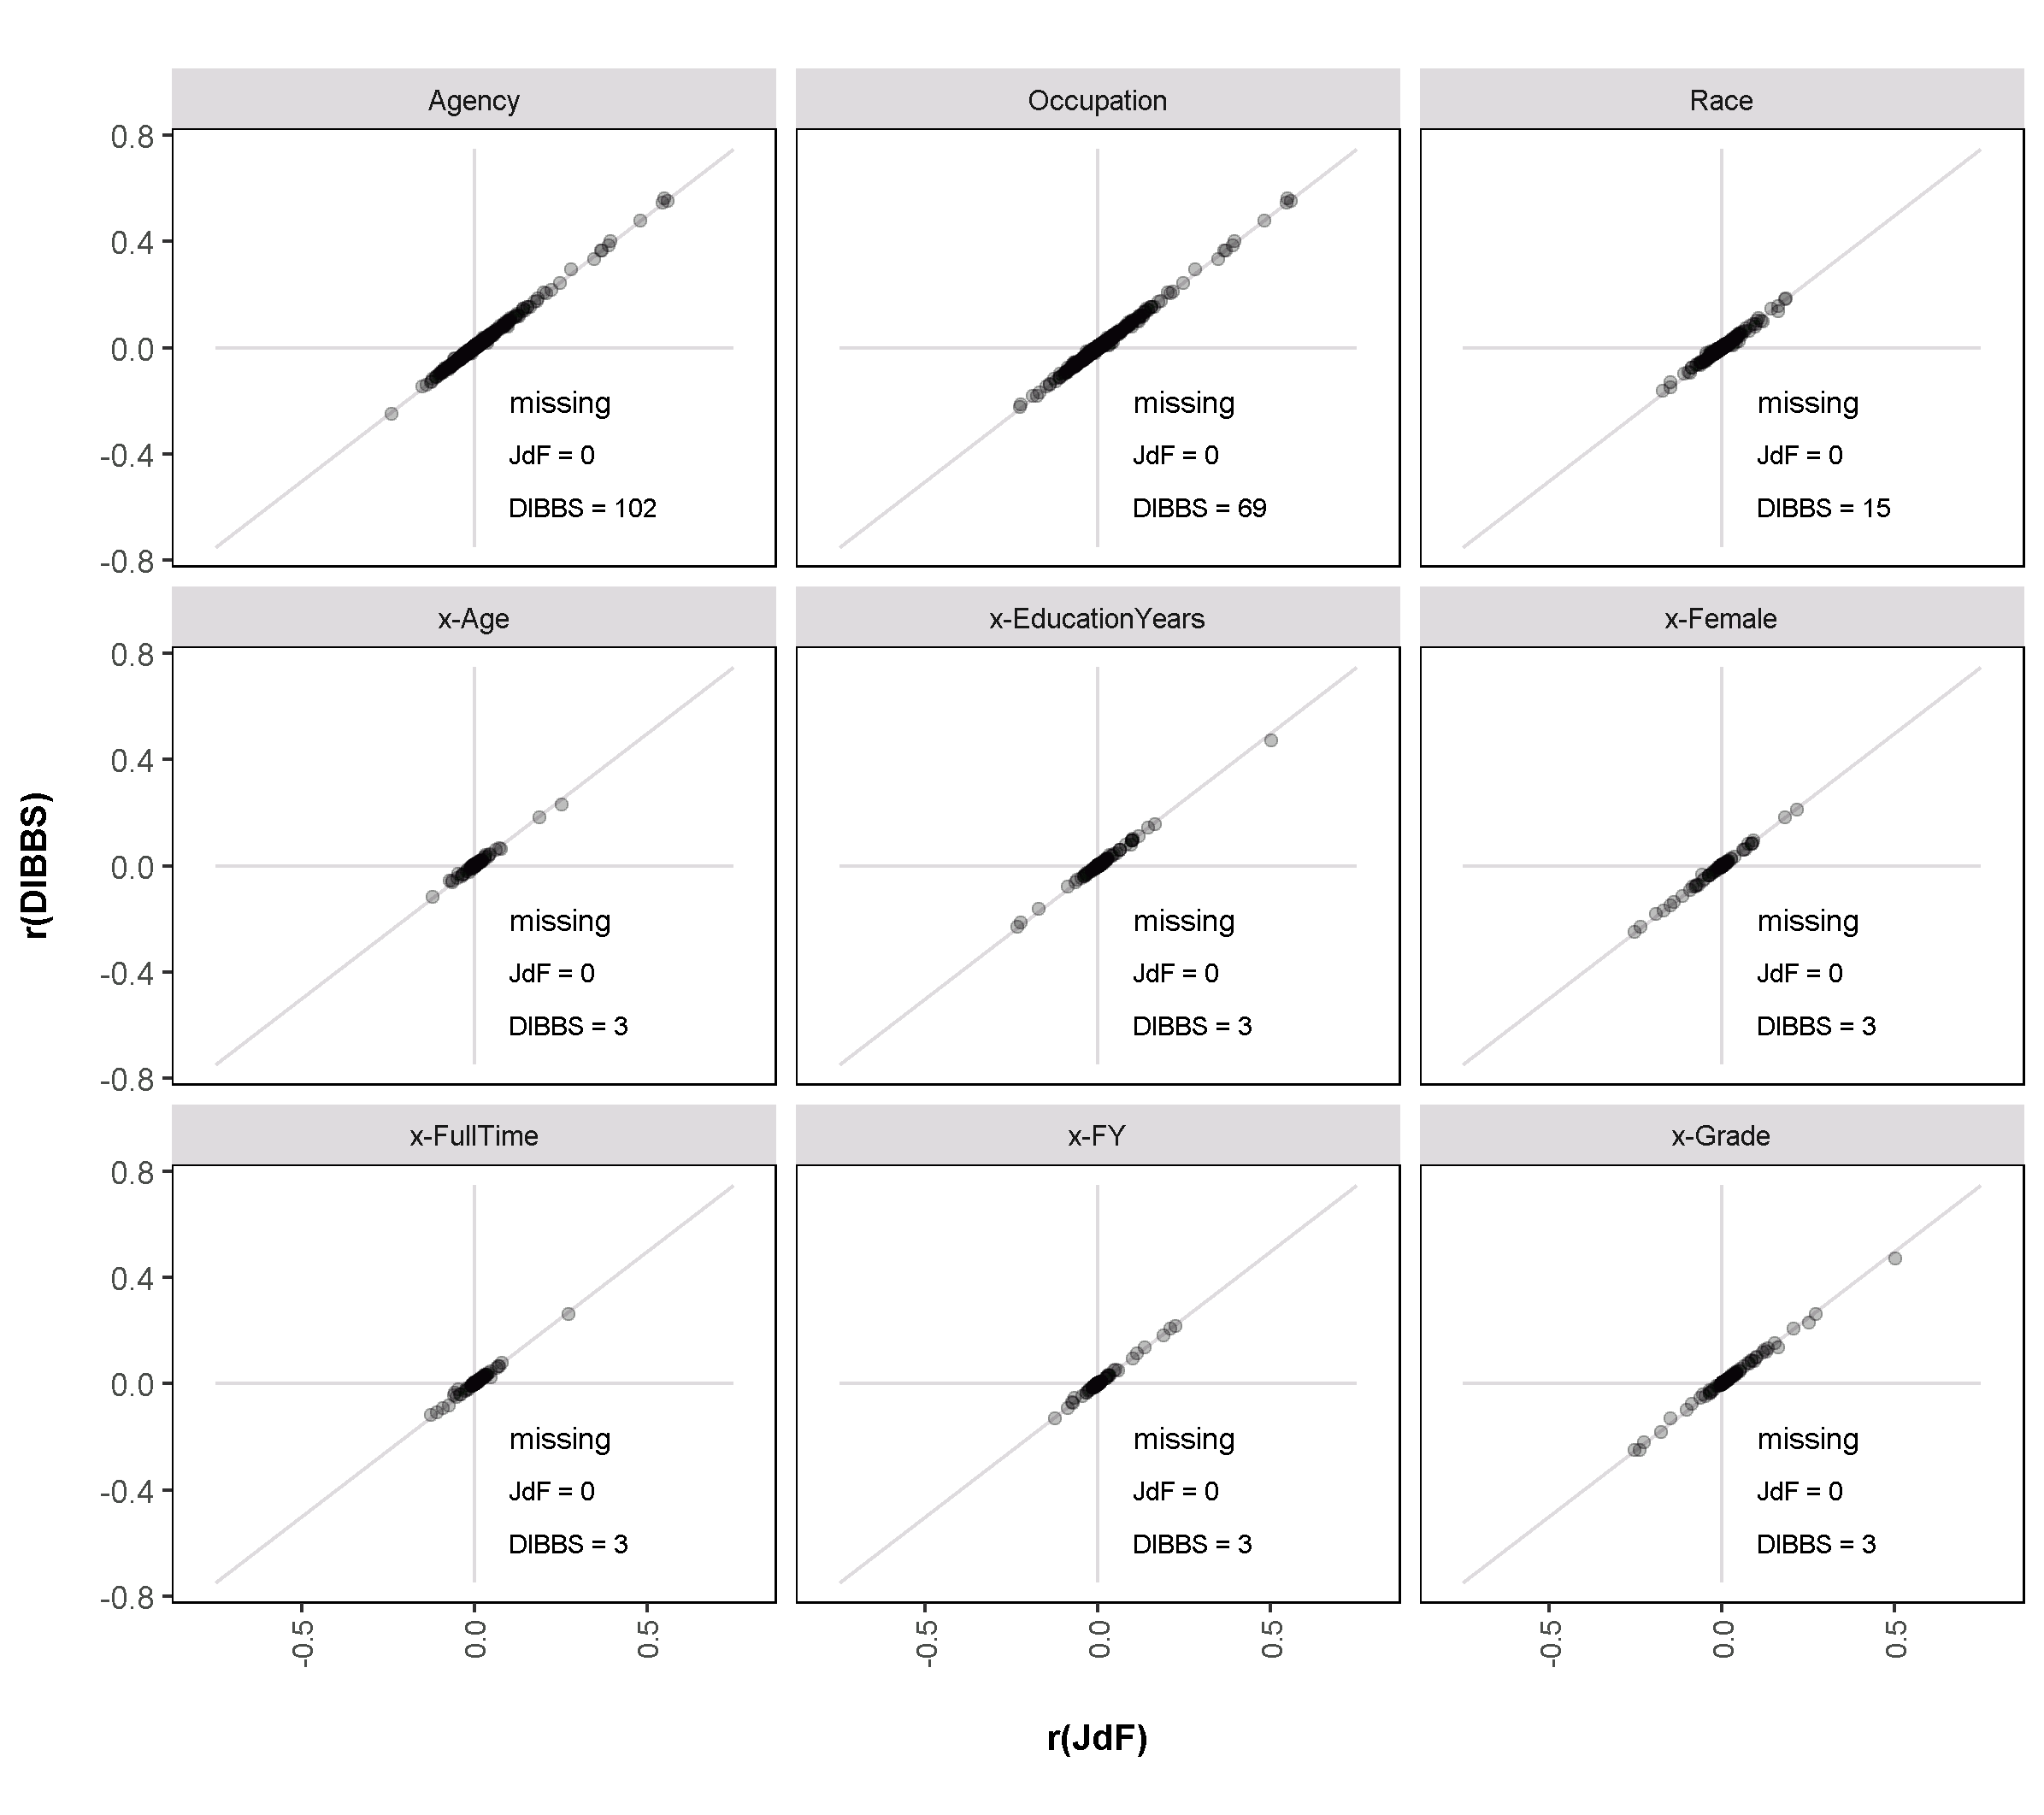
\includegraphics[width=6.5in]{JdFDIBBSCorrelation.png}
    \centering
    \caption{Two variable correlations of corresponding levels of synthetic and authentic data.  Synthetic level correlation on y-axis, corresponding authentic correlation on x-axis.}
    \label{figure:JdFDIBBSCorrelation}
\end{figure}  

\clearpage

CORRELATION OF PRIMARY VARIABLES WITH TWO-VARIABLE INTERACTIONS\\

Figures \ref{figure:JdFDIBBSCorrelationInteraction} and \ref{figure:JdFDIBBSCorrelationInteraction2} show, for pay plan GS, full-time observations, correlations between 1.) the variable indicated in the graph title, 2.) all combinations of levels of the variable listed in a title bar, and 3.) all levels of other variables appearing in the title bars.  These constitute correlation of main variables with two variable interactions.  In the case of categorical variables, or fixed effects, this is the association of a primary variable with the proportion of observations in interacting level combinations of two other variables.  Agency and occupation truncated to first two positions.\\

Observation:  Proximity of all points to slope 1.0 reference line indicates agreement of three-variable associations between data sets and implies depth of utility beyond simple pairwise relationships.\\

\begin{figure}[ht]
    \centering
    \begin{subfigure}{.5\textwidth}
        \centering
        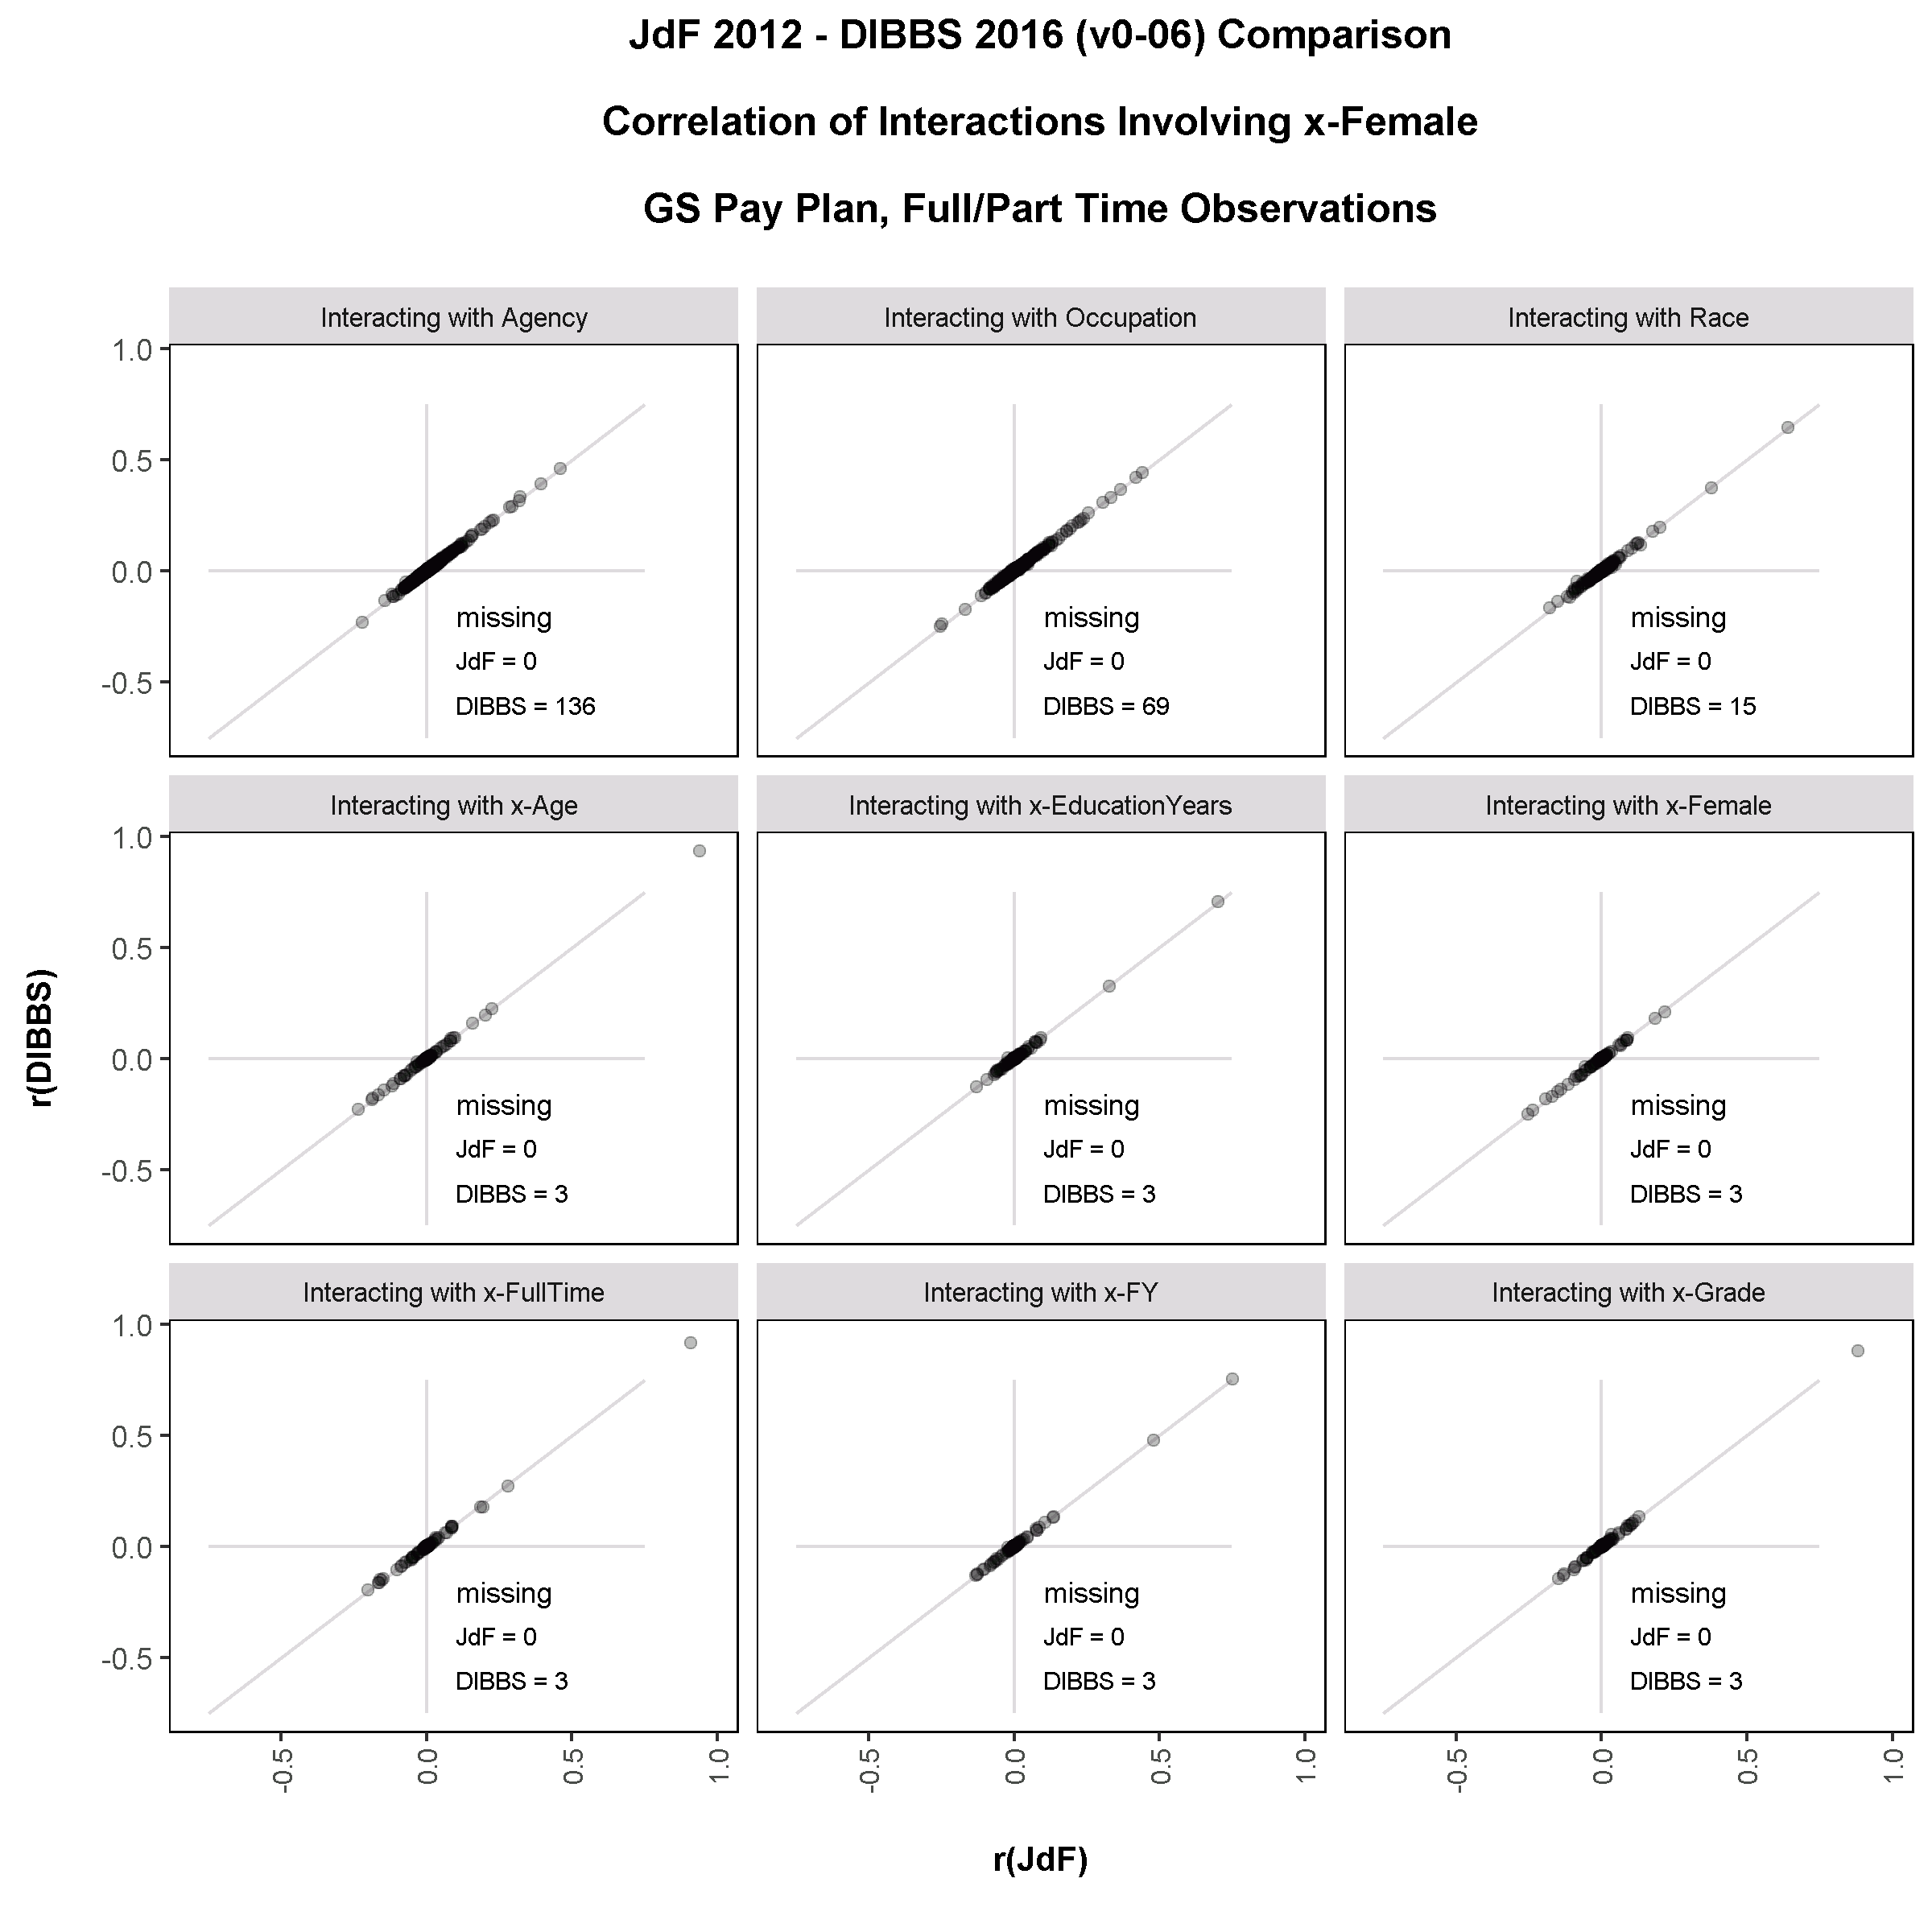
\includegraphics[width=3in, trim={0 0.25in 0 1in}, clip]{JdFDIBBSCorrelationInteraction-x-Female.png}
        \caption{Correlations involving sex}
        %\label{figure:}
        \vspace{10pt}
    \end{subfigure}% suppress line break
    \begin{subfigure}{.5\textwidth}
        \centering
        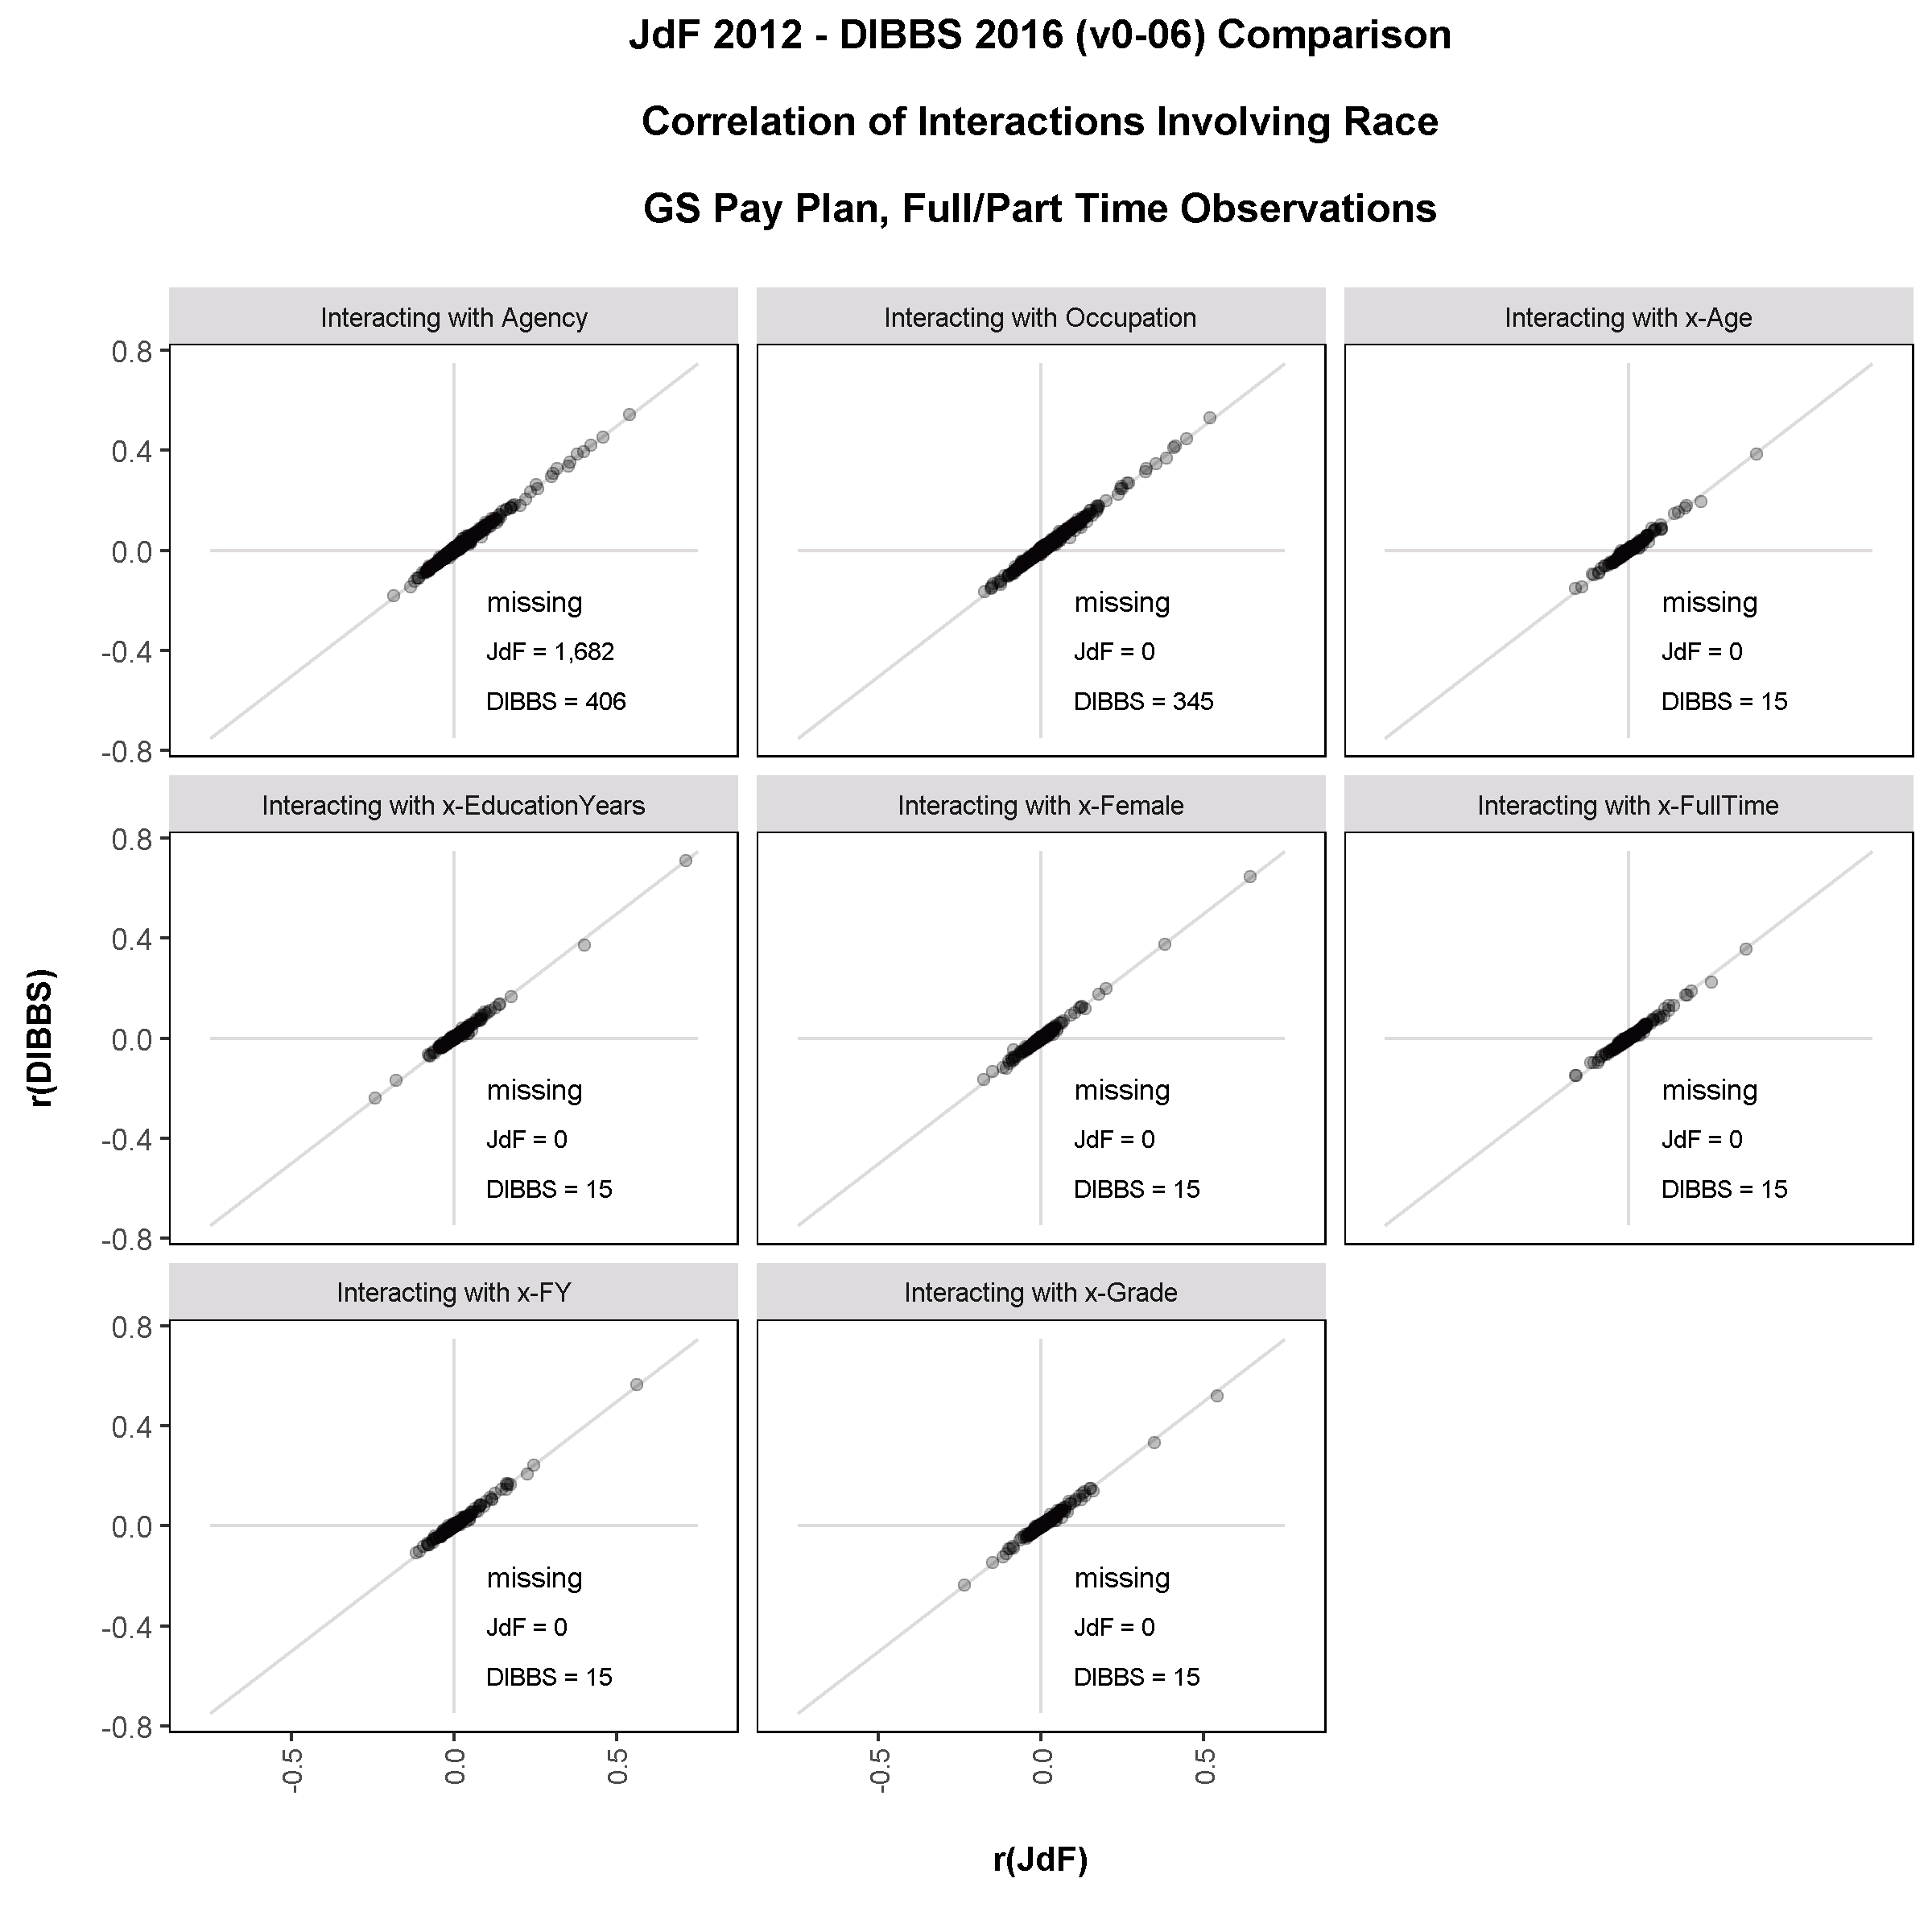
\includegraphics[width=3in, trim={0 0.25in 0 1in}, clip]{JdFDIBBSCorrelationInteraction-Race.png}
        \caption{Correlations involving race}
        %\label{figure:}
        \vspace{10pt}
    \end{subfigure}
    \begin{subfigure}{.5\textwidth}
        \centering
        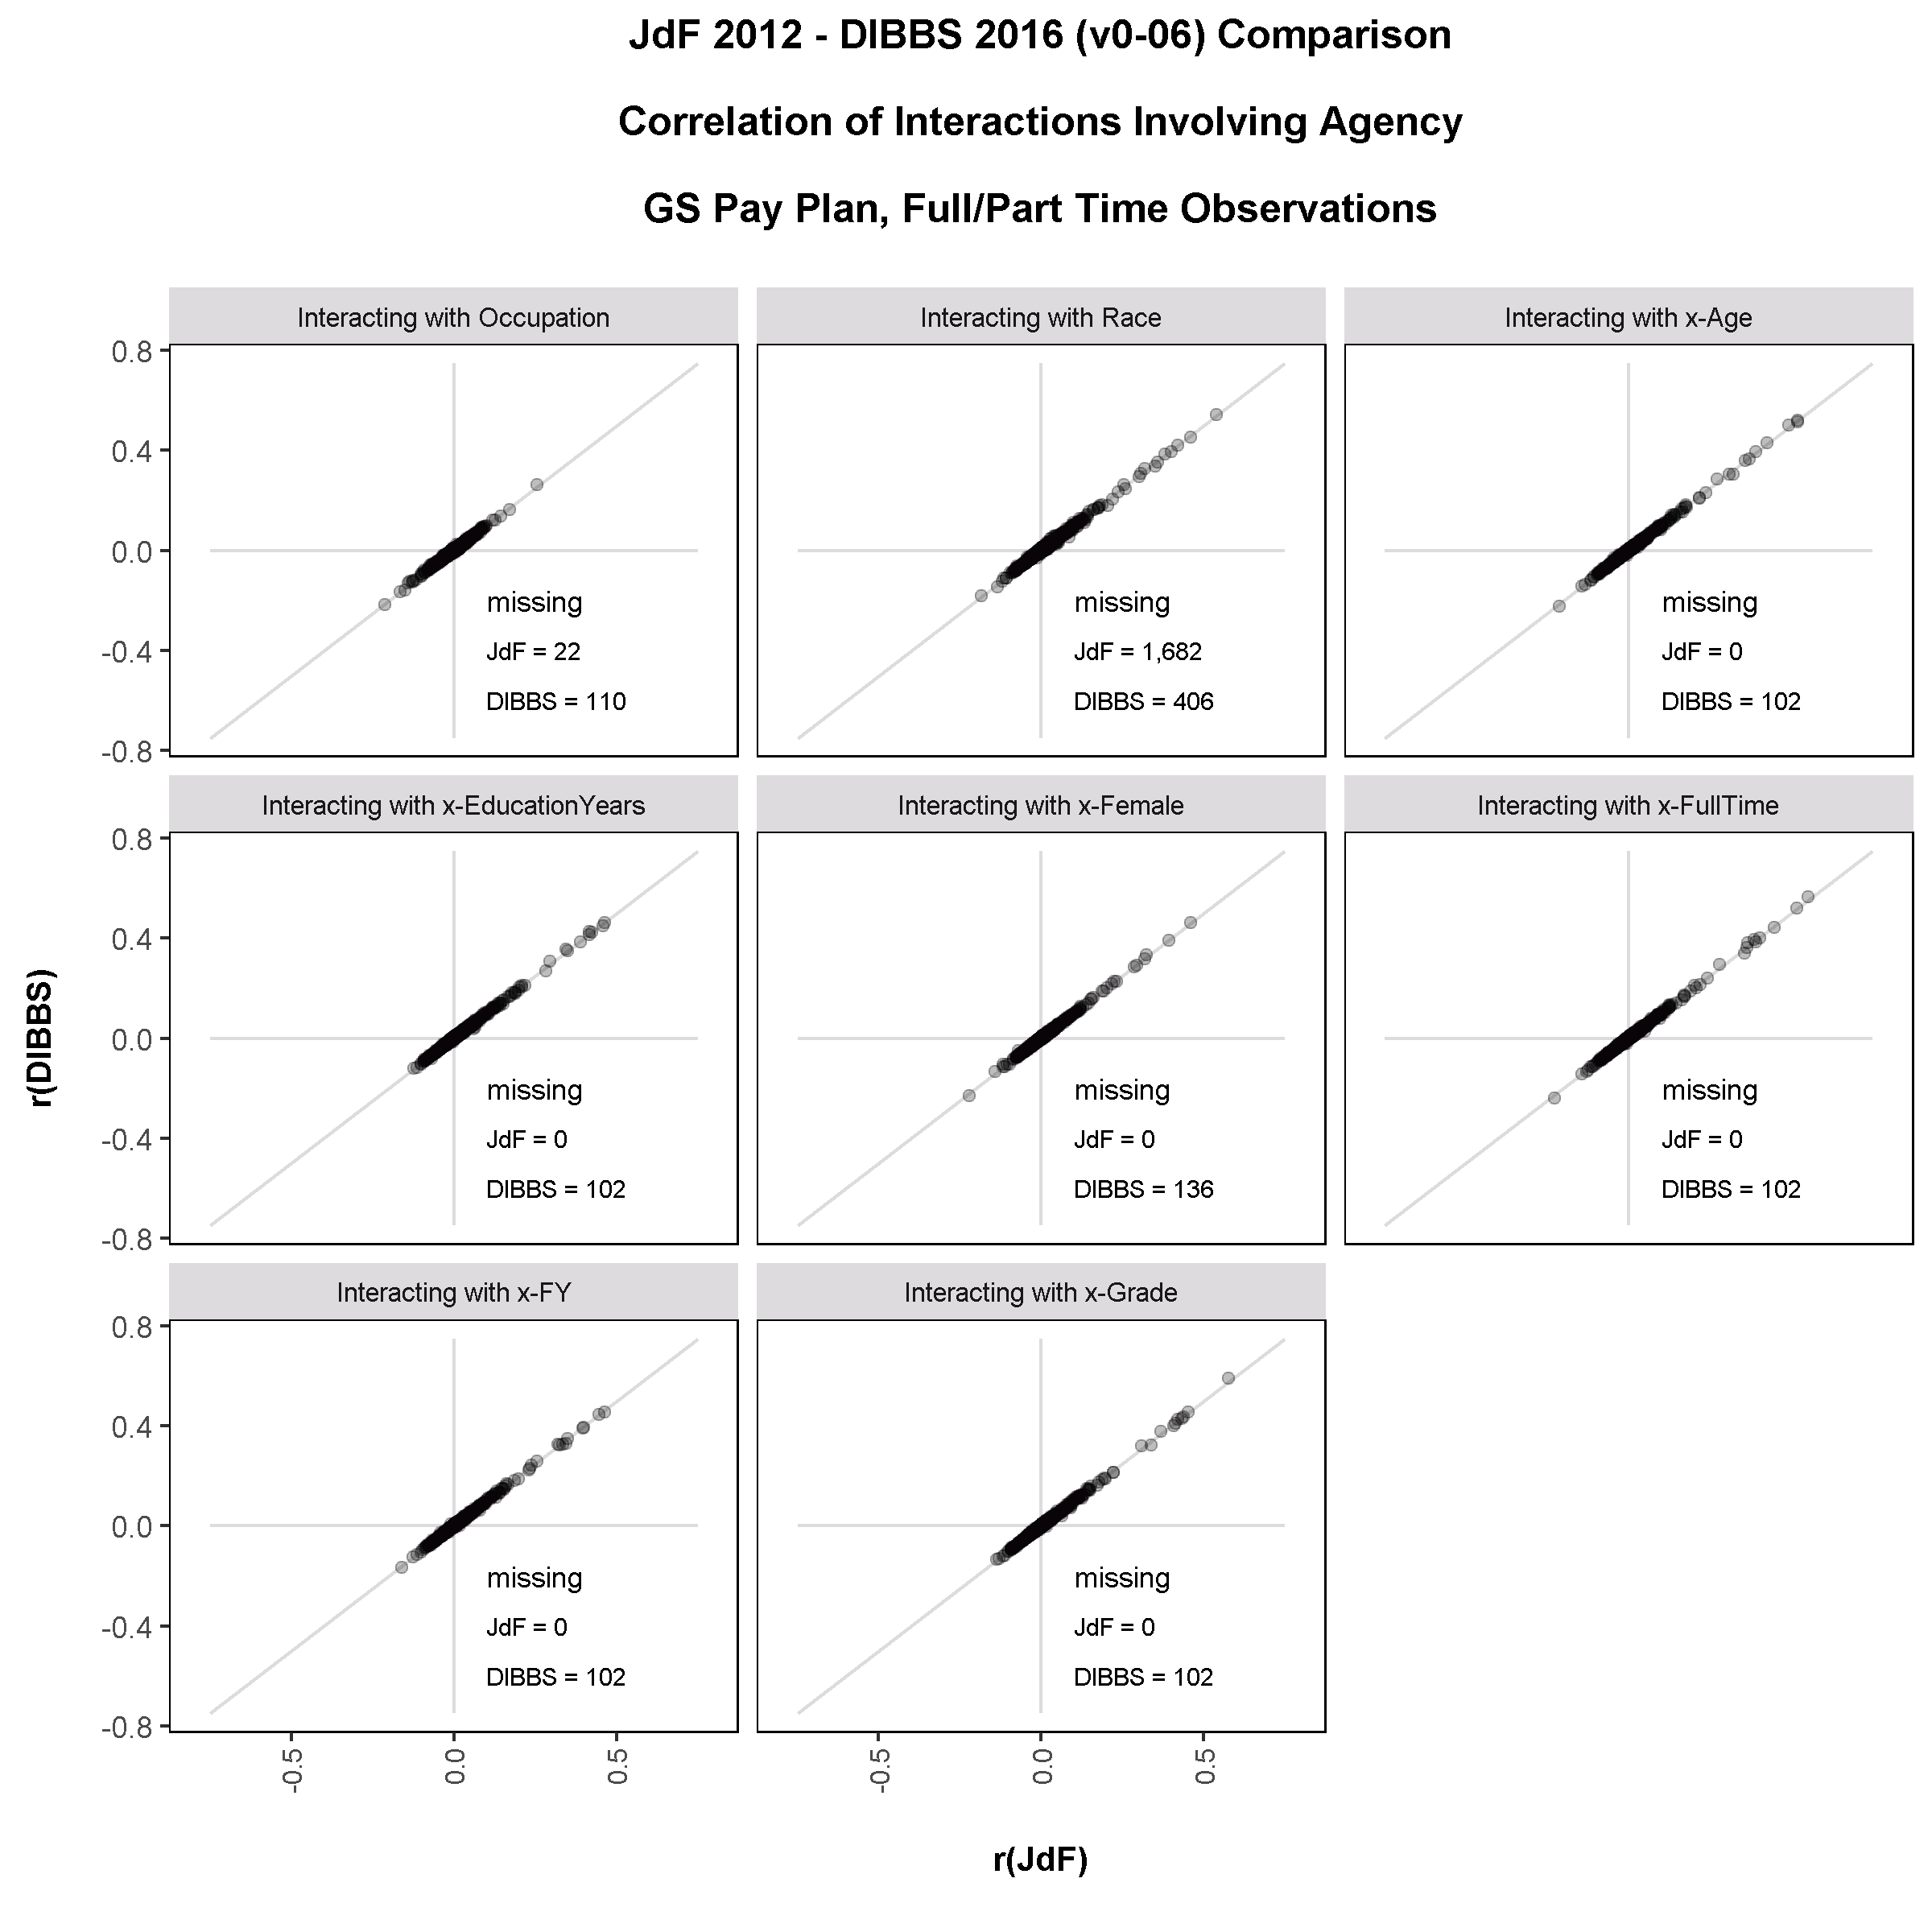
\includegraphics[width=3in, trim={0 0.25in 0 1in}, clip]{JdFDIBBSCorrelationInteraction-Agency.png}
        \caption{Correlations involving agency}
        %\label{figure:}
        \vspace{10pt}
    \end{subfigure}% suppress line break
    \begin{subfigure}{.5\textwidth}
        \centering
        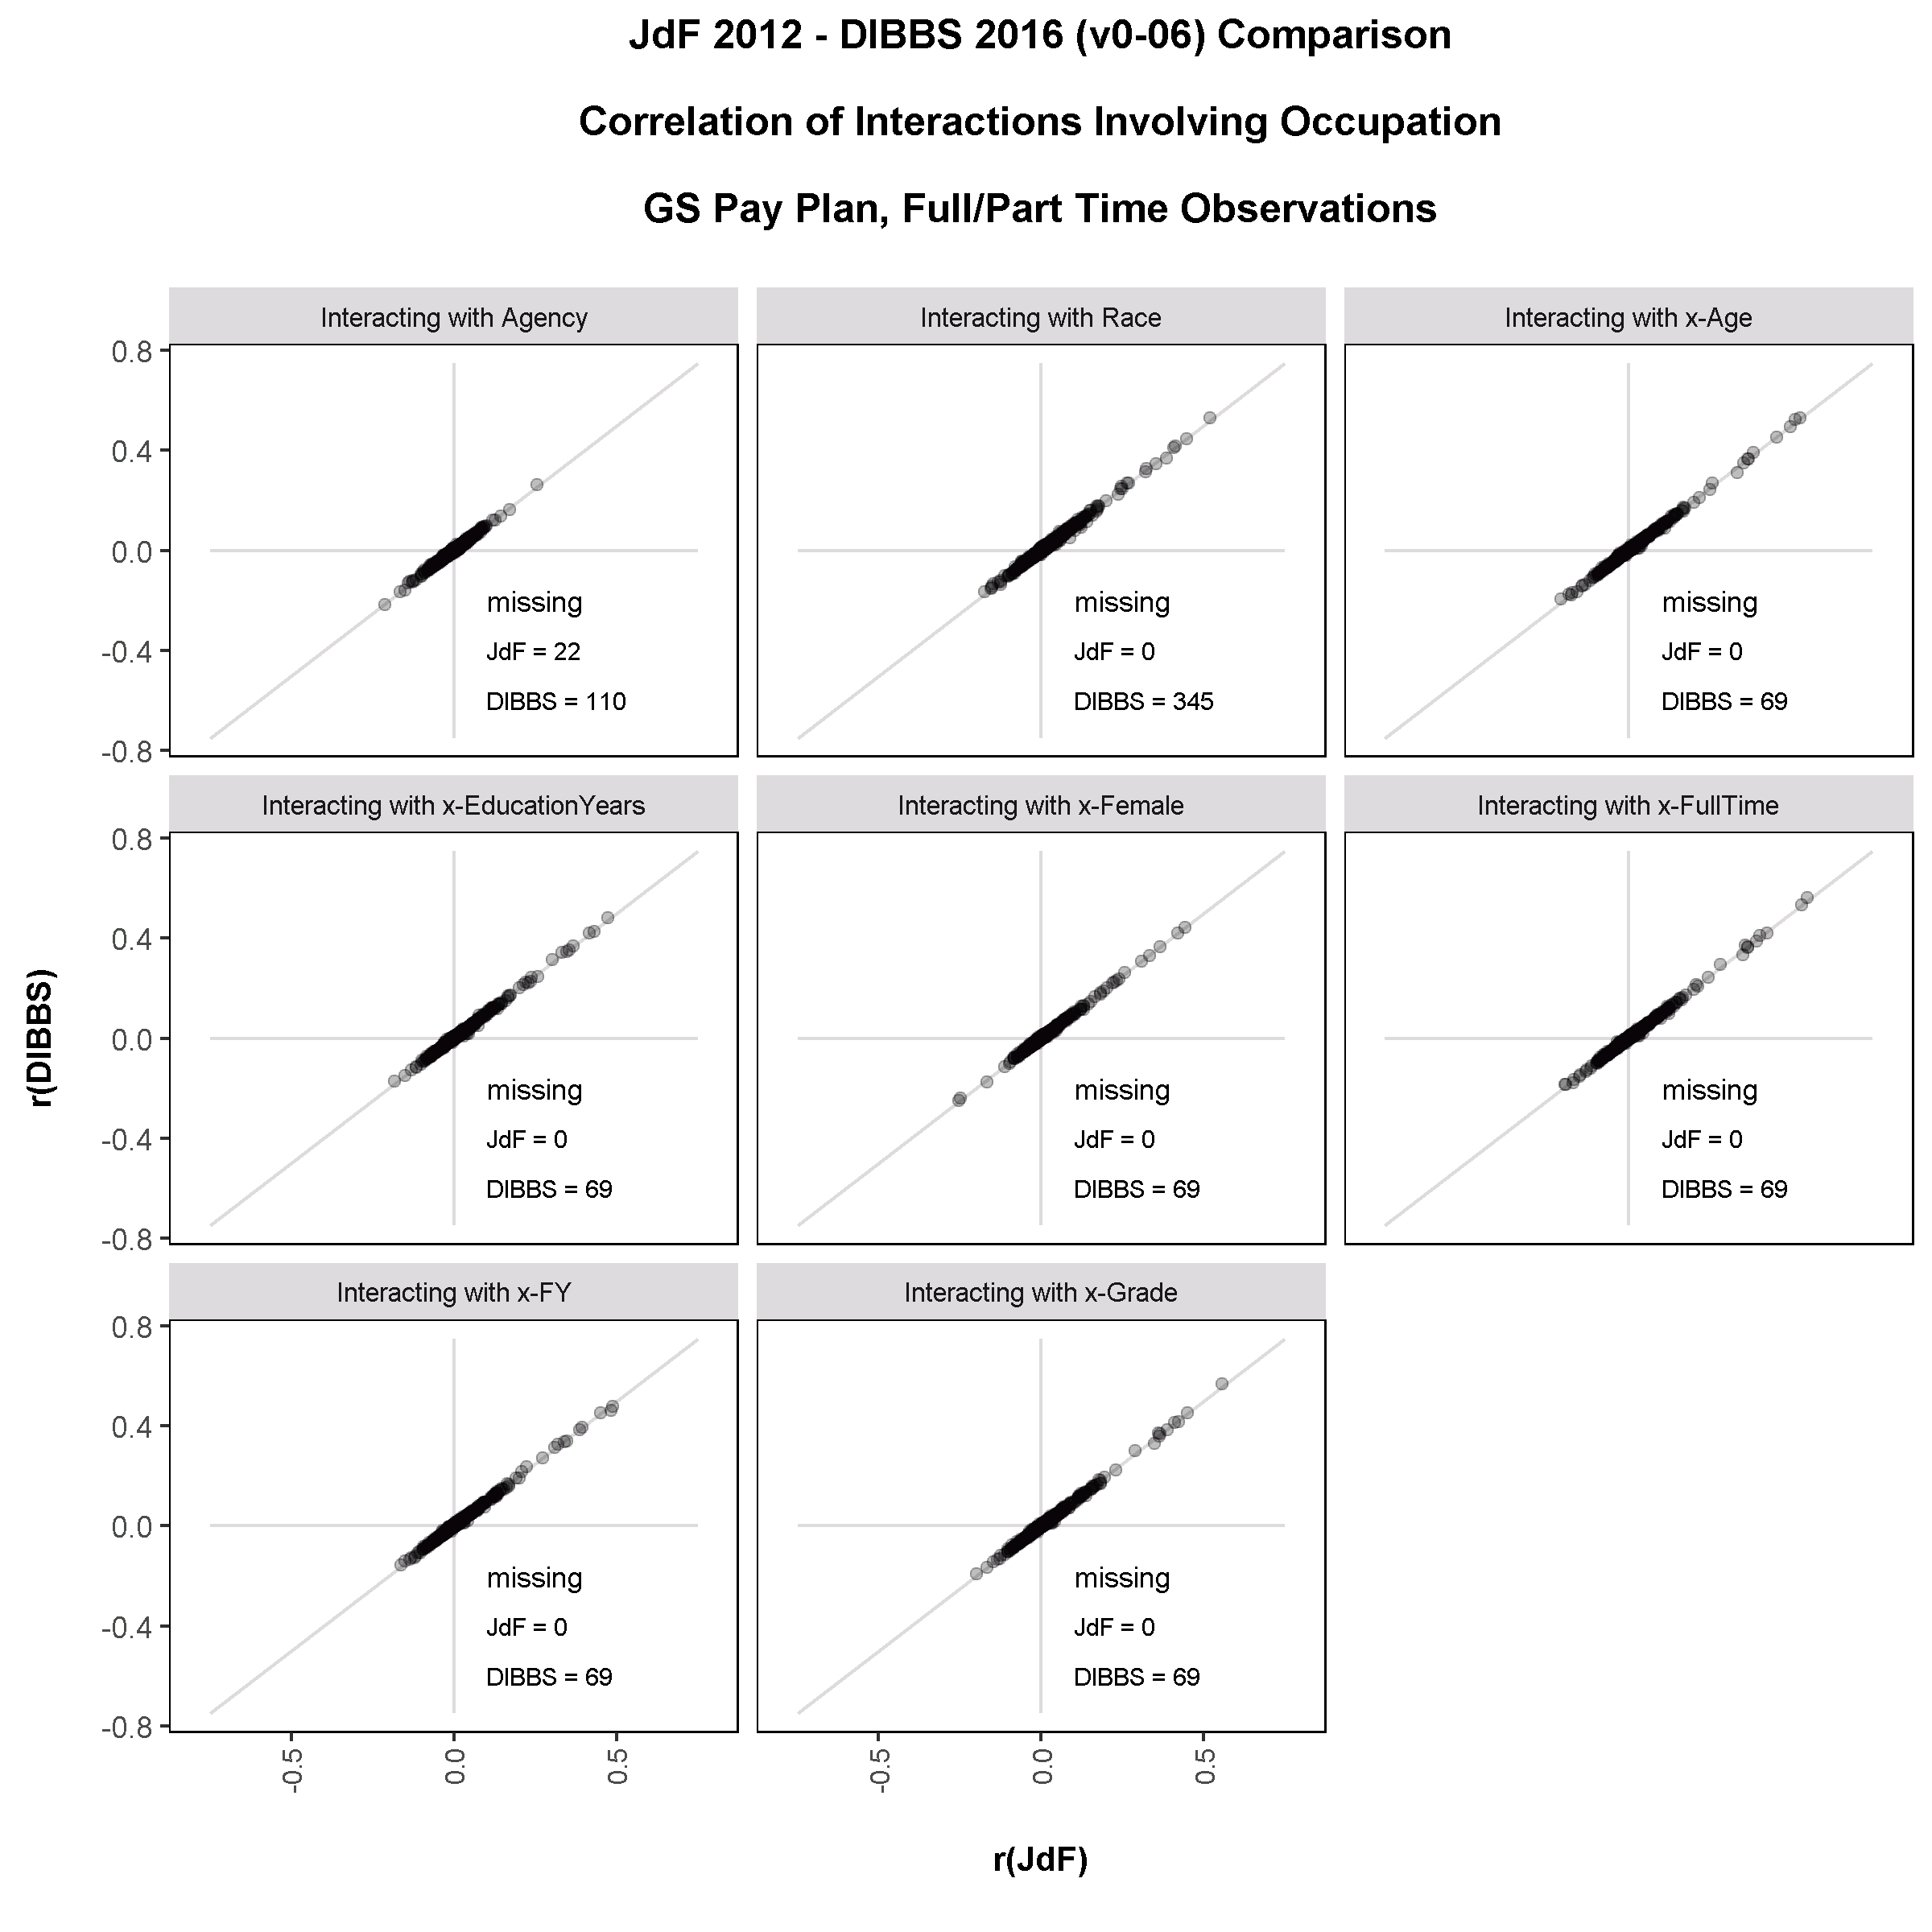
\includegraphics[width=3in, trim={0 0.25in 0 1in}, clip]{JdFDIBBSCorrelationInteraction-Occupation.png}
        \caption{Correlations involving occupation}
        %\label{figure:}
        \vspace{10pt}
    \end{subfigure}
    \caption{Correlations of primary variables with two variable interactions.  Variable set one.  Synthetic level correlation on y-axis, corresponding authentic correlation on x-axis.}
    \label{figure:JdFDIBBSCorrelationInteraction}
\end{figure}

\begin{figure}[ht]
    \centering
    \begin{subfigure}{.5\textwidth}
        \centering
        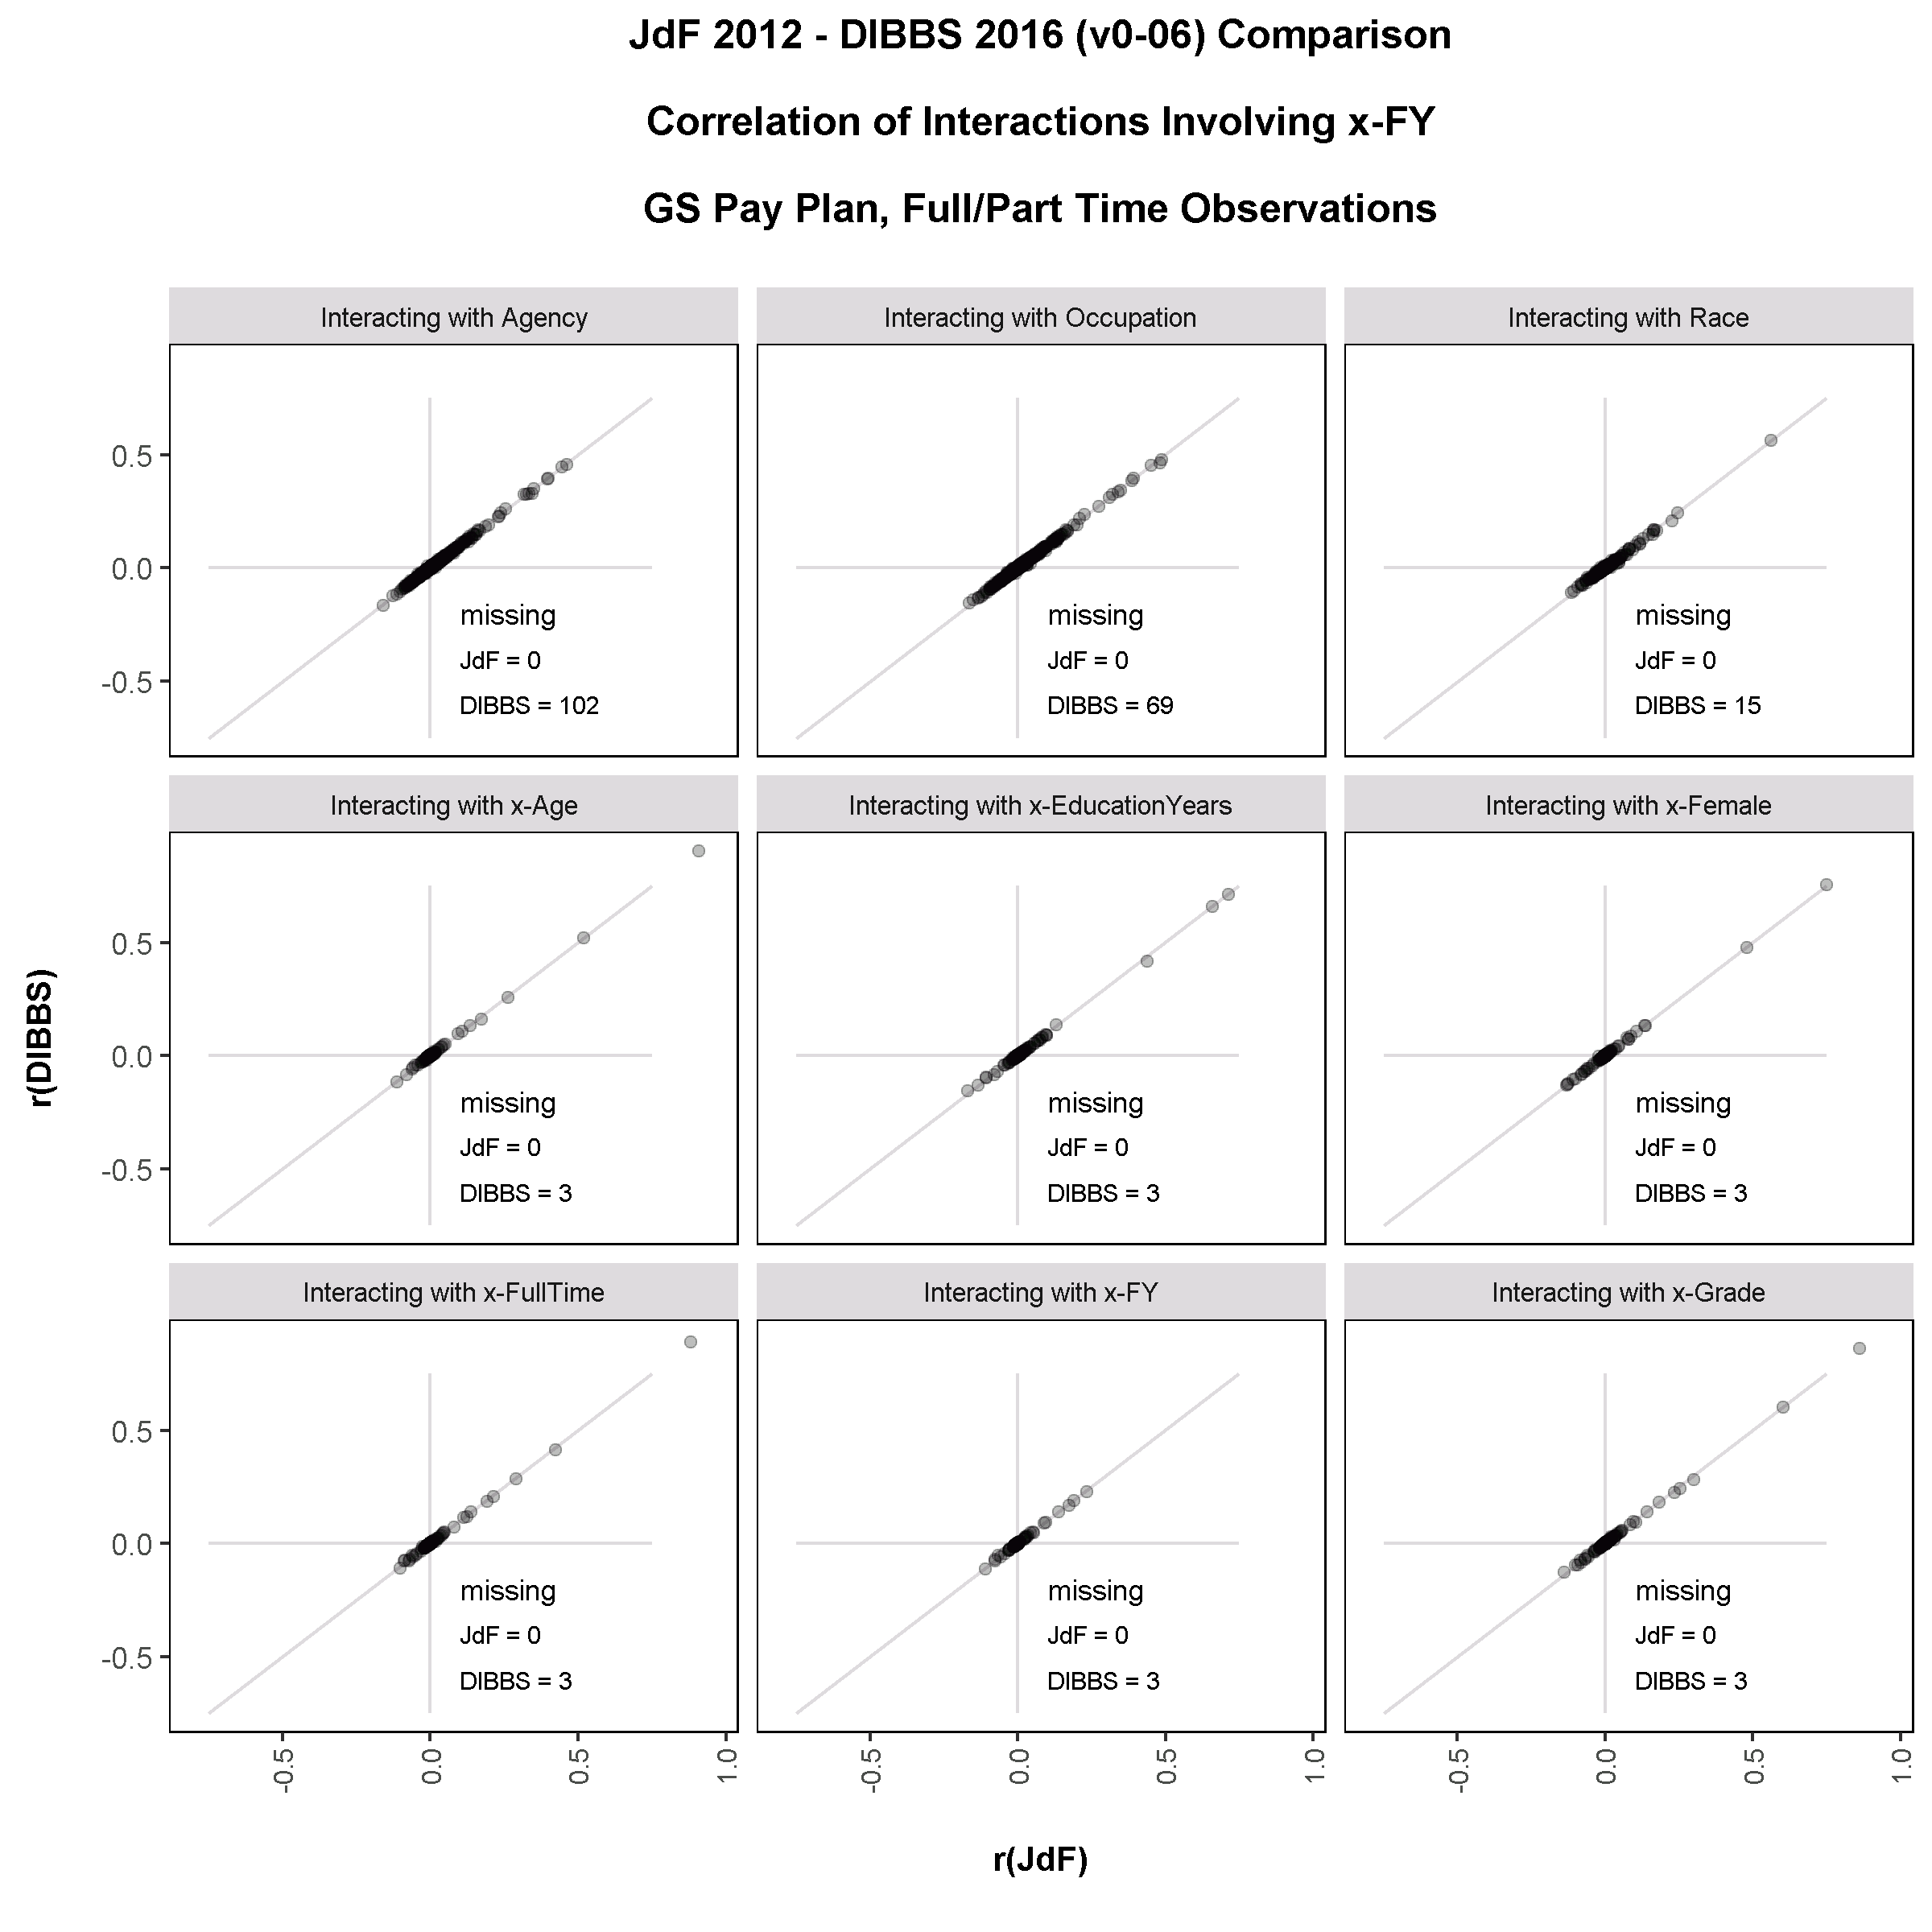
\includegraphics[width=3in, trim={0 0.25in 0 1in}, clip]{JdFDIBBSCorrelationInteraction-x-FY.png}
        \caption{Correlations involving Fiscal Year}
        %\label{figure:}
        \vspace{10pt}
    \end{subfigure}% suppress line break
    \begin{subfigure}{.5\textwidth}
        \centering
        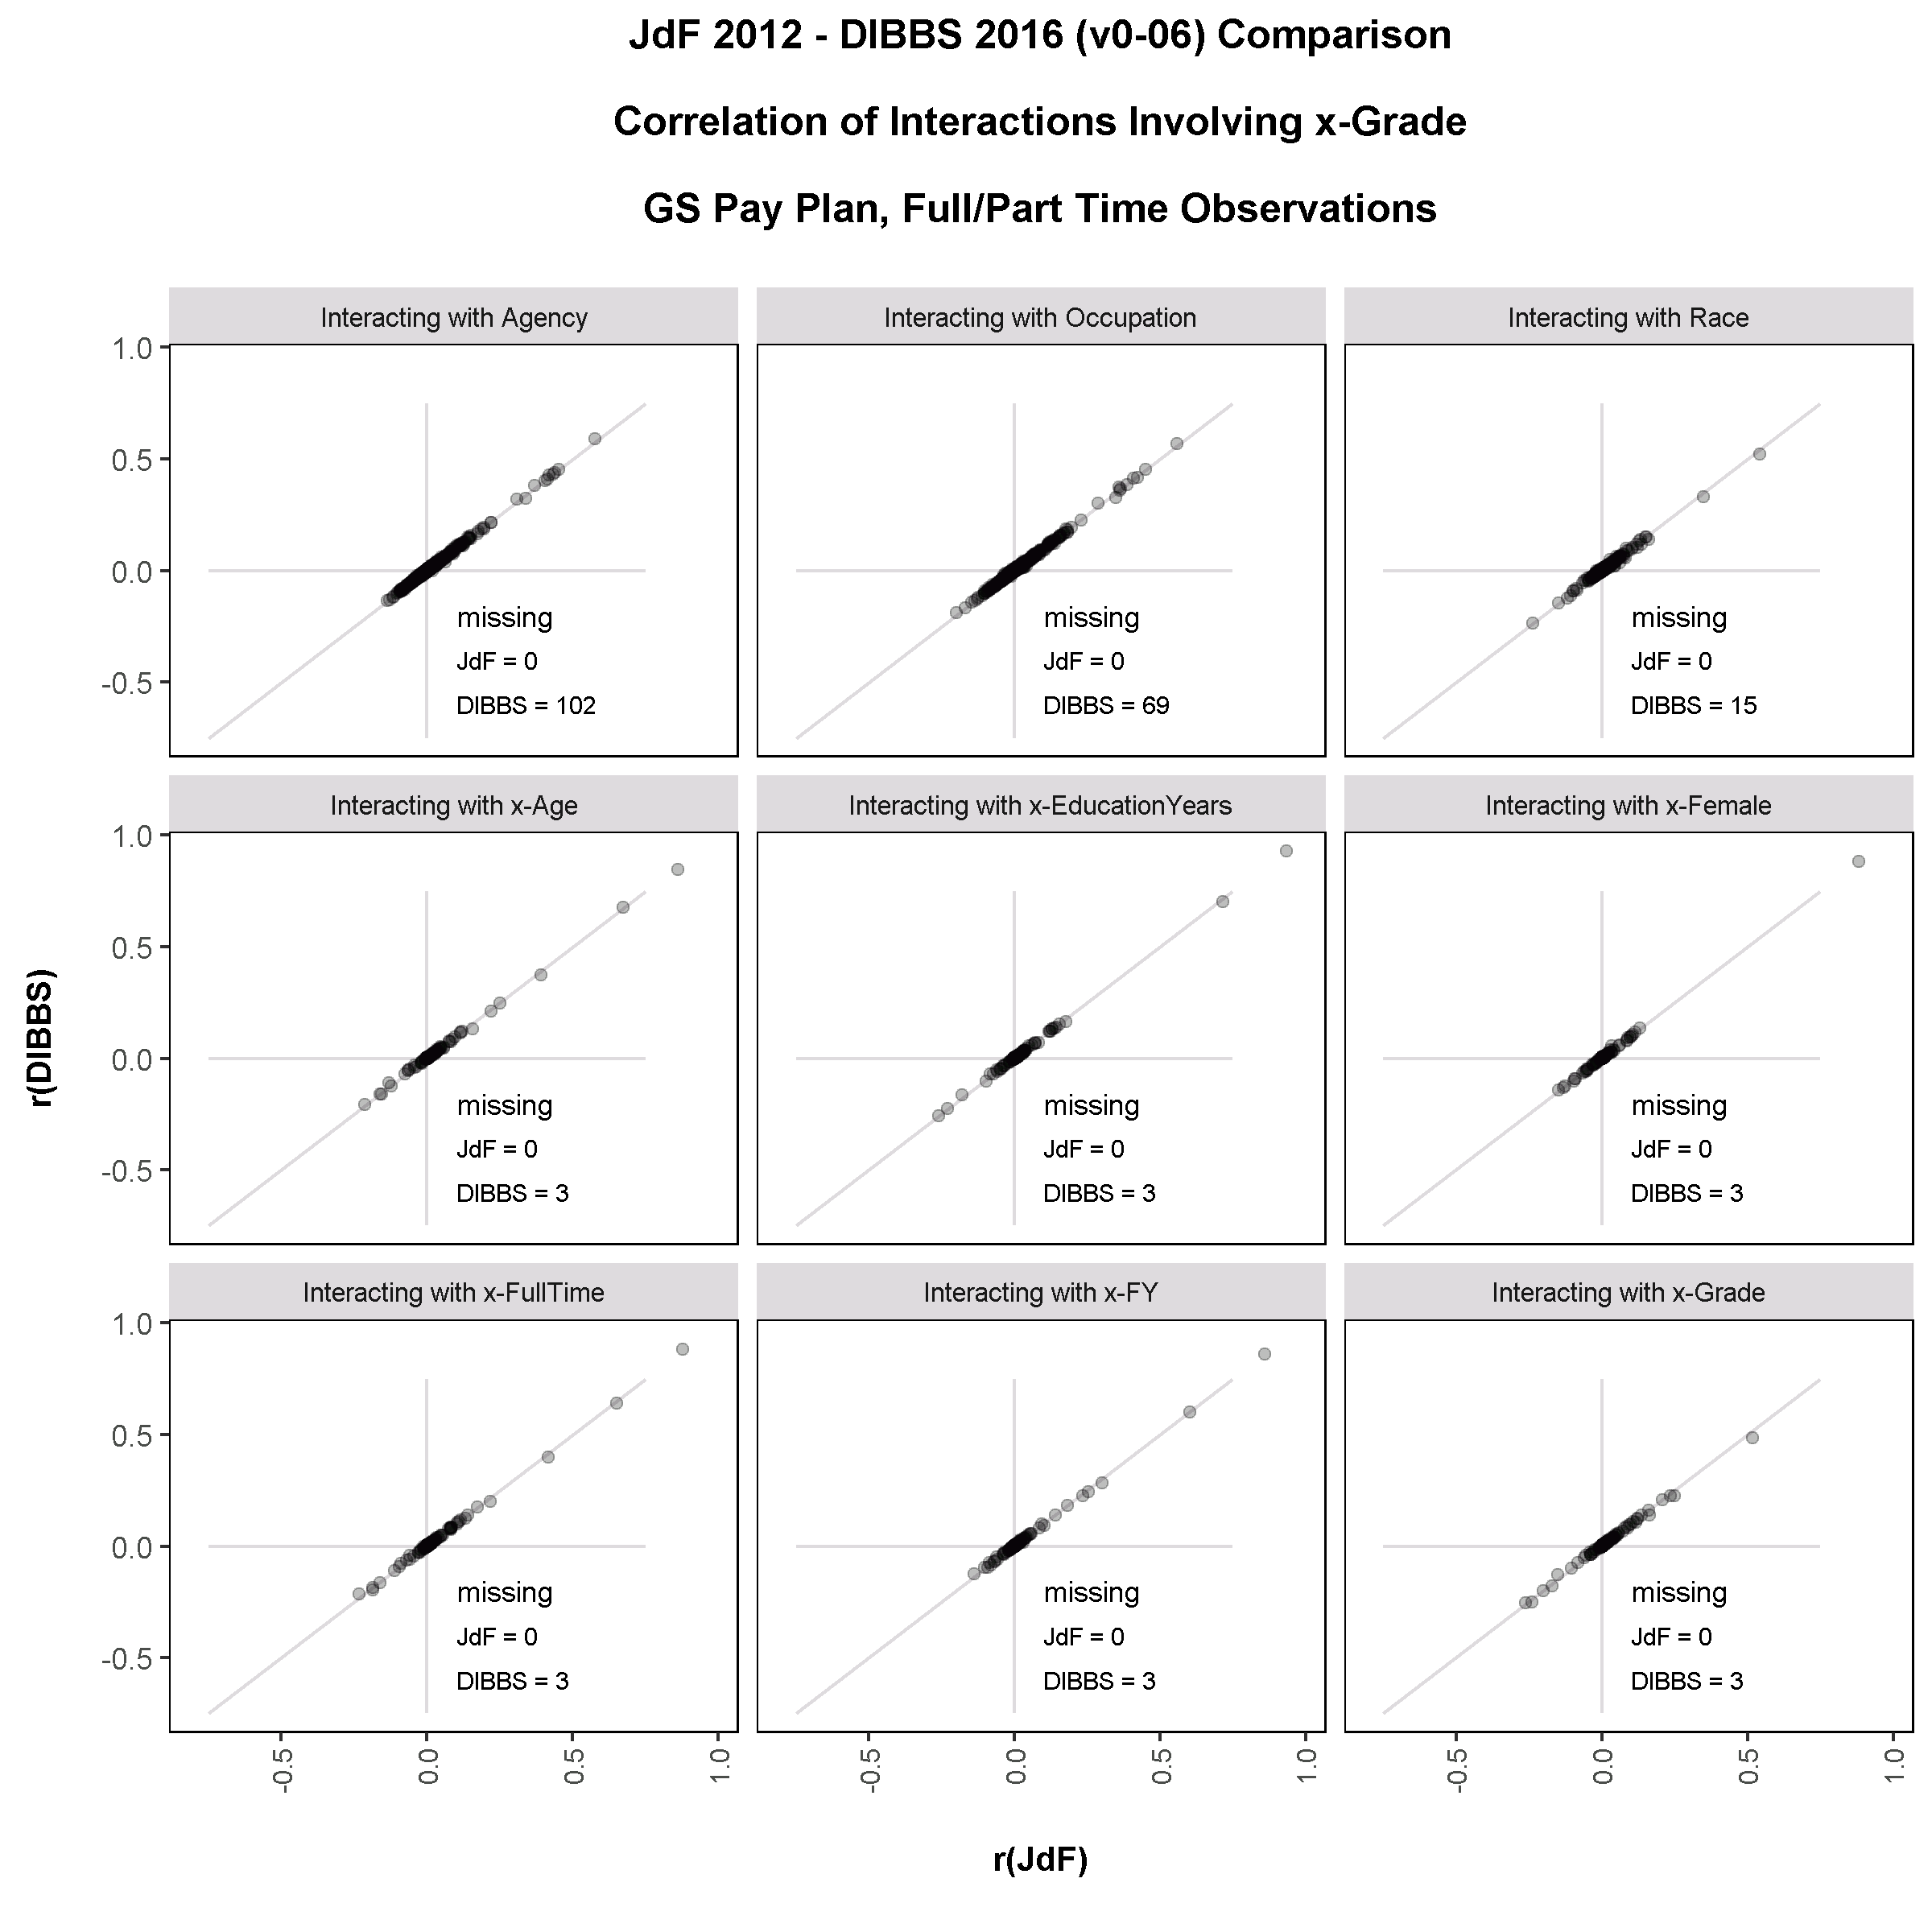
\includegraphics[width=3in, trim={0 0.25in 0 1in}, clip]{JdFDIBBSCorrelationInteraction-x-Grade.png}
        \caption{Correlations involving Grade}
        %\label{figure:}
        \vspace{10pt}
    \end{subfigure}
    \begin{subfigure}{.5\textwidth}
        \centering
        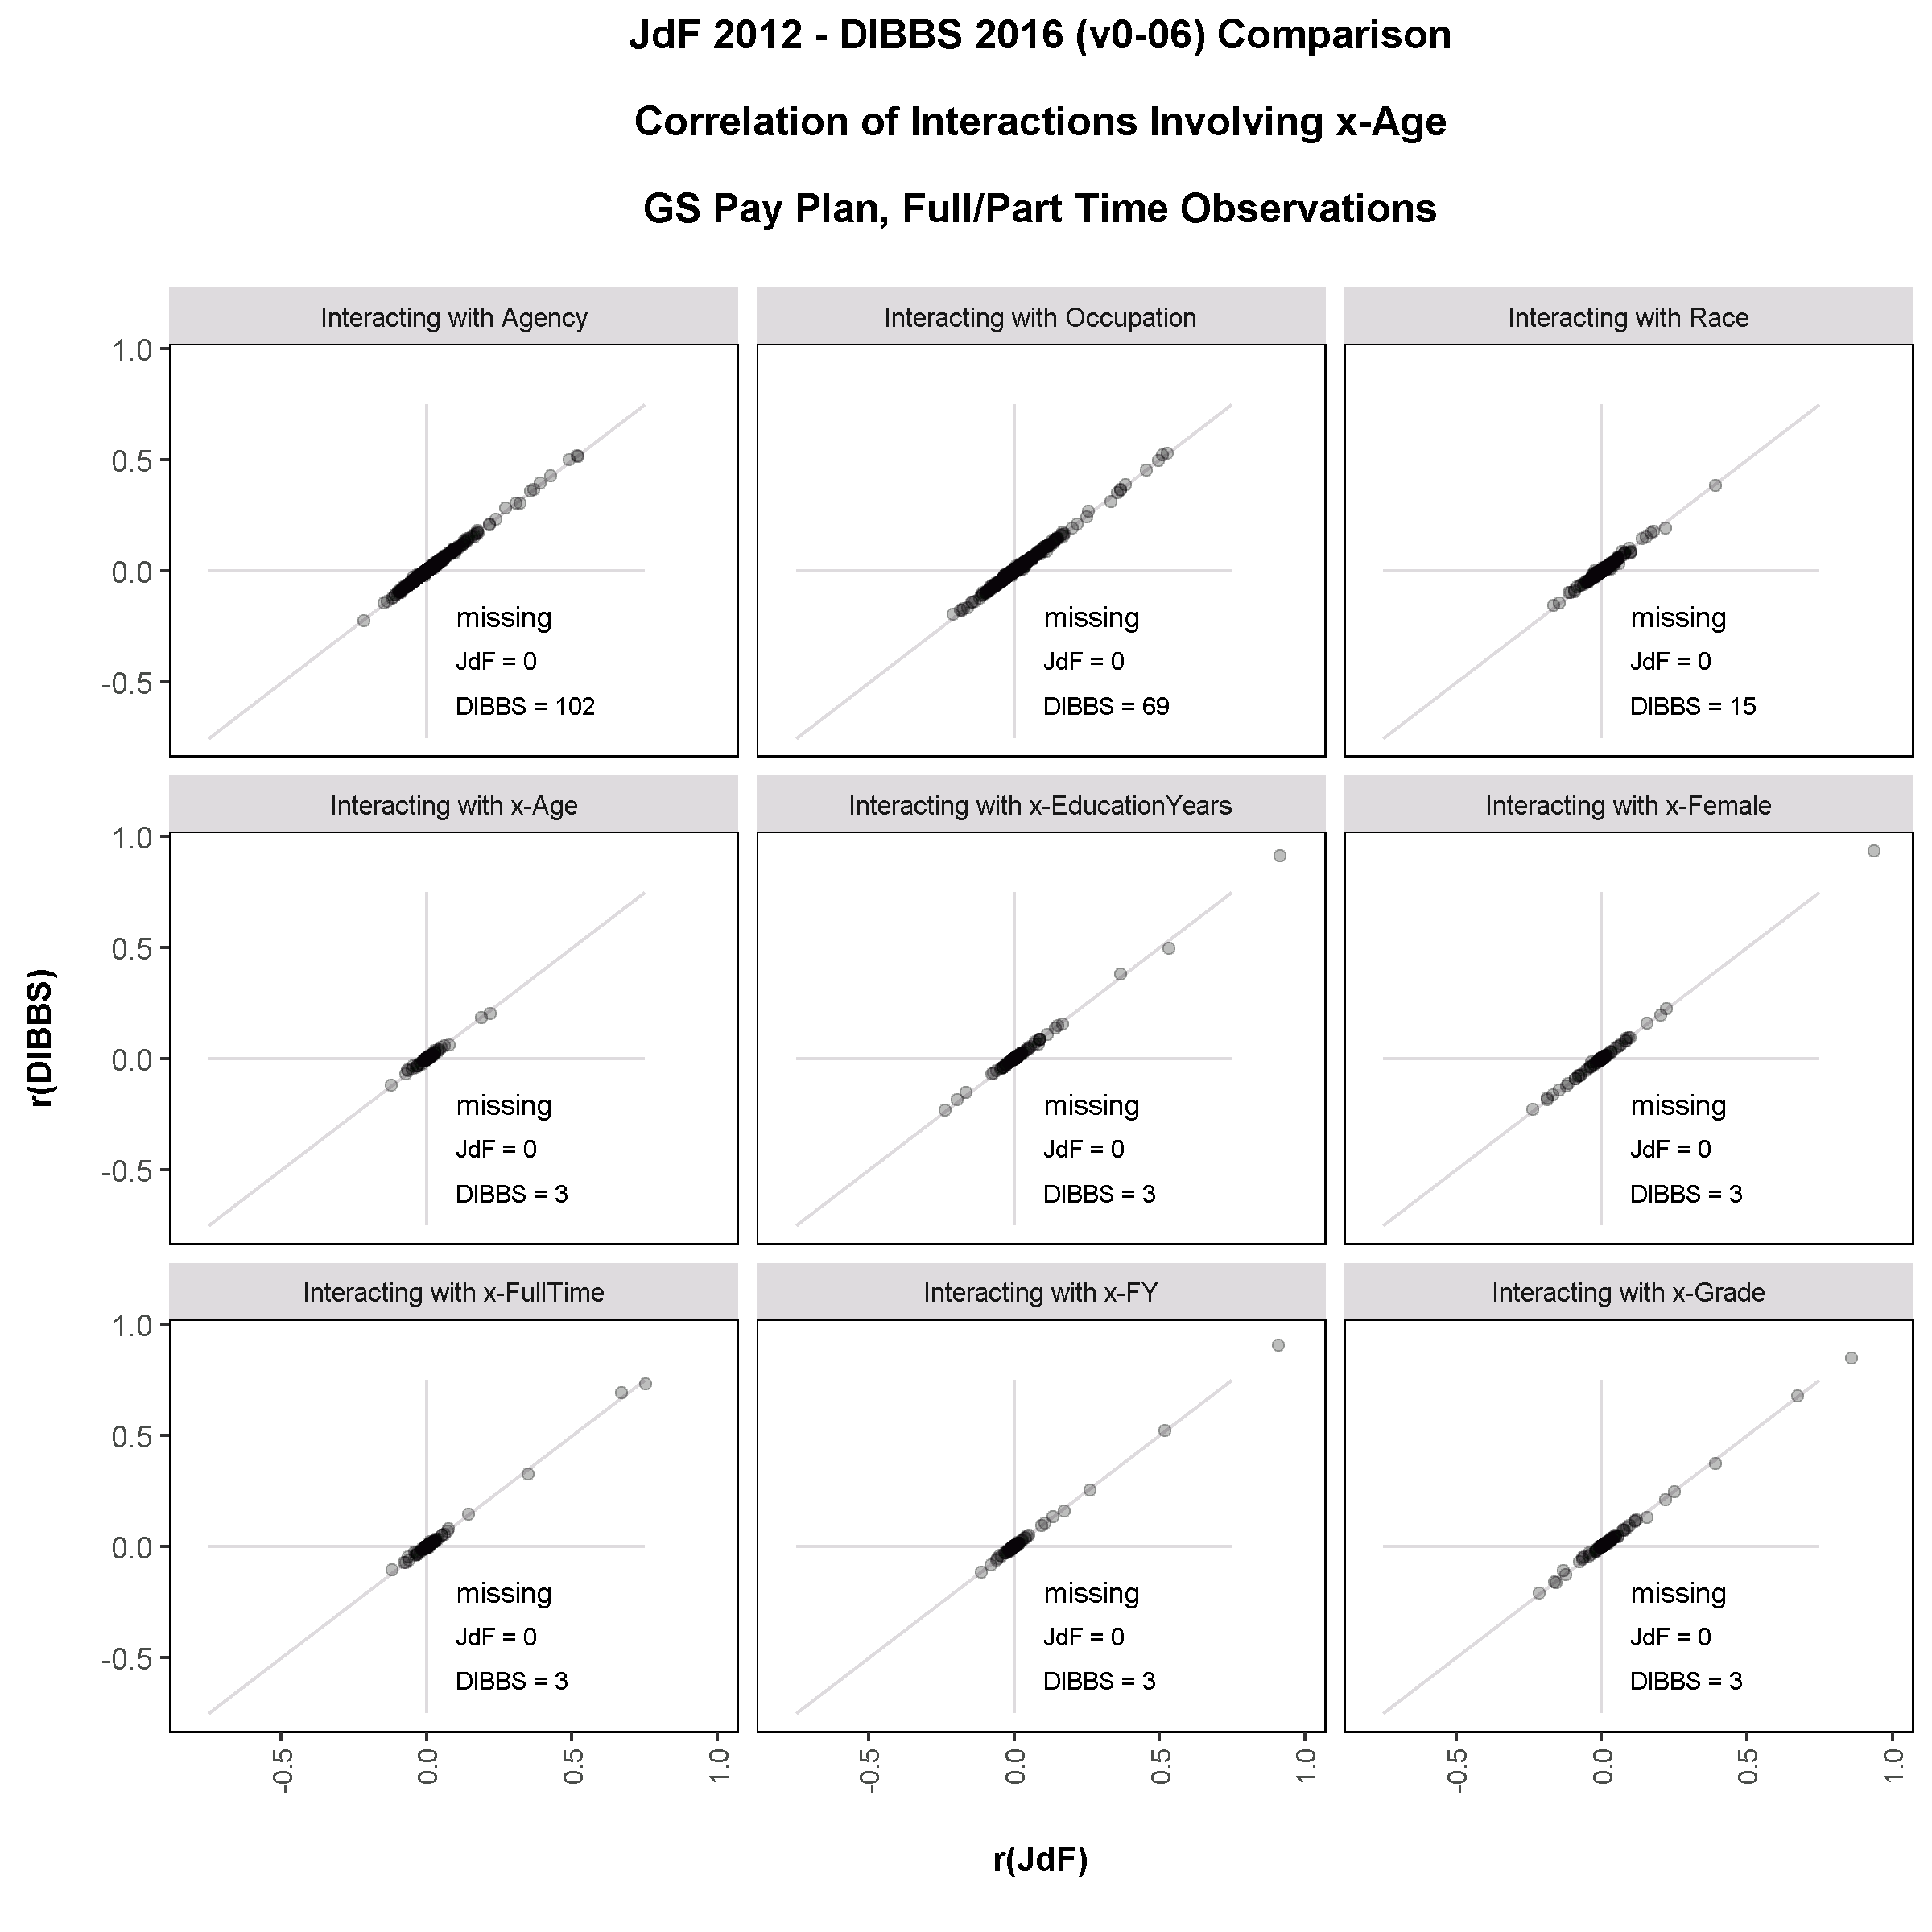
\includegraphics[width=3in, trim={0 0.25in 0 1in}, clip]{JdFDIBBSCorrelationInteraction-x-Age.png}
        \caption{Correlations involving Age}
        %\label{figure:}
        \vspace{10pt}
    \end{subfigure}% suppress line break
    \begin{subfigure}{.5\textwidth}
        \centering
        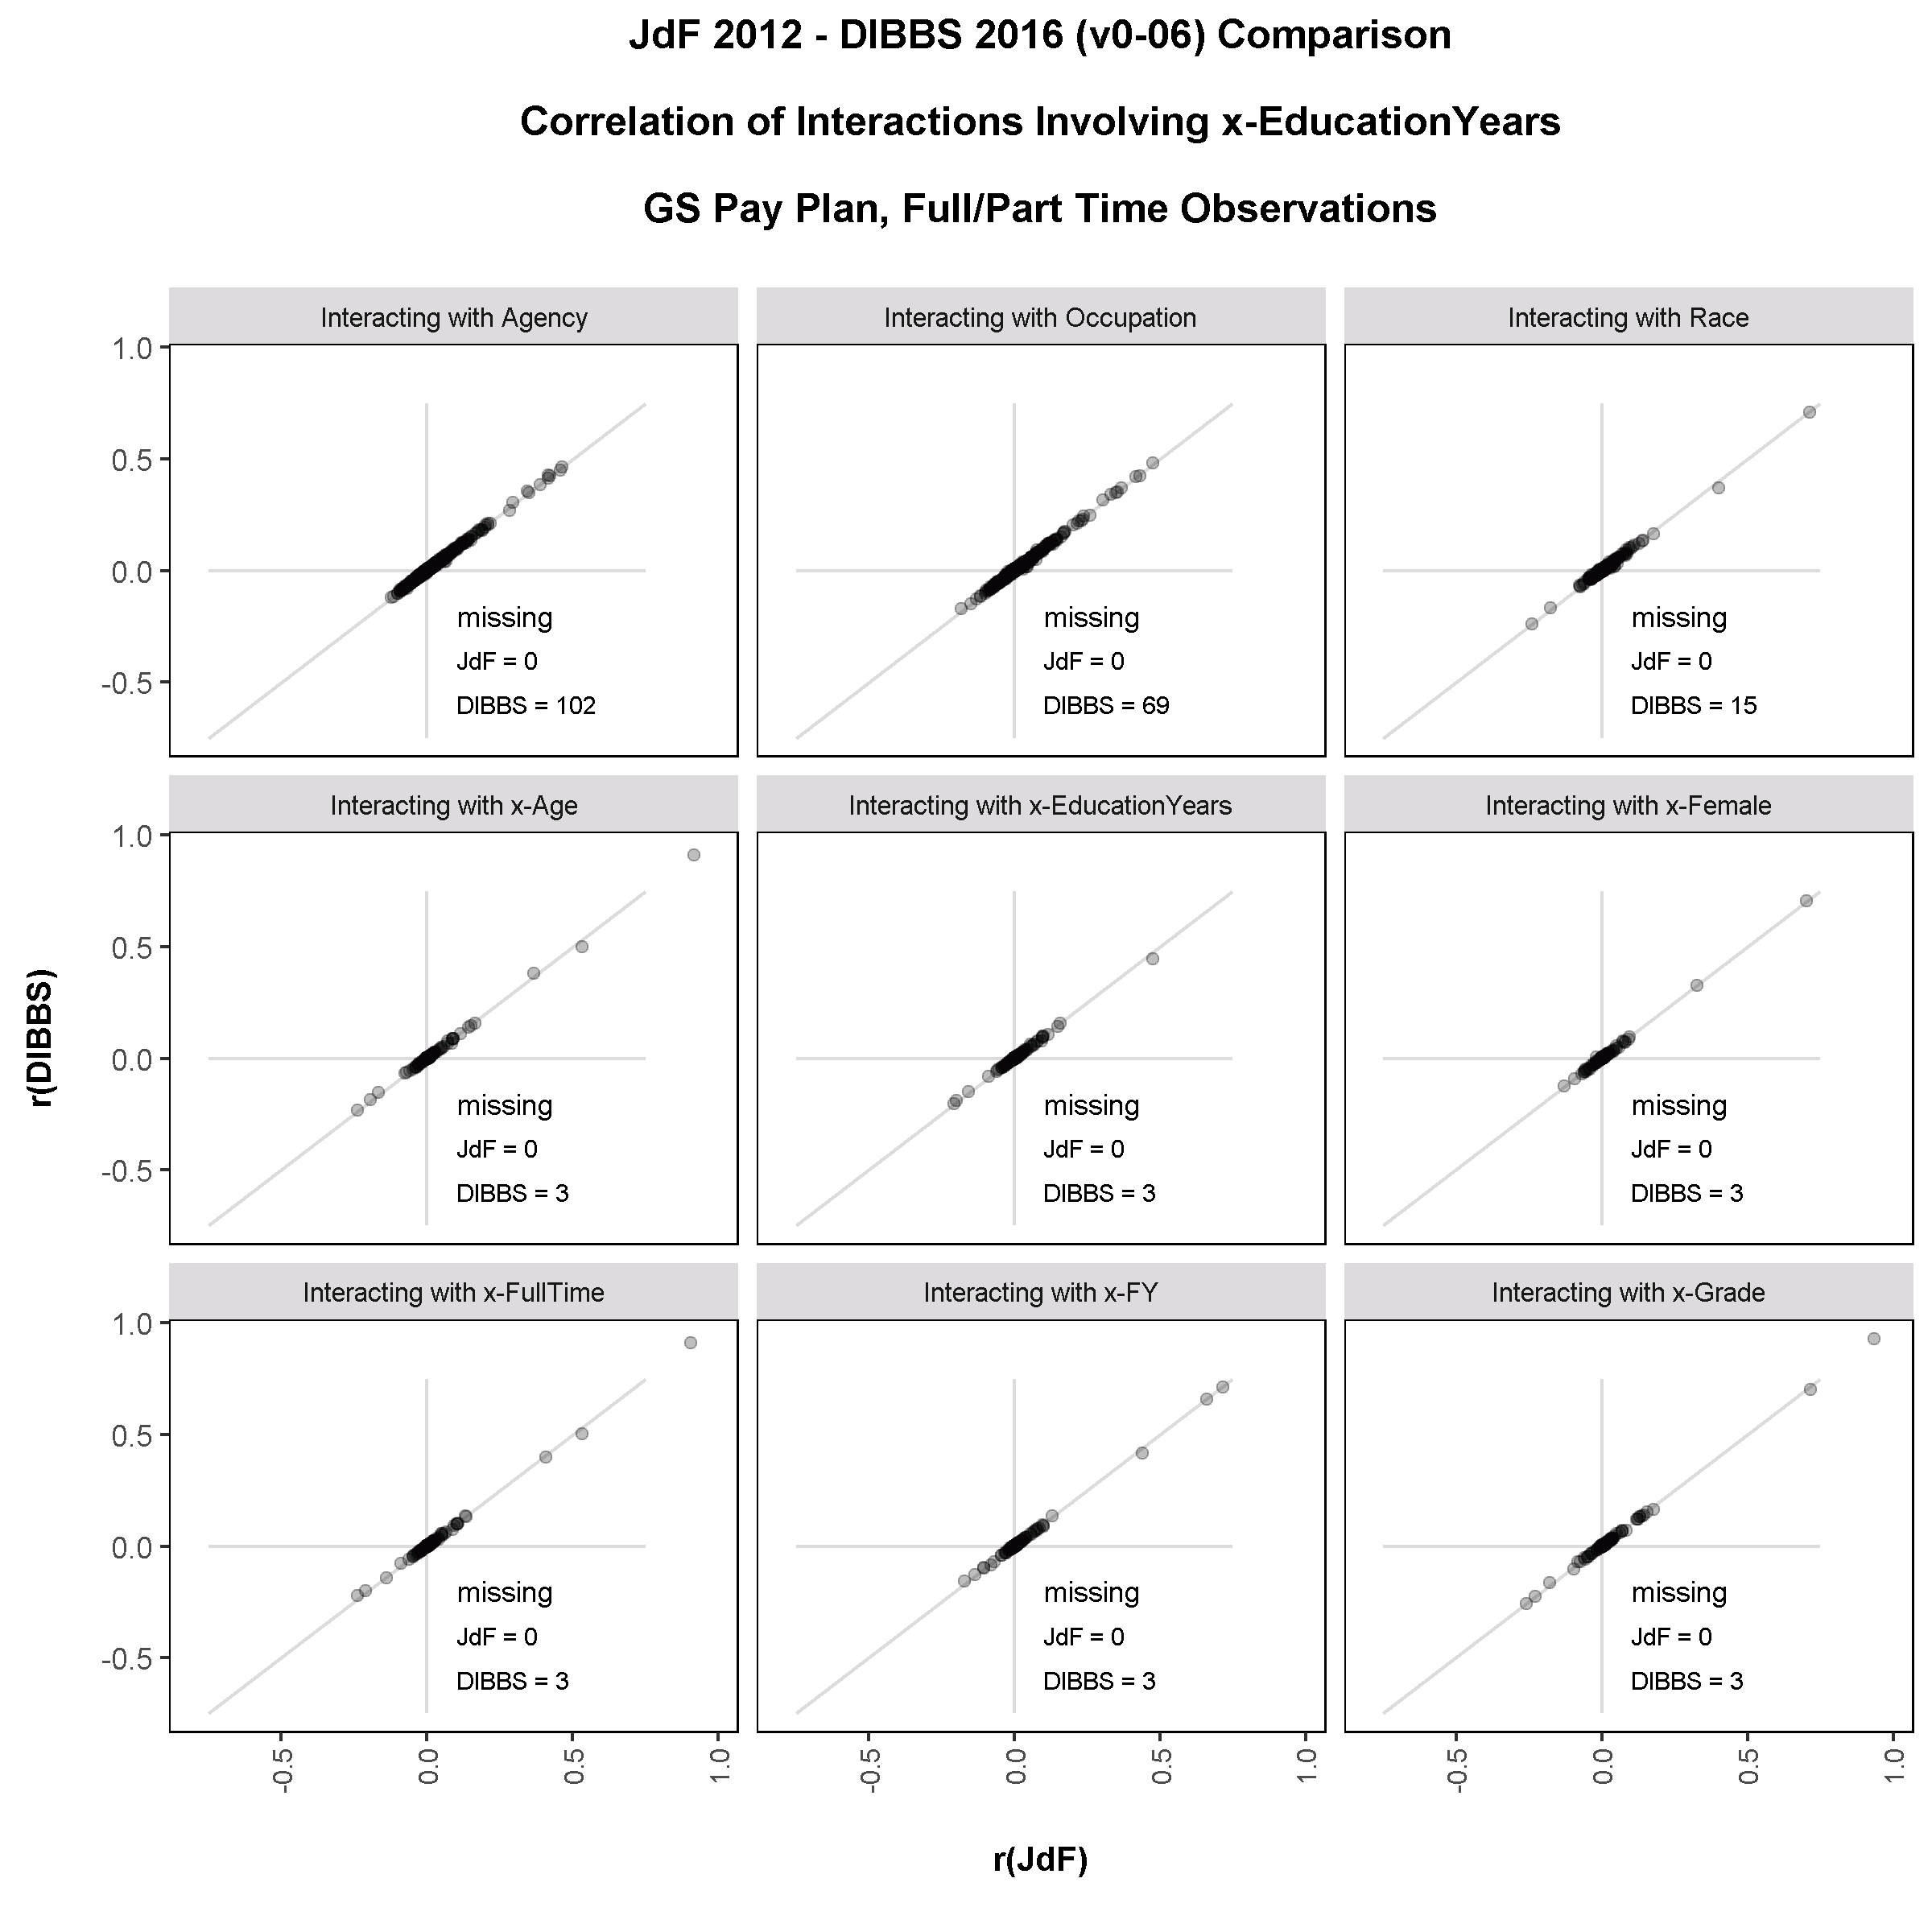
\includegraphics[width=3in, trim={0 0.25in 0 1in}, clip]{JdFDIBBSCorrelationInteraction-x-EducationYears.png}
        \caption{Correlations involving Education}
        %\label{figure:}
        \vspace{10pt}
    \end{subfigure}
    \begin{subfigure}{.5\textwidth}
        \centering
        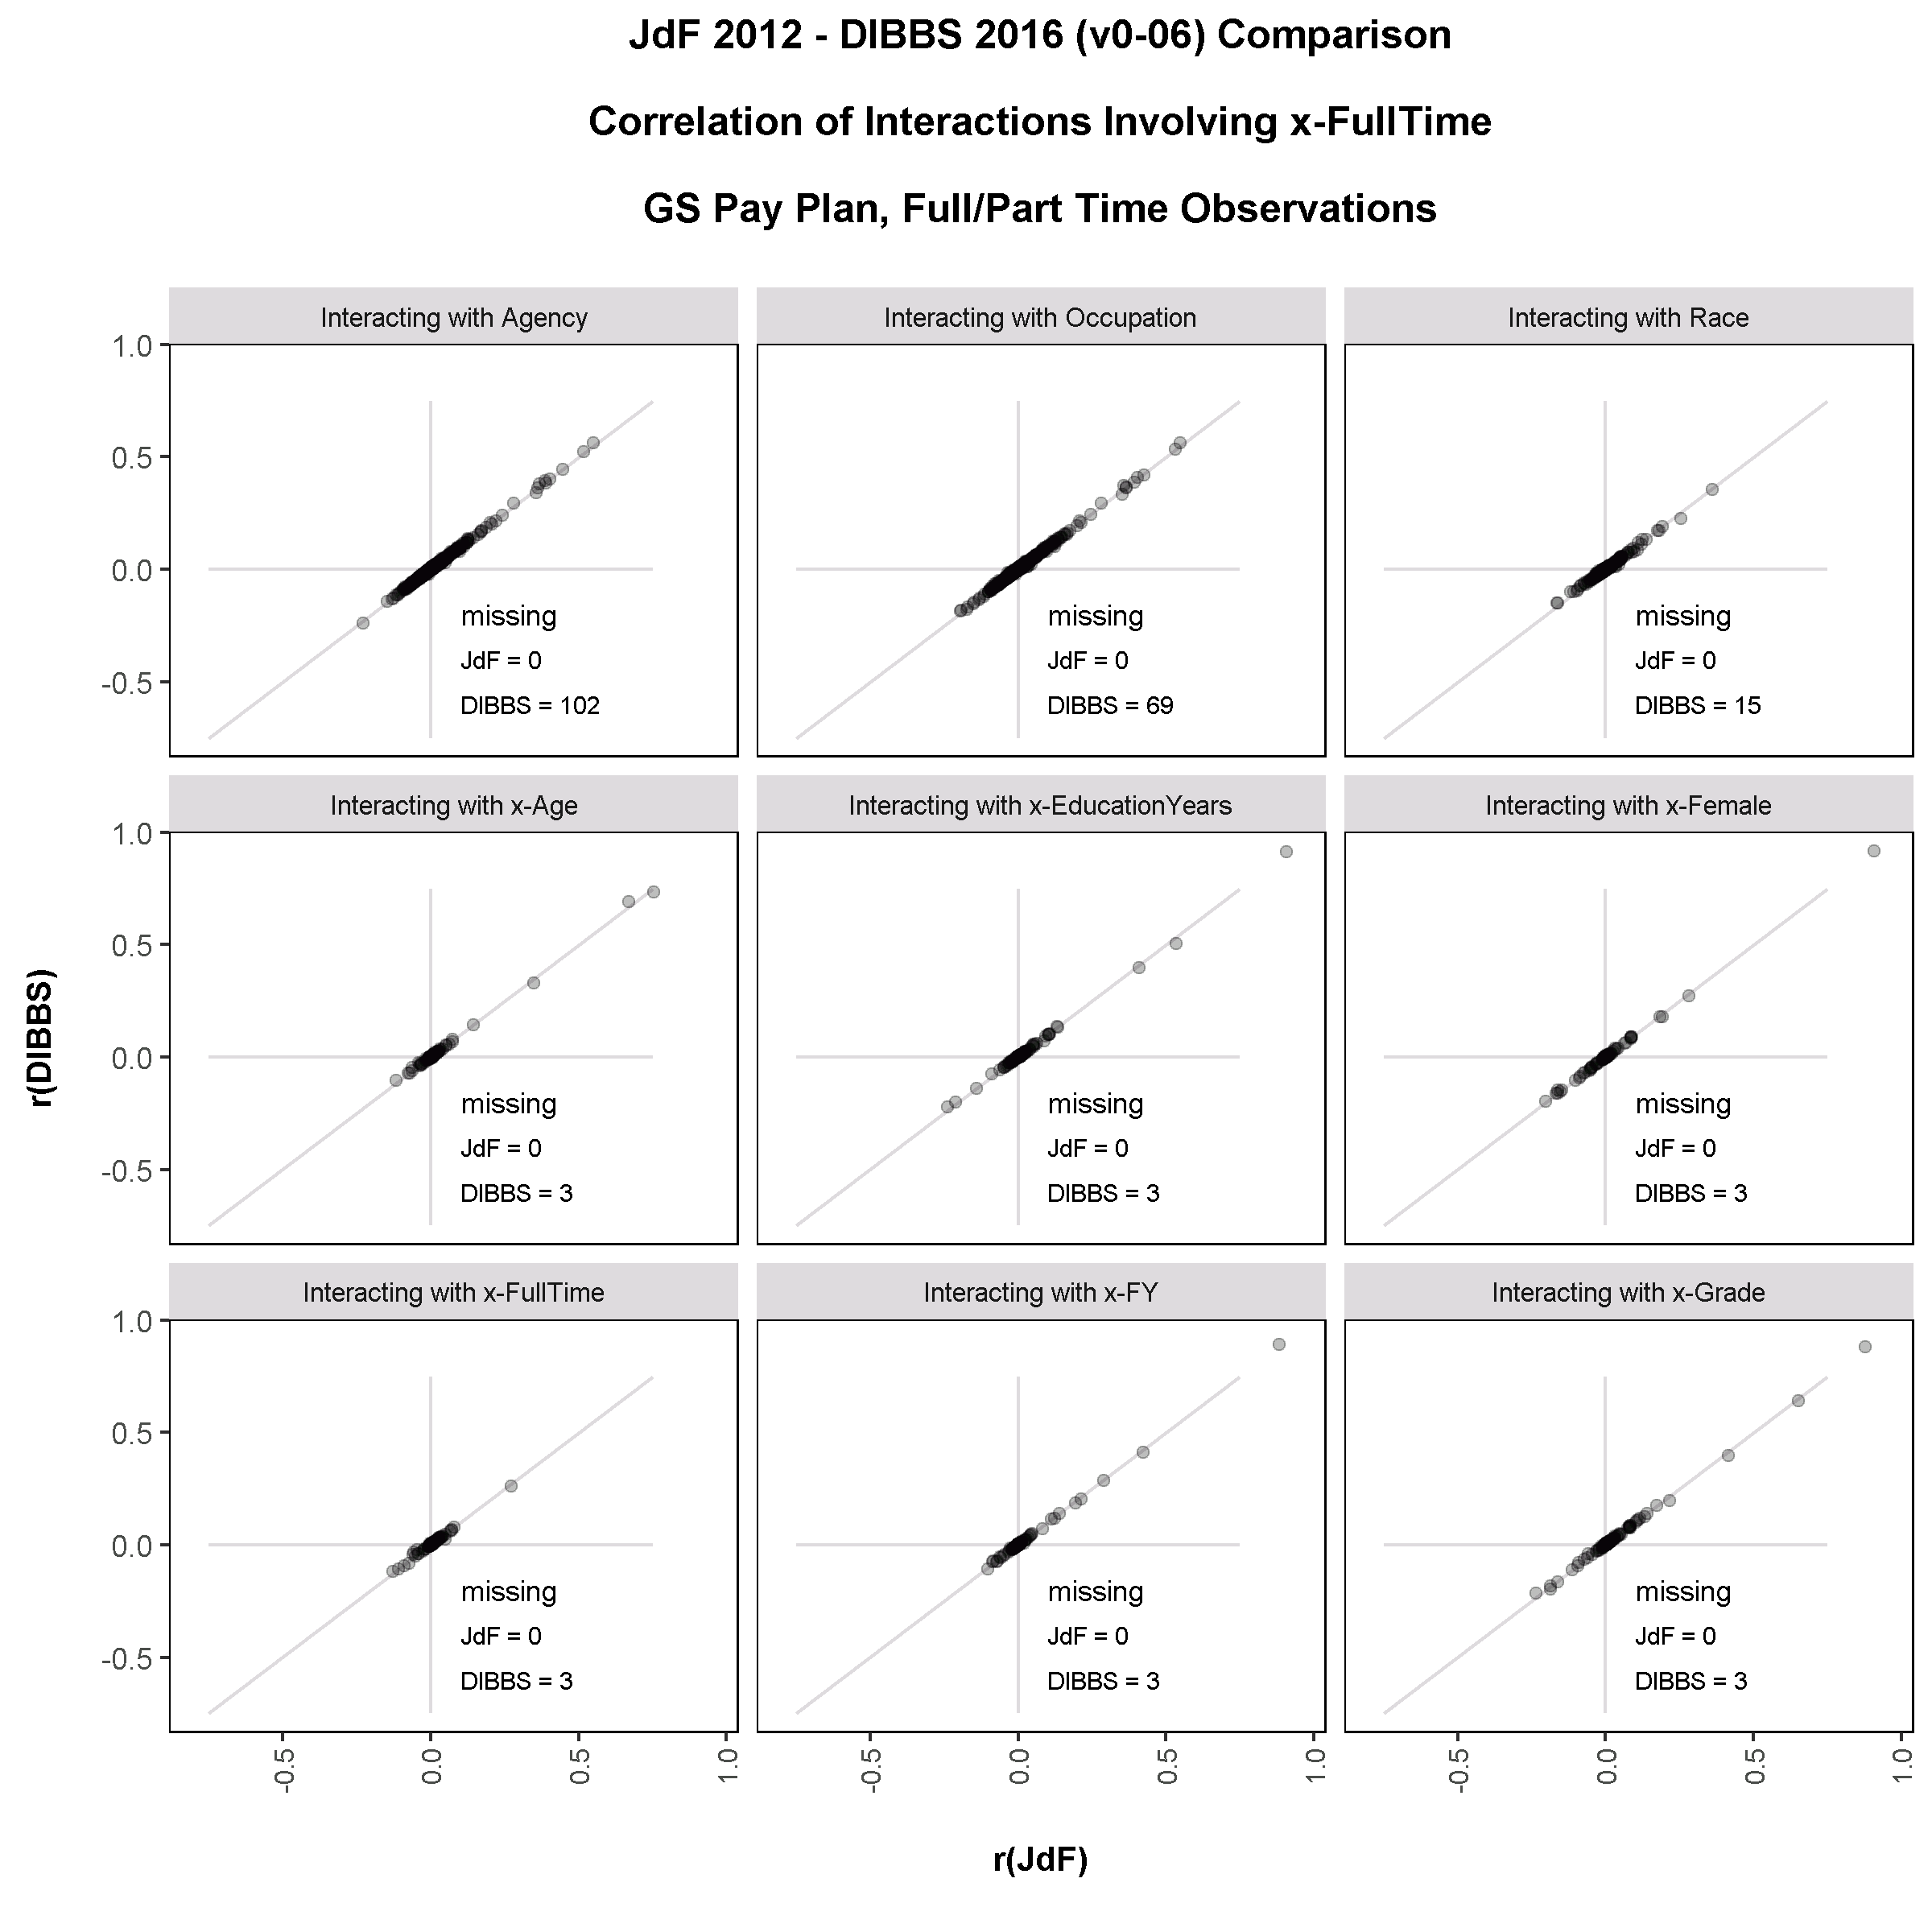
\includegraphics[width=3in, trim={0 0.25in 0 1in}, clip]{JdFDIBBSCorrelationInteraction-x-FullTime.png}
        \caption{Correlations involving Work Schedule}
        %\label{figure:}
        \vspace{10pt}
    \end{subfigure}
    \caption{Correlations of primary variables with two variable interactions.  Variable set two.  Synthetic level correlation on y-axis, corresponding authentic correlation on x-axis.}
    \label{figure:JdFDIBBSCorrelationInteraction2}
\end{figure}  

\clearpage

CUMULATIVE MASS (PROPORTION OBSERVATIONS) BY PAY PLAN AND OCCUPATION\\

Figures \ref{figure:CMFOccupationPayPlan1} and \ref{figure:CMFOccupationPayPlan2} contain example CMF plots of pay plan and occupation combinations.  All occupations within each pay plan are represented.  Solid line for authentic data, dashed line for synthetic.  Overlapping or nearness of lines indicates equality of cumulative mass for corresponding levels of occupation within pay plan.  ``nJ" indicates observation count in authentic data, ``nD" indicates synthetic data observation count.  Near identical distribution is observed for high frequency pay plans GS, WG, GM, and VN, which account for more than 95\% of observations, indicating overall close agreement between data sets.  Increasing departure observed as number of observations decreases.\\

\begin{figure}[h!]
    \centering
    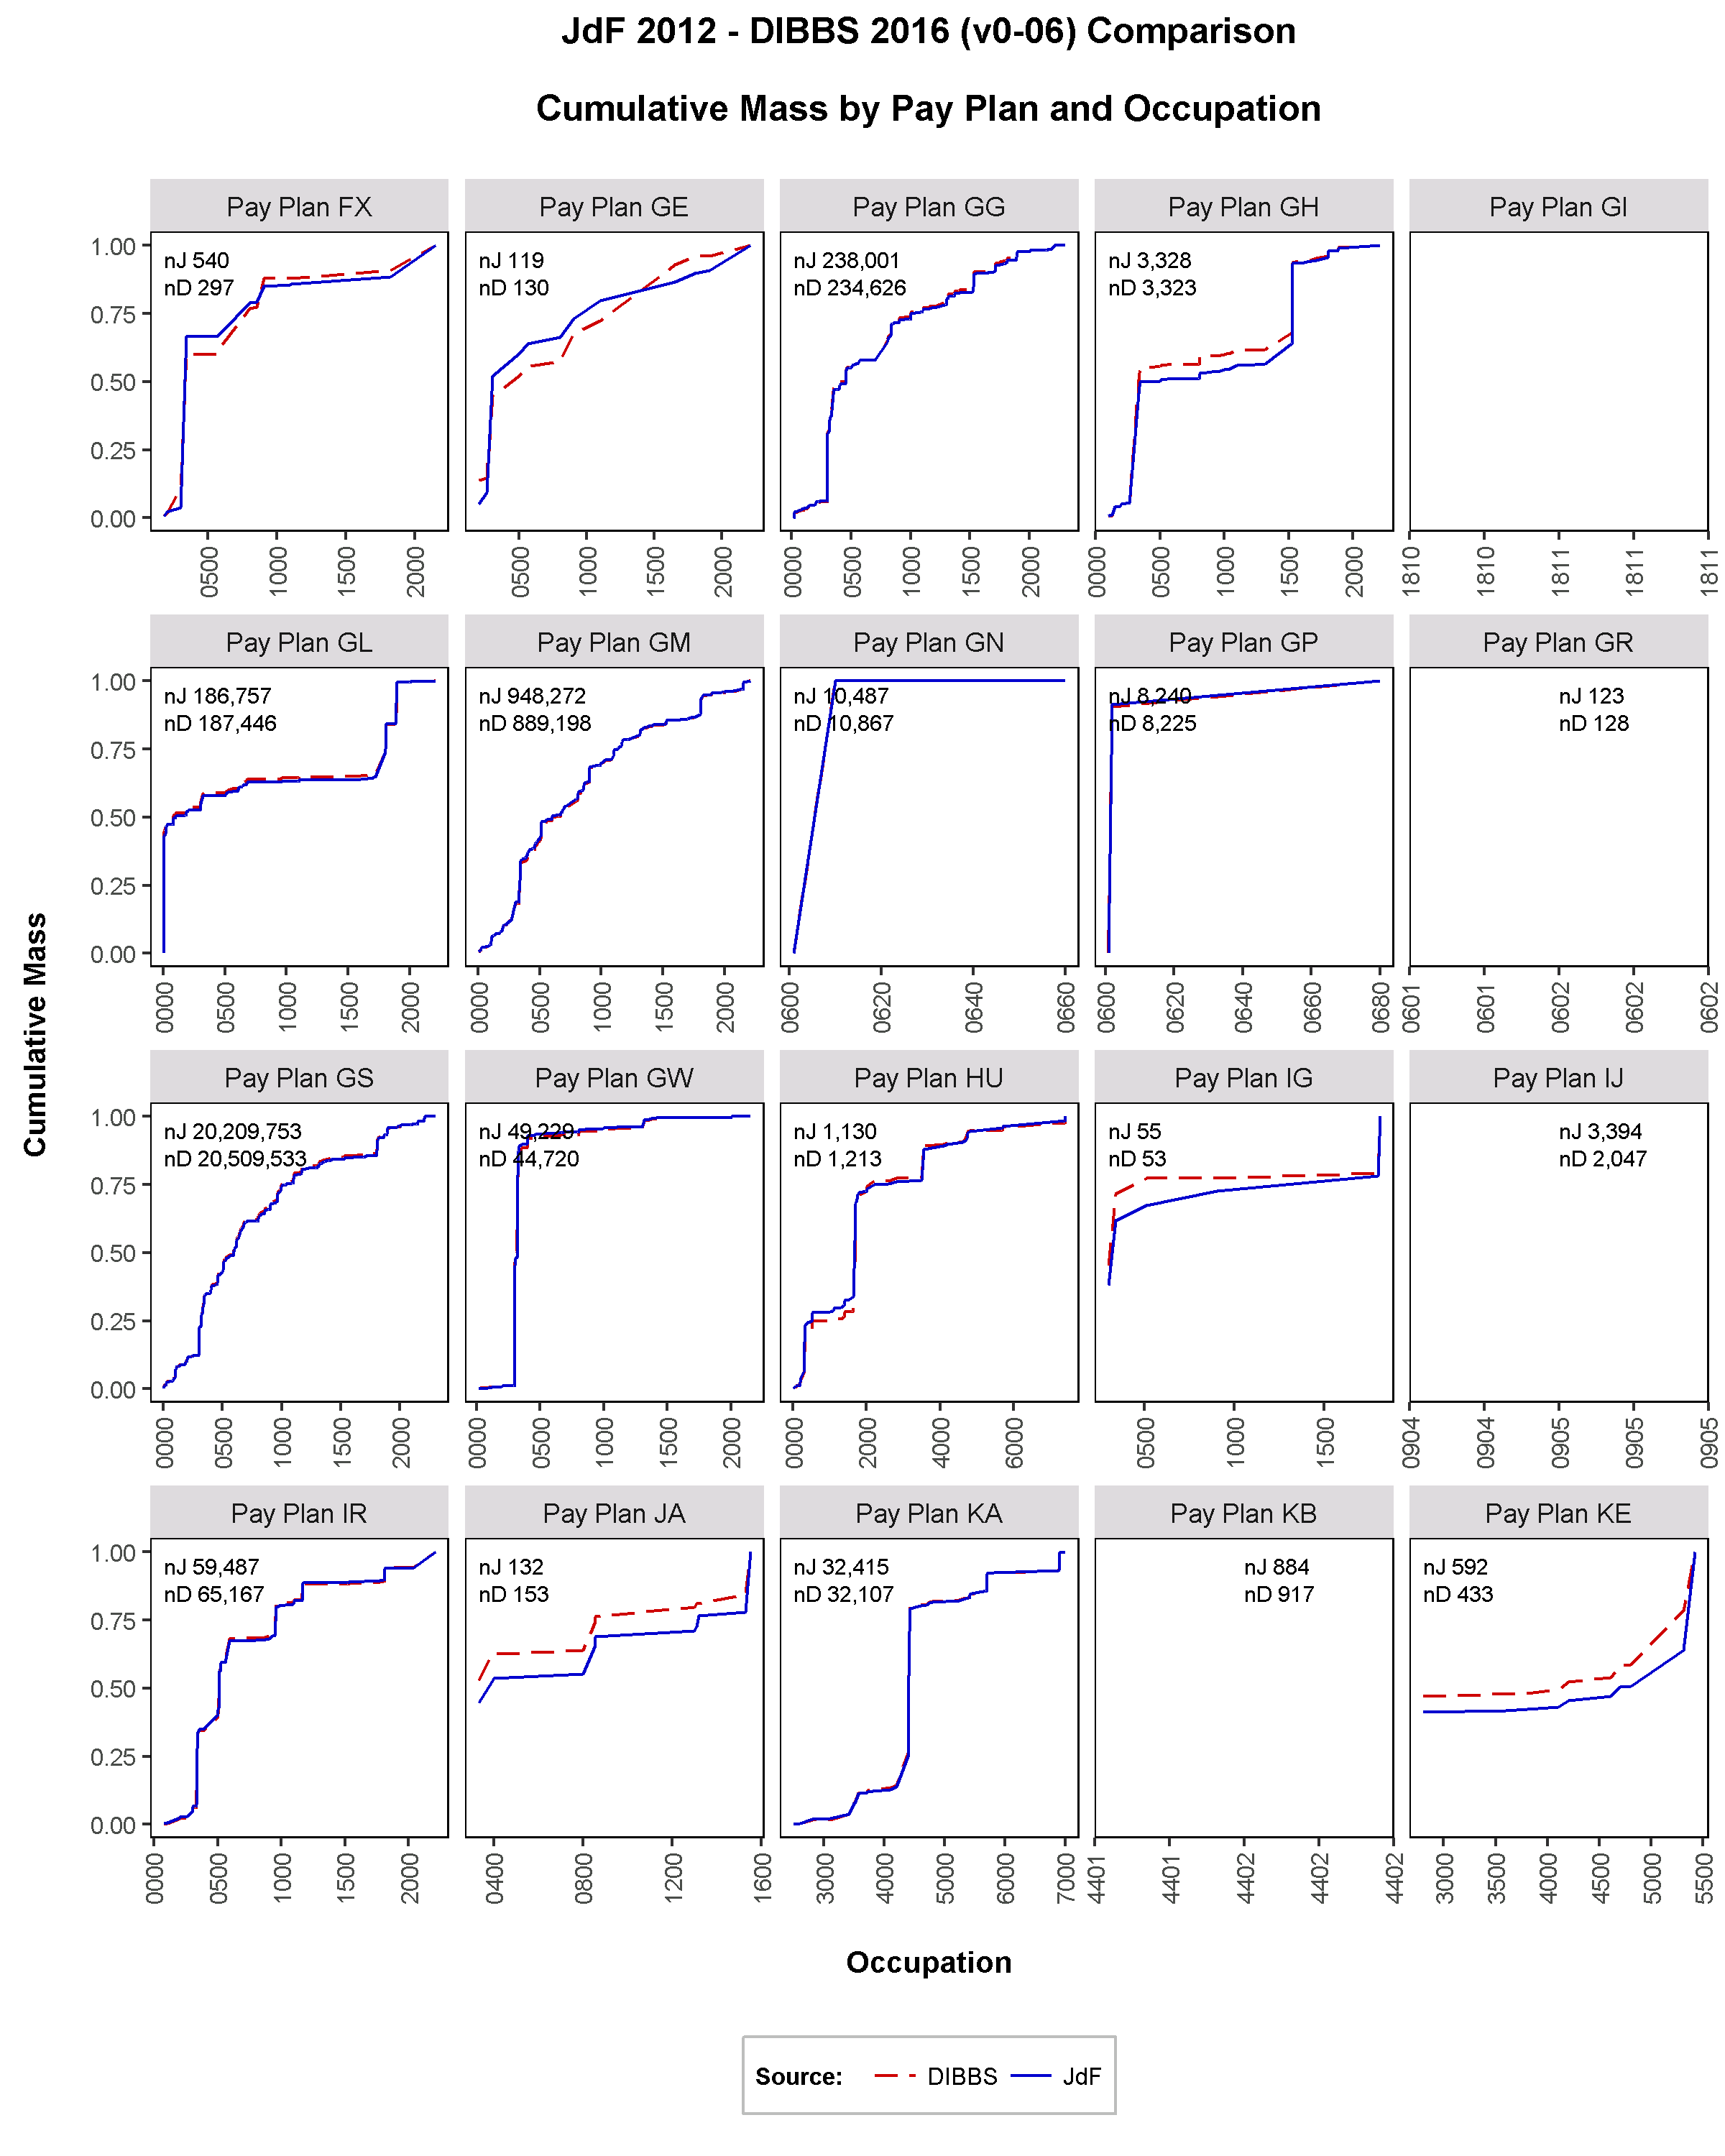
\includegraphics[width=5.9in, trim={0 0 0 0.75in}, clip]{CMFOccupationPayPlan61.png}
    \caption{Cumulative mass by occupation within pay plan.  Pay plan set one.}
    \label{figure:CMFOccupationPayPlan1}
\end{figure}

\begin{figure}[h!]
    \centering
    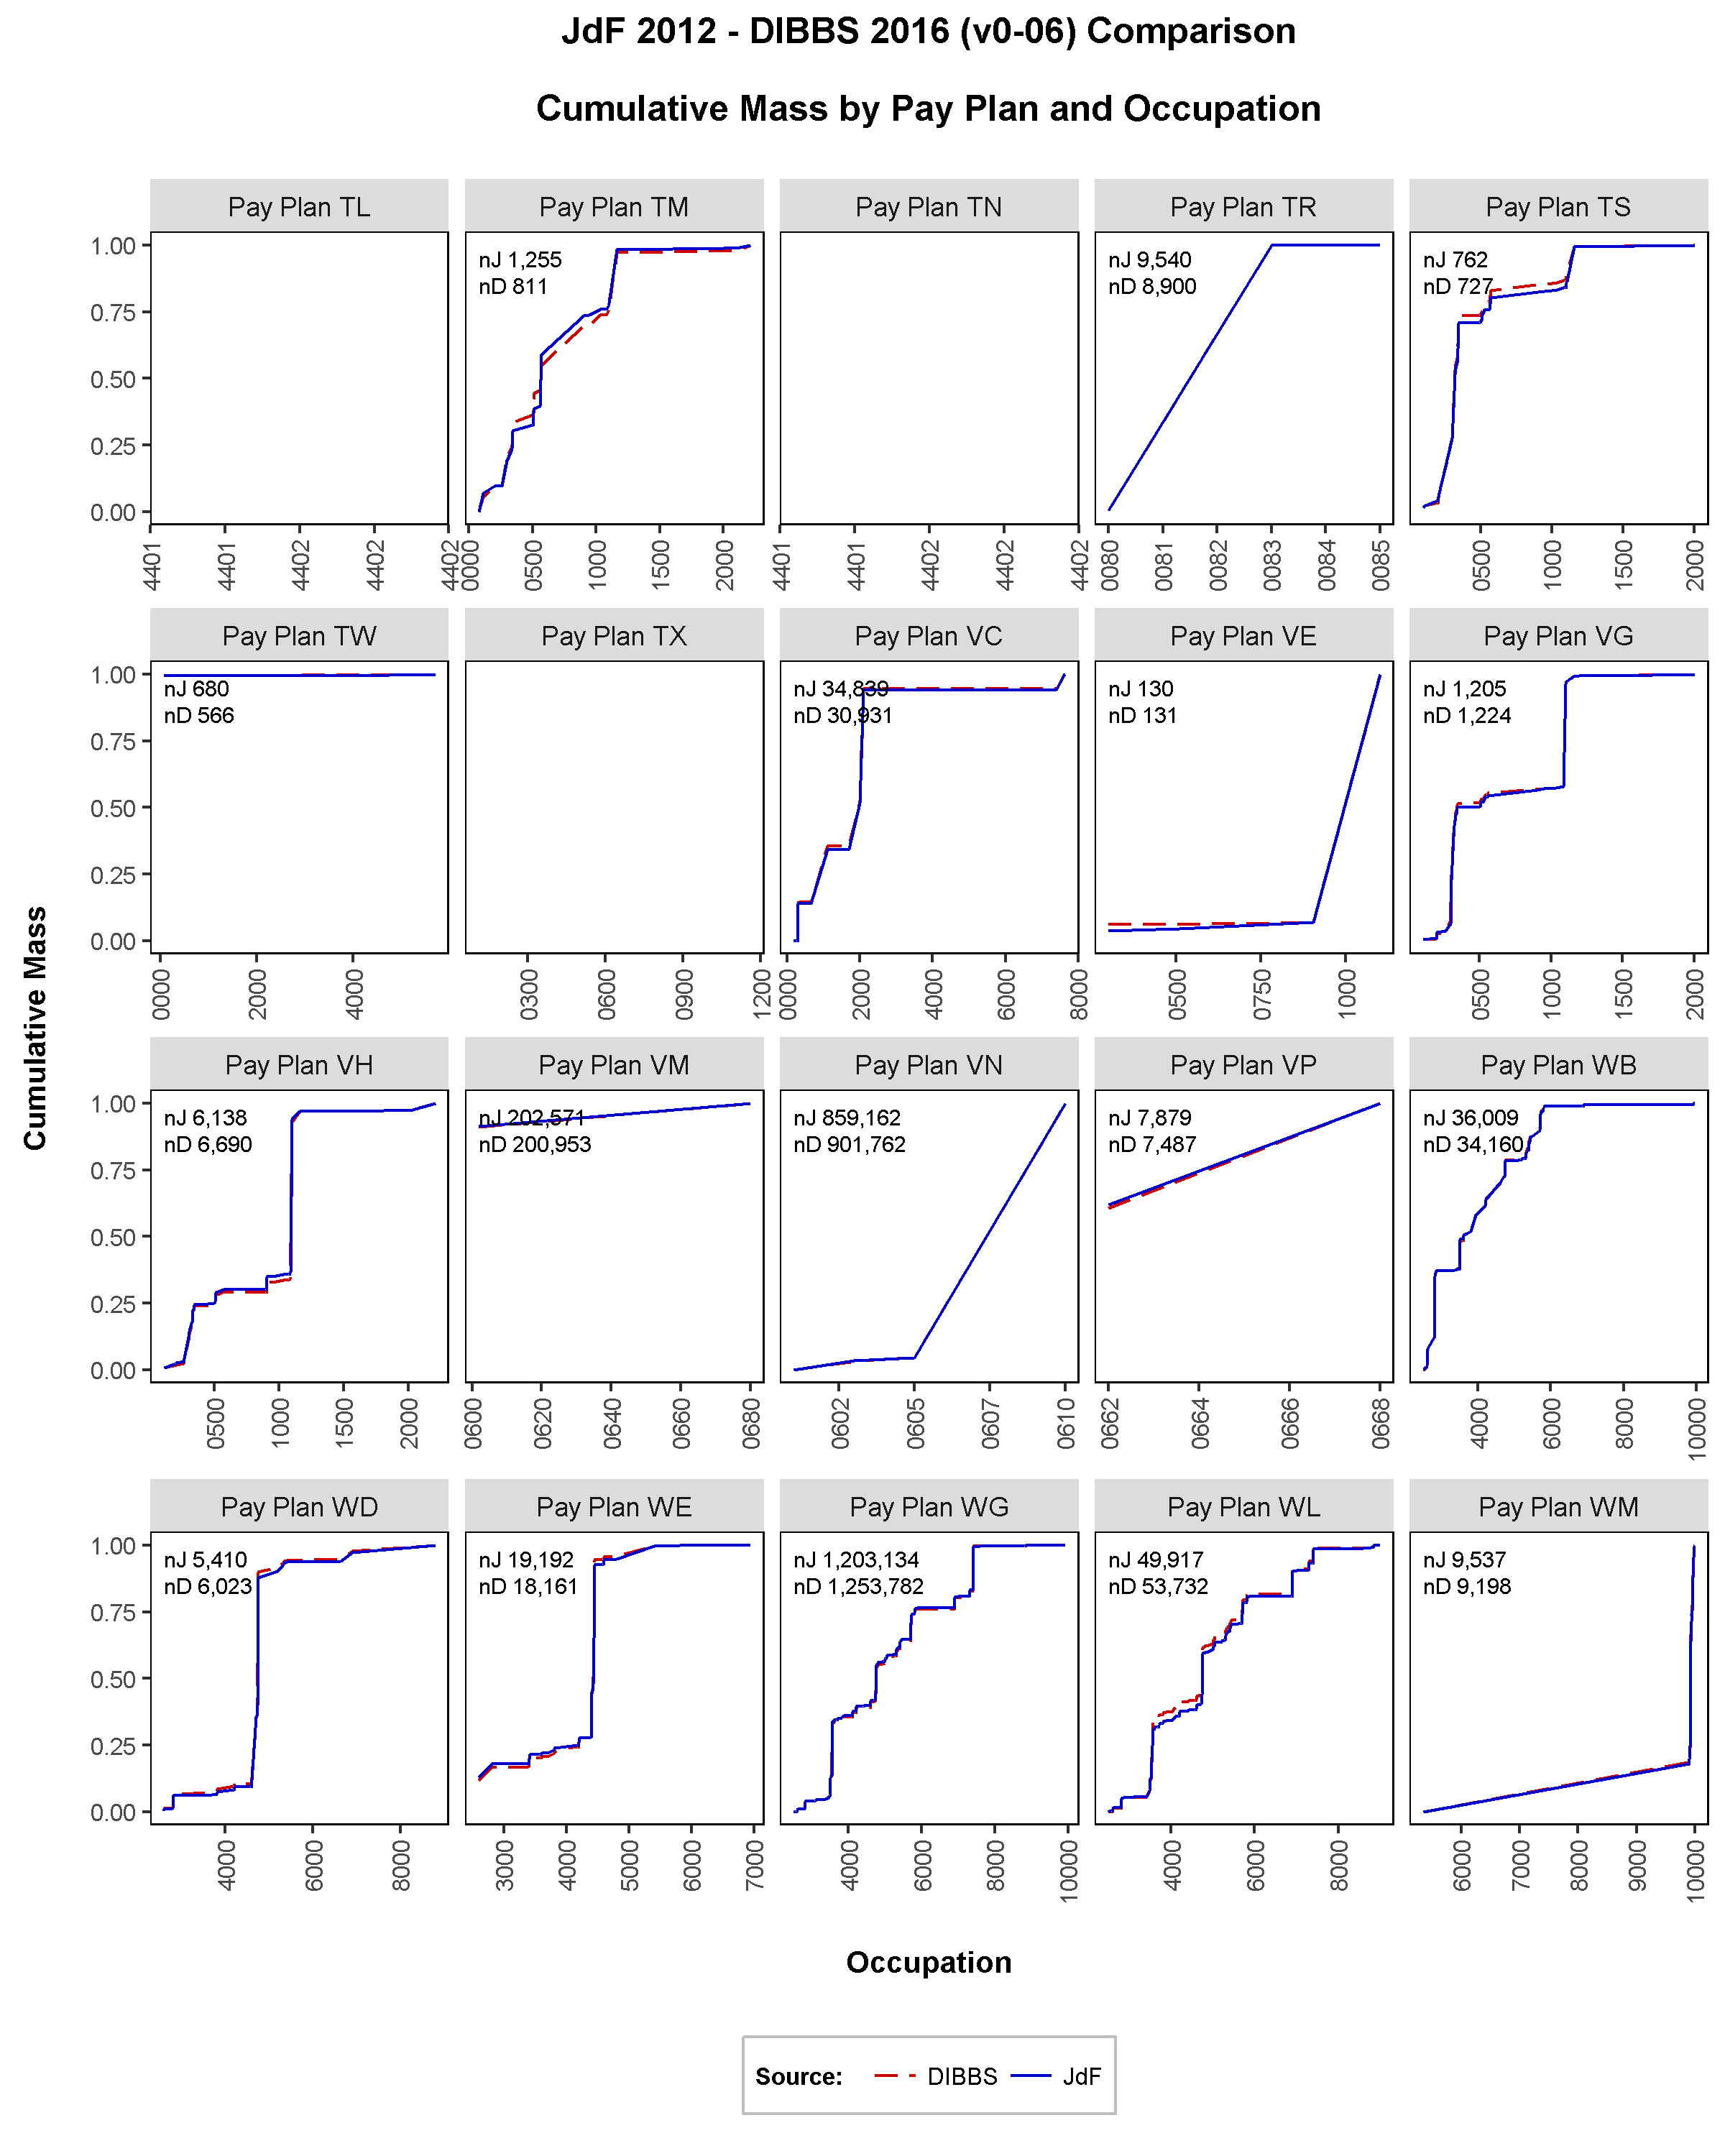
\includegraphics[width=5.9in, trim={0 0 0 0.75in}, clip]{CMFOccupationPayPlan141.png}
    \caption{Cumulative mass by occupation within pay plan.  Pay plan set 2.}
    \label{figure:CMFOccupationPayPlan2}
\end{figure}

\clearpage

DISTRIBUTION OF BASIC PAY BY AGENCY\\

Basic pay is an important dependent study variable and the distribution of pay values in the authentic data must be maintained in the synthetic data.  Figure \ref{figure:JdFDIBBSBasicPayDistribution} plots the distribution of basic pay for the top eight frequency agencies (first two positions):  Department of Agriculture (AG), Department of Justice (DJ), Department of Health and Human Services (HE), Department of Homeland Security (HS), Department of Interior (IN), Department of Transportation (TD), Department of Treasury (TR), and the Department of Veterans Affairs (VA).  These agencies account for approximately 85\% of observations.  Synthetic distribution represented by dashed line, authentic distribution by solid line.  ``n(D)" indicates synthetic data observation frequency, ``n(J)" indicates authentic data observation count.\\

Observations:  Although each data set is represented in each graph, a single striped-appearing line is visible, due to identical frequency proportions at each pay level.  Local increases, decreases, and trends in authentic distribution are accurately represented in the synthetic data.\\

\begin{figure}[h!]
    \centering
    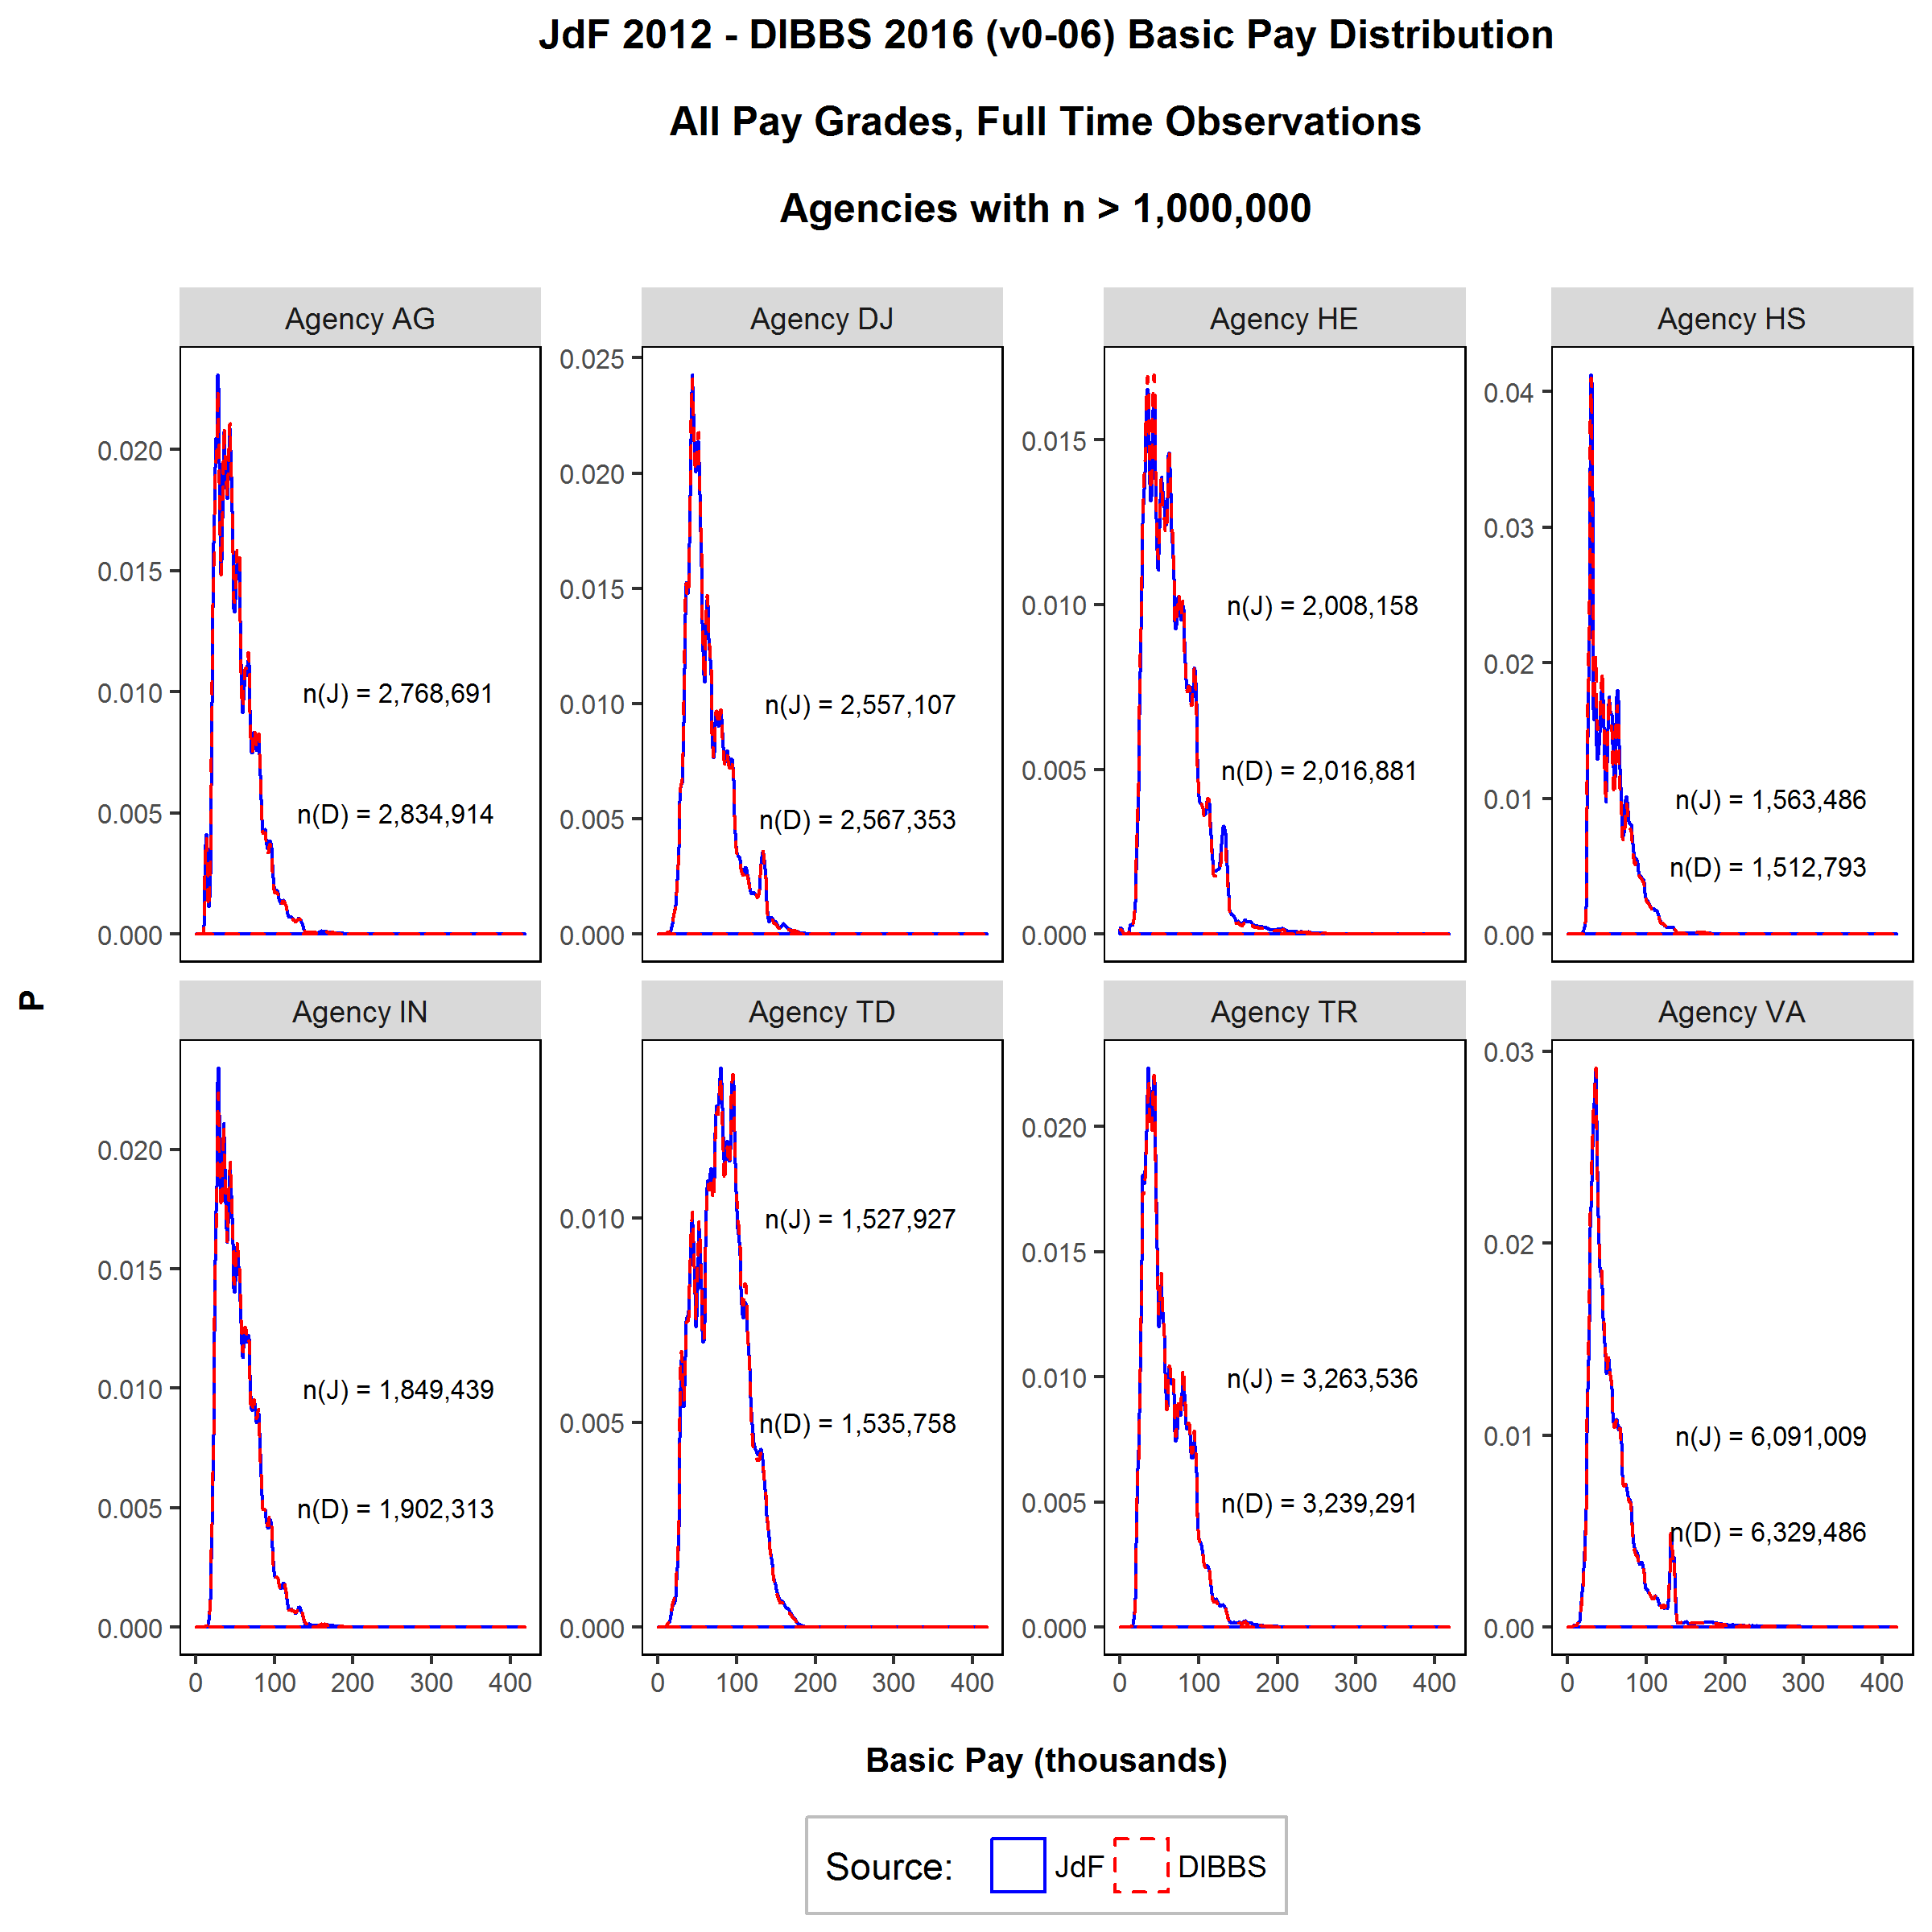
\includegraphics[width=4.5in, trim={0 0 1in 1in}, clip]{JdFDIBBSBasicPayDistribution.png}
    \caption{Basic pay marginal distribution for top eight agencies.  Dashed line for synthetic data, solid line for authentic.}
    \label{figure:JdFDIBBSBasicPayDistribution}
\end{figure}

\clearpage

DISTRIBUTION OF BASIC PAY BY PROFESSIONAL, SUPERVISORY, COLLEGE EDUCATION, AND WORK SCHEDULE CATEGORY\\

Professional classification, supervisory status, and college education are important independent variables in human capital research.  Figures \ref{figure:JdFDIBBSBasicPayCDFAG} through \ref{figure:JdFDIBBSBasicPayCDFVA} plot, for the top eight frequency agencies, the distribution of basic pay by these independent variables and work schedule code.  One column for each professional, supervisory, college combination (column code position one equals ``P" if occupational category is administrative or professional, position two equals ``S" if supervisory status is enabled, position three equals ``C" if education level at or above college).  One row for each work schedule code [significant codes are full time (F), full time seasonal (G), intermittent (I), intermittent seasonal (J), and part time (P)].  Synthetic distribution indicated by dashed line, authentic distribution by solid line.  ``n(D)" indicates synthetic data observation frequency, ``n(J)" indicates authentic data observation count.\\

Observations:  There exists near identical distribution for high frequency combinations, as indicated by striped, single line appearance due to overlay of synthetic on authentic lines.  Slight differences in distribution are observed for small frequency combinations.

\vspace{12pt}

\begin{figure}[h]
    \centering
    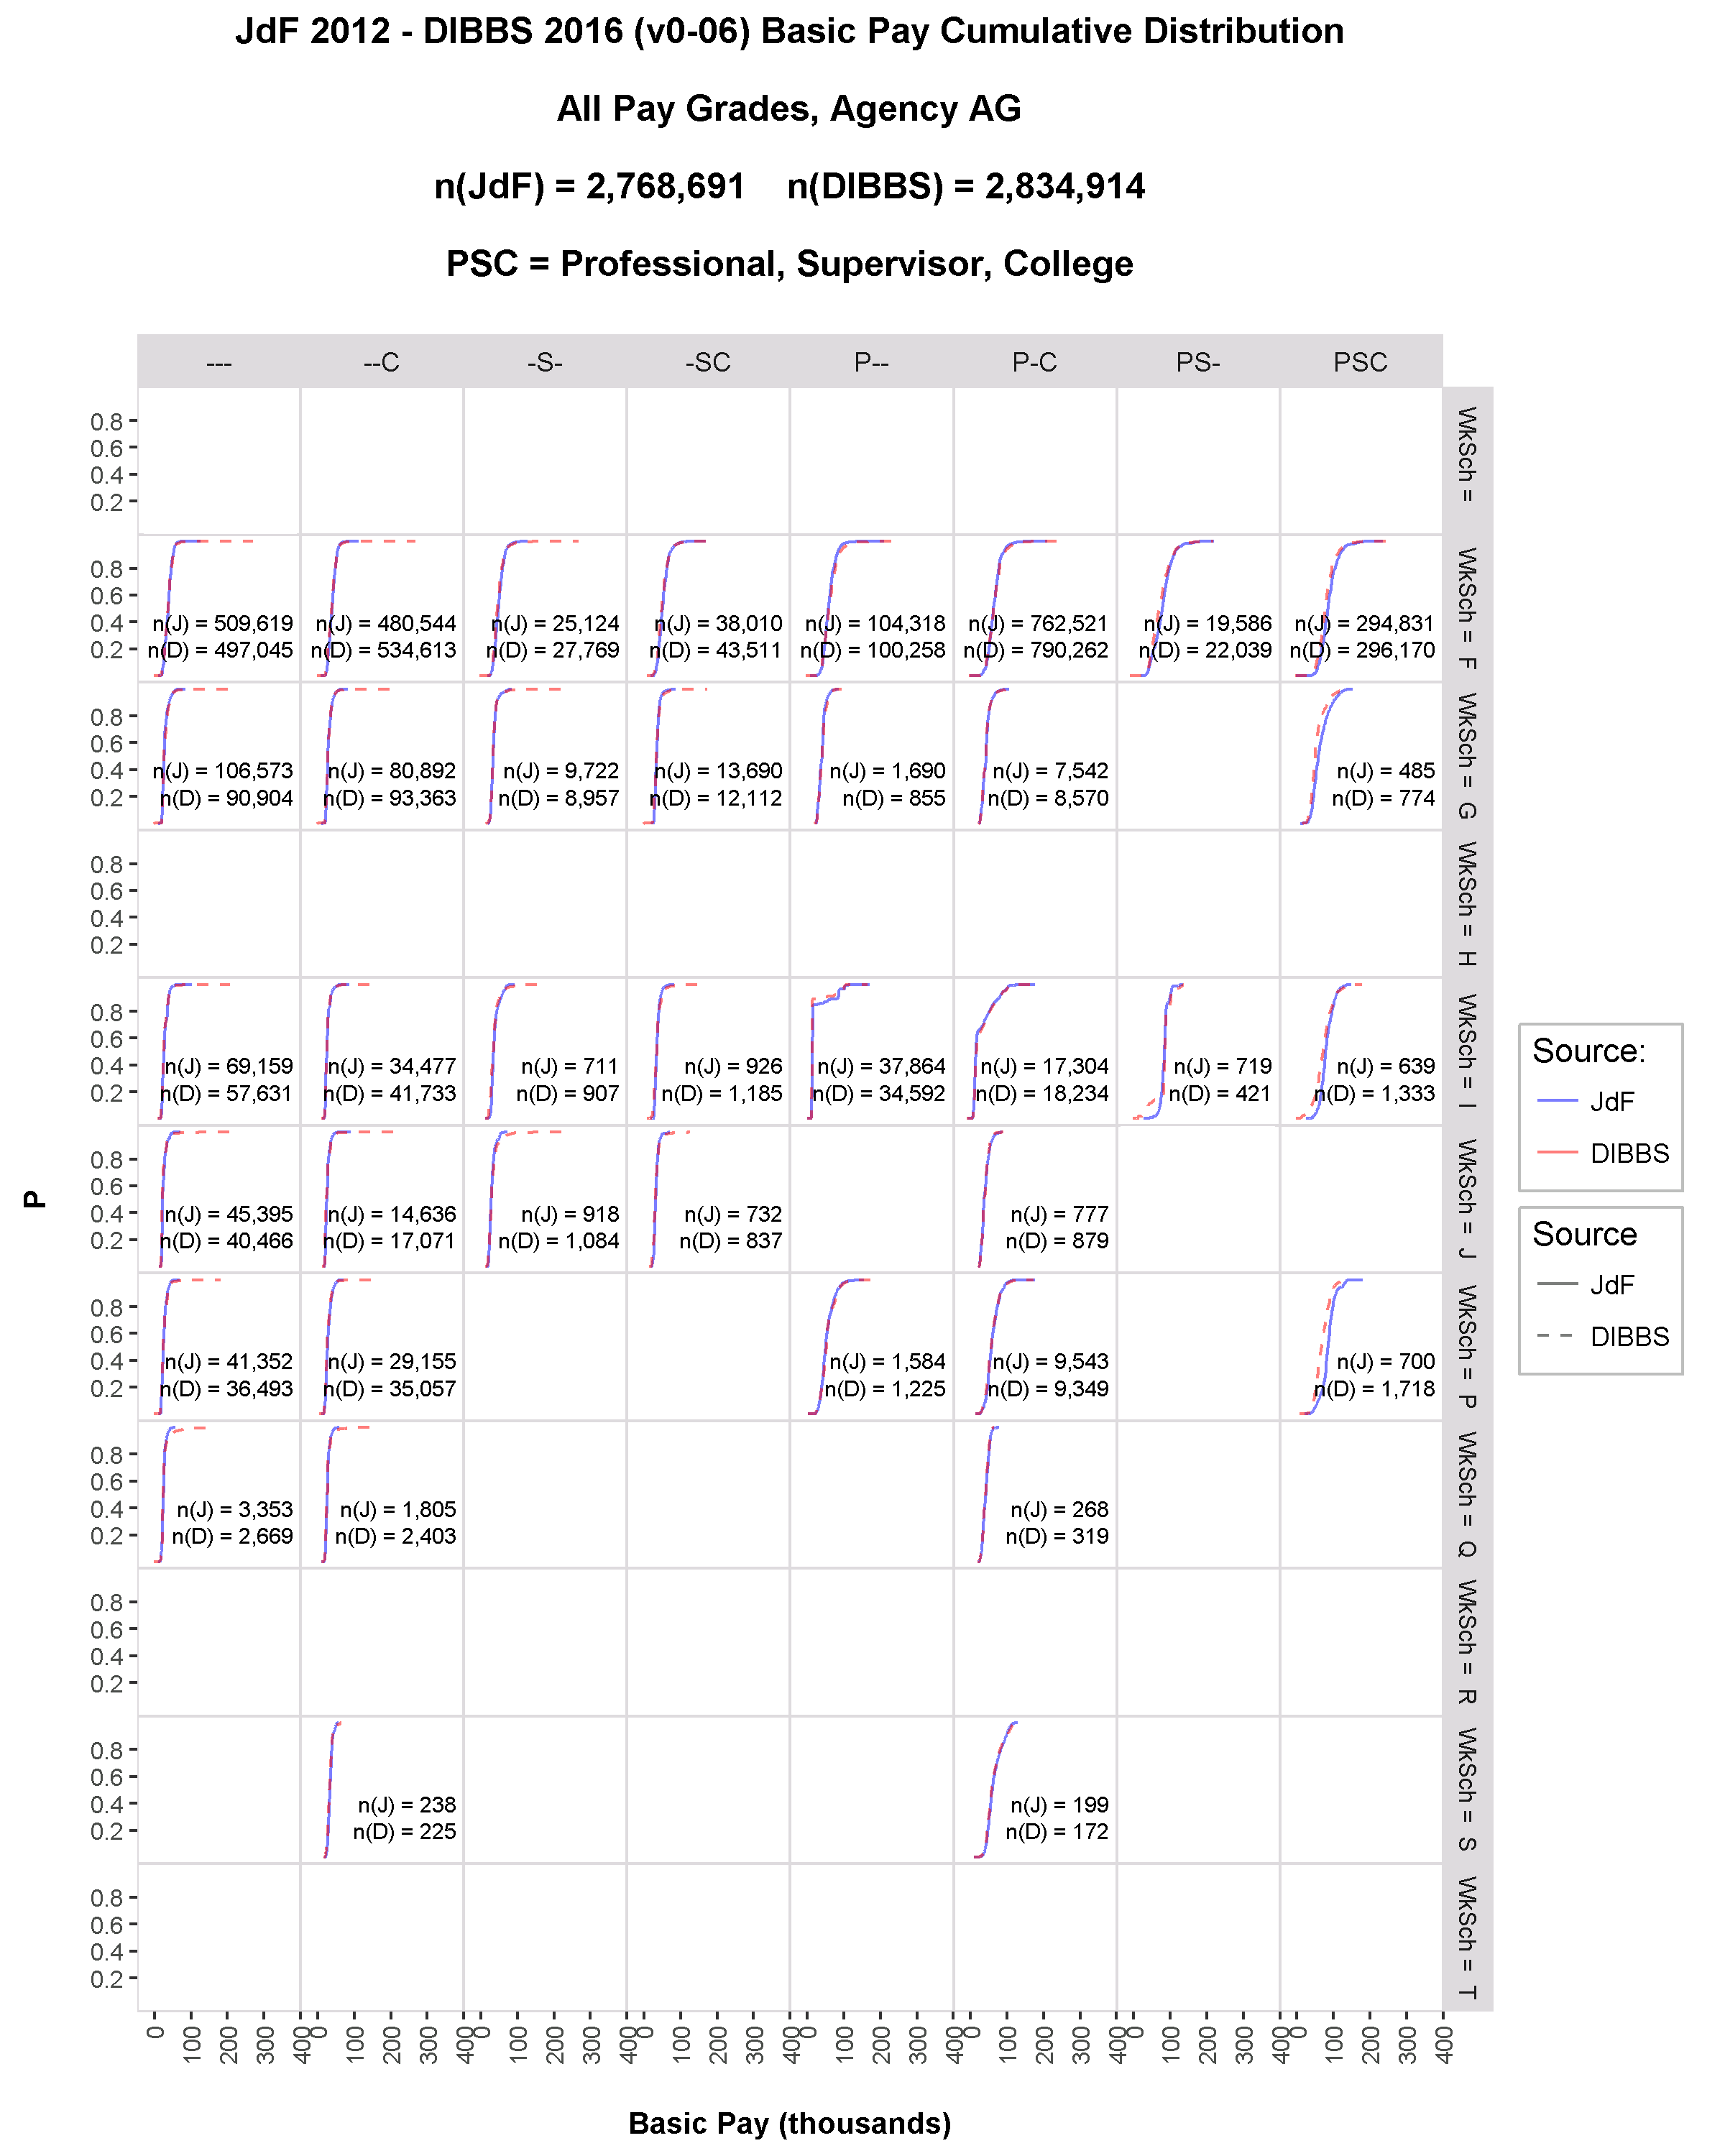
\includegraphics[width=6.5in, trim={0 0 1in 1.5in}, clip]{JdFDIBBSBasicPayCDFAG.png}
    \caption{Basic pay distribution by joint professional, supervisory status, college education, and work schedule  categories.  Department of Agriculture (AG).  Dashed line for synthetic data, solid line for authentic.}
    \label{figure:JdFDIBBSBasicPayCDFAG}
\end{figure}

\clearpage

\begin{figure}[h]
    \centering
    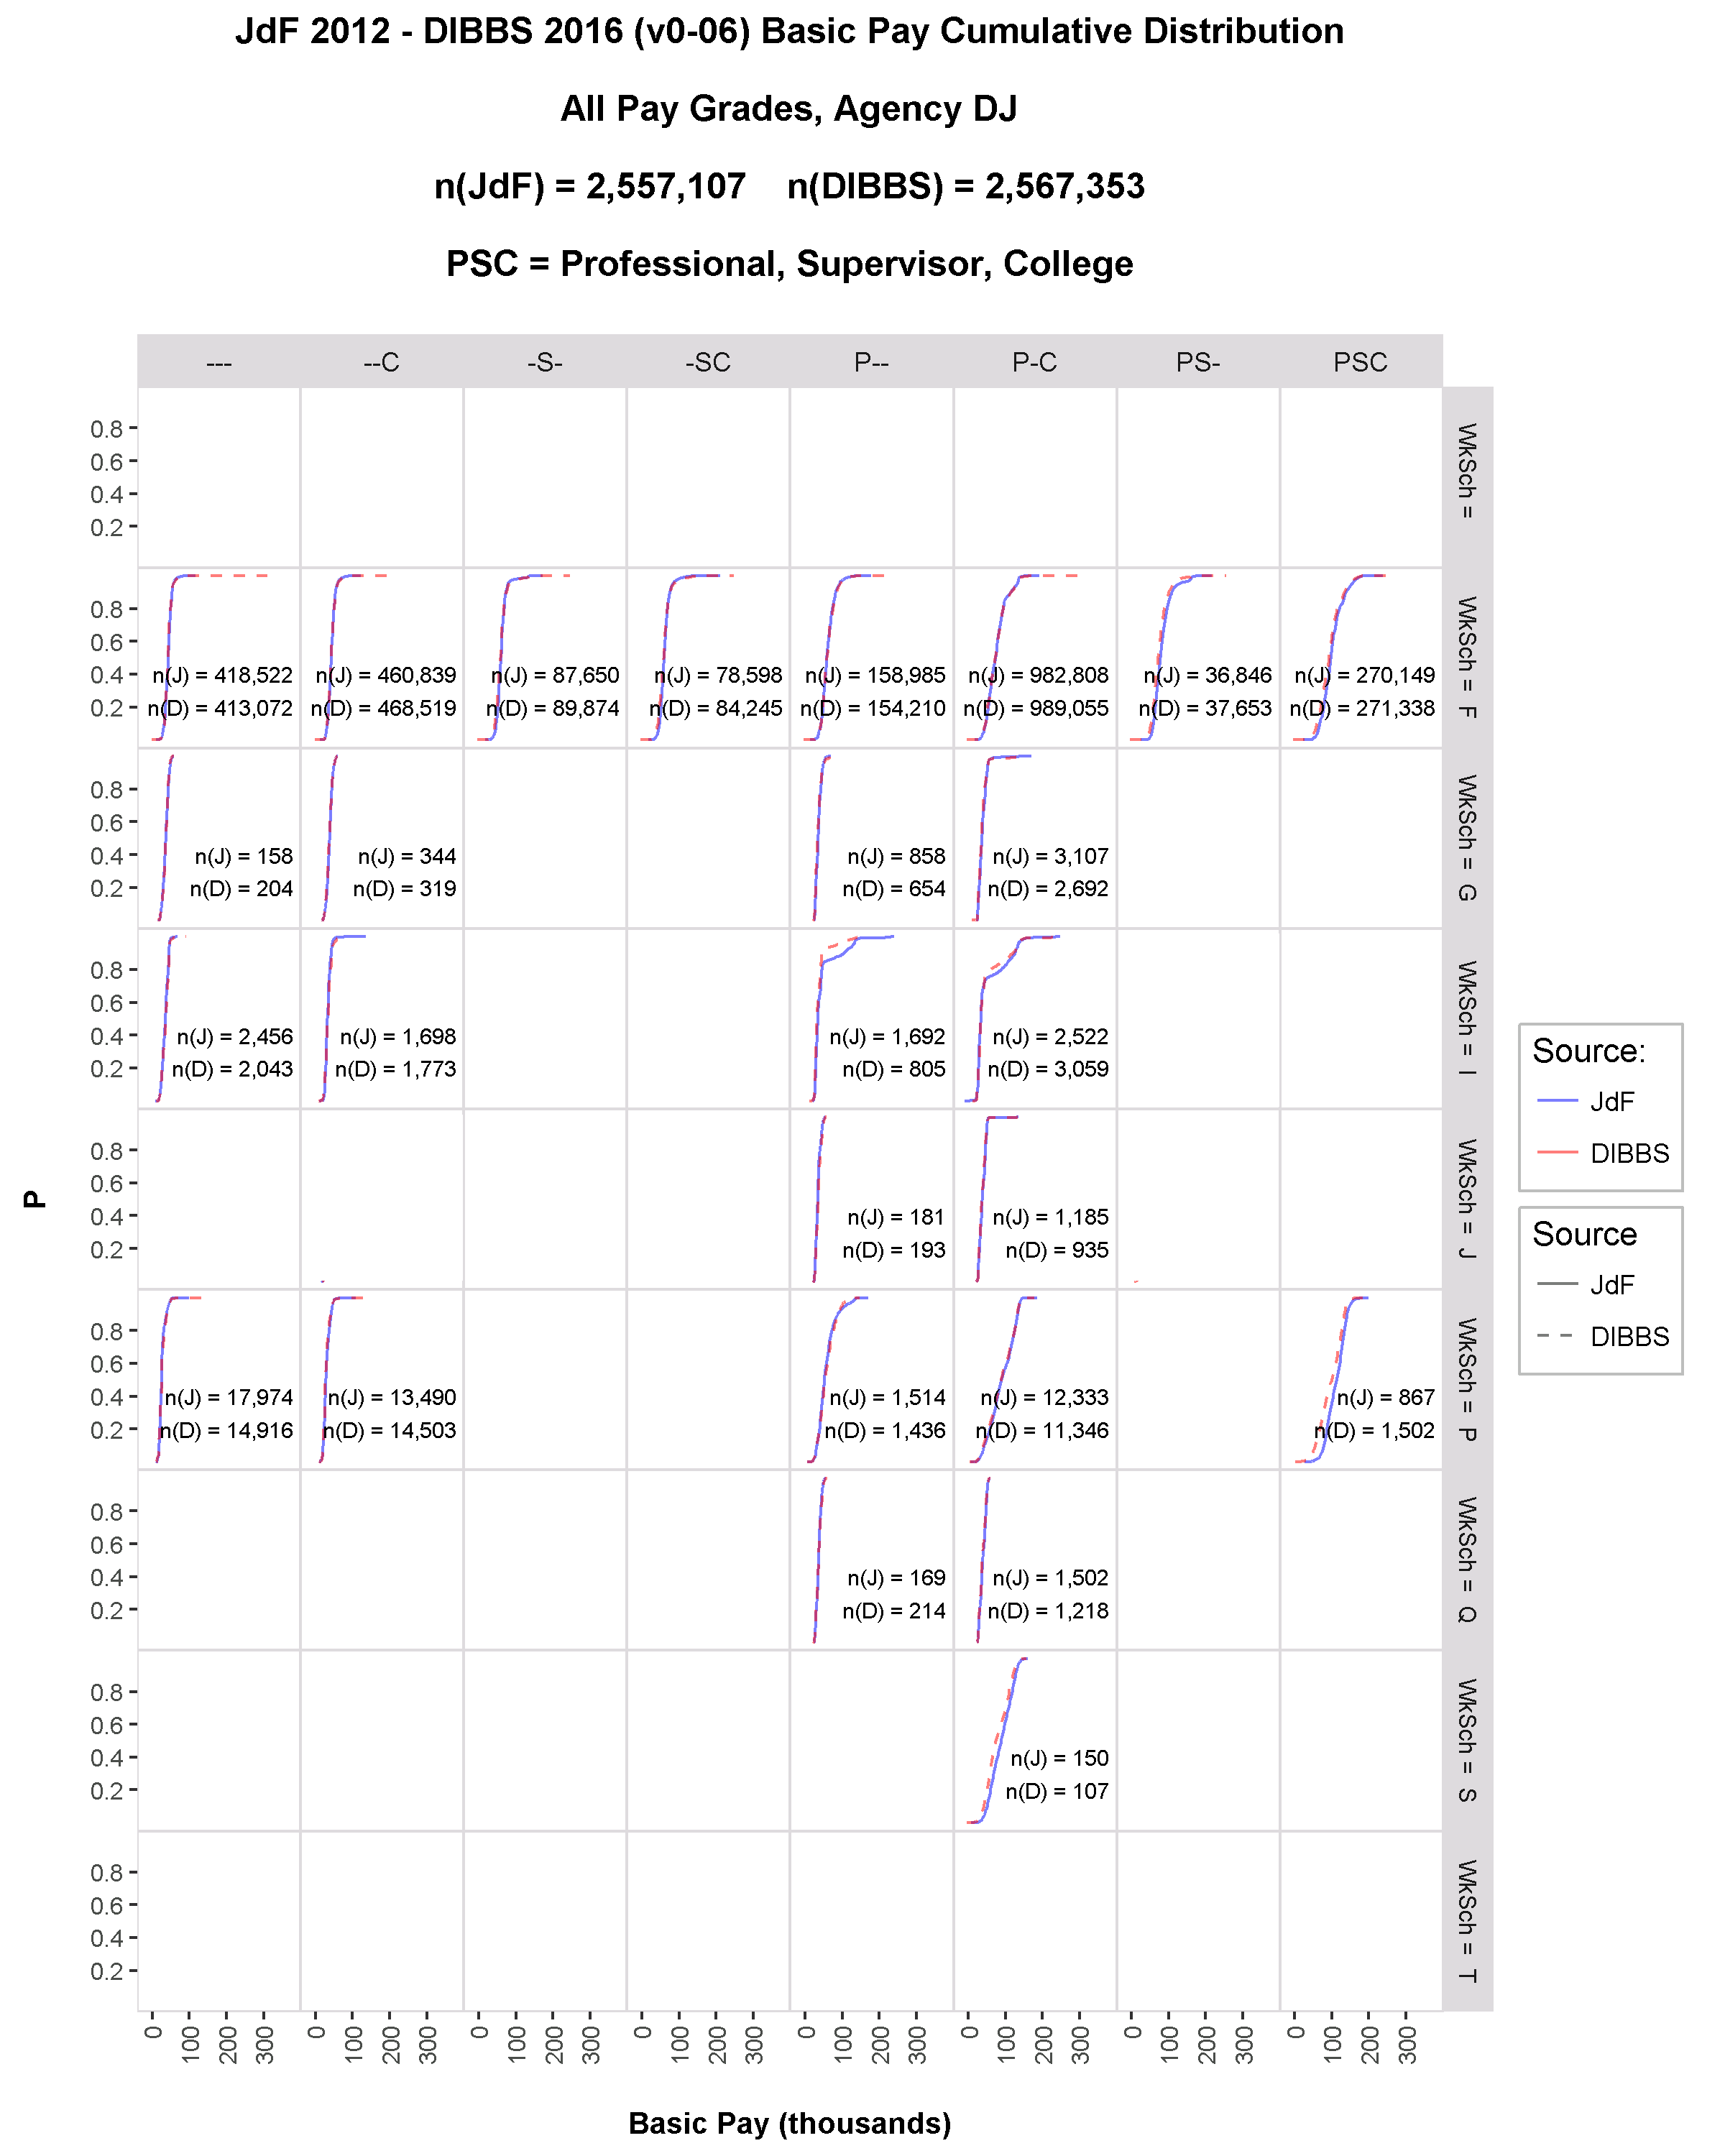
\includegraphics[width=6.5in, trim={0 0 1in 1.5in}, clip]{JdFDIBBSBasicPayCDFDJ.png}
    \caption{Basic pay distribution by joint professional, supervisory status, college education, and work schedule  categories.  Department of Justice (DJ).  Dashed line for synthetic data, solid line for authentic.}
    \label{figure:JdFDIBBSBasicPayCDFDJ}
\end{figure}

\clearpage

\begin{figure}[h]
    \centering
    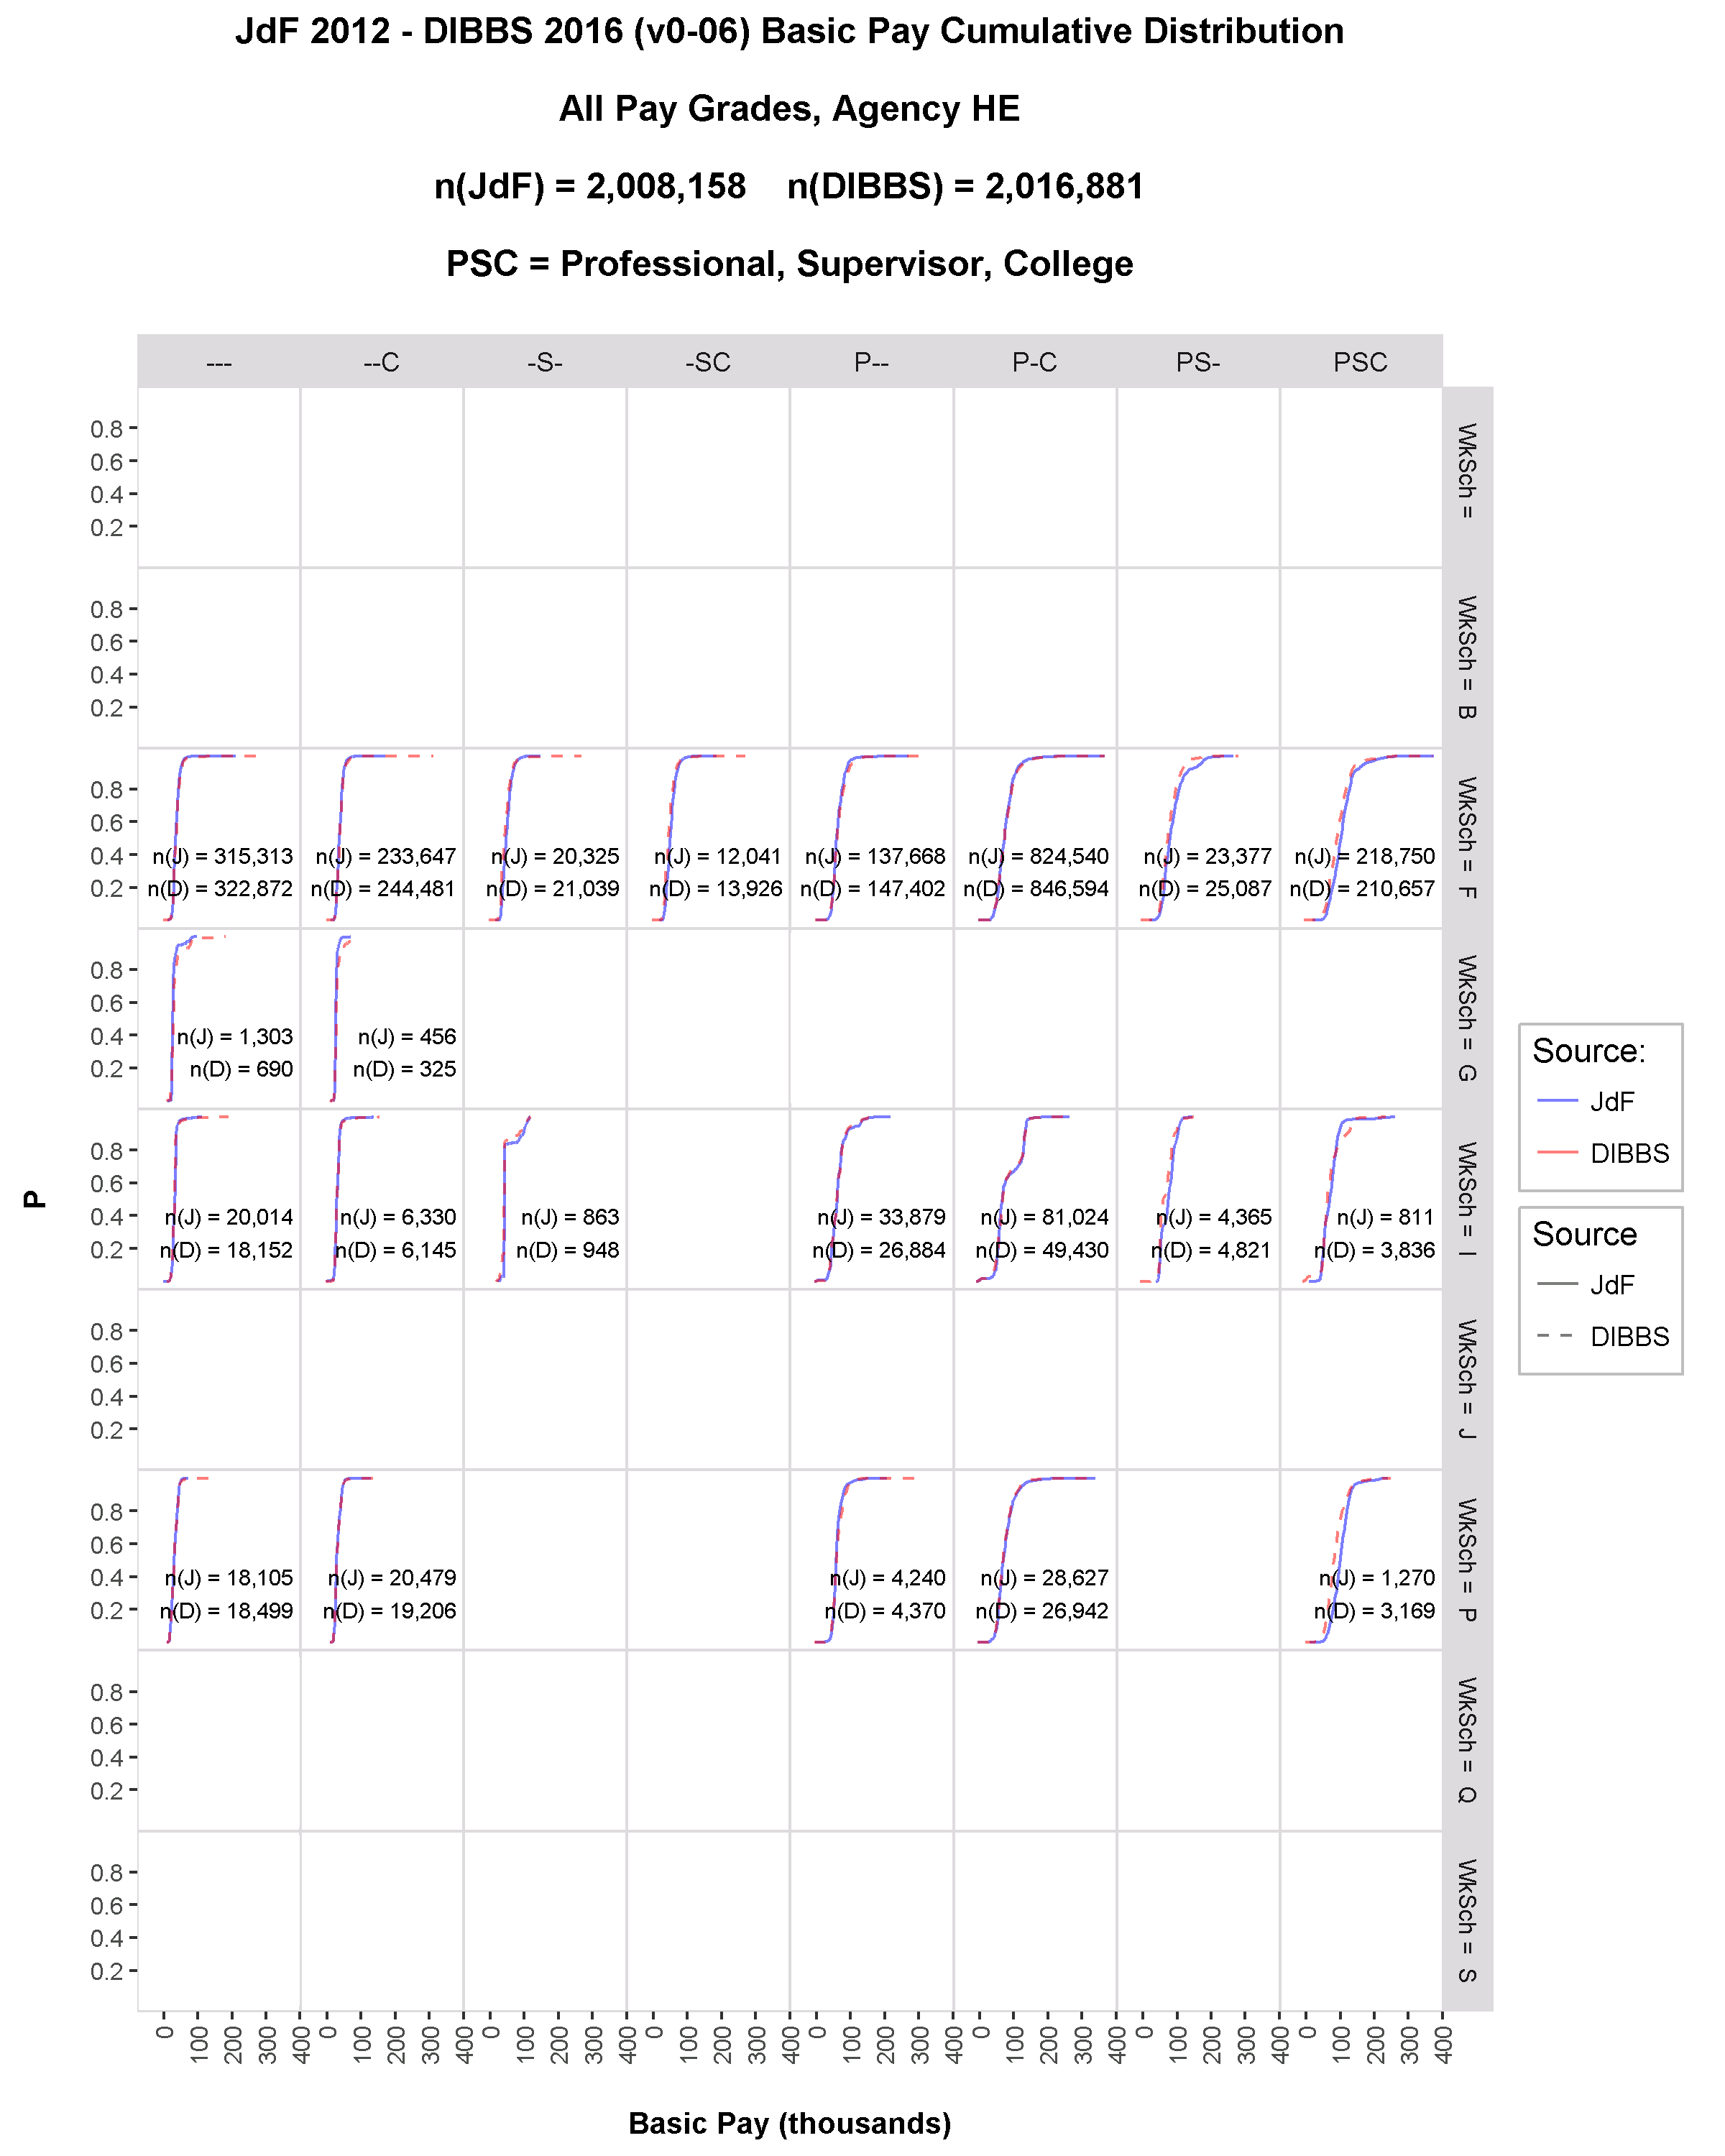
\includegraphics[width=6.5in, trim={0 0 1in 1.5in}, clip]{JdFDIBBSBasicPayCDFHE.png}
    \caption{Basic pay distribution by joint professional, supervisory status, college education, and work schedule  categories.  Department of Health and Human Services (HE).  Dashed line for synthetic data, solid line for authentic.}
    \label{figure:JdFDIBBSBasicPayCDFHE}
\end{figure}

\clearpage

\begin{figure}[h]
    \centering
    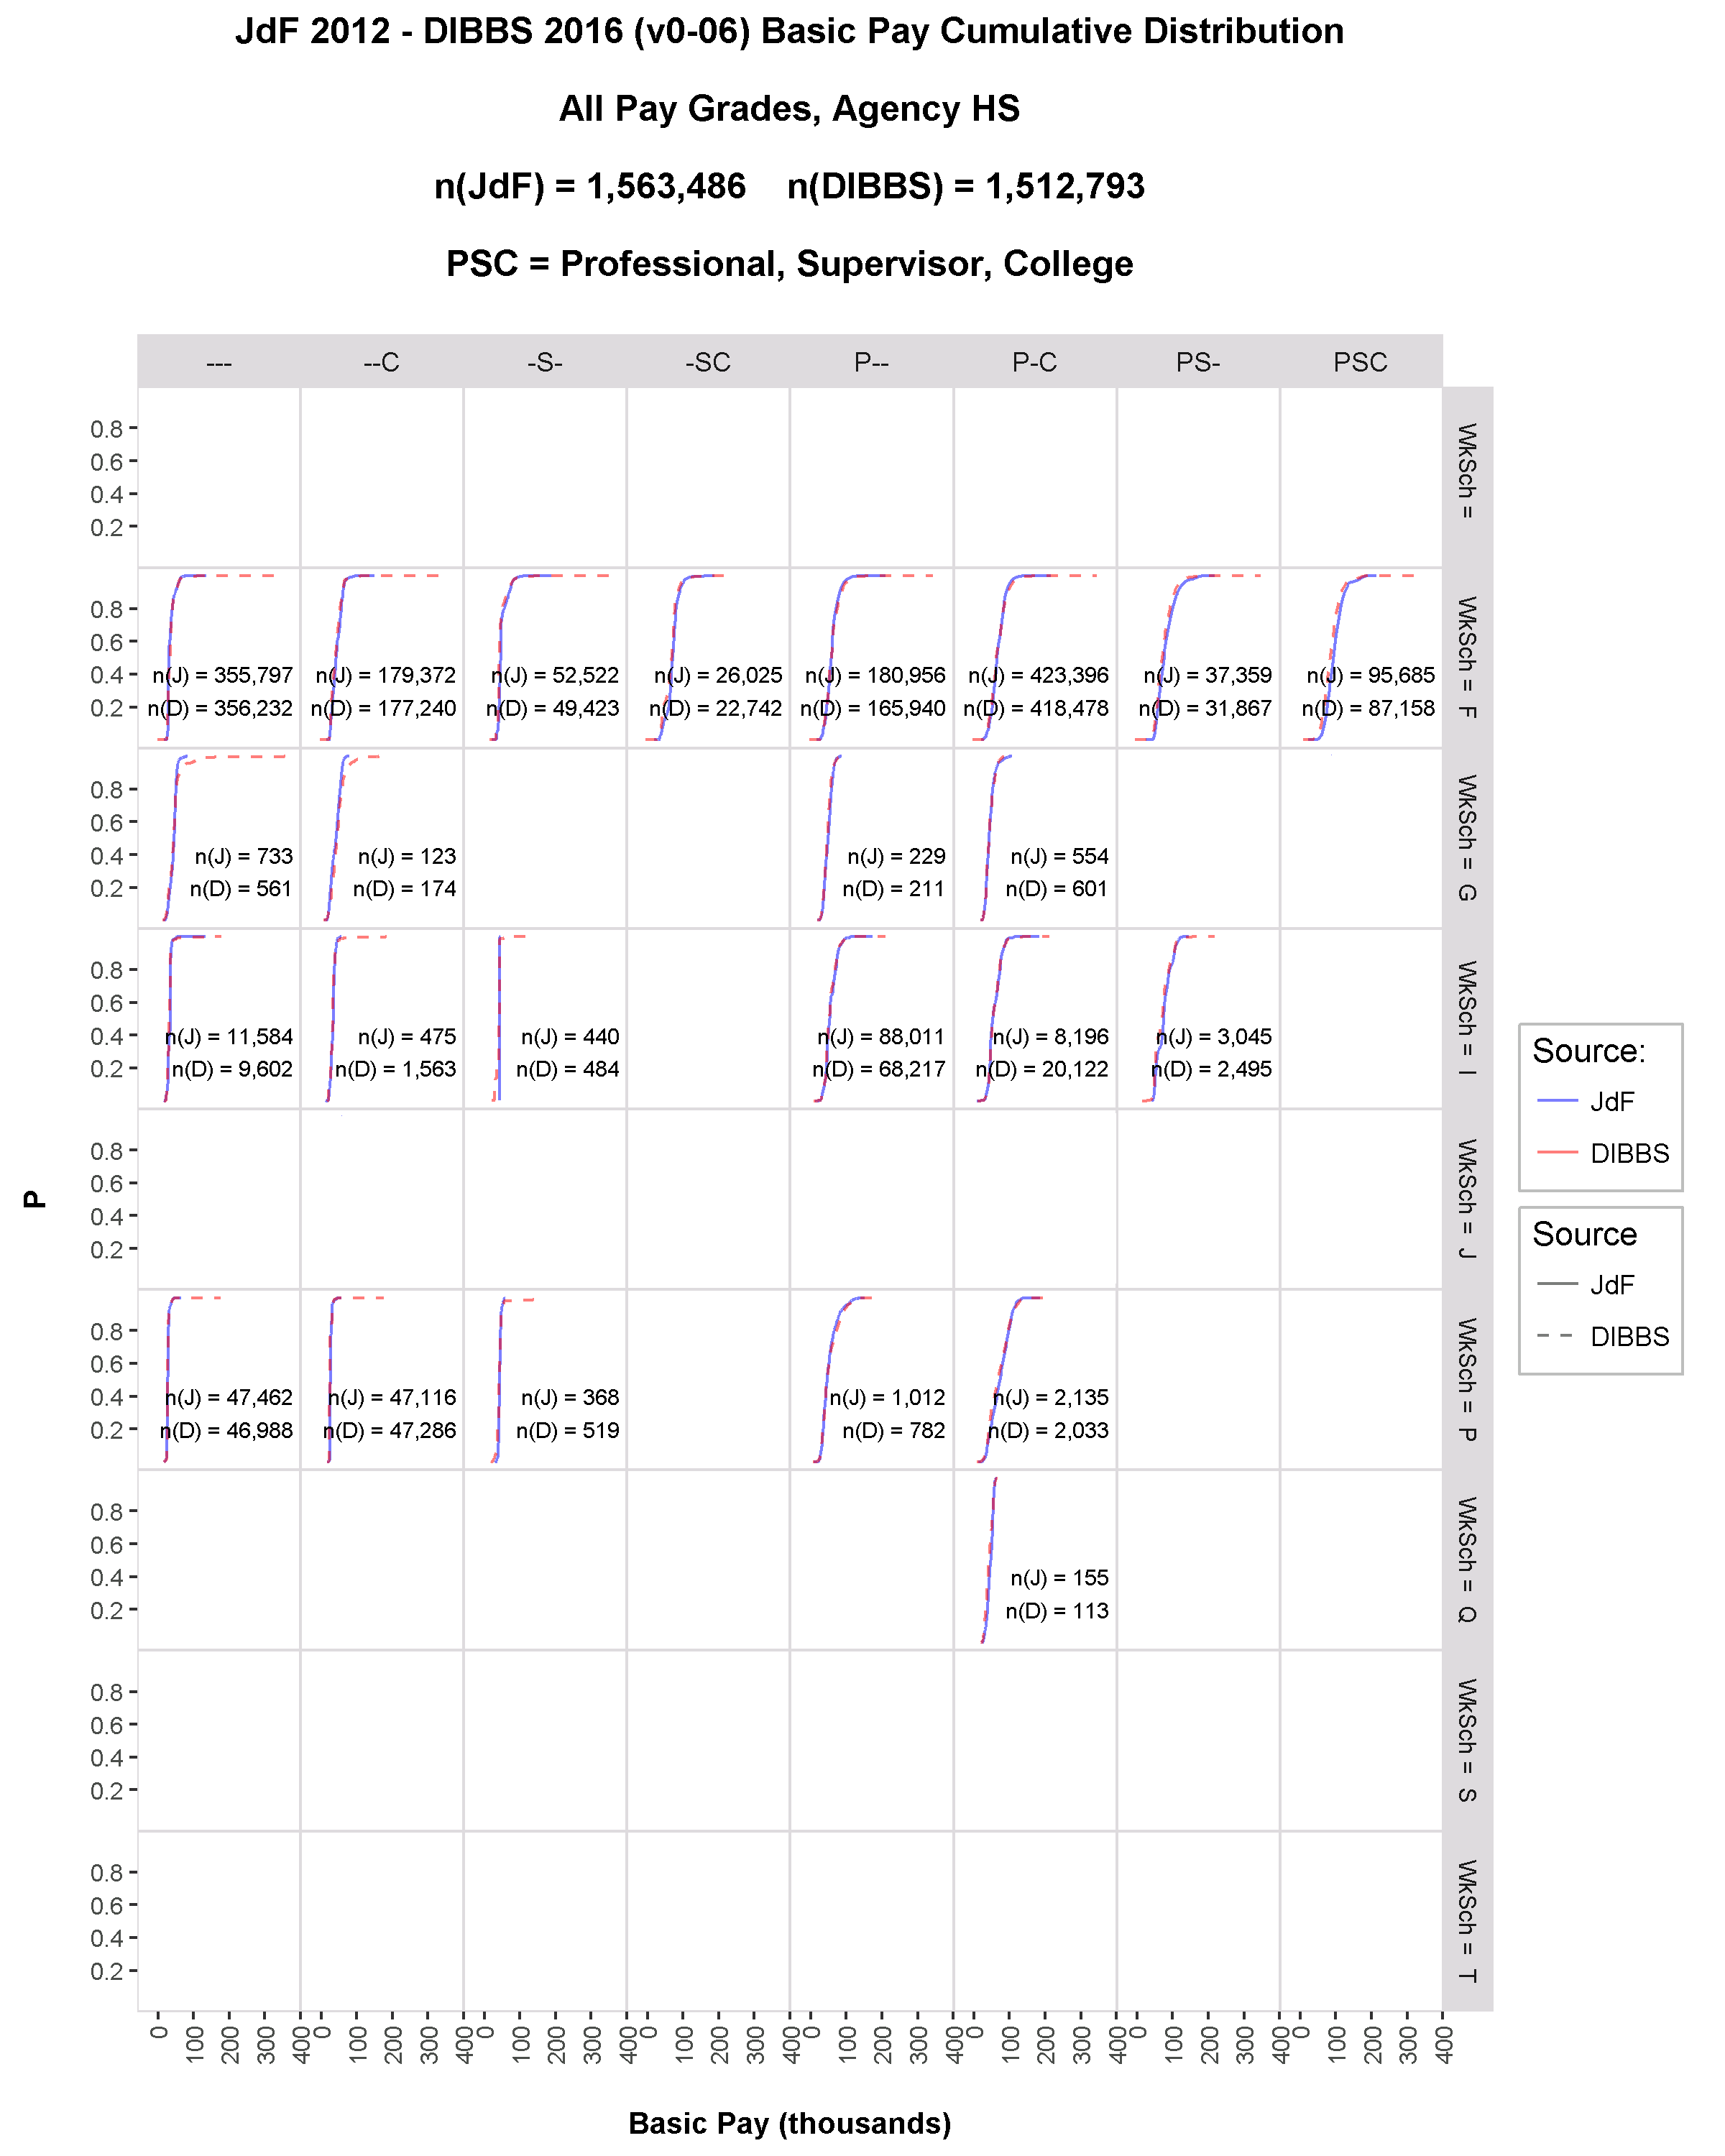
\includegraphics[width=6.5in, trim={0 0 1in 1.5in}, clip]{JdFDIBBSBasicPayCDFHS.png}
    \caption{Basic pay distribution by joint professional, supervisory status, college education, and work schedule  categories.  Department of Homeland Security (HS).  Dashed line for synthetic data, solid line for authentic.}
    \label{figure:JdFDIBBSBasicPayCDFHS}
\end{figure}

\clearpage

\begin{figure}[h]
    \centering
    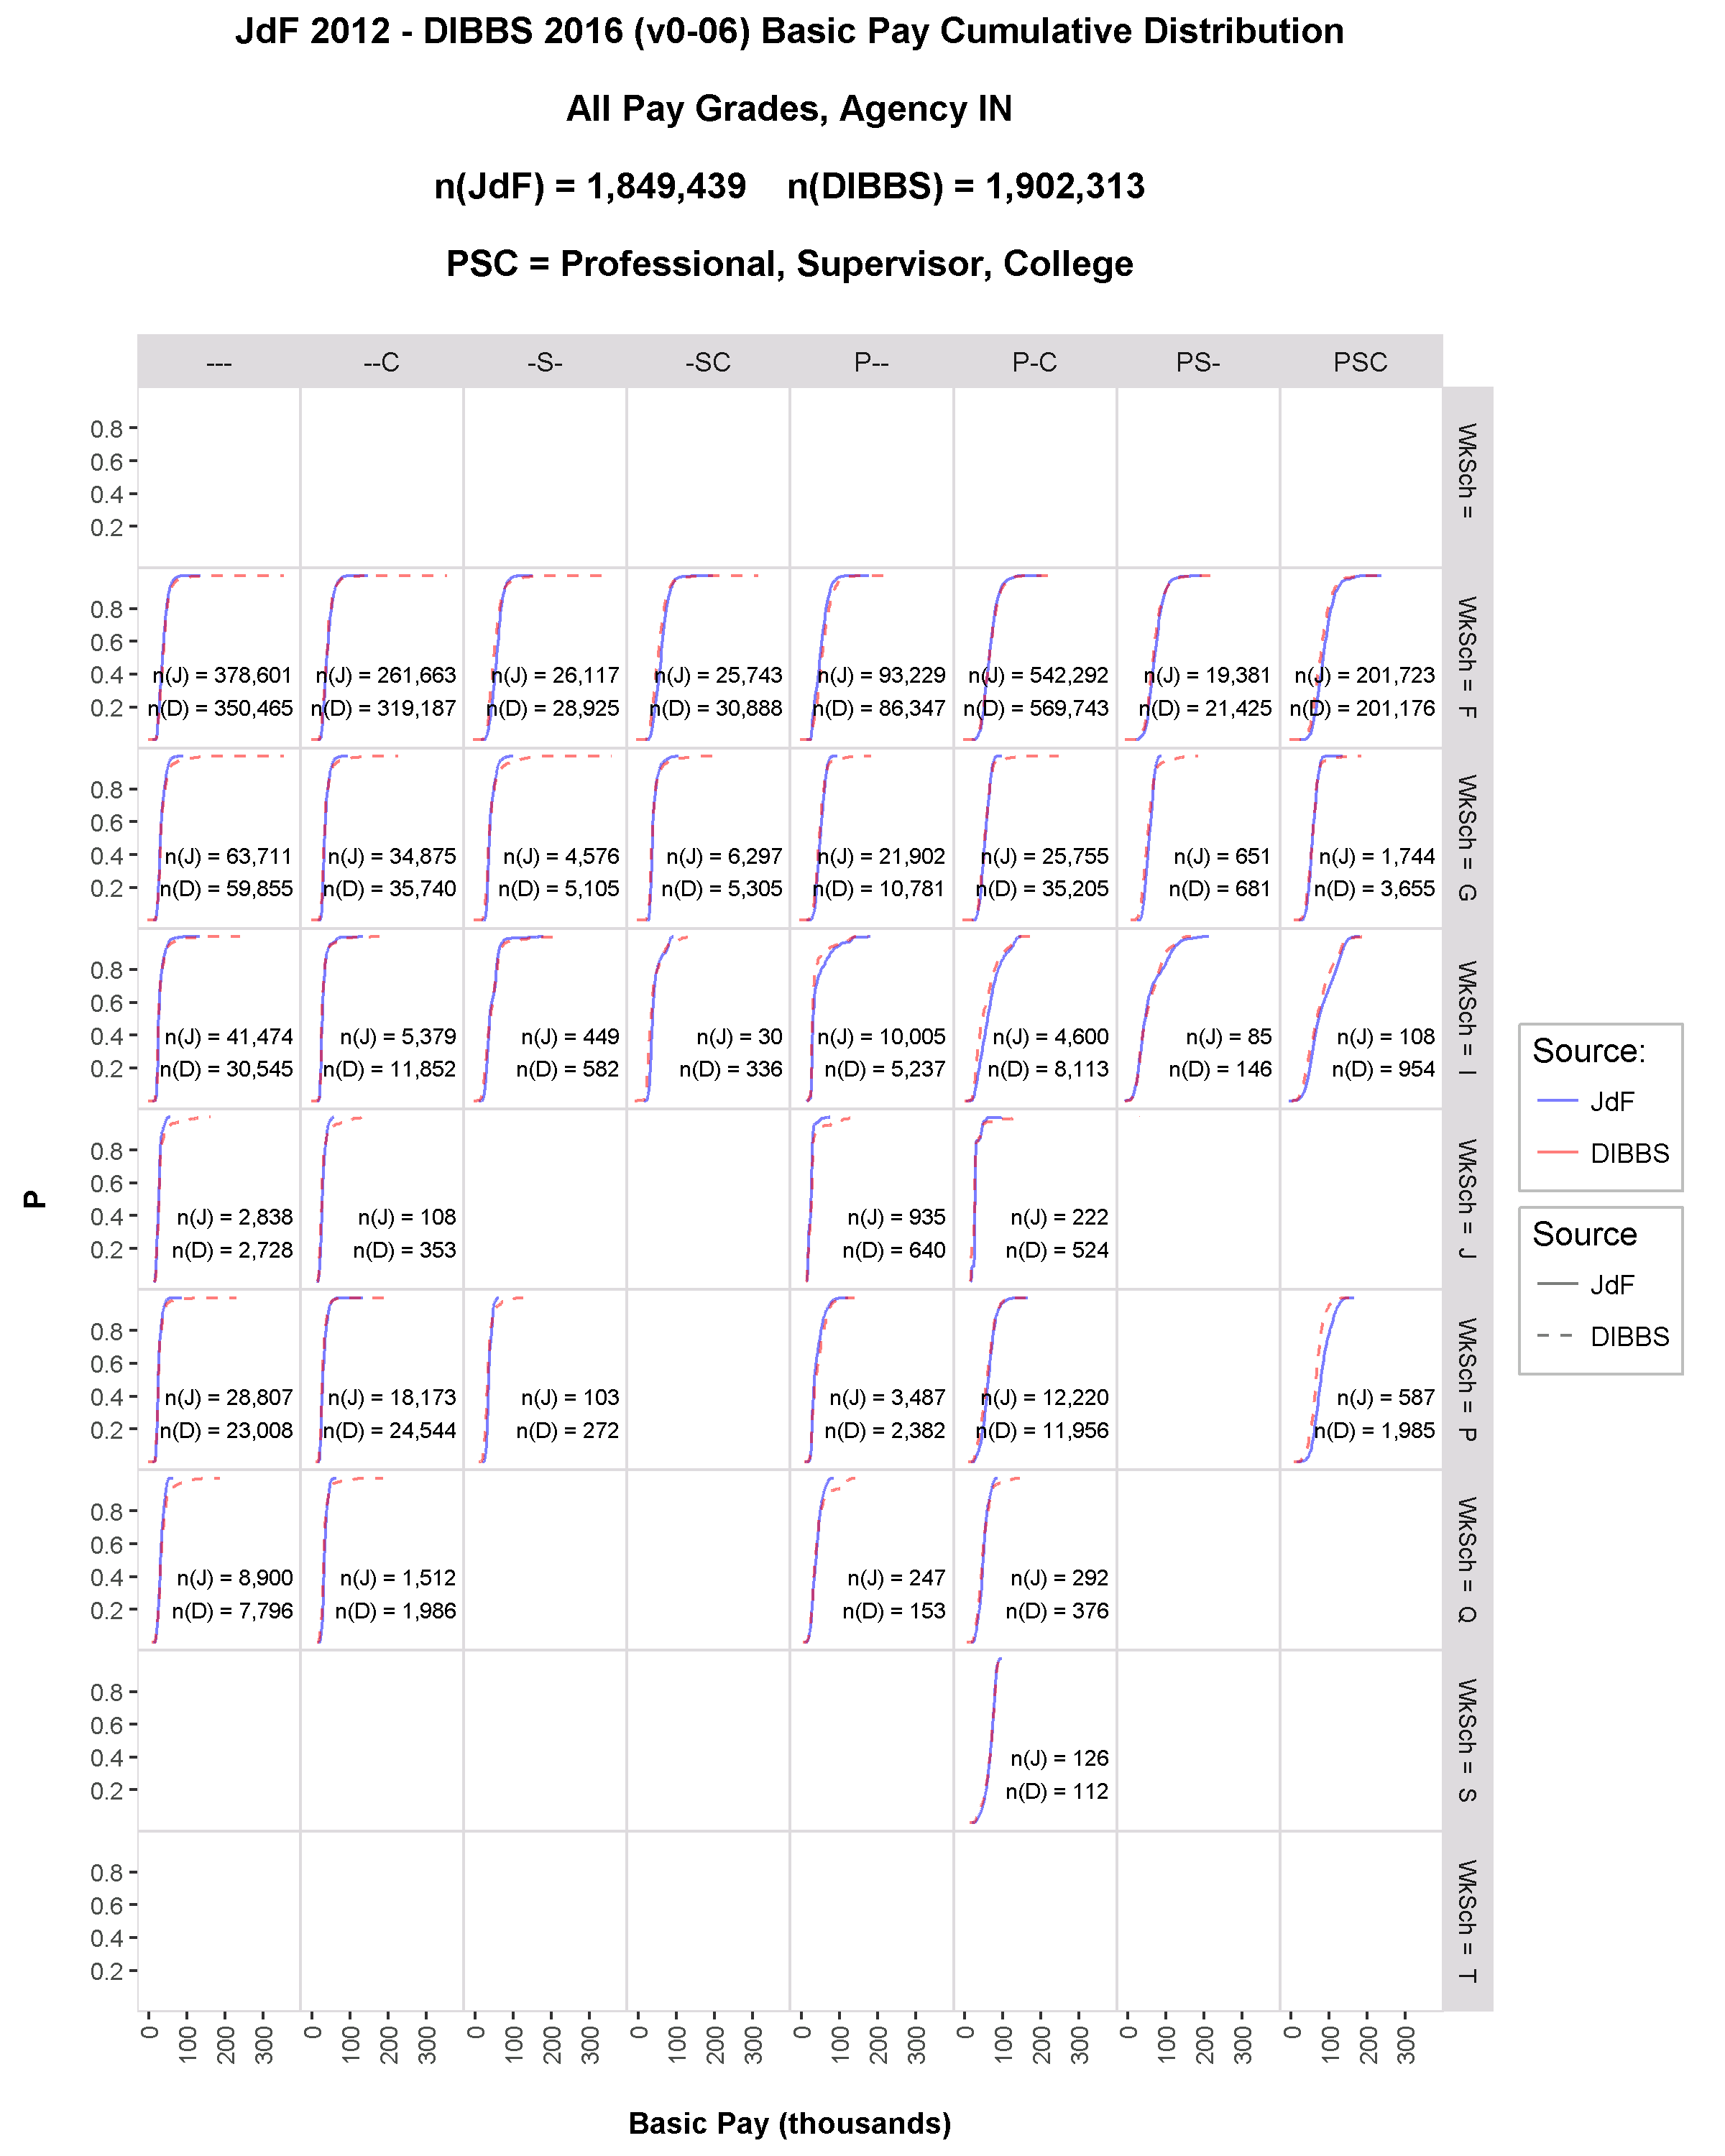
\includegraphics[width=6.5in, trim={0 0 1in 1.5in}, clip]{JdFDIBBSBasicPayCDFIN.png}
    \caption{Basic pay distribution by joint professional, supervisory status, college education, and work schedule  categories.  Department of Interior (IN).  Dashed line for synthetic data, solid line for authentic.}
    \label{figure:JdFDIBBSBasicPayCDFIN}
\end{figure}

\clearpage

\begin{figure}[h]
    \centering
    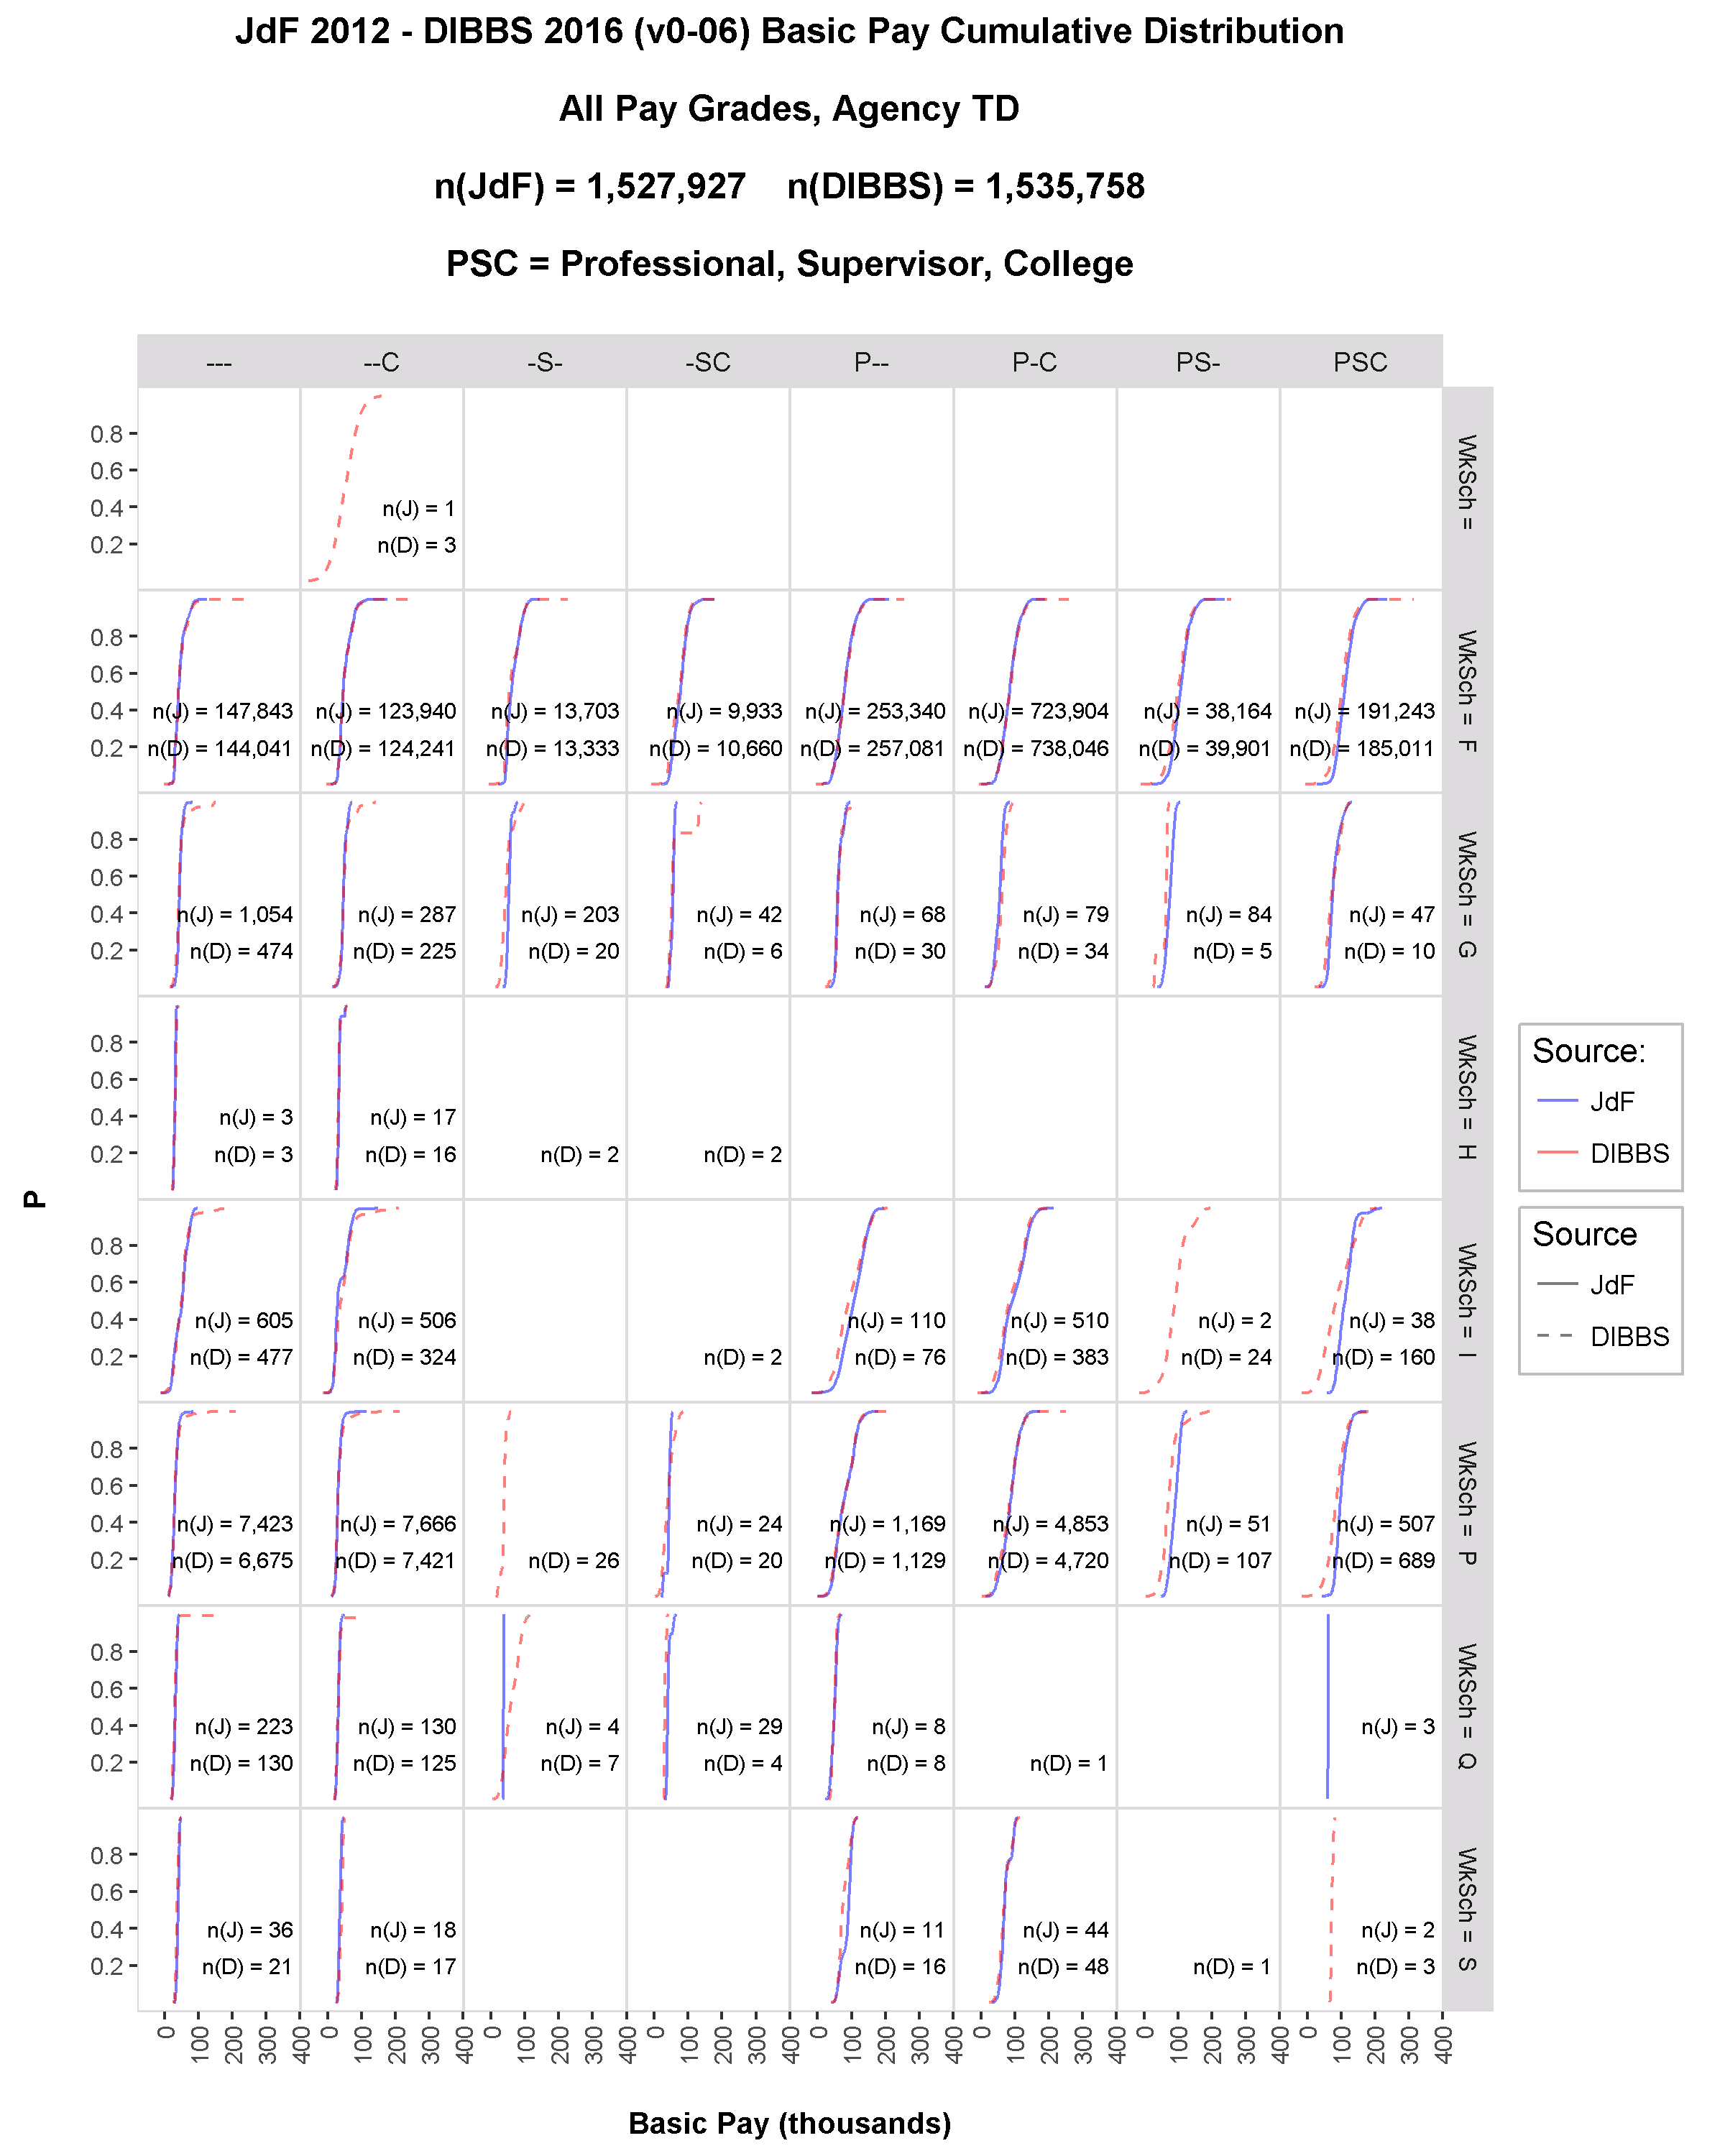
\includegraphics[width=6.5in, trim={0 0 1in 1.5in}, clip]{JdFDIBBSBasicPayCDFTD.png}
    \caption{Basic pay distribution by joint professional, supervisory status, college education, and work schedule  categories.  Department of Transportation (TD).  Dashed line for synthetic data, solid line for authentic.}
    \label{figure:JdFDIBBSBasicPayCDFTD}
\end{figure}

\clearpage

\begin{figure}[h]
    \centering
    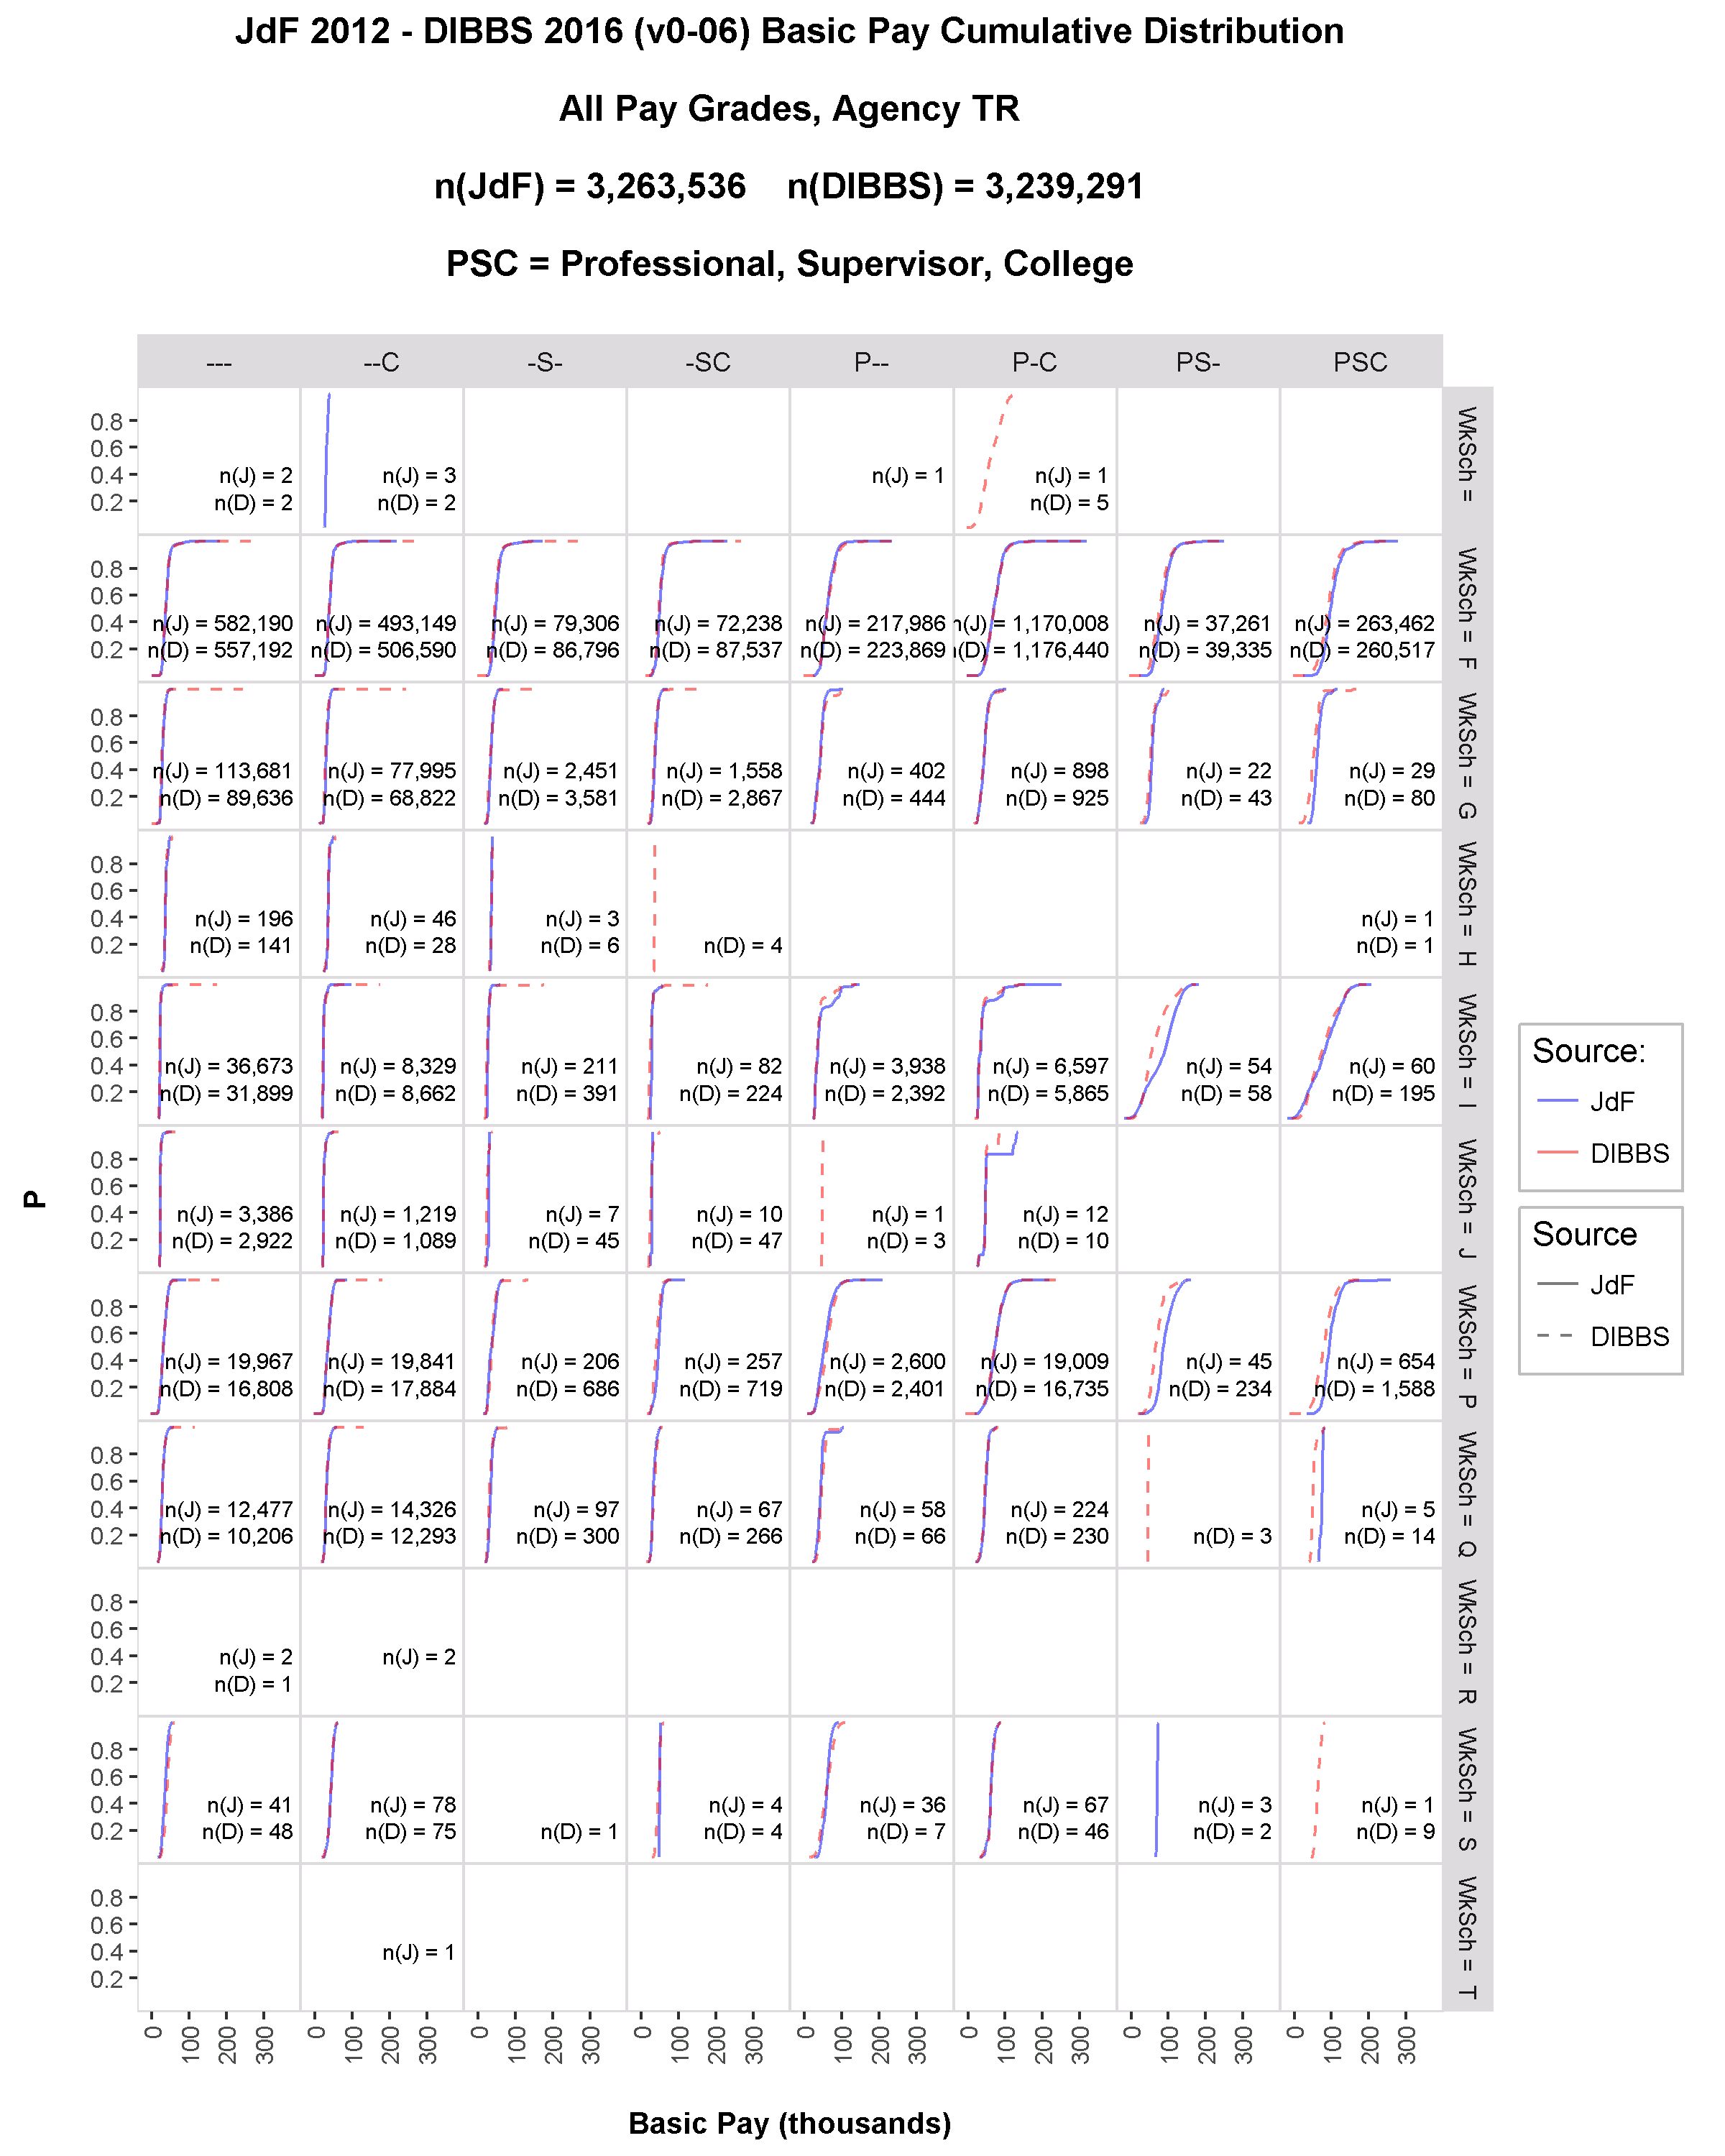
\includegraphics[width=6.5in, trim={0 0 1in 1.5in}, clip]{JdFDIBBSBasicPayCDFTR.png}
    \caption{Basic pay distribution by joint professional, supervisory status, college education, and work schedule  categories.  Department of Treasury (TR).  Dashed line for synthetic data, solid line for authentic.}
    \label{figure:JdFDIBBSBasicPayCDFTR}
\end{figure}

\clearpage

\begin{figure}[h]
    \centering
    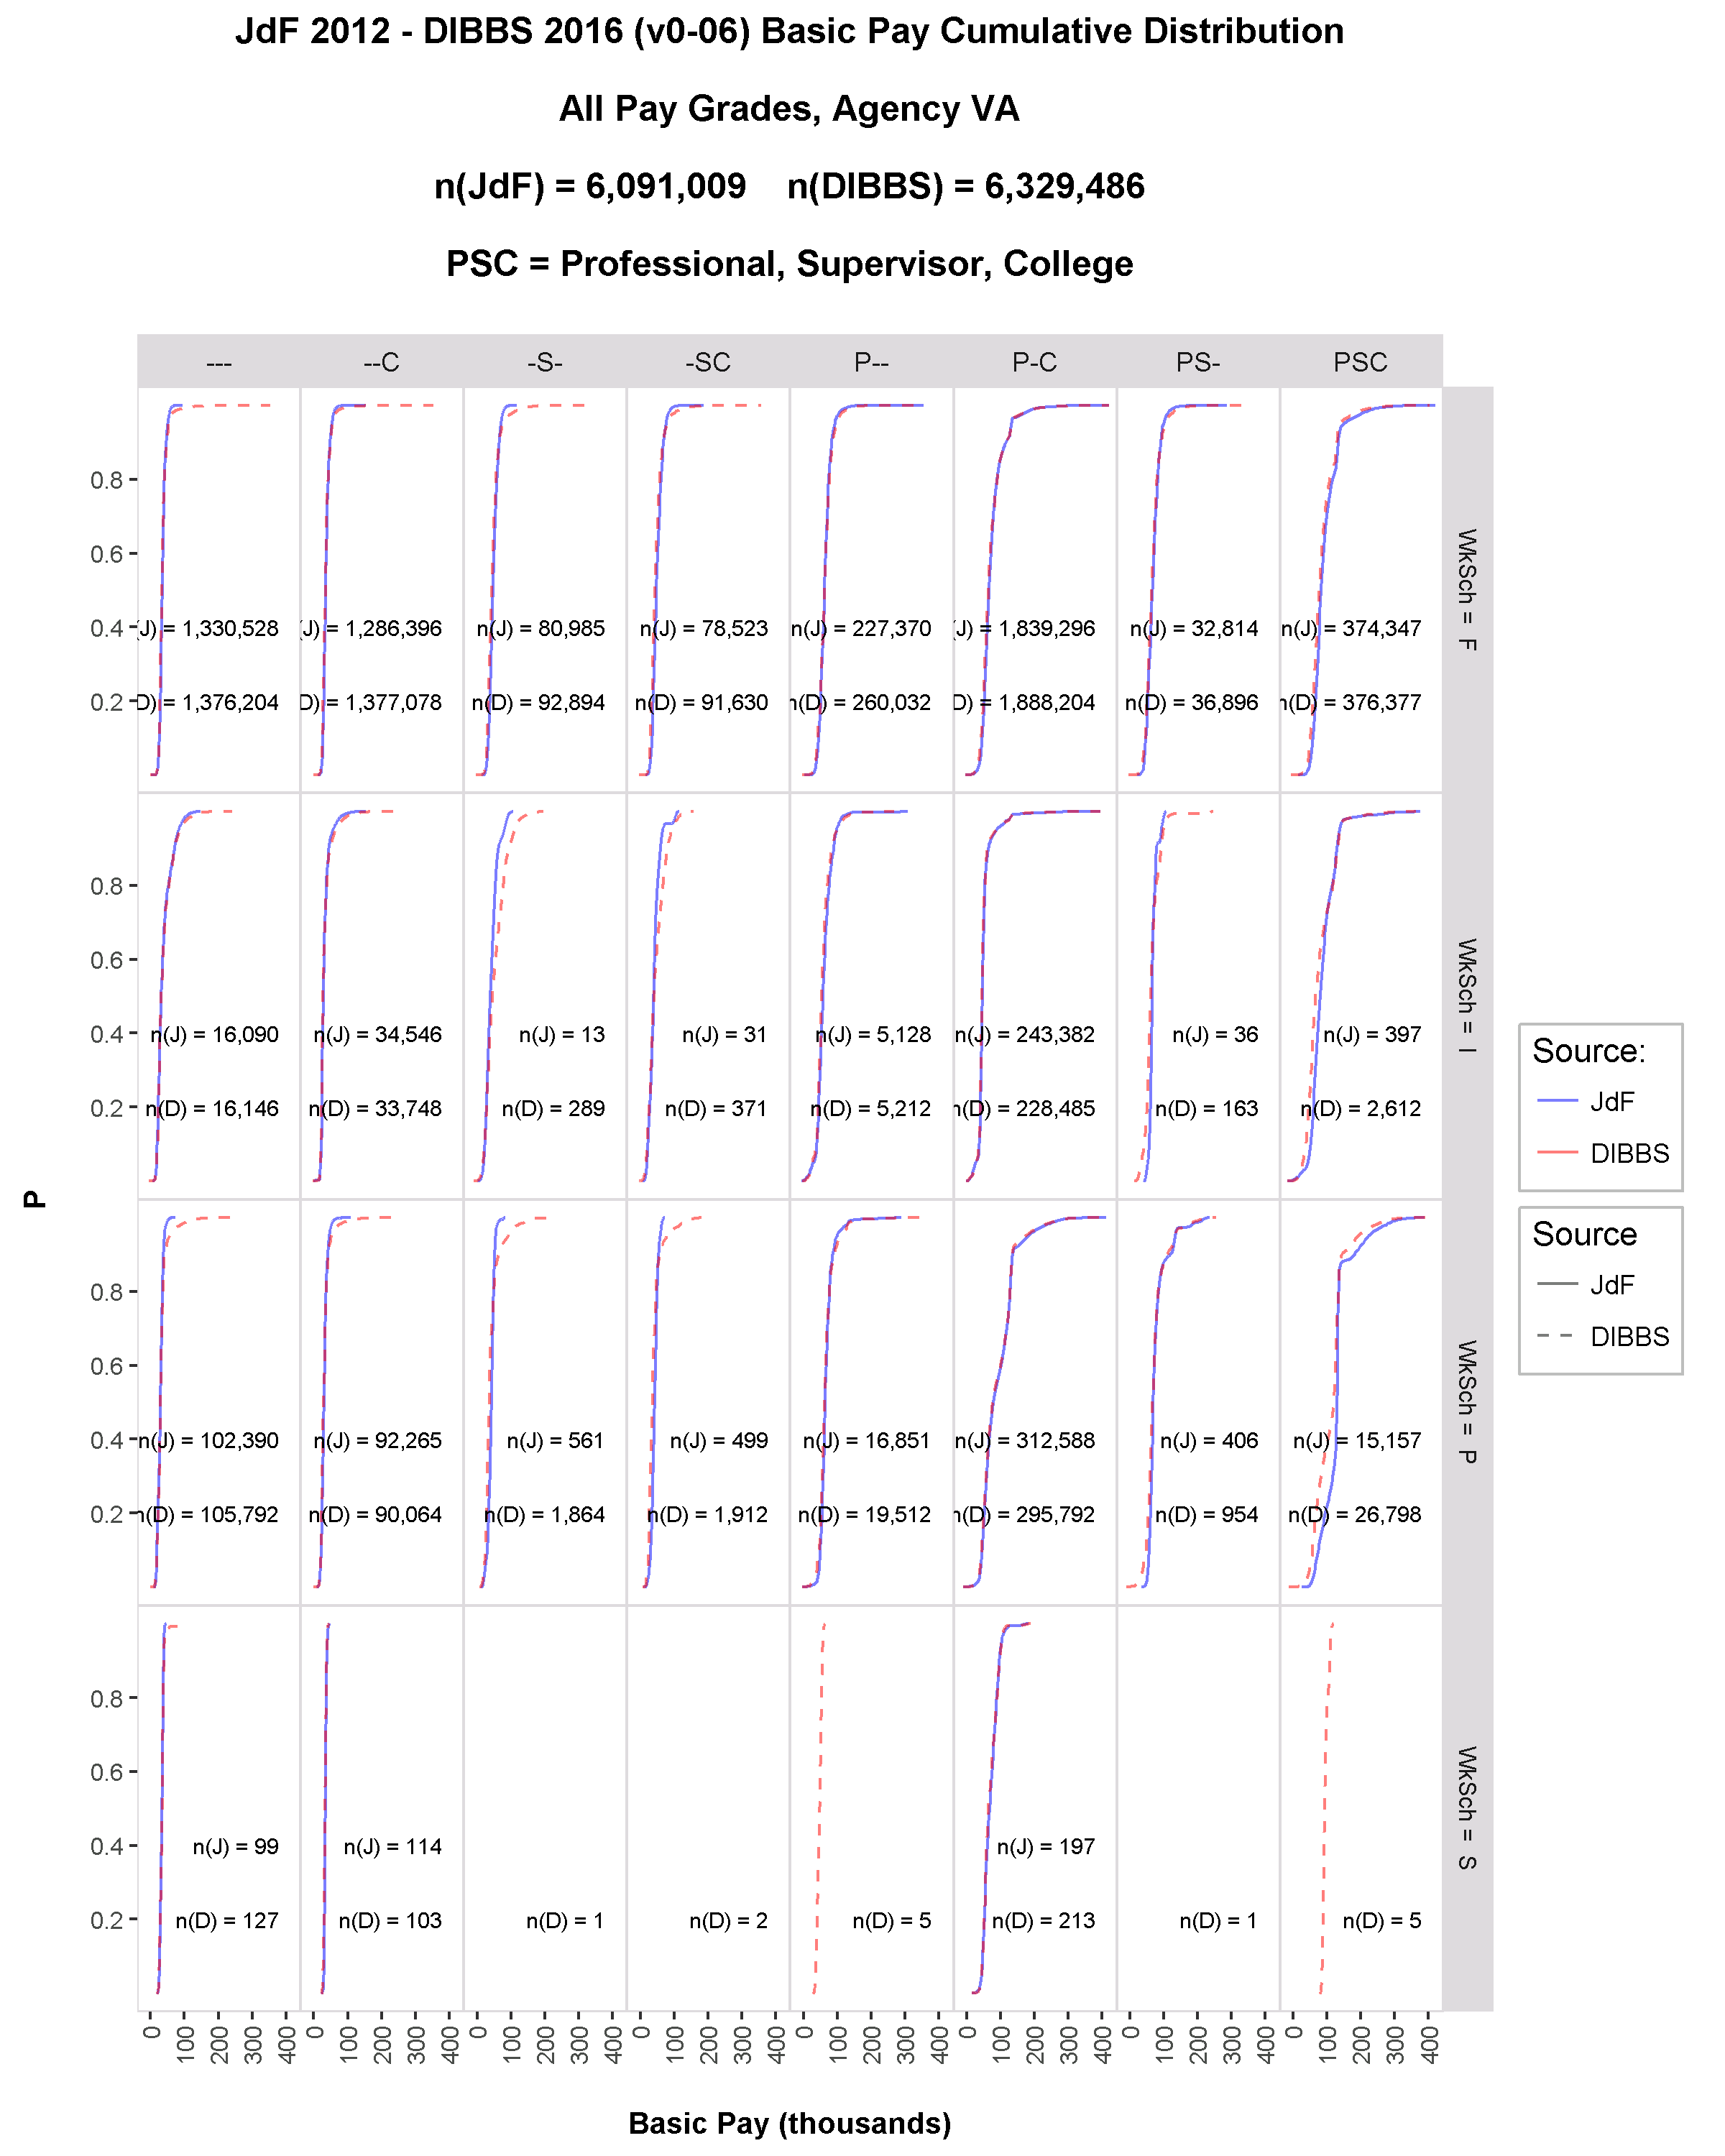
\includegraphics[width=6.5in, trim={0 0 1in 1.5in}, clip]{JdFDIBBSBasicPayCDFVA.png}
    \caption{Basic pay distribution by joint professional, supervisory status, college education, and work schedule  categories.  Department of Veterans Affairs (VA).  Dashed line for synthetic data, solid line for authentic.}
    \label{figure:JdFDIBBSBasicPayCDFVA}
\end{figure}

\clearpage

DISTRIBUTION OF BASIC PAY BY OCCUPATION AND SUPERVISORY STATUS\\

803 distinct occupations are represented in the data supplied by OPM.  To verify distribution of basic pay by occupation and supervisory status in the synthetic data, box plots consisting of a pair of authentic/synthetic distributions for each occupation were constructed.  Figures \ref{figure:JdFDIBBSBasicPaySupervisoryStatusOccupation1} through \ref{figure:JdFDIBBSBasicPaySupervisoryStatusOccupation3} show box plots for the first 120 occupations in order of occupation code.  Trade, or blue collar, occupations begin at code 2500.  Figures \ref{figure:JdFDIBBSBasicPaySupervisoryStatusOccupation4} and \ref{figure:JdFDIBBSBasicPaySupervisoryStatusOccupation5} show the distributions of the first 80 of these occupations.  Remaining occupations exhibit patterns similar to those presented.\\

Observations:  Median pay and inter-quartile ranges appear consistent between data sets.  Upper tails of distributions of in the synthetic data generally appear greater than corresponding authentic distributions, particulary for trade occupations.  Note that, of the 318 trade occupations represented in the authentic data, 190 have proportion female observations less than 0.05.  Given disparity in federal employee pay by gender \citep{BoltondeFigGenderPayGap2017} and a requirement, for protection of privacy, of a degree of modification of gender and occupation in synthetic observations, differences in pay extremes may be expected.\\

\begin{figure}[h]
    \centering
    \begin{subfigure}{1\textwidth}
        \centering
        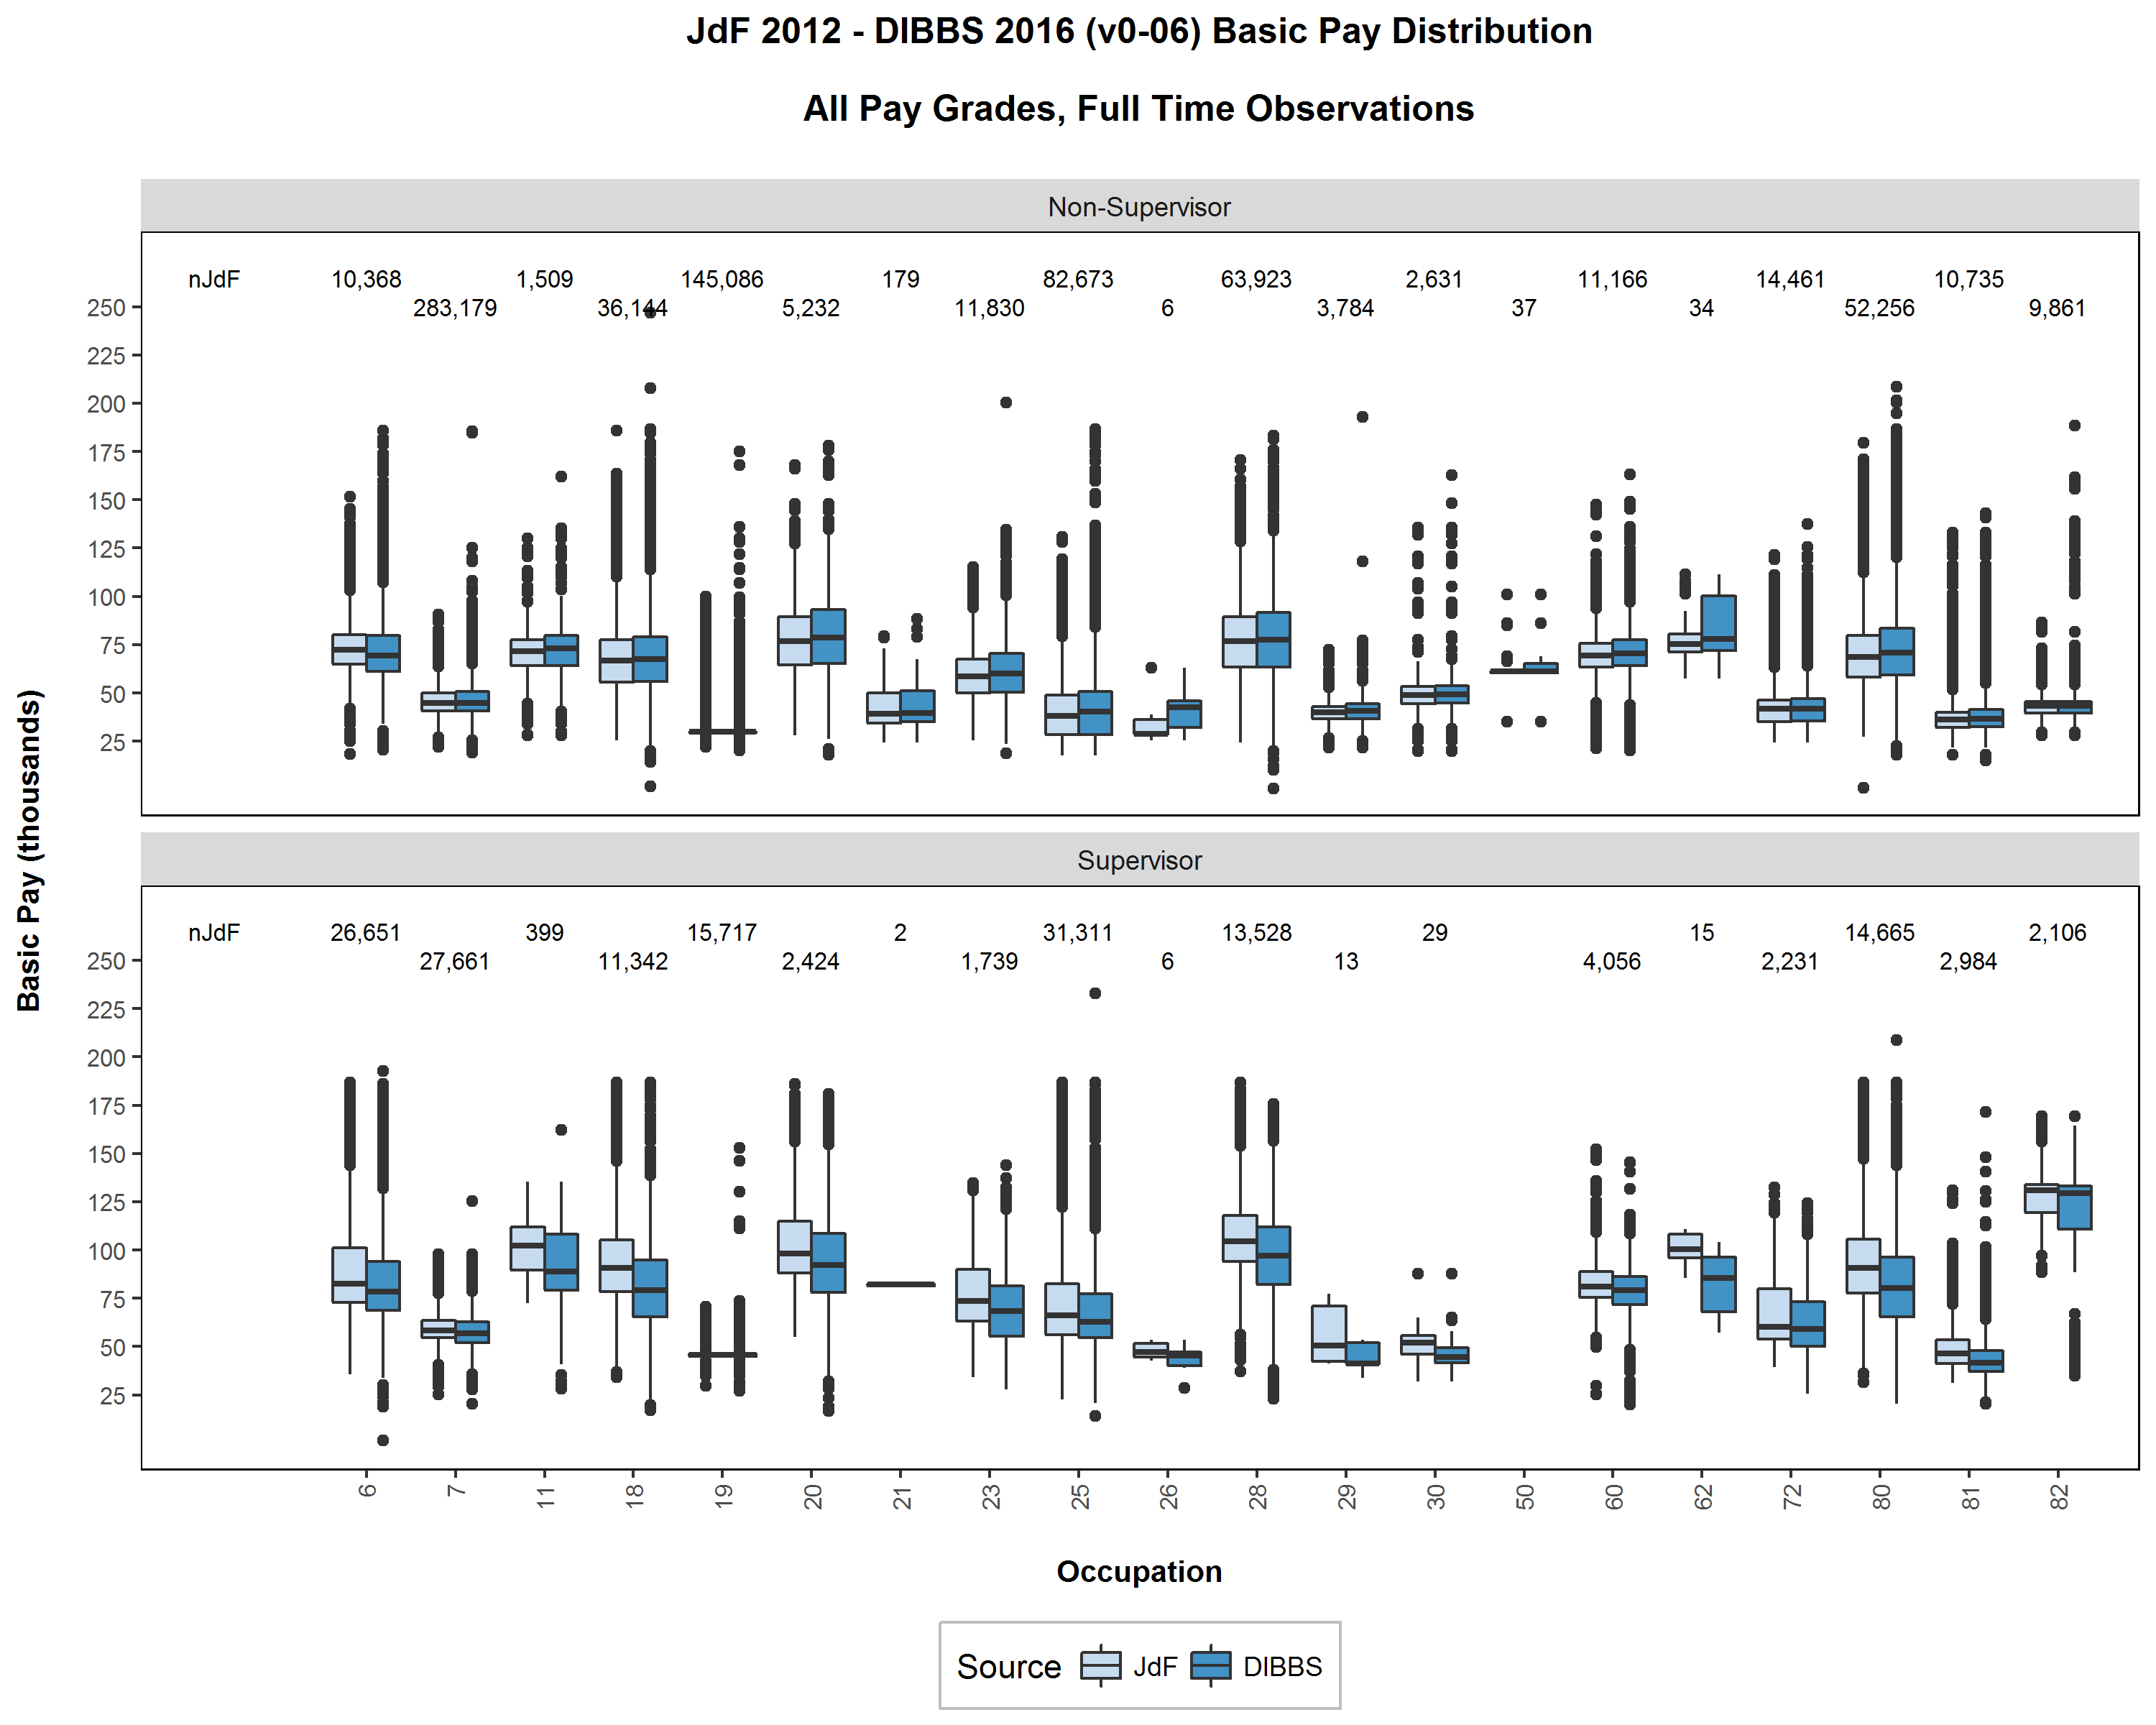
\includegraphics[width=6in, trim={0 1in 0 0.75in}, clip]{JdFDIBBSBasicPaySupervisoryStatusOccupation1.png}
        \caption{Occupations 0006 through 0082}
        \vspace{10pt}
    \end{subfigure}
    \begin{subfigure}{1\textwidth}
        \centering
        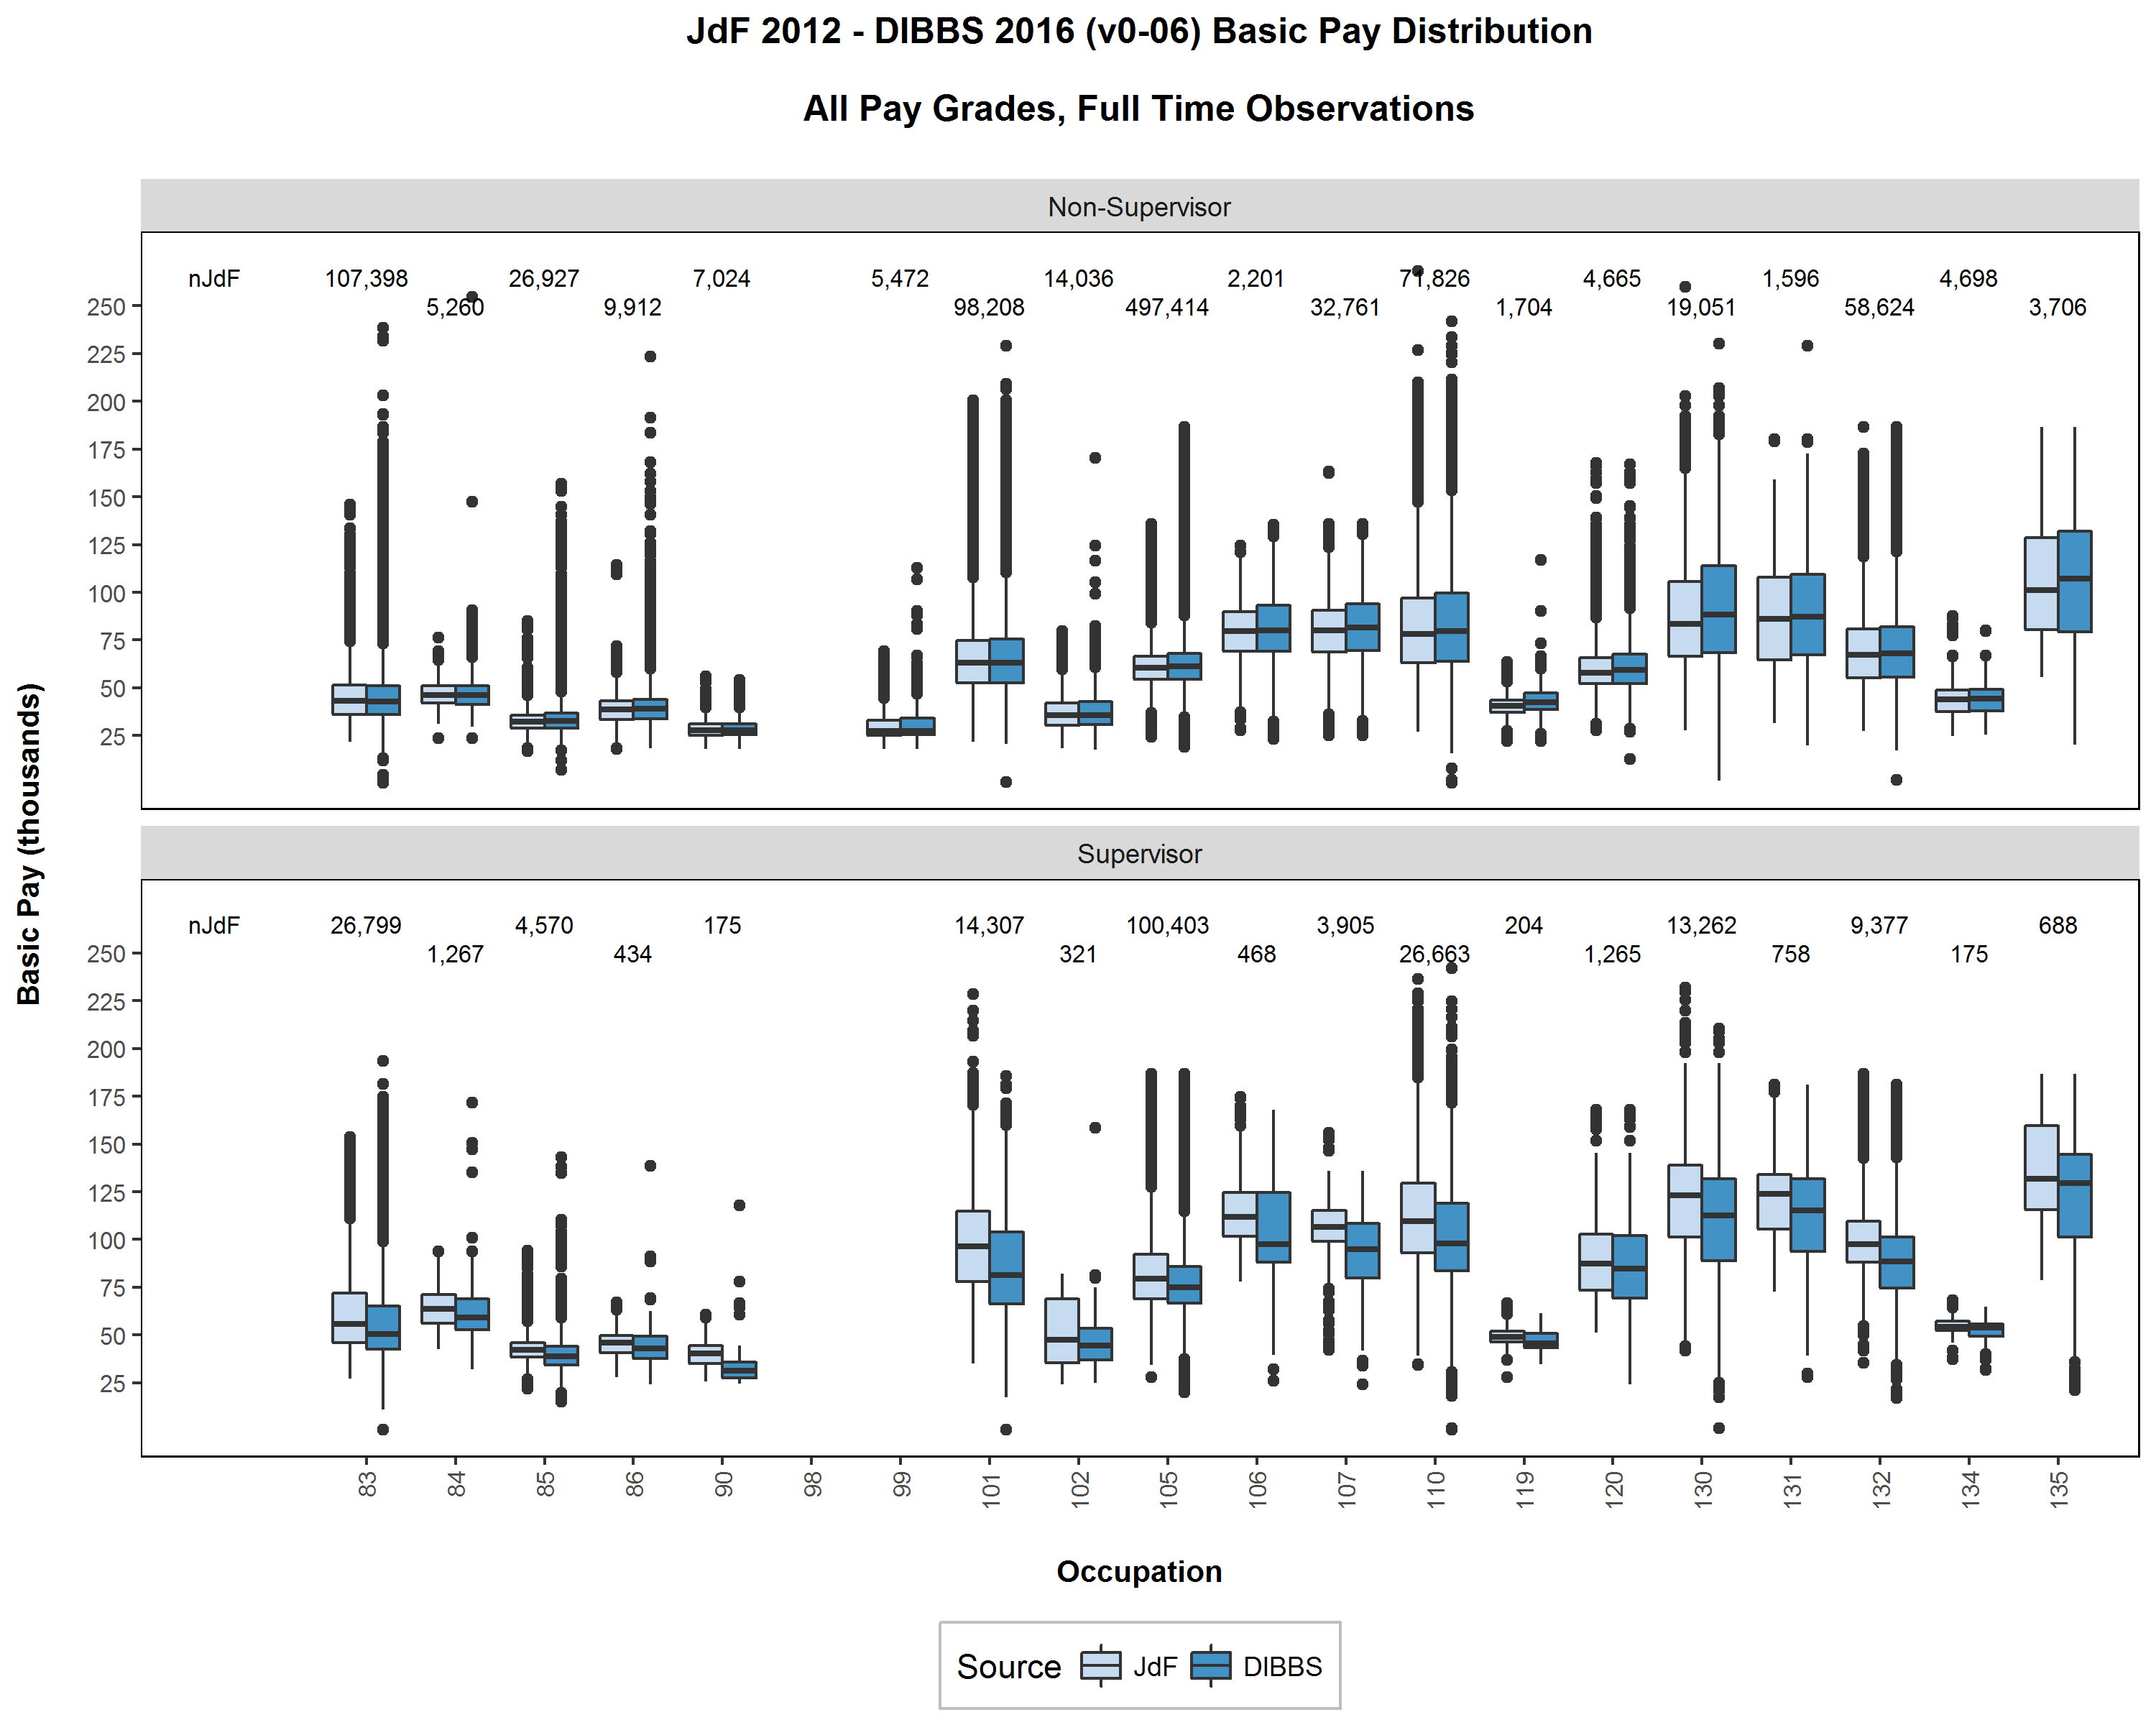
\includegraphics[width=6in, trim={0 1in 0 0.75in}, clip]{JdFDIBBSBasicPaySupervisoryStatusOccupation21.png}
        \caption{Occupations 0083 through 0135}
        \vspace{10pt}
    \end{subfigure}
    \caption{Basic pay distribution by occupation and supervisor status.  All agencies combined.  Authentic boxes on left, synthetic on right.}
    \label{figure:JdFDIBBSBasicPaySupervisoryStatusOccupation1}
\end{figure}

\clearpage

\begin{figure}[h]
    \centering
    \begin{subfigure}{1\textwidth}
        \centering
        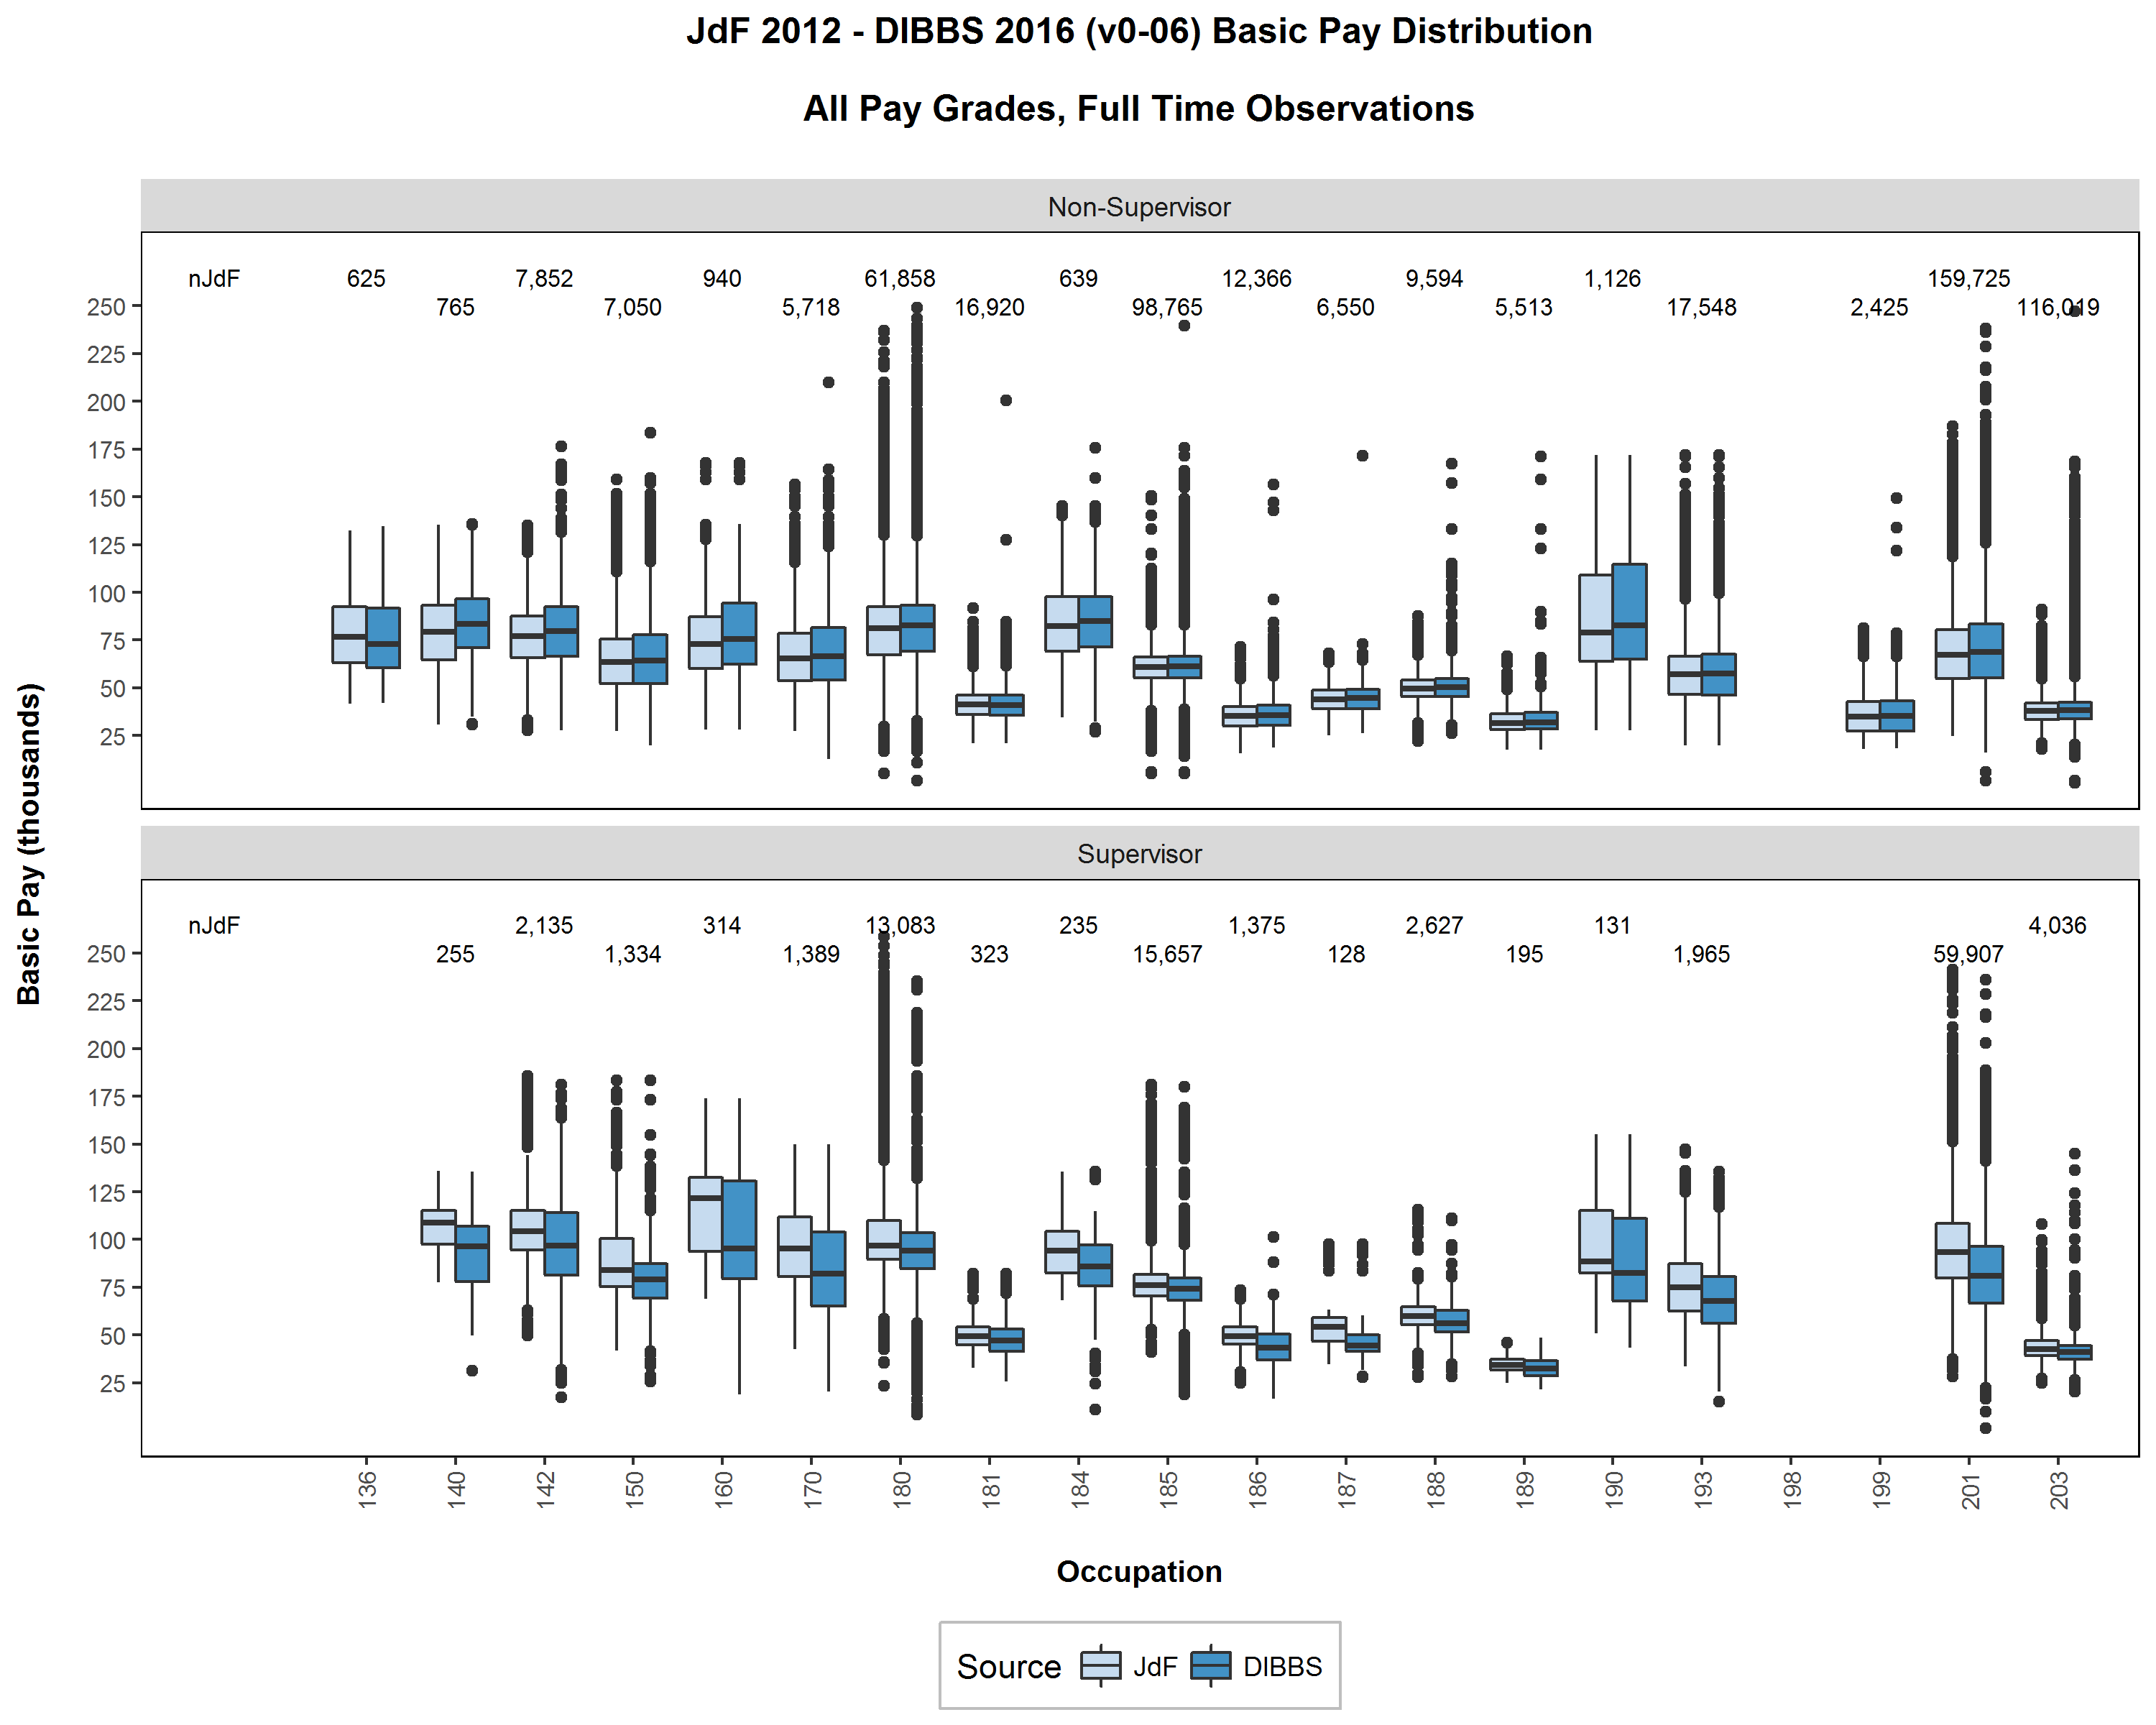
\includegraphics[width=6in, trim={0 1in 0 0.75in}, clip]{JdFDIBBSBasicPaySupervisoryStatusOccupation41.png}
        \caption{Occupations 0136 through 0203}
        \vspace{10pt}
    \end{subfigure}
    \begin{subfigure}{1\textwidth}
        \centering
        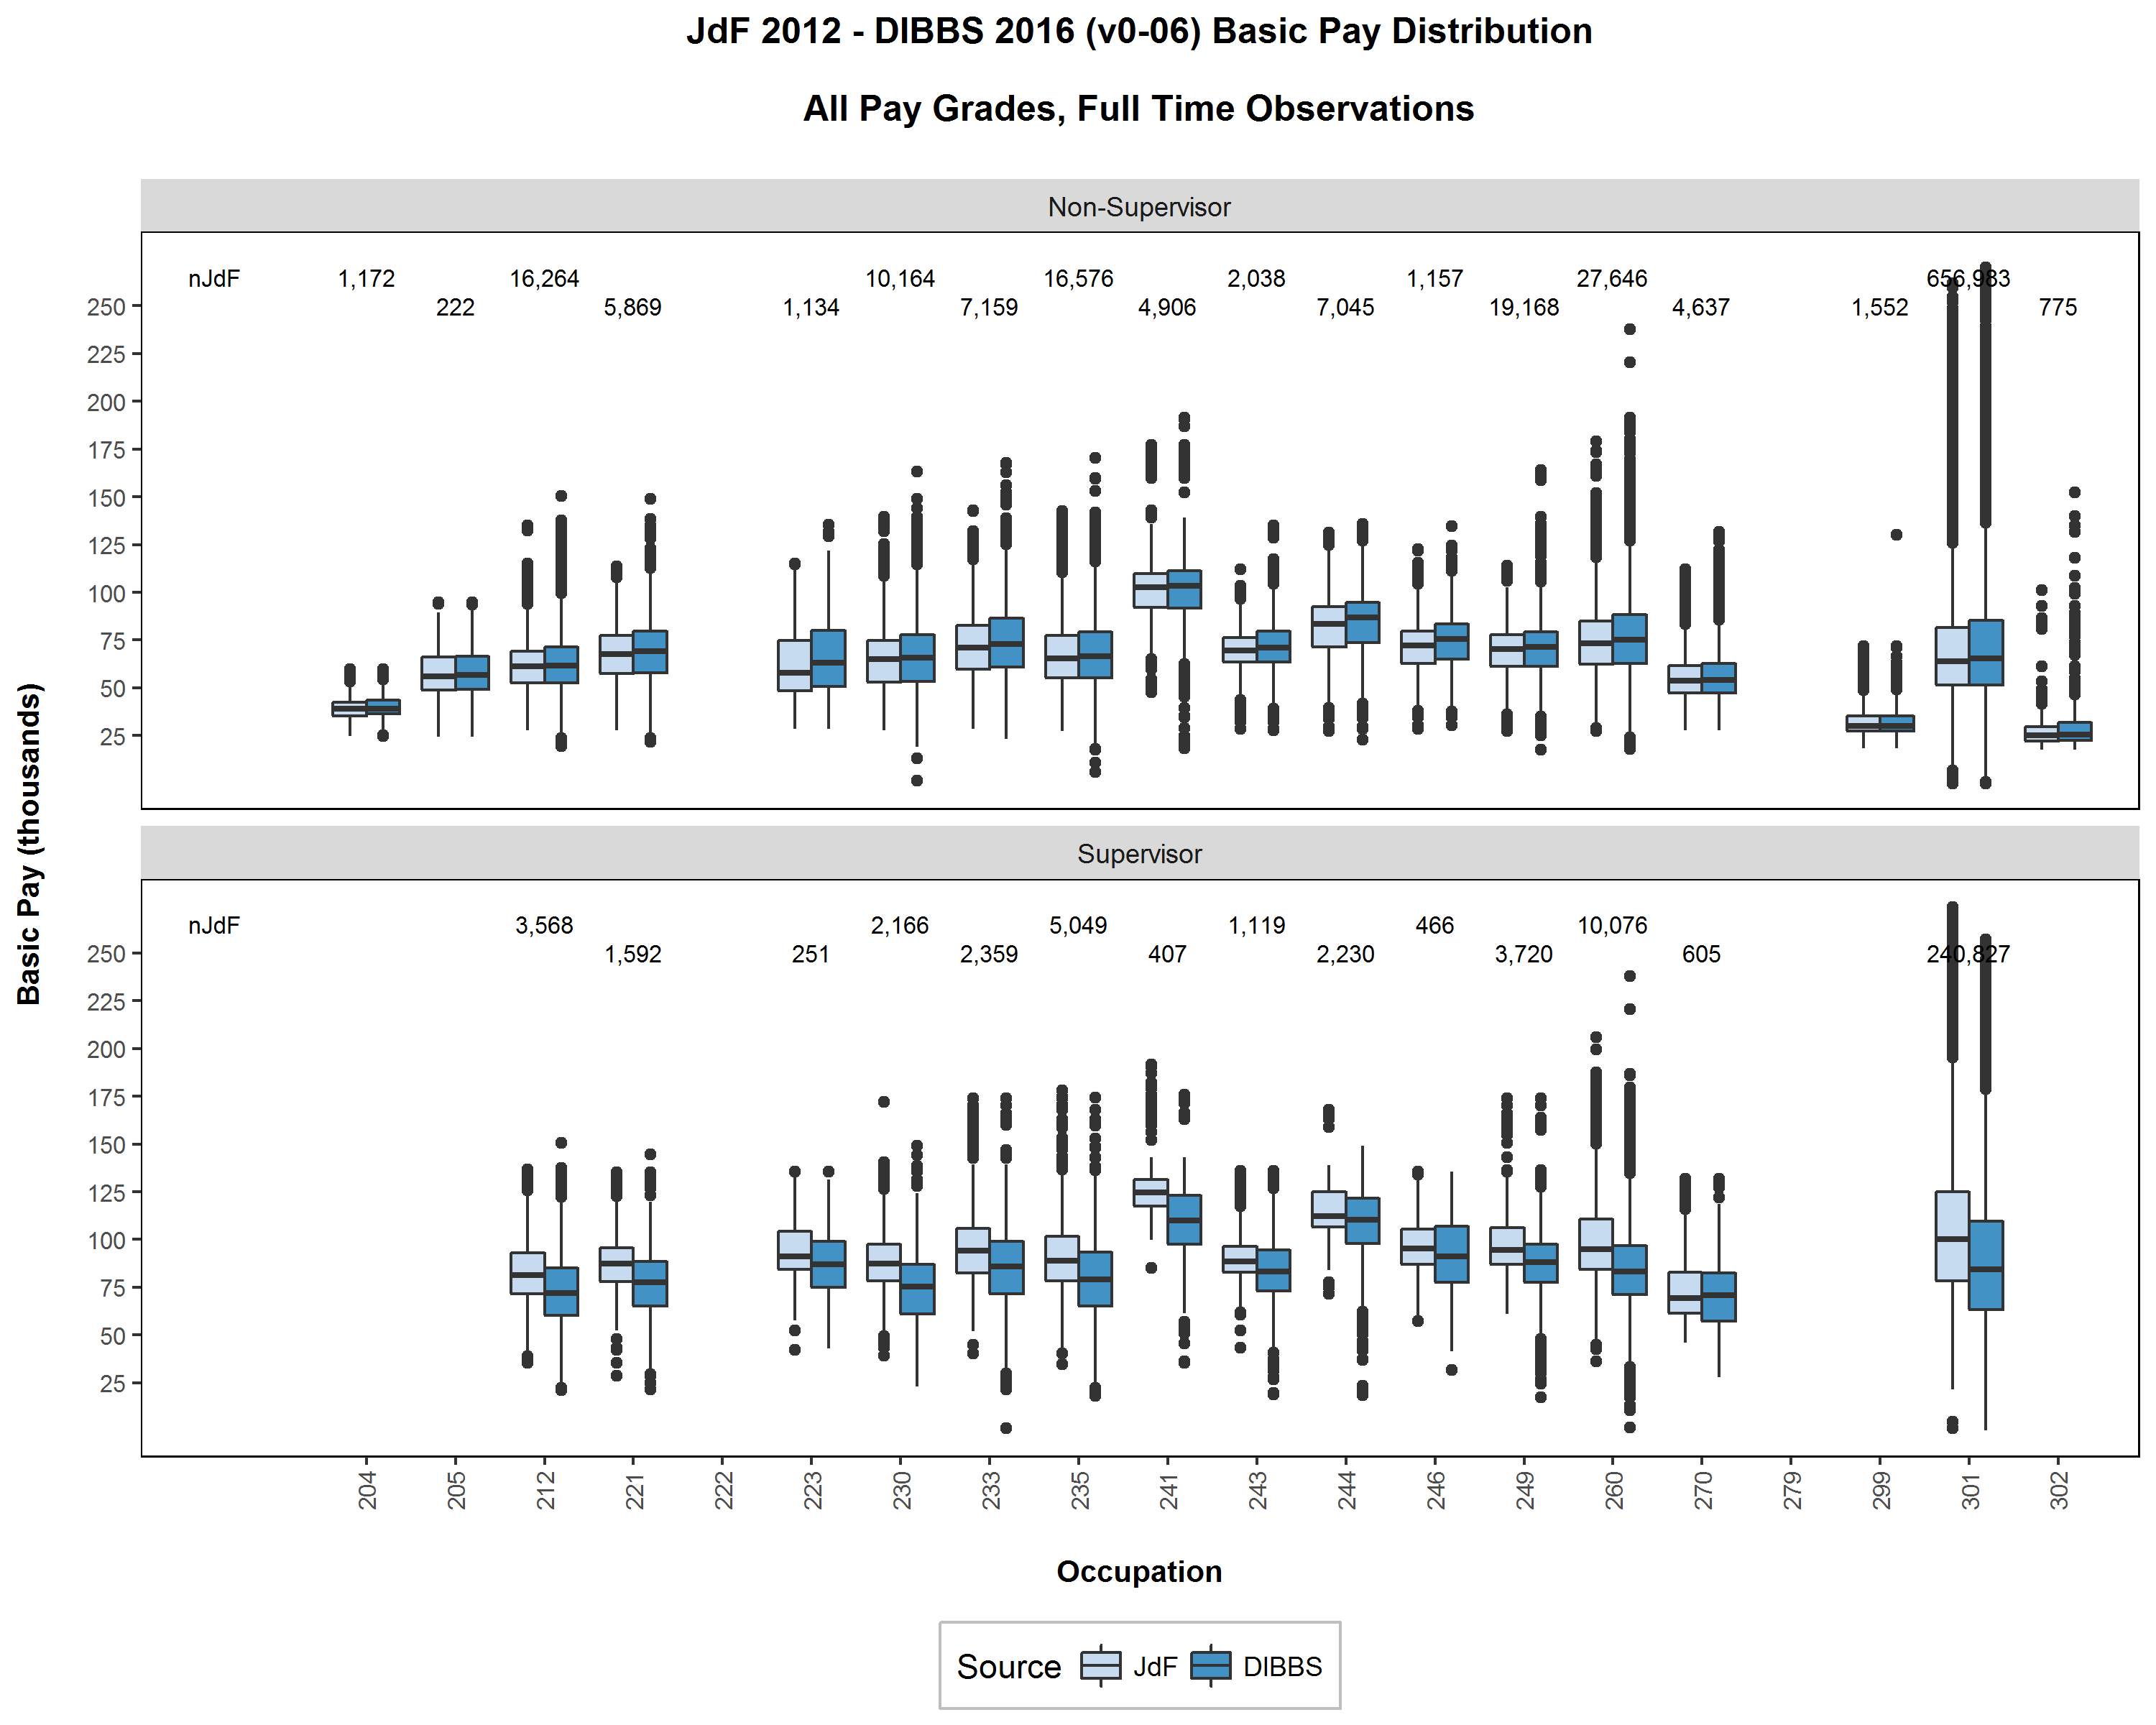
\includegraphics[width=6in, trim={0 1in 0 0.75in}, clip]{JdFDIBBSBasicPaySupervisoryStatusOccupation61.png}
        \caption{Occupations 0204 through 0302}
        \vspace{10pt}
    \end{subfigure}
    \caption{Basic pay distribution by occupation and supervisor status.  All agencies combined.  Authentic boxes on left, synthetic on right.}
    \label{figure:JdFDIBBSBasicPaySupervisoryStatusOccupation2}
\end{figure}

\clearpage

\begin{figure}[h]
    \centering
    \begin{subfigure}{1\textwidth}
        \centering
        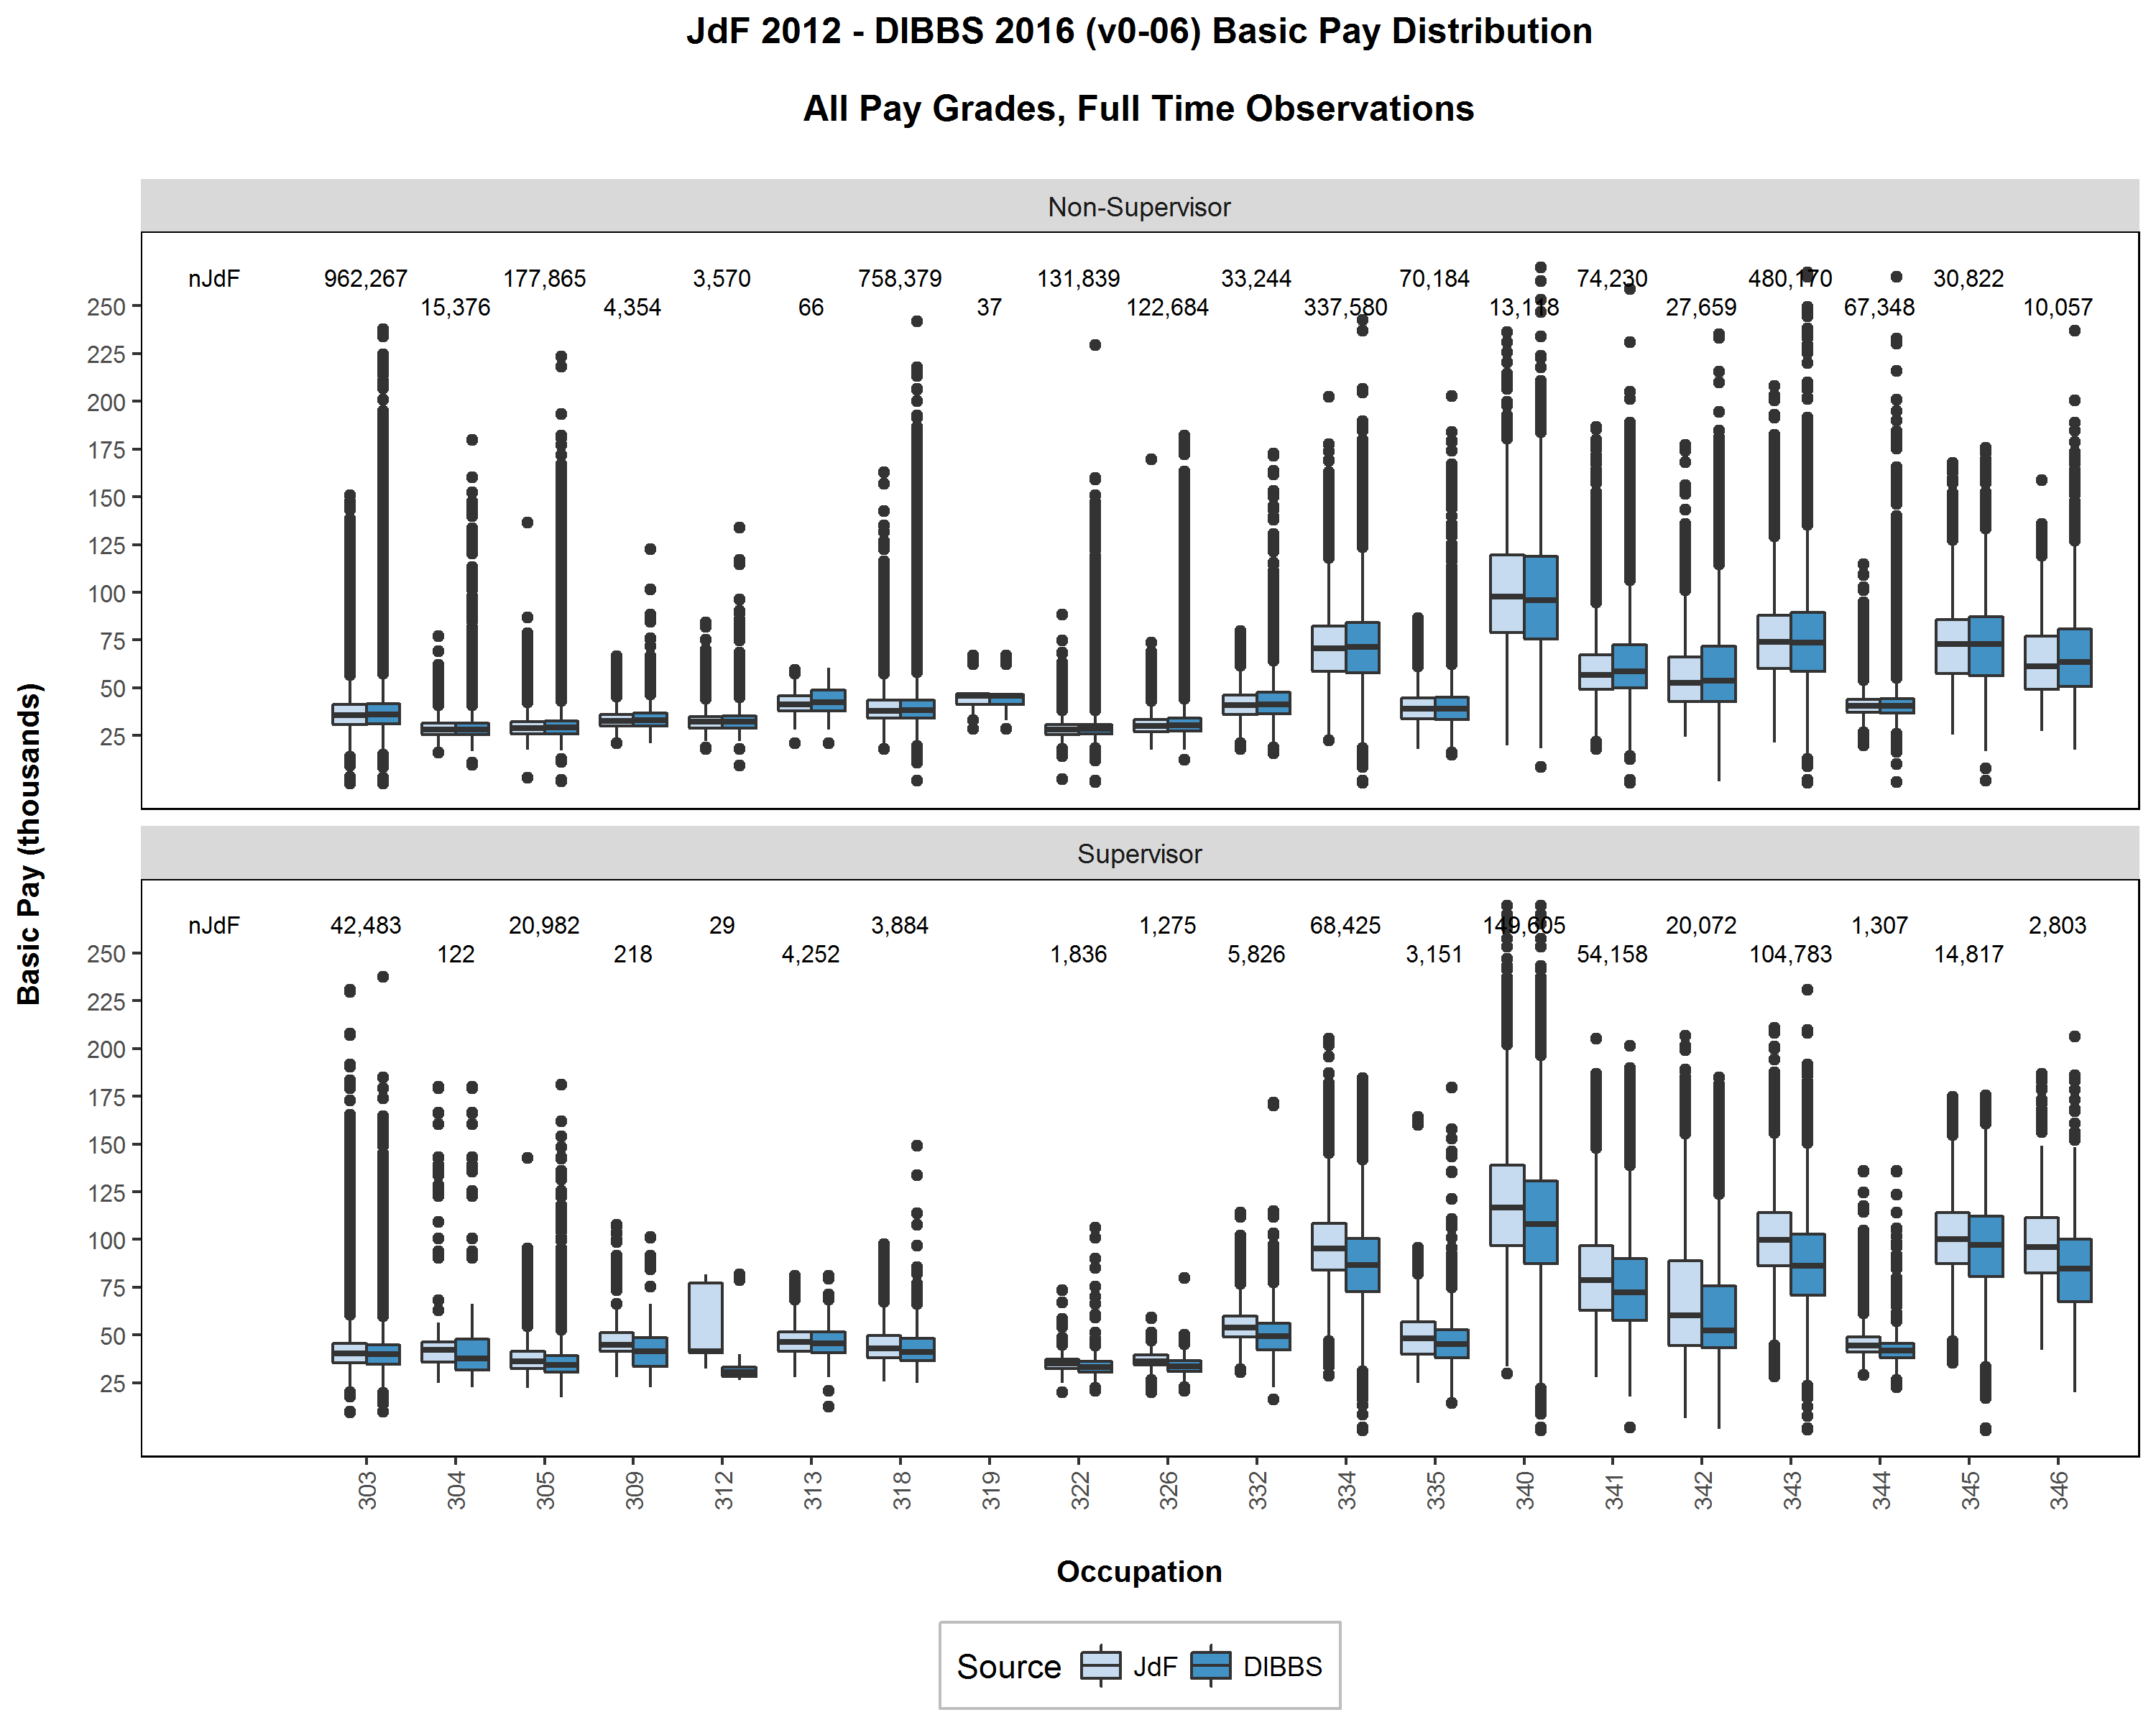
\includegraphics[width=6in, trim={0 1in 0 0.75in}, clip]{JdFDIBBSBasicPaySupervisoryStatusOccupation81.png}
        \caption{Occupations 0303 through 0346}
        \vspace{10pt}
    \end{subfigure}
    \begin{subfigure}{1\textwidth}
        \centering
        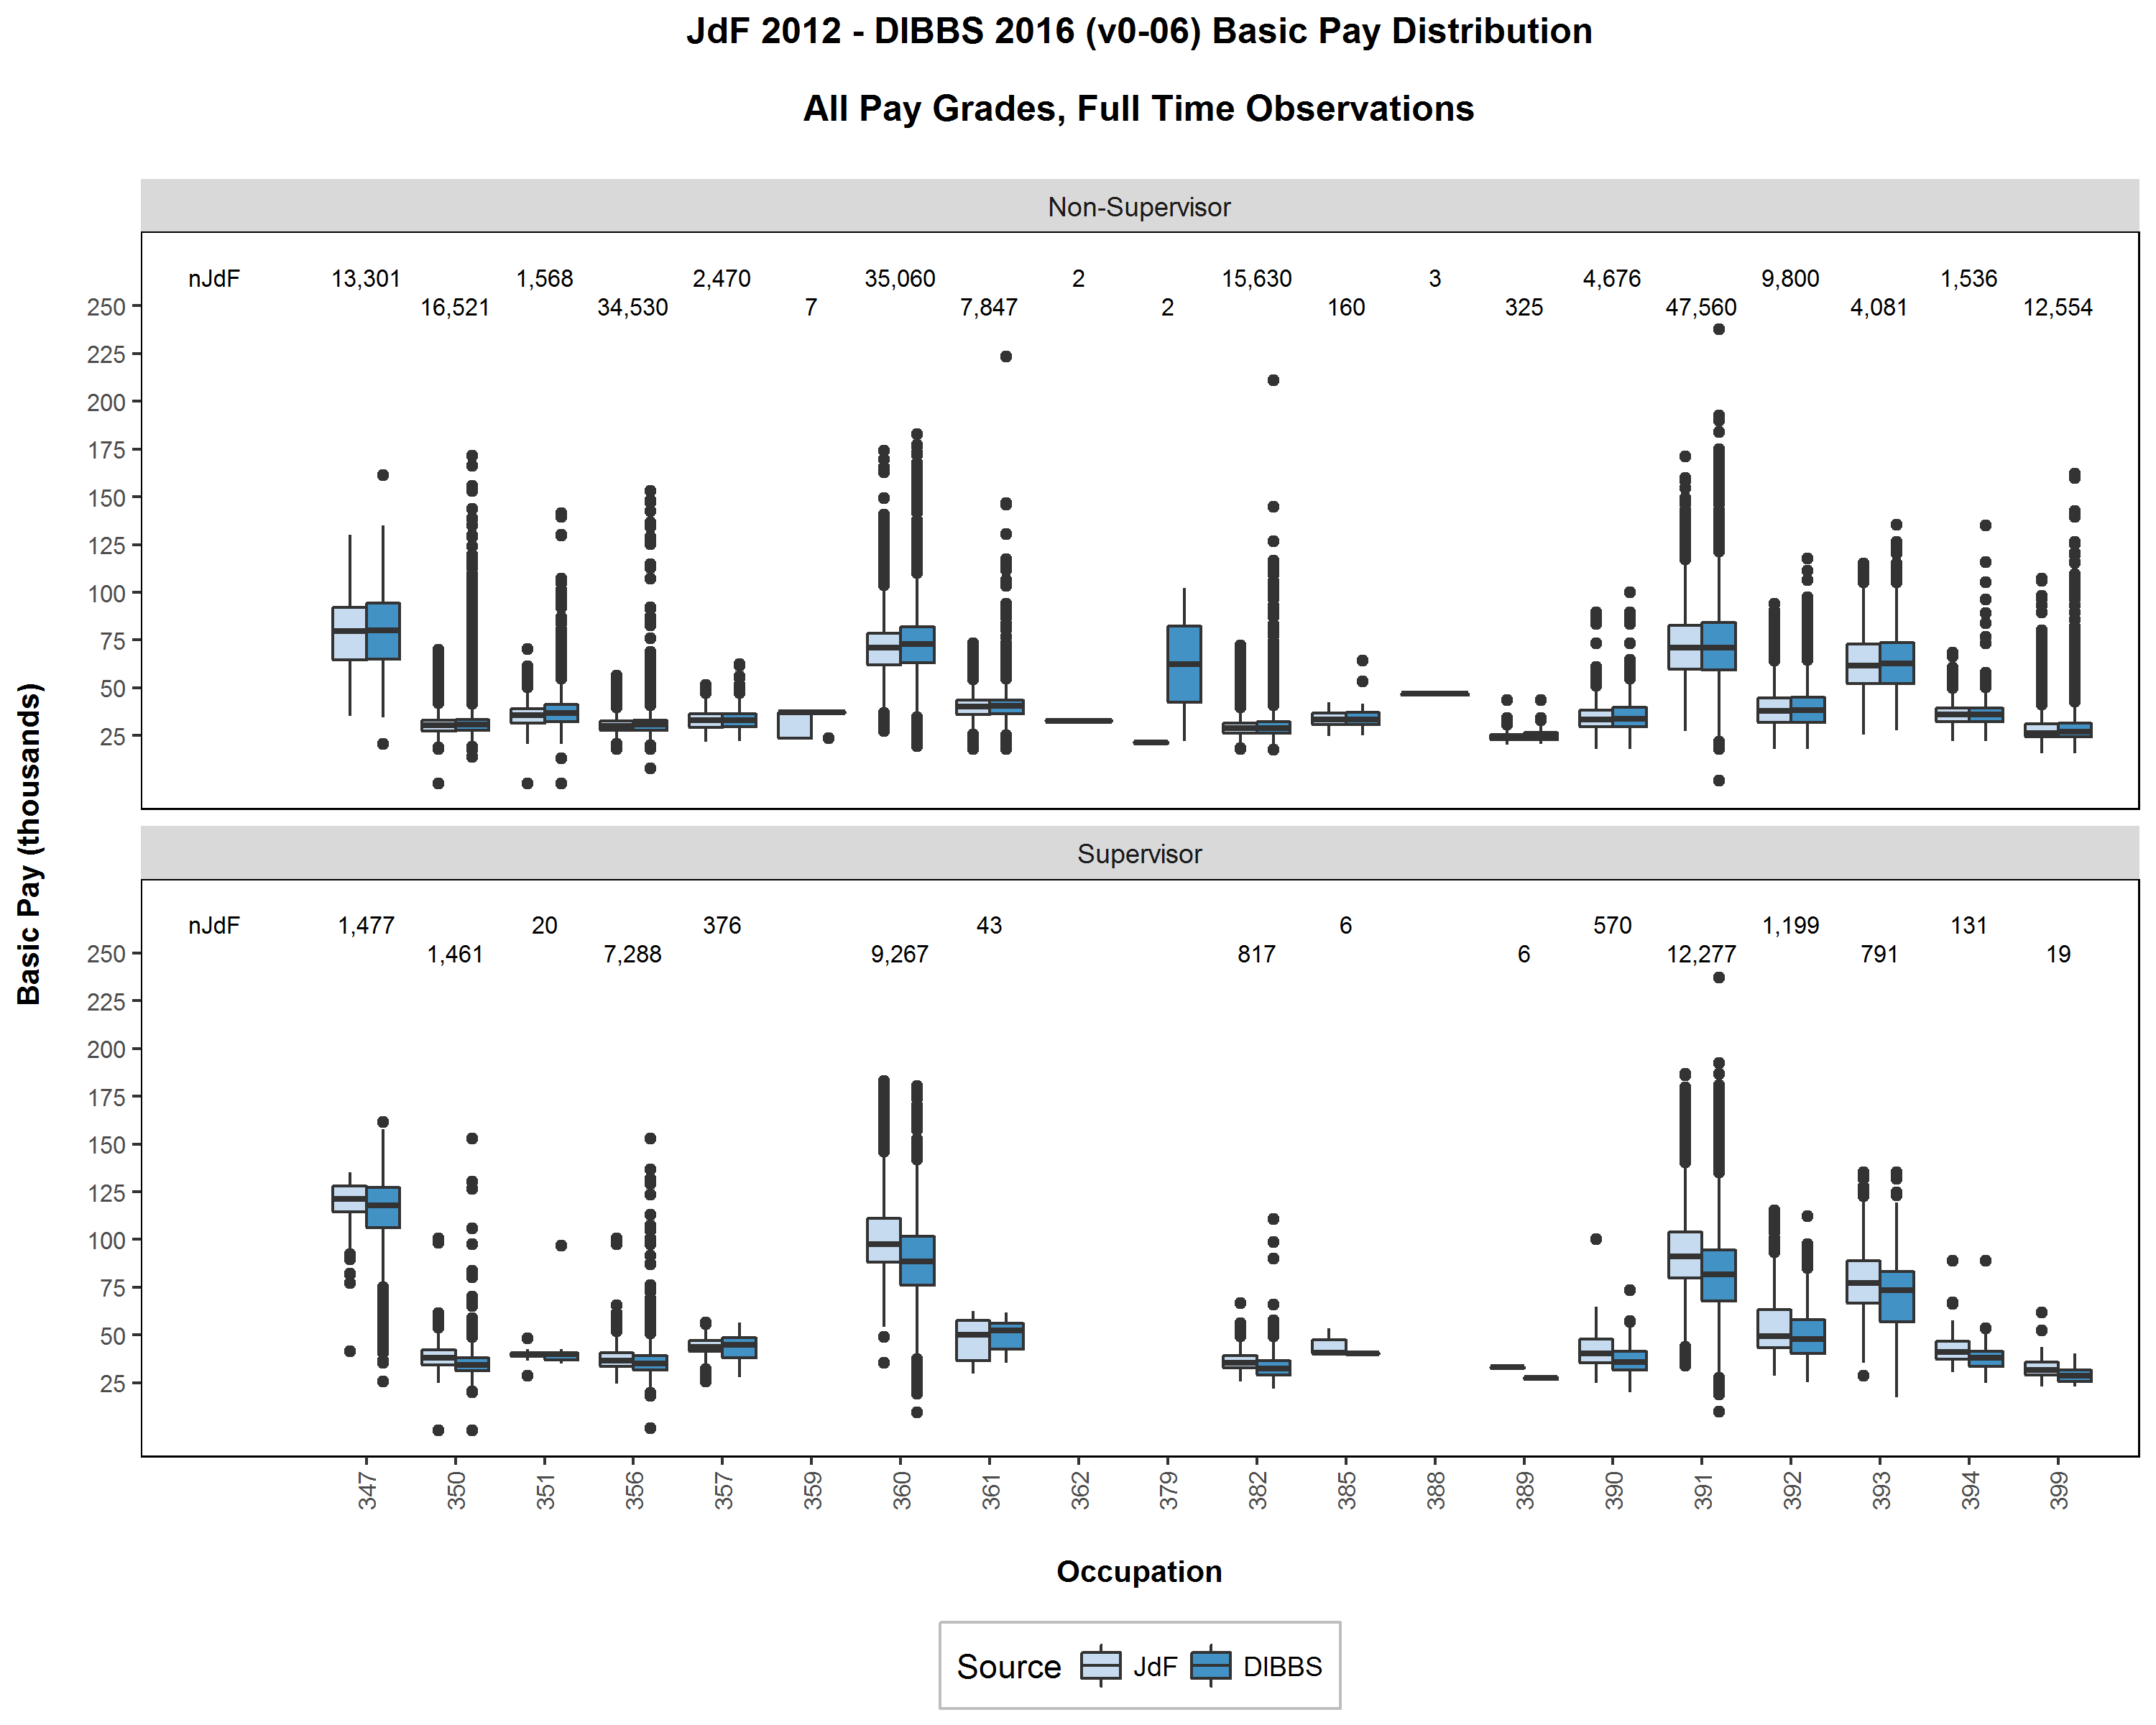
\includegraphics[width=6in, trim={0 1in 0 0.75in}, clip]{JdFDIBBSBasicPaySupervisoryStatusOccupation101.png}
        \caption{Occupations 0347 through 0399}
        \vspace{10pt}
    \end{subfigure}
    \caption{Basic pay distribution by occupation and supervisor status.  All agencies combined.  Authentic boxes on left, synthetic on right.}
    \label{figure:JdFDIBBSBasicPaySupervisoryStatusOccupation3}
\end{figure}

\begin{figure}[h]
    \centering
    \begin{subfigure}{1\textwidth}
        \centering
        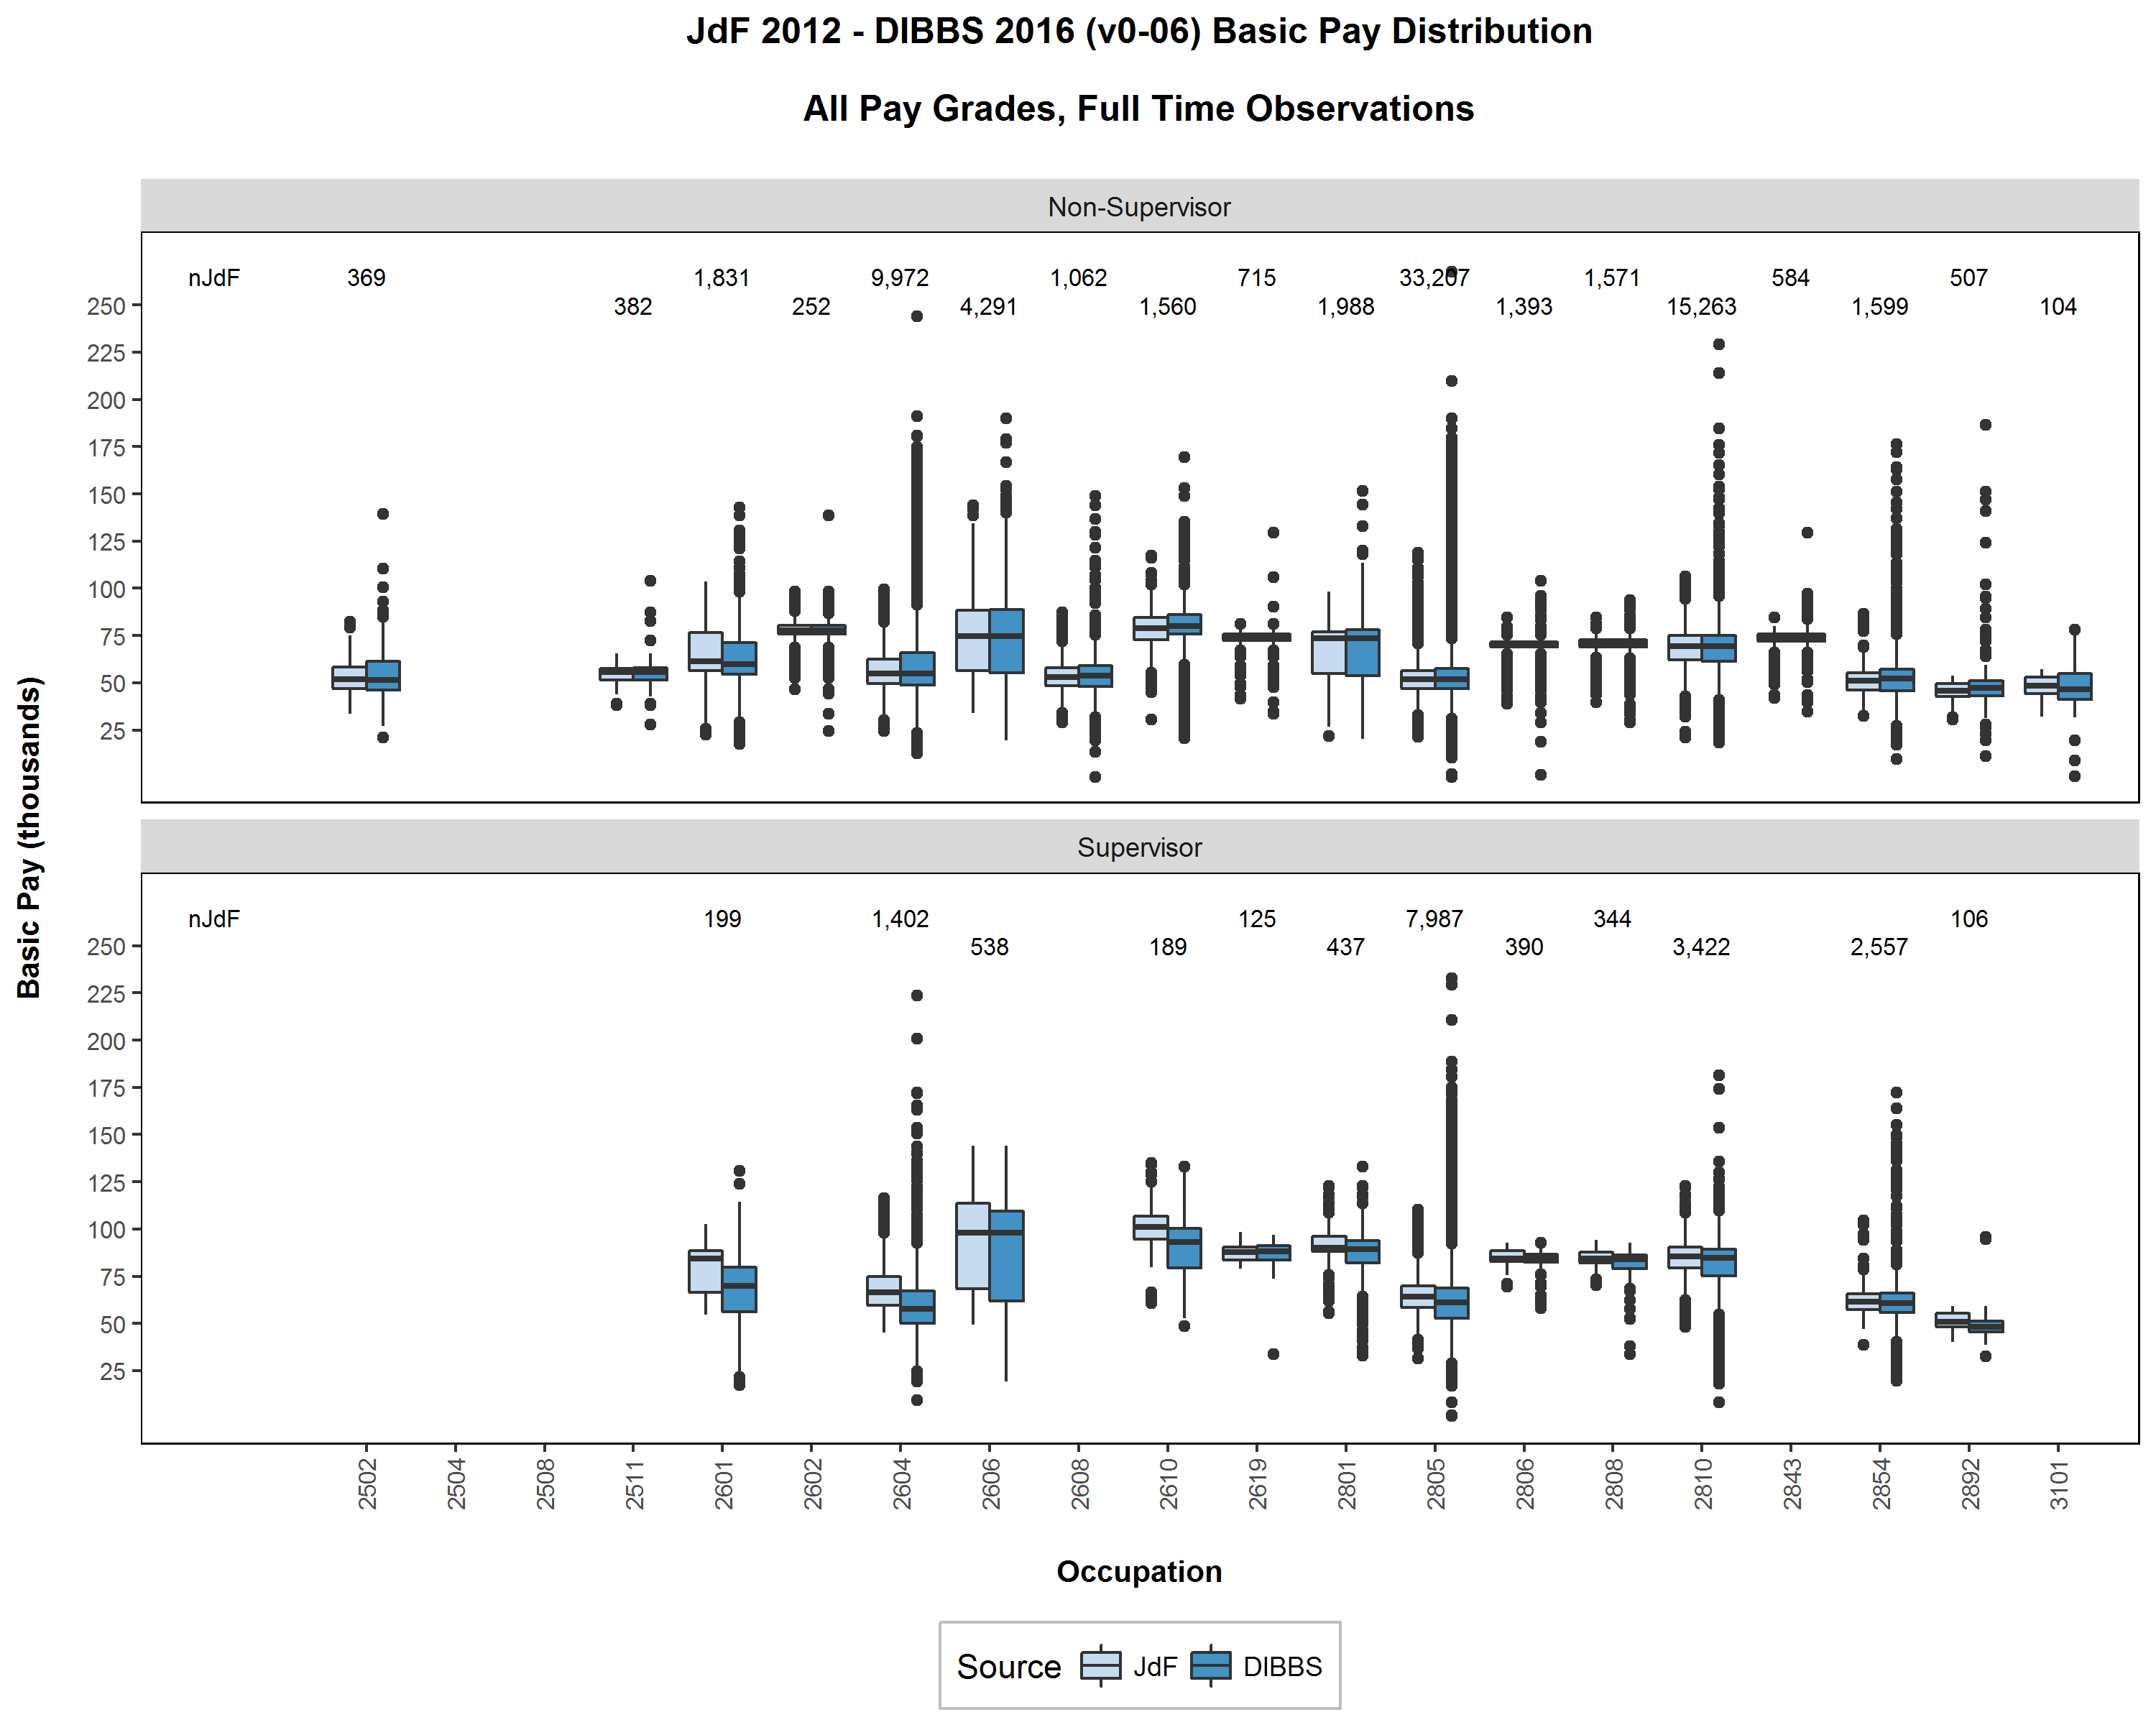
\includegraphics[width=6in, trim={0 1in 0 0.75in}, clip]{JdFDIBBSBasicPaySupervisoryStatusOccupation481.png}
        \caption{Occupations 2502 through 3101 (trades)}
        \vspace{10pt}
    \end{subfigure}
    \begin{subfigure}{1\textwidth}
        \centering
        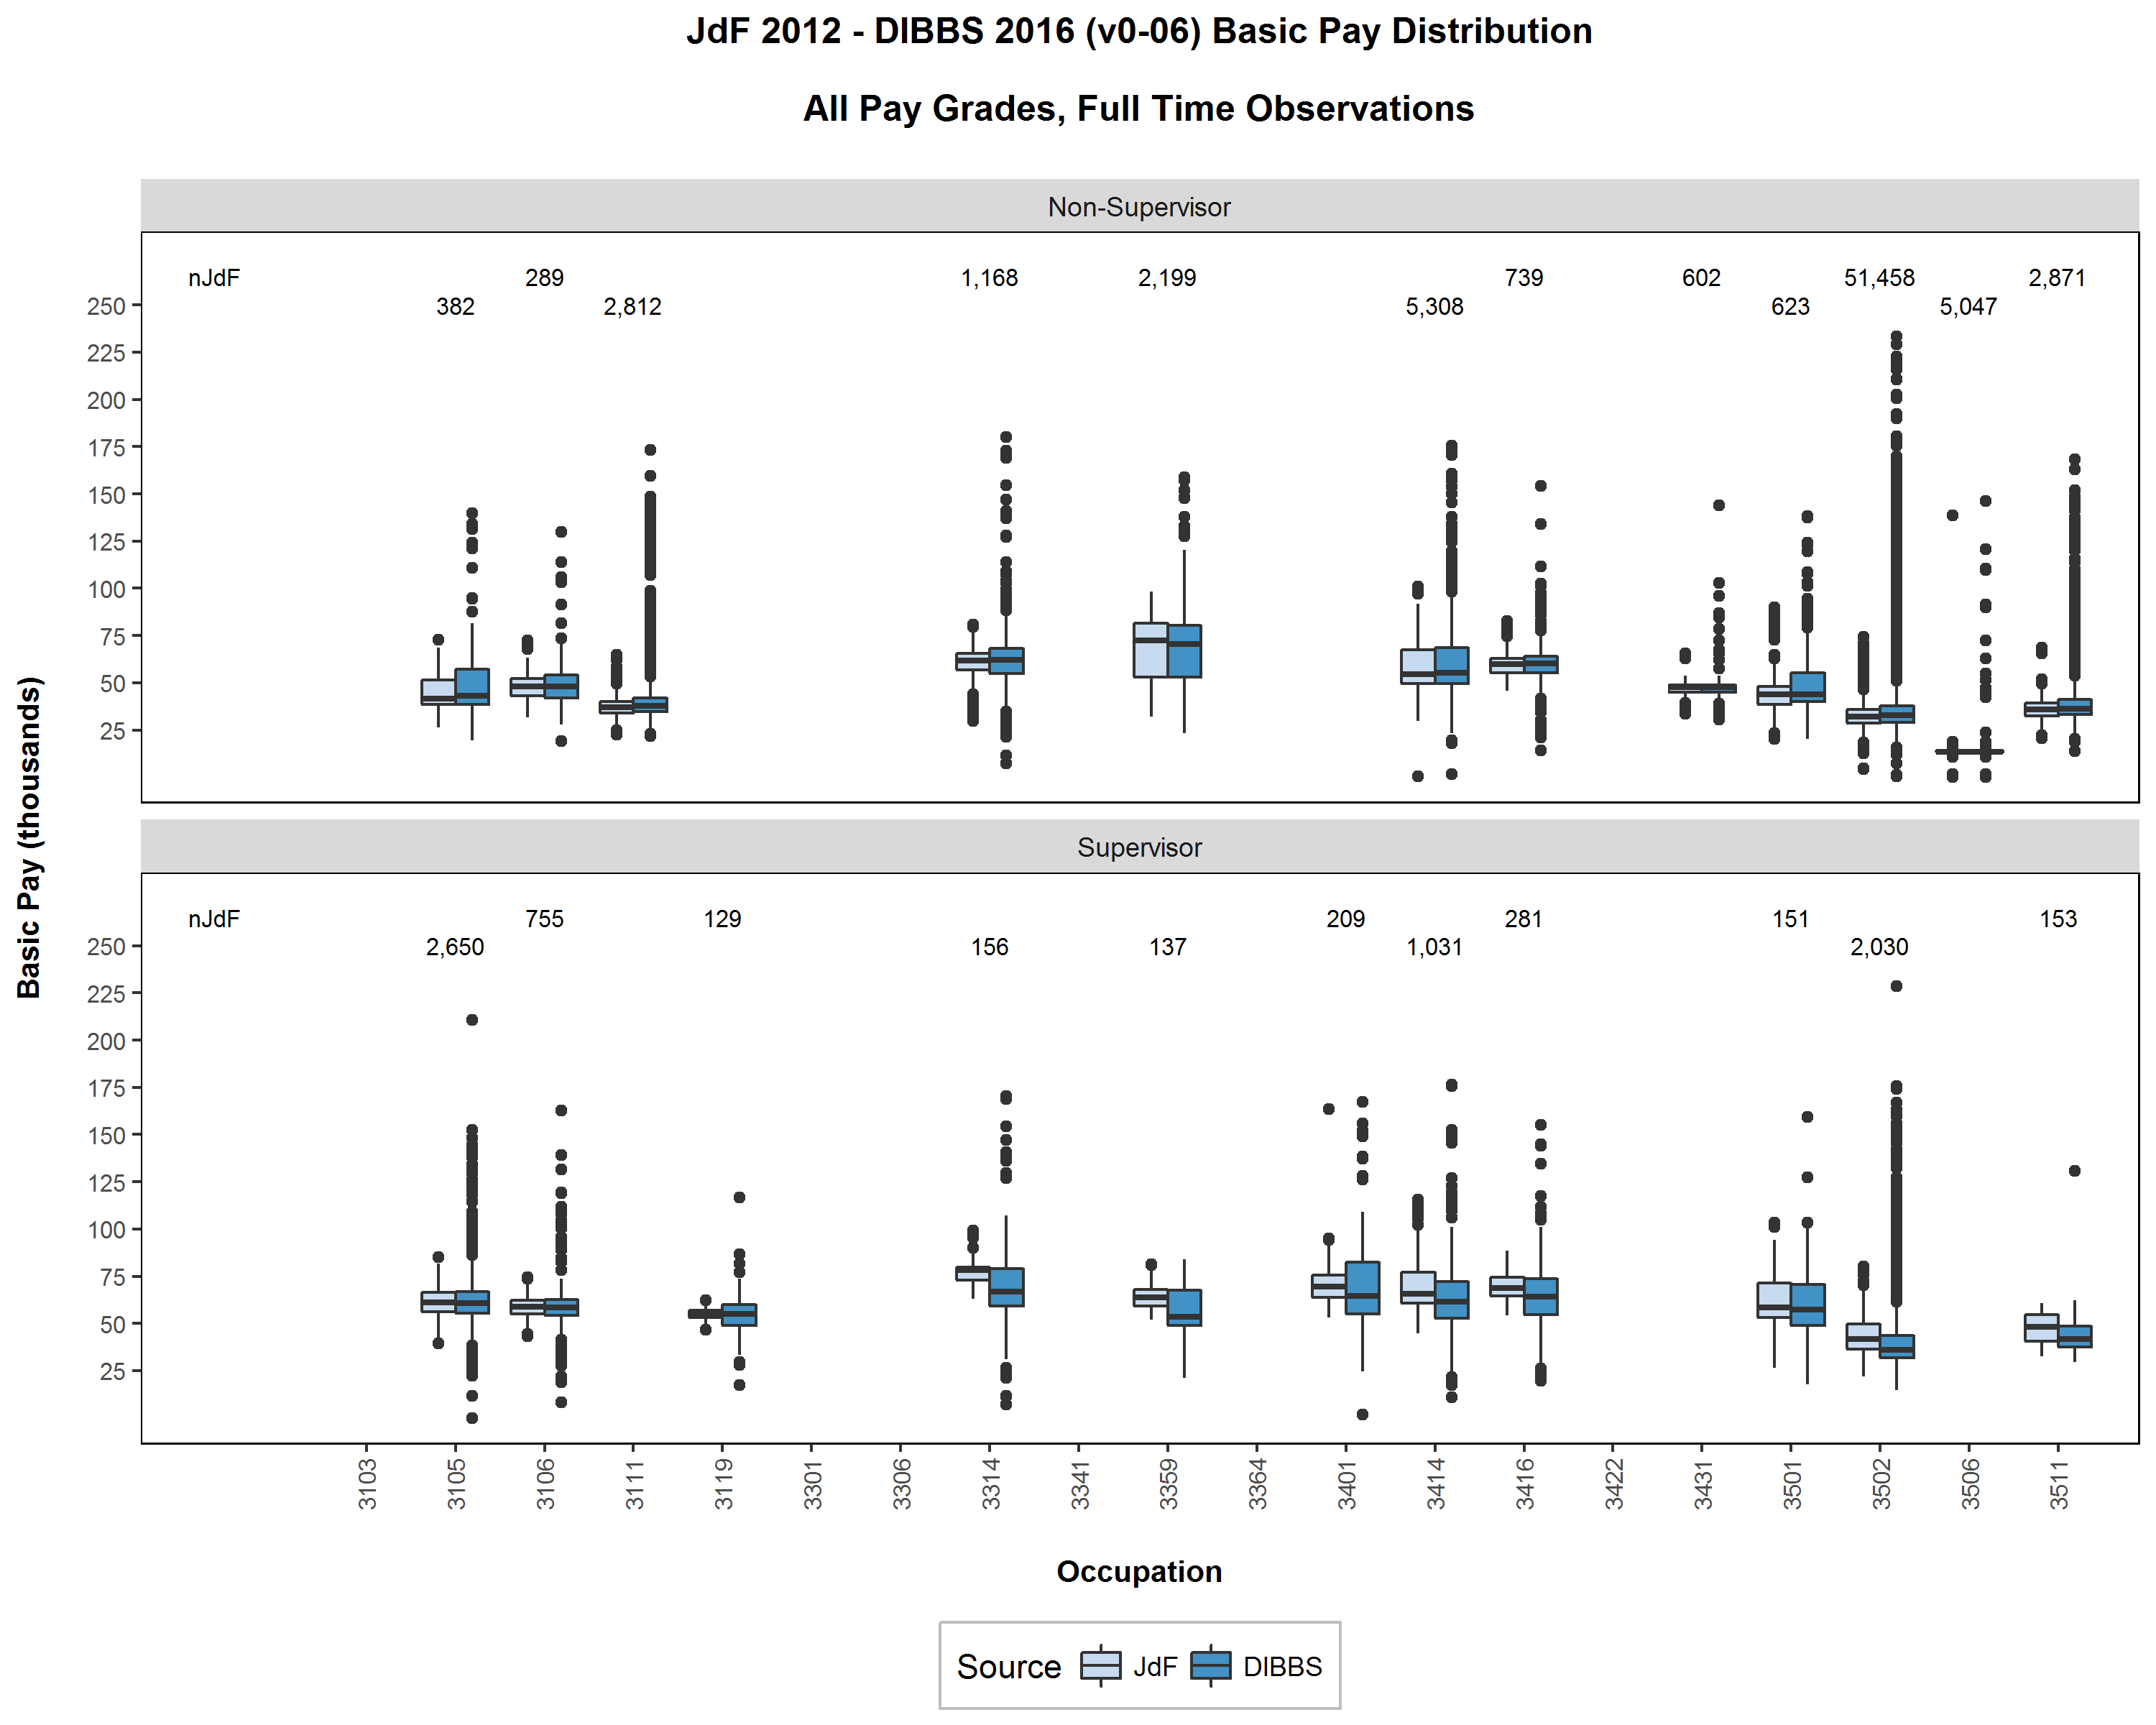
\includegraphics[width=6in, trim={0 1in 0 0.75in}, clip]{JdFDIBBSBasicPaySupervisoryStatusOccupation501.png}
        \caption{Occupations 3103 through 3511 (trades)}
        \vspace{10pt}
    \end{subfigure}
    \caption{Basic pay distribution by occupation and supervisor status.  All agencies combined.  Authentic boxes on left, synthetic on right.}
    \label{figure:JdFDIBBSBasicPaySupervisoryStatusOccupation4}
\end{figure}

\clearpage

\begin{figure}[h]
    \centering
    \begin{subfigure}{1\textwidth}
        \centering
        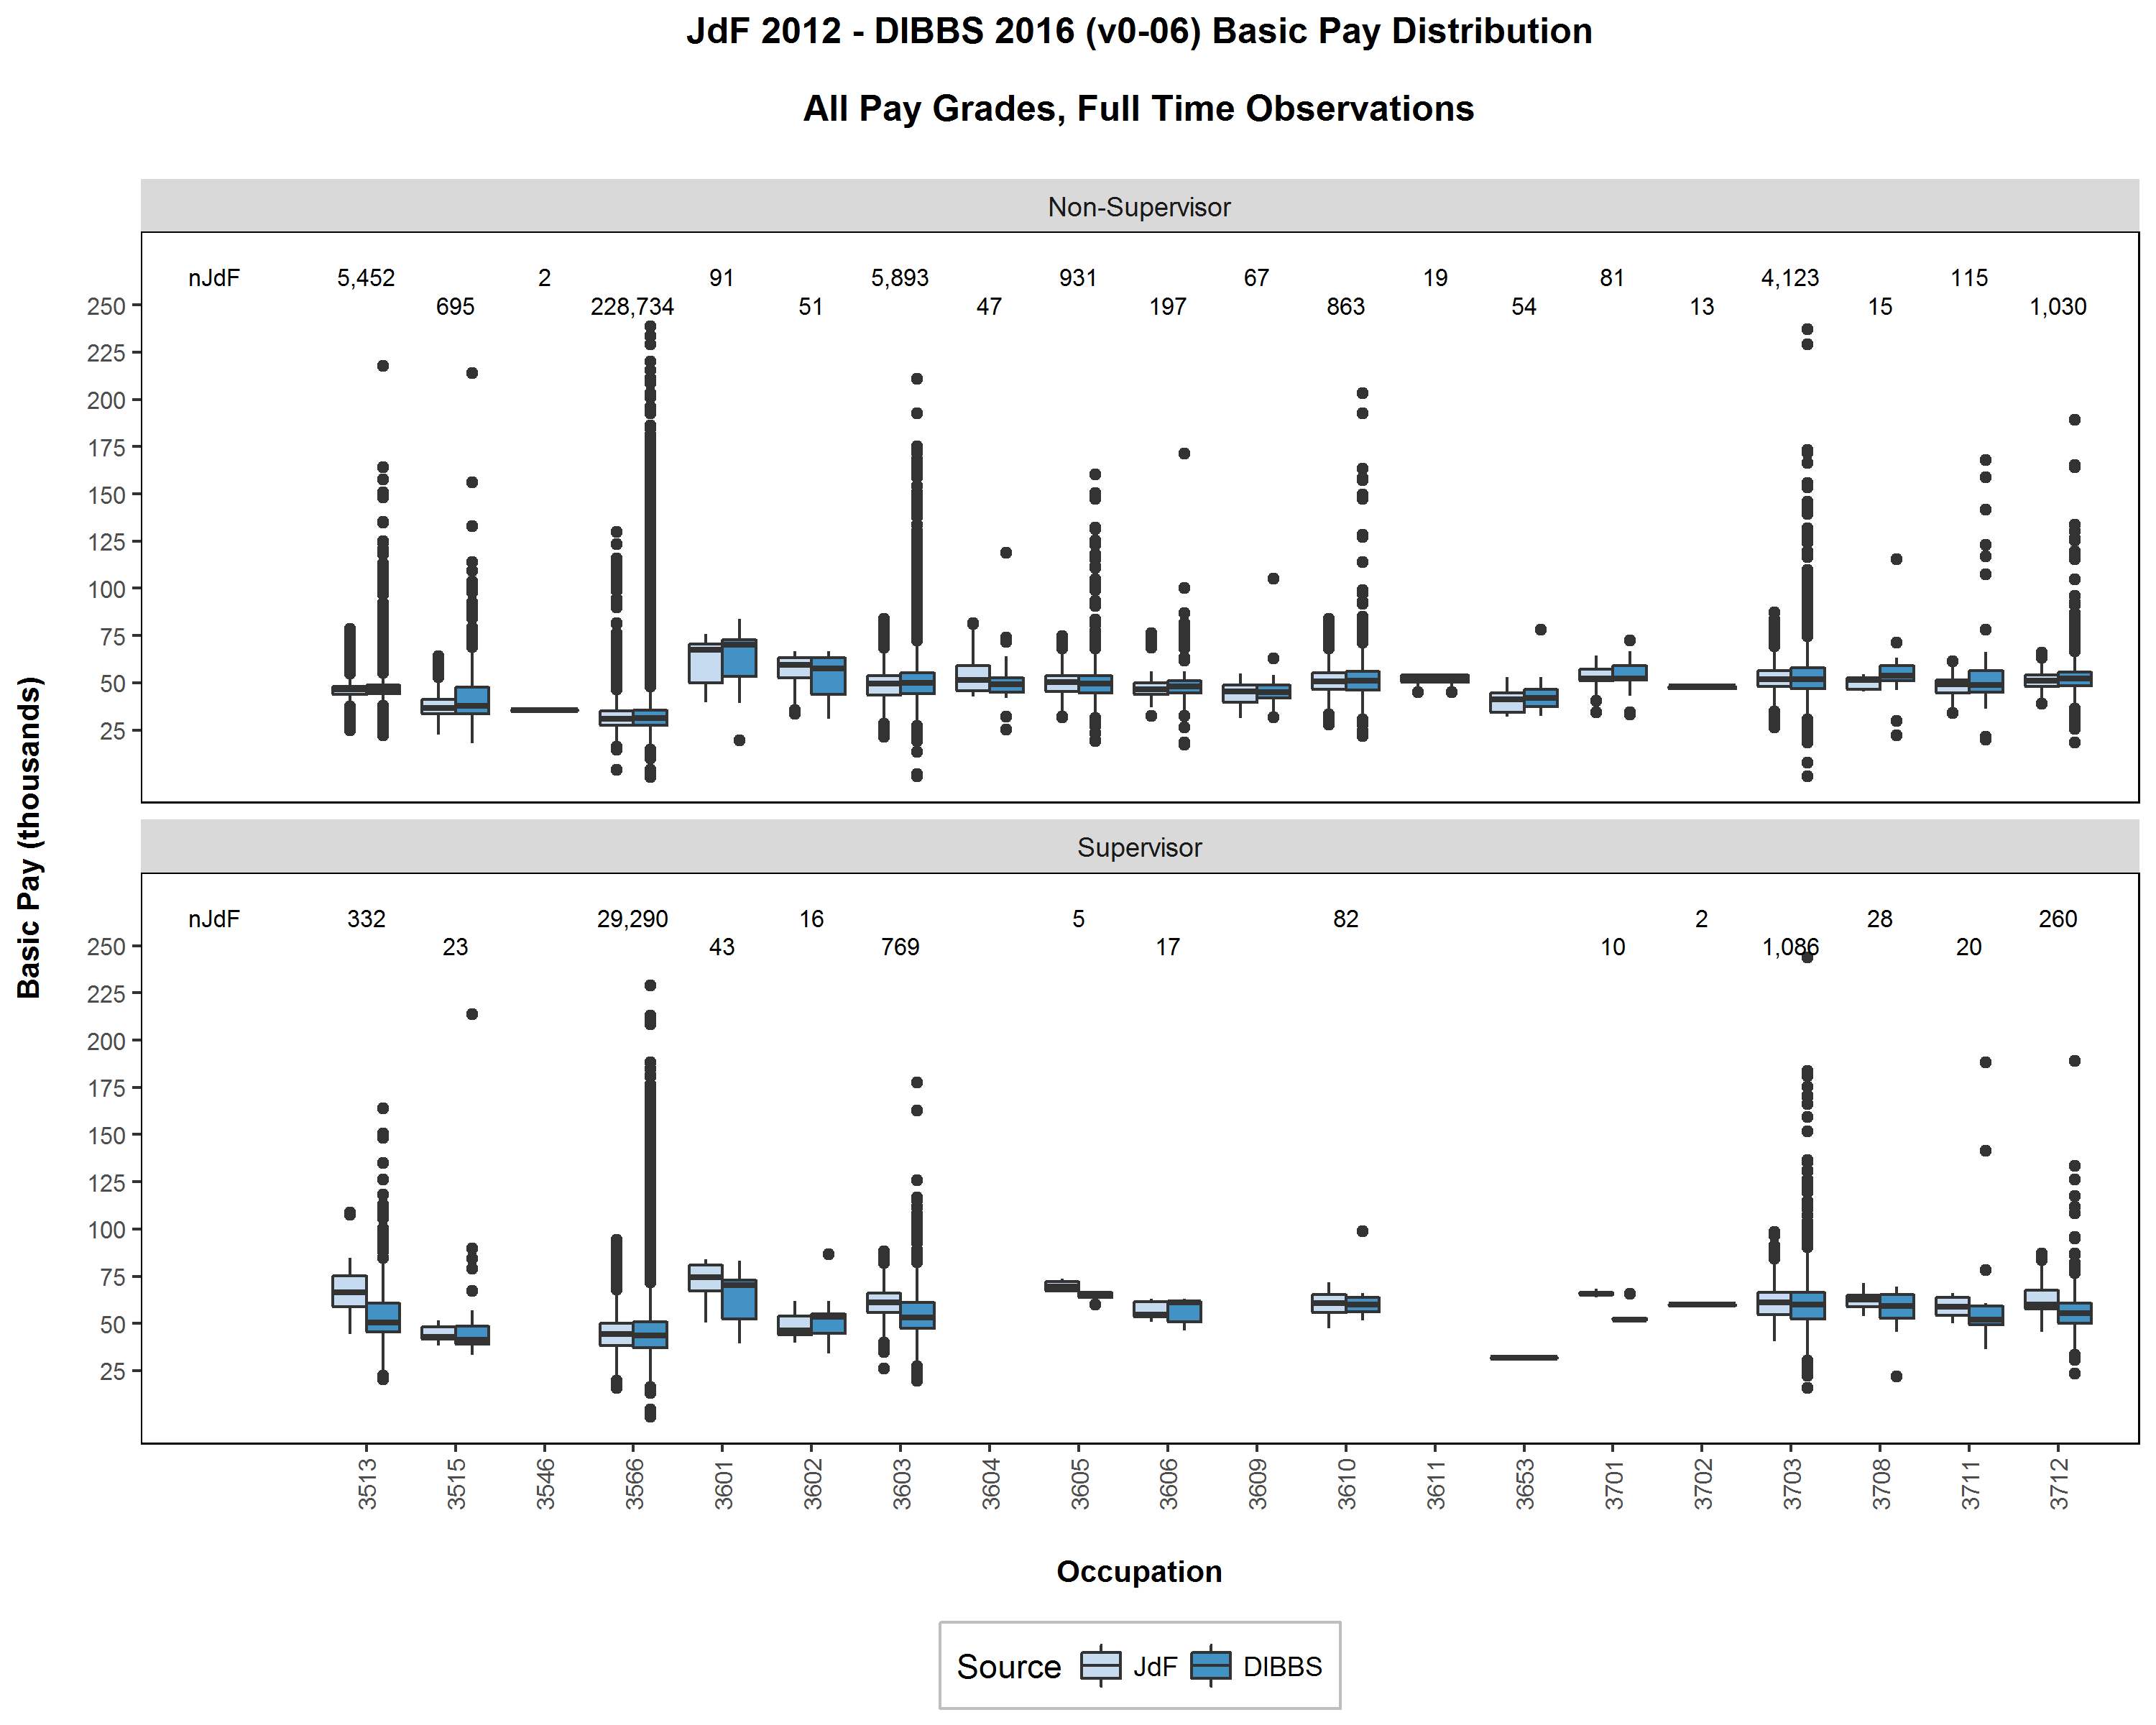
\includegraphics[width=6in, trim={0 1in 0 0.75in}, clip]{JdFDIBBSBasicPaySupervisoryStatusOccupation521.png}
        \caption{Occupations 3513 through 3712 (trades)}
        \vspace{10pt}
    \end{subfigure}
    \begin{subfigure}{1\textwidth}
        \centering
        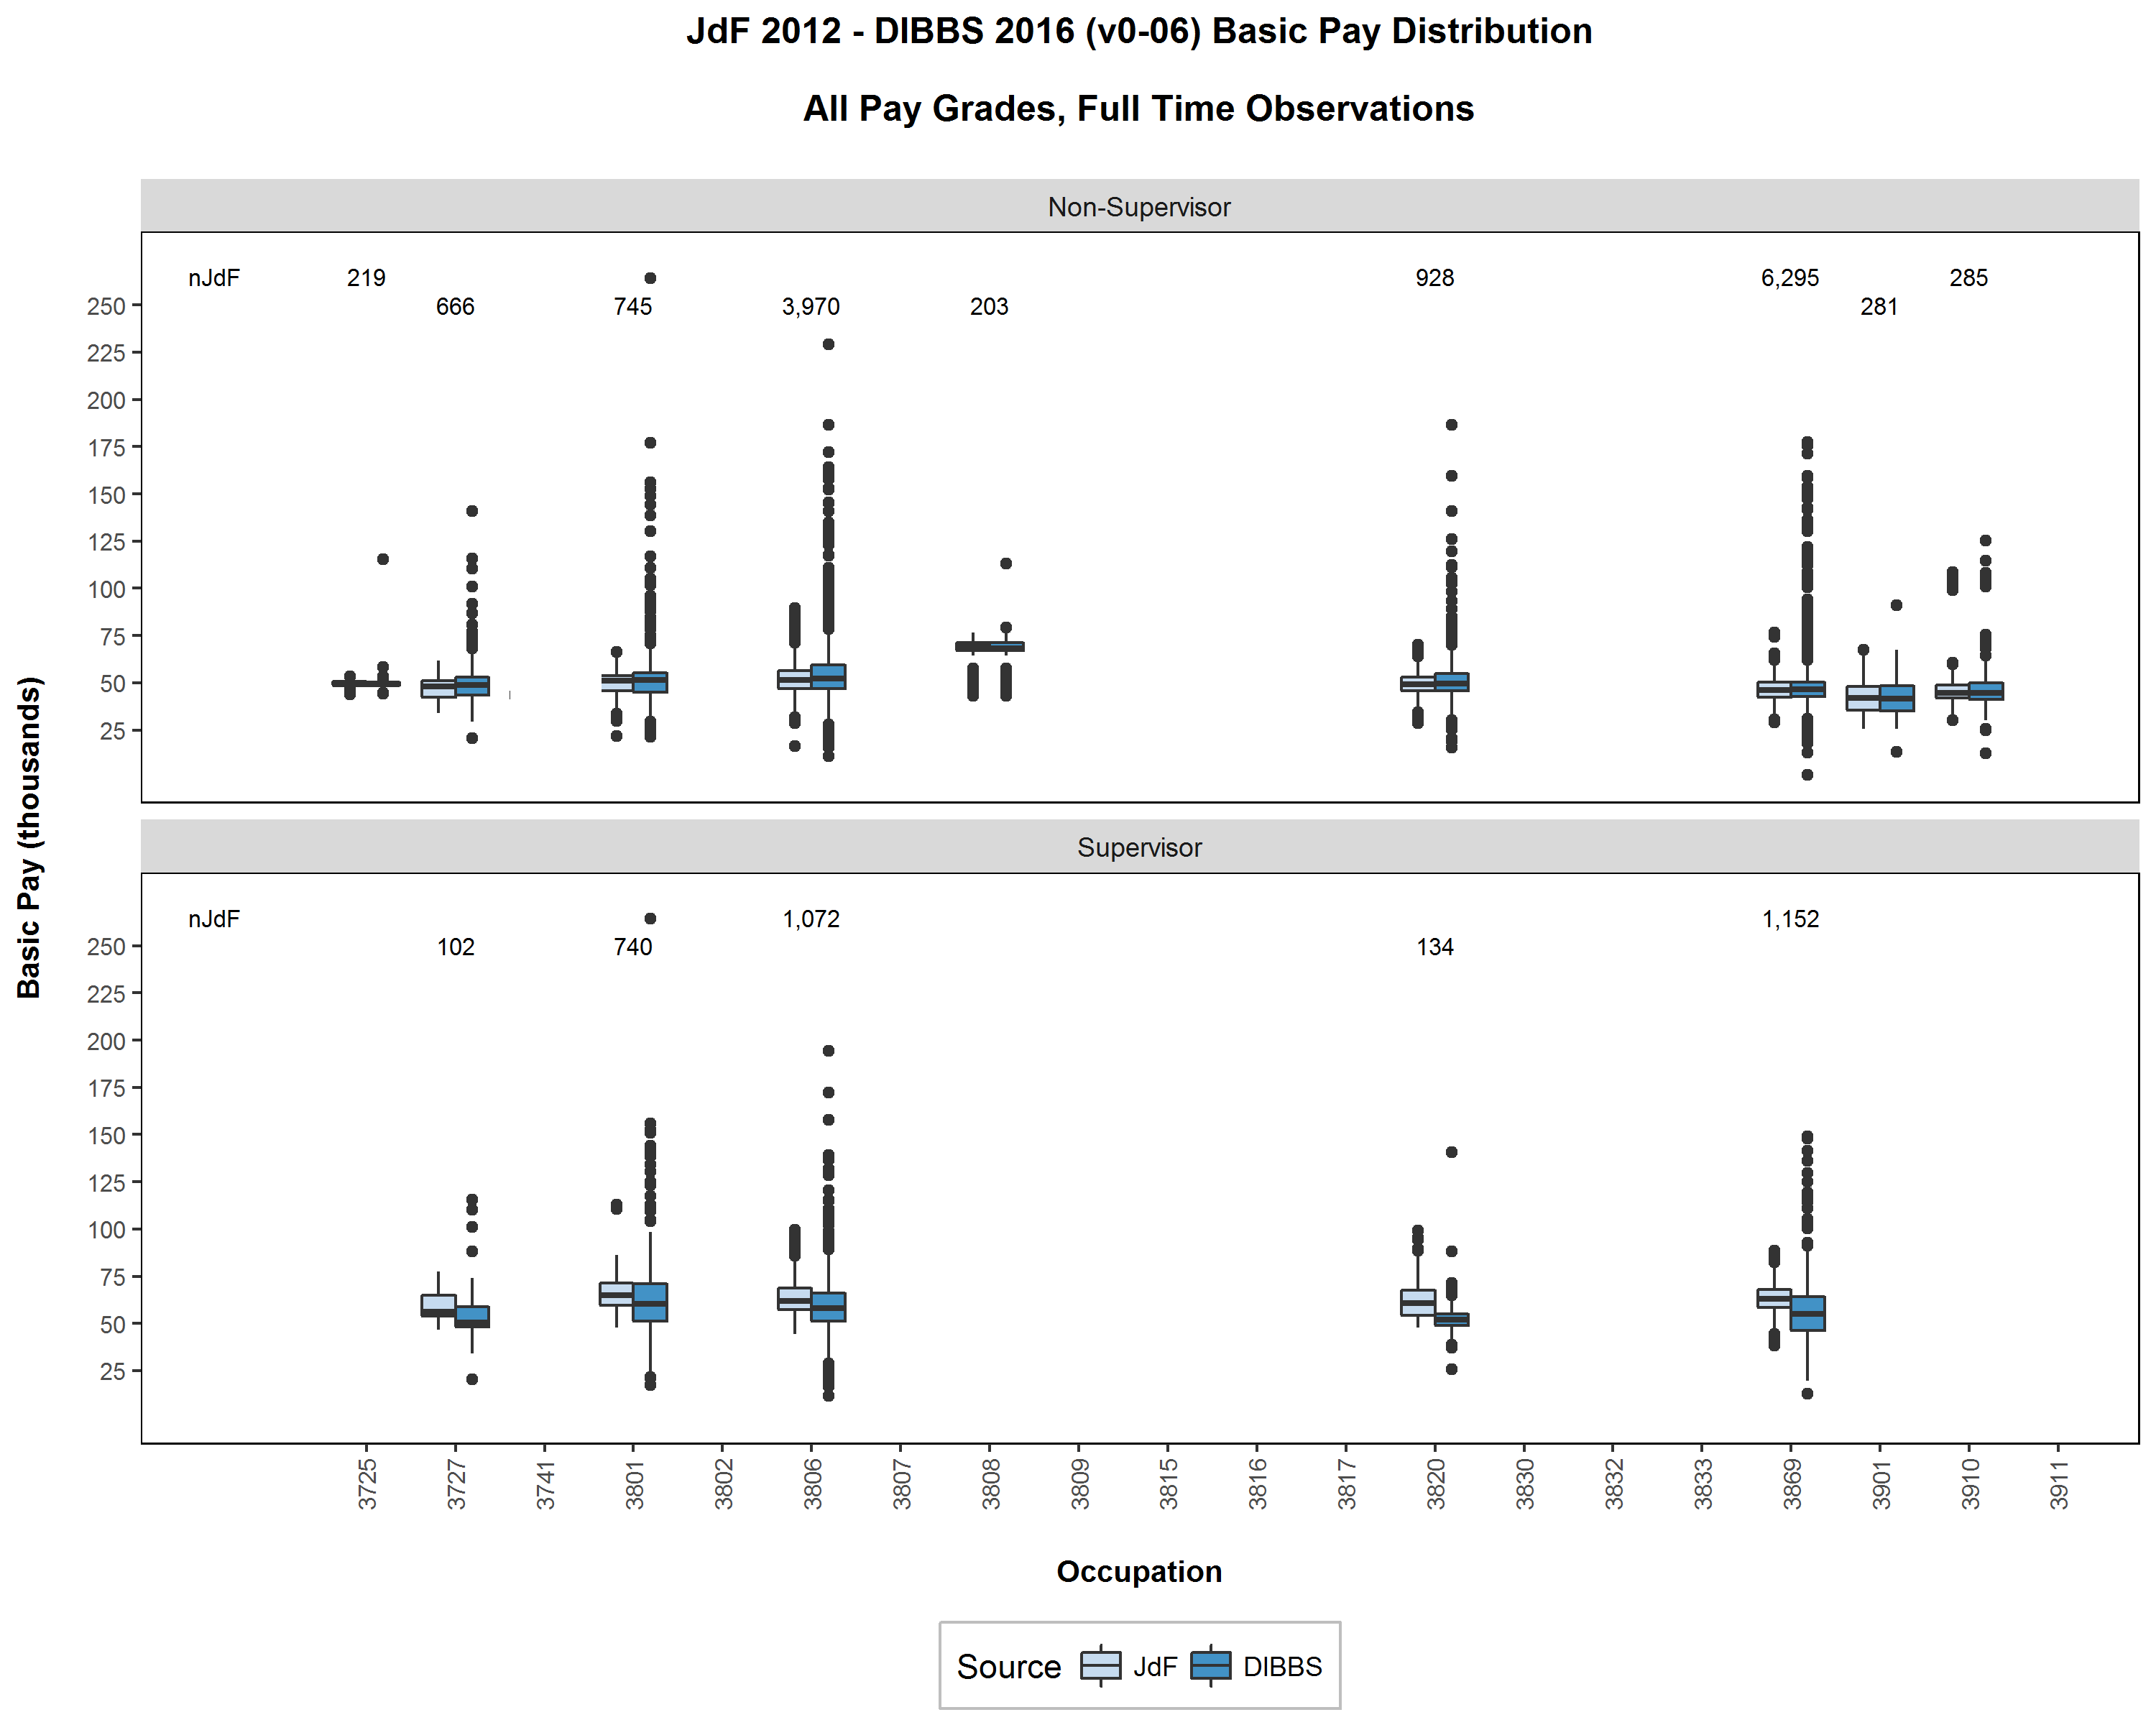
\includegraphics[width=6in, trim={0 1in 0 0.75in}, clip]{JdFDIBBSBasicPaySupervisoryStatusOccupation541.png}
        \caption{Occupations 3725 through 3911 (trades}
        \vspace{10pt}
    \end{subfigure}
    \caption{Basic pay distribution by occupation and supervisor status.  All agencies combined.  Authentic boxes on left, synthetic on right.}
    \label{figure:JdFDIBBSBasicPaySupervisoryStatusOccupation5}
\end{figure}

\clearpage

MEAN LOG(BASIC PAY) BY GENDER, RACE, AND YEAR\\

The relationship of mean basic basic pay to joint combinations of sex, race, and year is important in human capital research and must be maintained in the synthetic data.  Figure \ref{figure:RaceLogPayBySex-FY} plots mean log(pay) by year for females (on left) and males (on right) for races Native American (A), Asian (B), black (C), Hispanic (D), and white (E).  Dashed lines for synthetic data, solid lines for authentic.\\

Observation:  Differentiating colors may not be visible, but apparent pairings of lines (dashed near solid following similar trends) form race pairs.  Although some systematic difference appears between data sets, inter-year and overall trends are very similar.

\vspace{12pt}

\begin{figure}[h!]
    \centering
    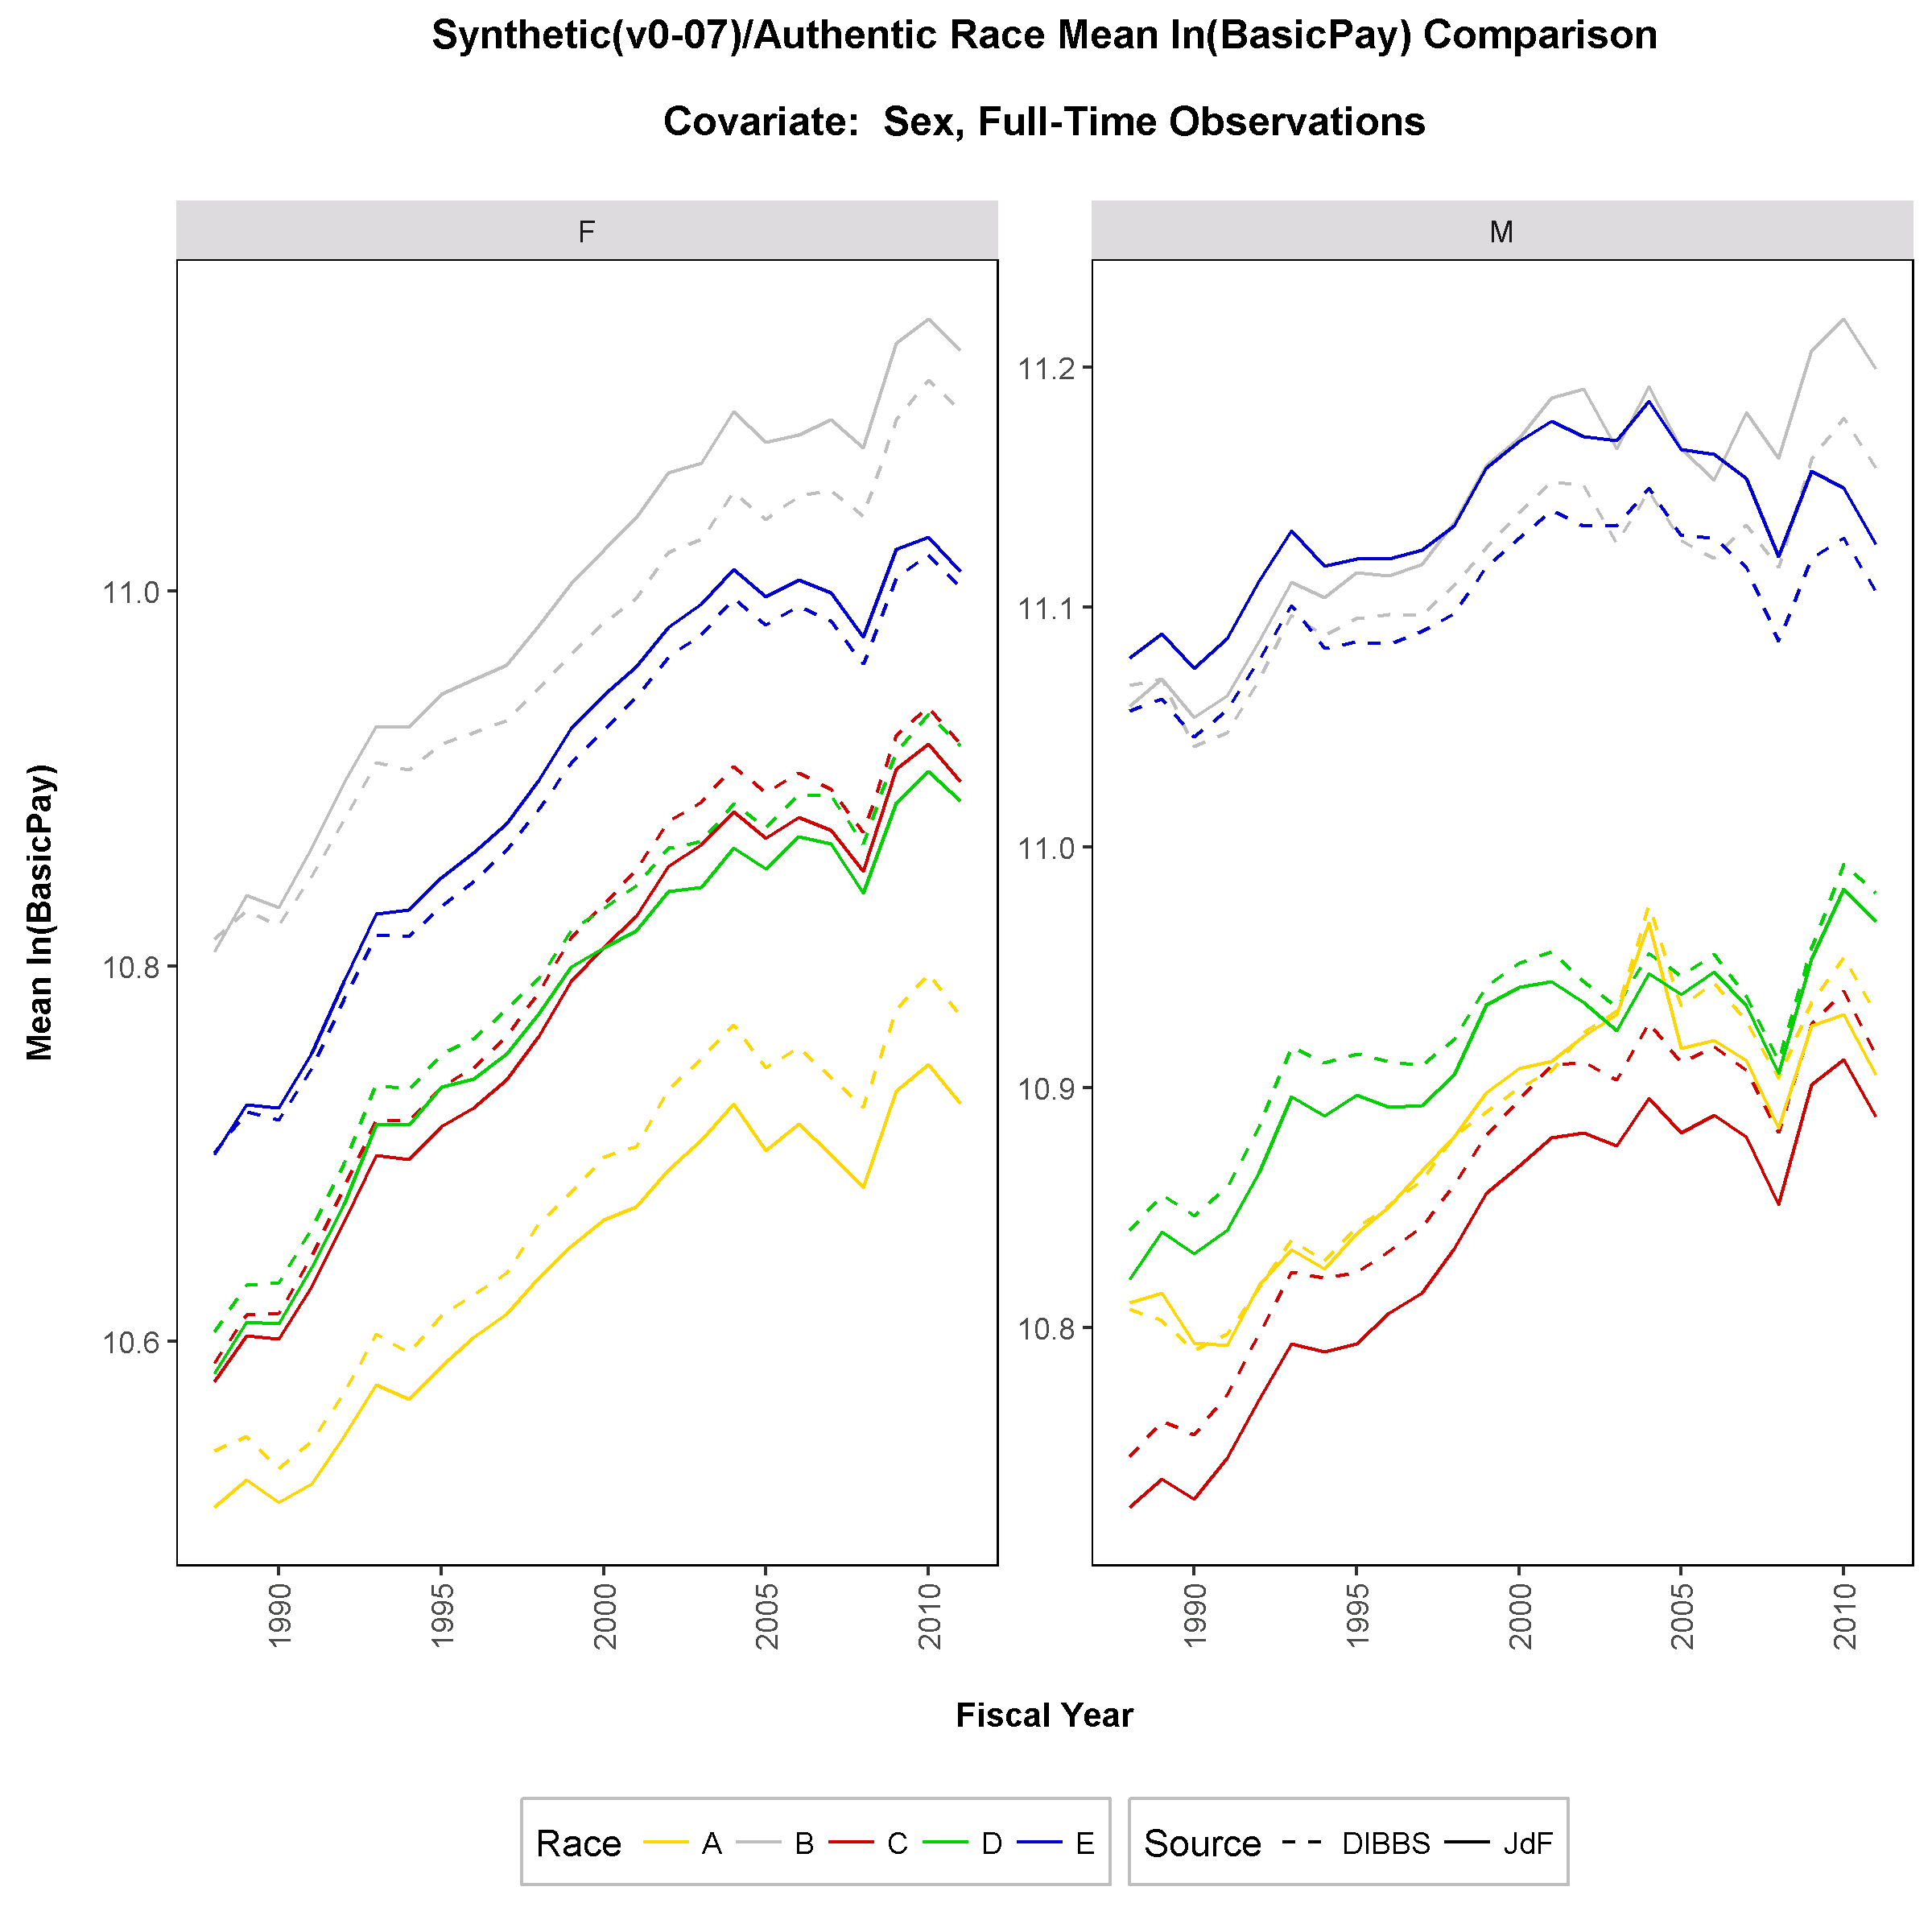
\includegraphics[width=6.5in, trim={0 0 0 0.75in}, clip]{RaceLogPayBySex-FY.png}
    \caption{Mean basic pay by sex, race, and year.  Female on left, male on right.  Race codes:  A = Native American, B = Asian, C = black, D = Hispanic, E = white.  Dashed line for synthetic data, solid line for authentic.}
    \label{figure:RaceLogPayBySex-FY}
\end{figure}

\clearpage

GENDER PAY DIFFERENTIAL FIXED EFFECTS QUANTILE REGRESSION MODEL\\

Figure \ref{figure:GenderPayDifferentialQuantileRegressionAgeRaceEdPanelv0-06} plots the 0.1, 0.5, and 0.9 quantile estimates of difference in log(basic pay) between federal employee women and men by year, controlled for race, age, education, agency, and occupation.\\

Observation:  Although some systematic separation appears between data sets, trends indicate similar proportion change with respect to time.

\vspace{20pt}

\begin{figure}[h!]
    \centering
    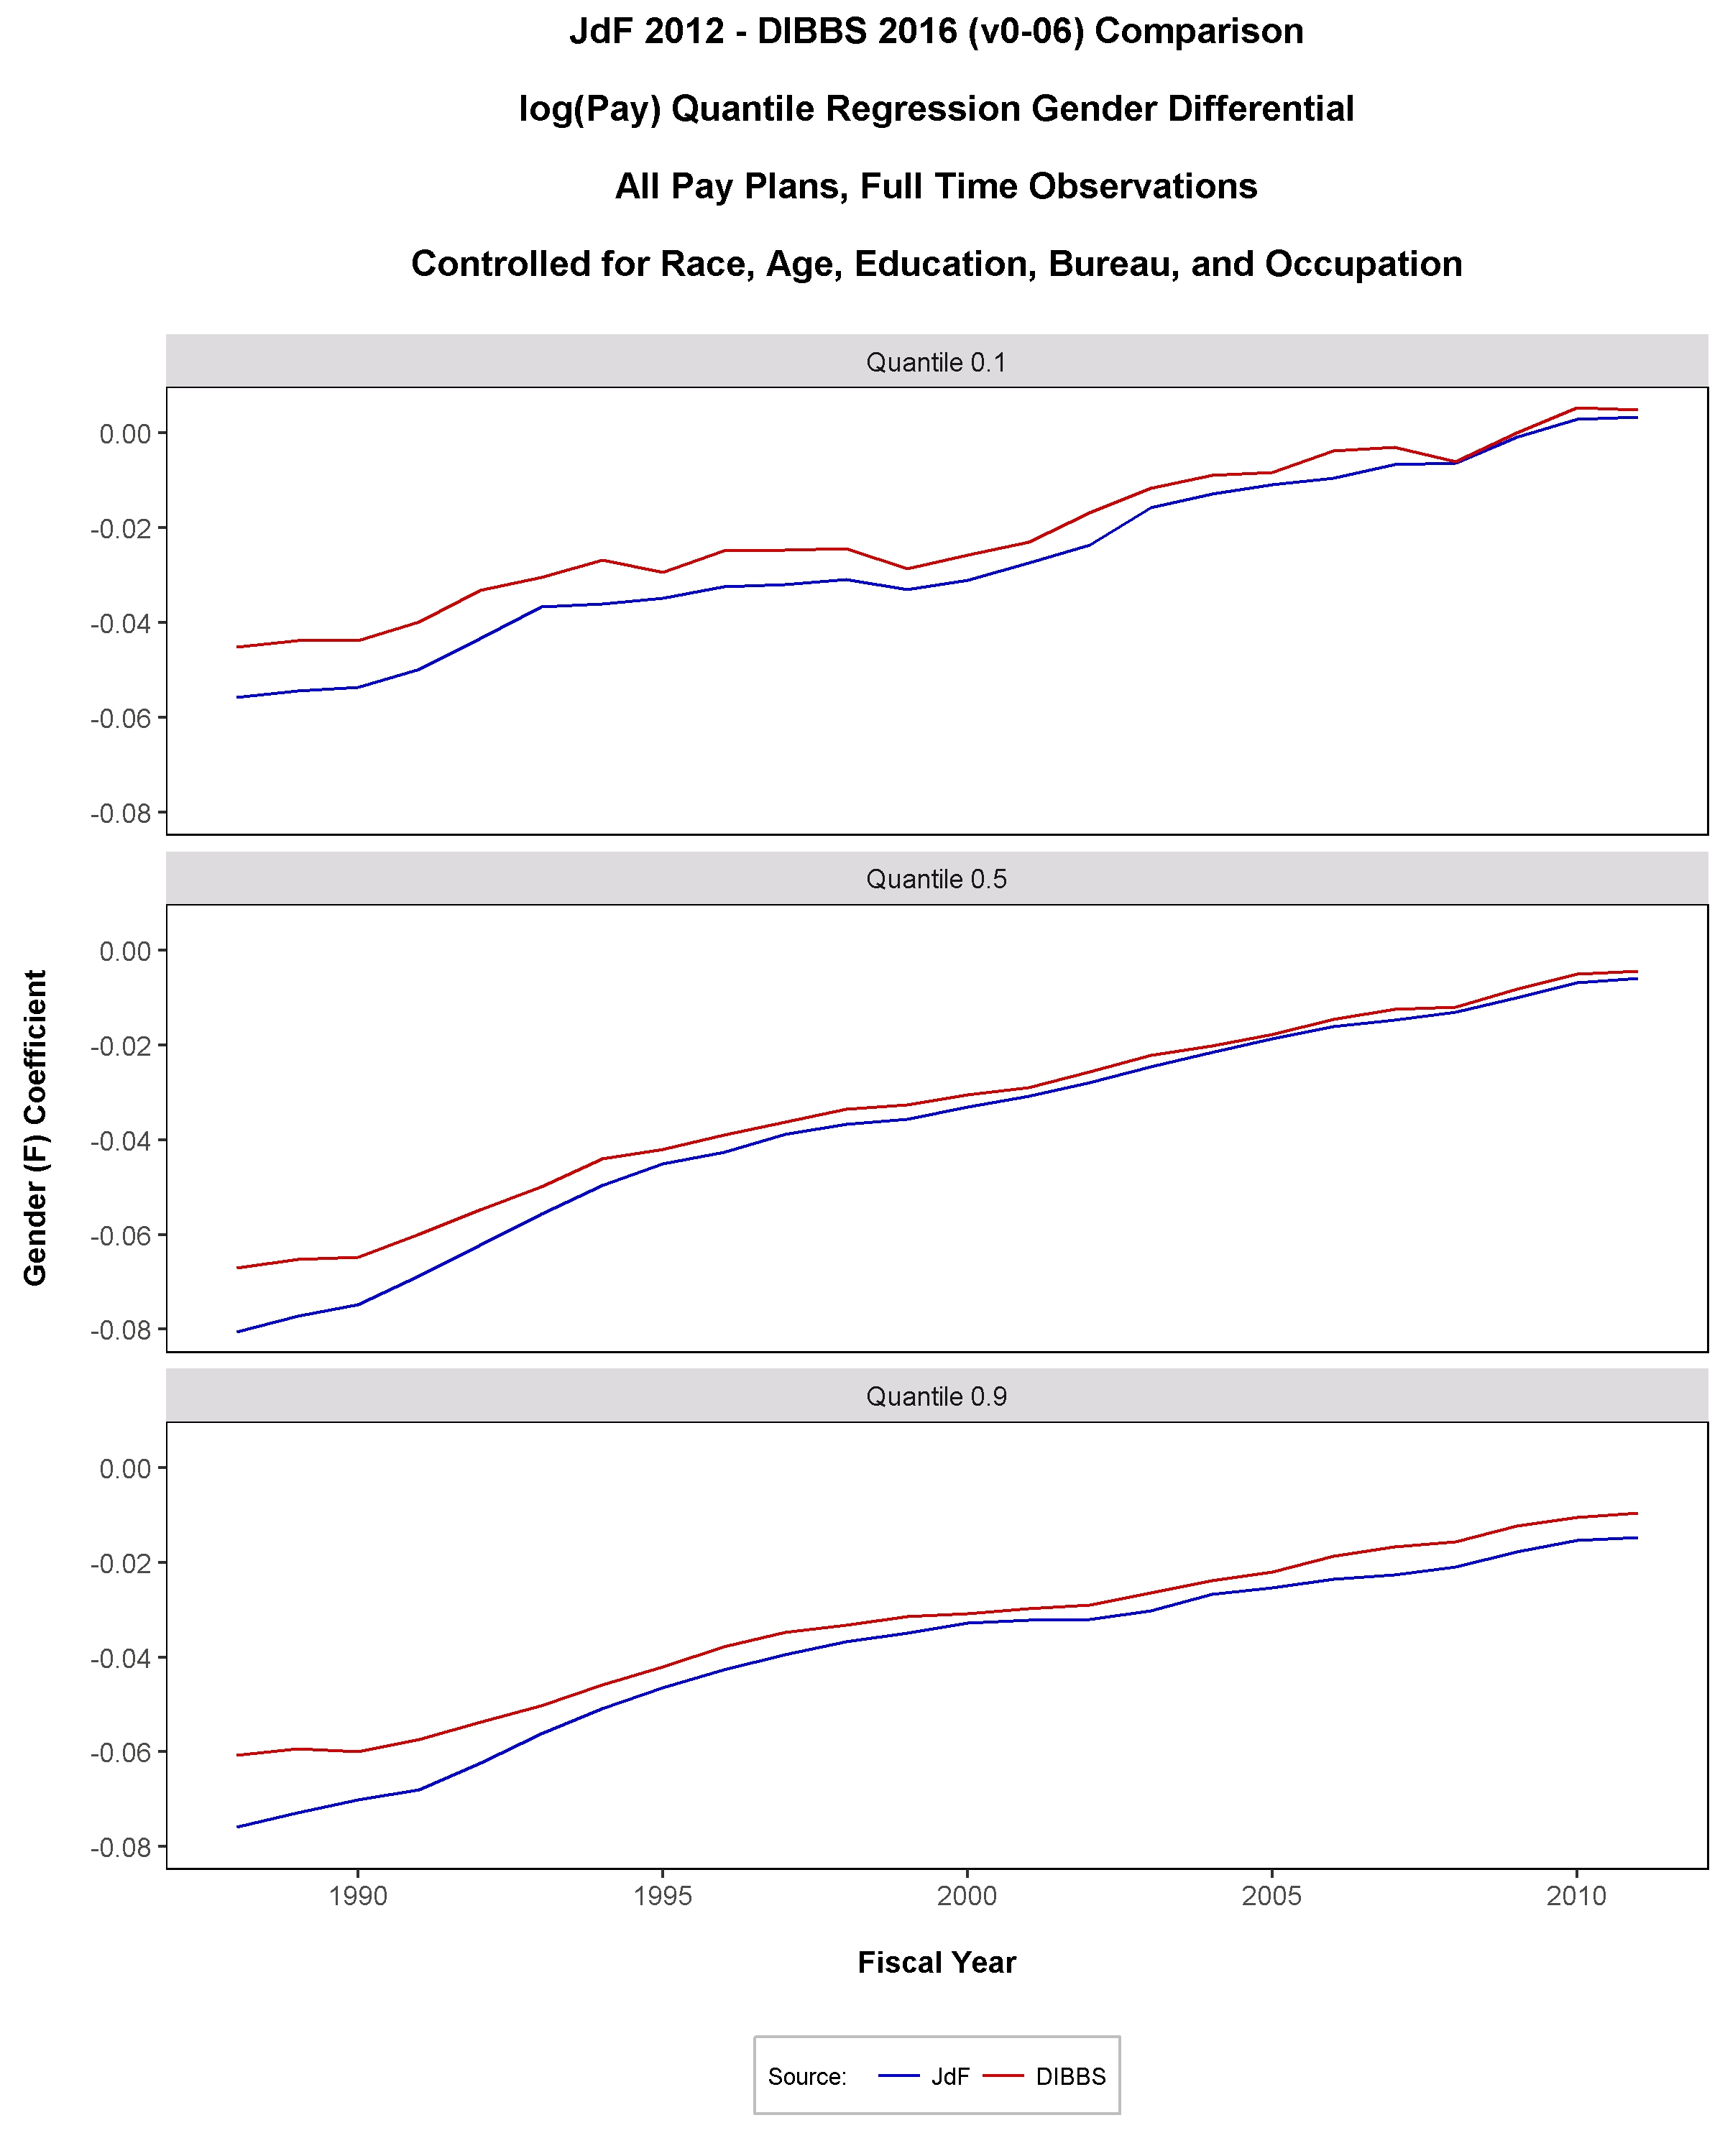
\includegraphics[width=6in, trim={0 0 0 1.5in}, clip]{GenderPayDifferentialQuantileRegressionAgeRaceEdPanelv0-06.png}
    \caption{Quantile estimates from gender pay disparity fixed effects model.  Upper line from synthetic data, lower line from authentic.}
    \label{figure:GenderPayDifferentialQuantileRegressionAgeRaceEdPanelv0-06}
\end{figure}

\clearpage

GENDER PROPORTION BY RACE, EDUCATION, AND YEAR\\

Proportion observations by gender is critical in models involving gender effects.  Figure \ref{figure:GenderProportionLogisticModelEducationRaceFYScaleFixedv0-06} plots proportion female employees by race, education, and year.  Fitted lines are logistic regression models.\\

Observation:  This four-way comparison (sex, race, education, and year) confirms good representation in synthetic data of gender proportion among important variable combinations in the authentic data.  Fitted logistic regression models have nearly identical trends through fiscal years.  Note the slight degradation in fit as observation count (n) decreases.\\

\vspace{20pt}

\begin{figure}[h!]
    \centering
    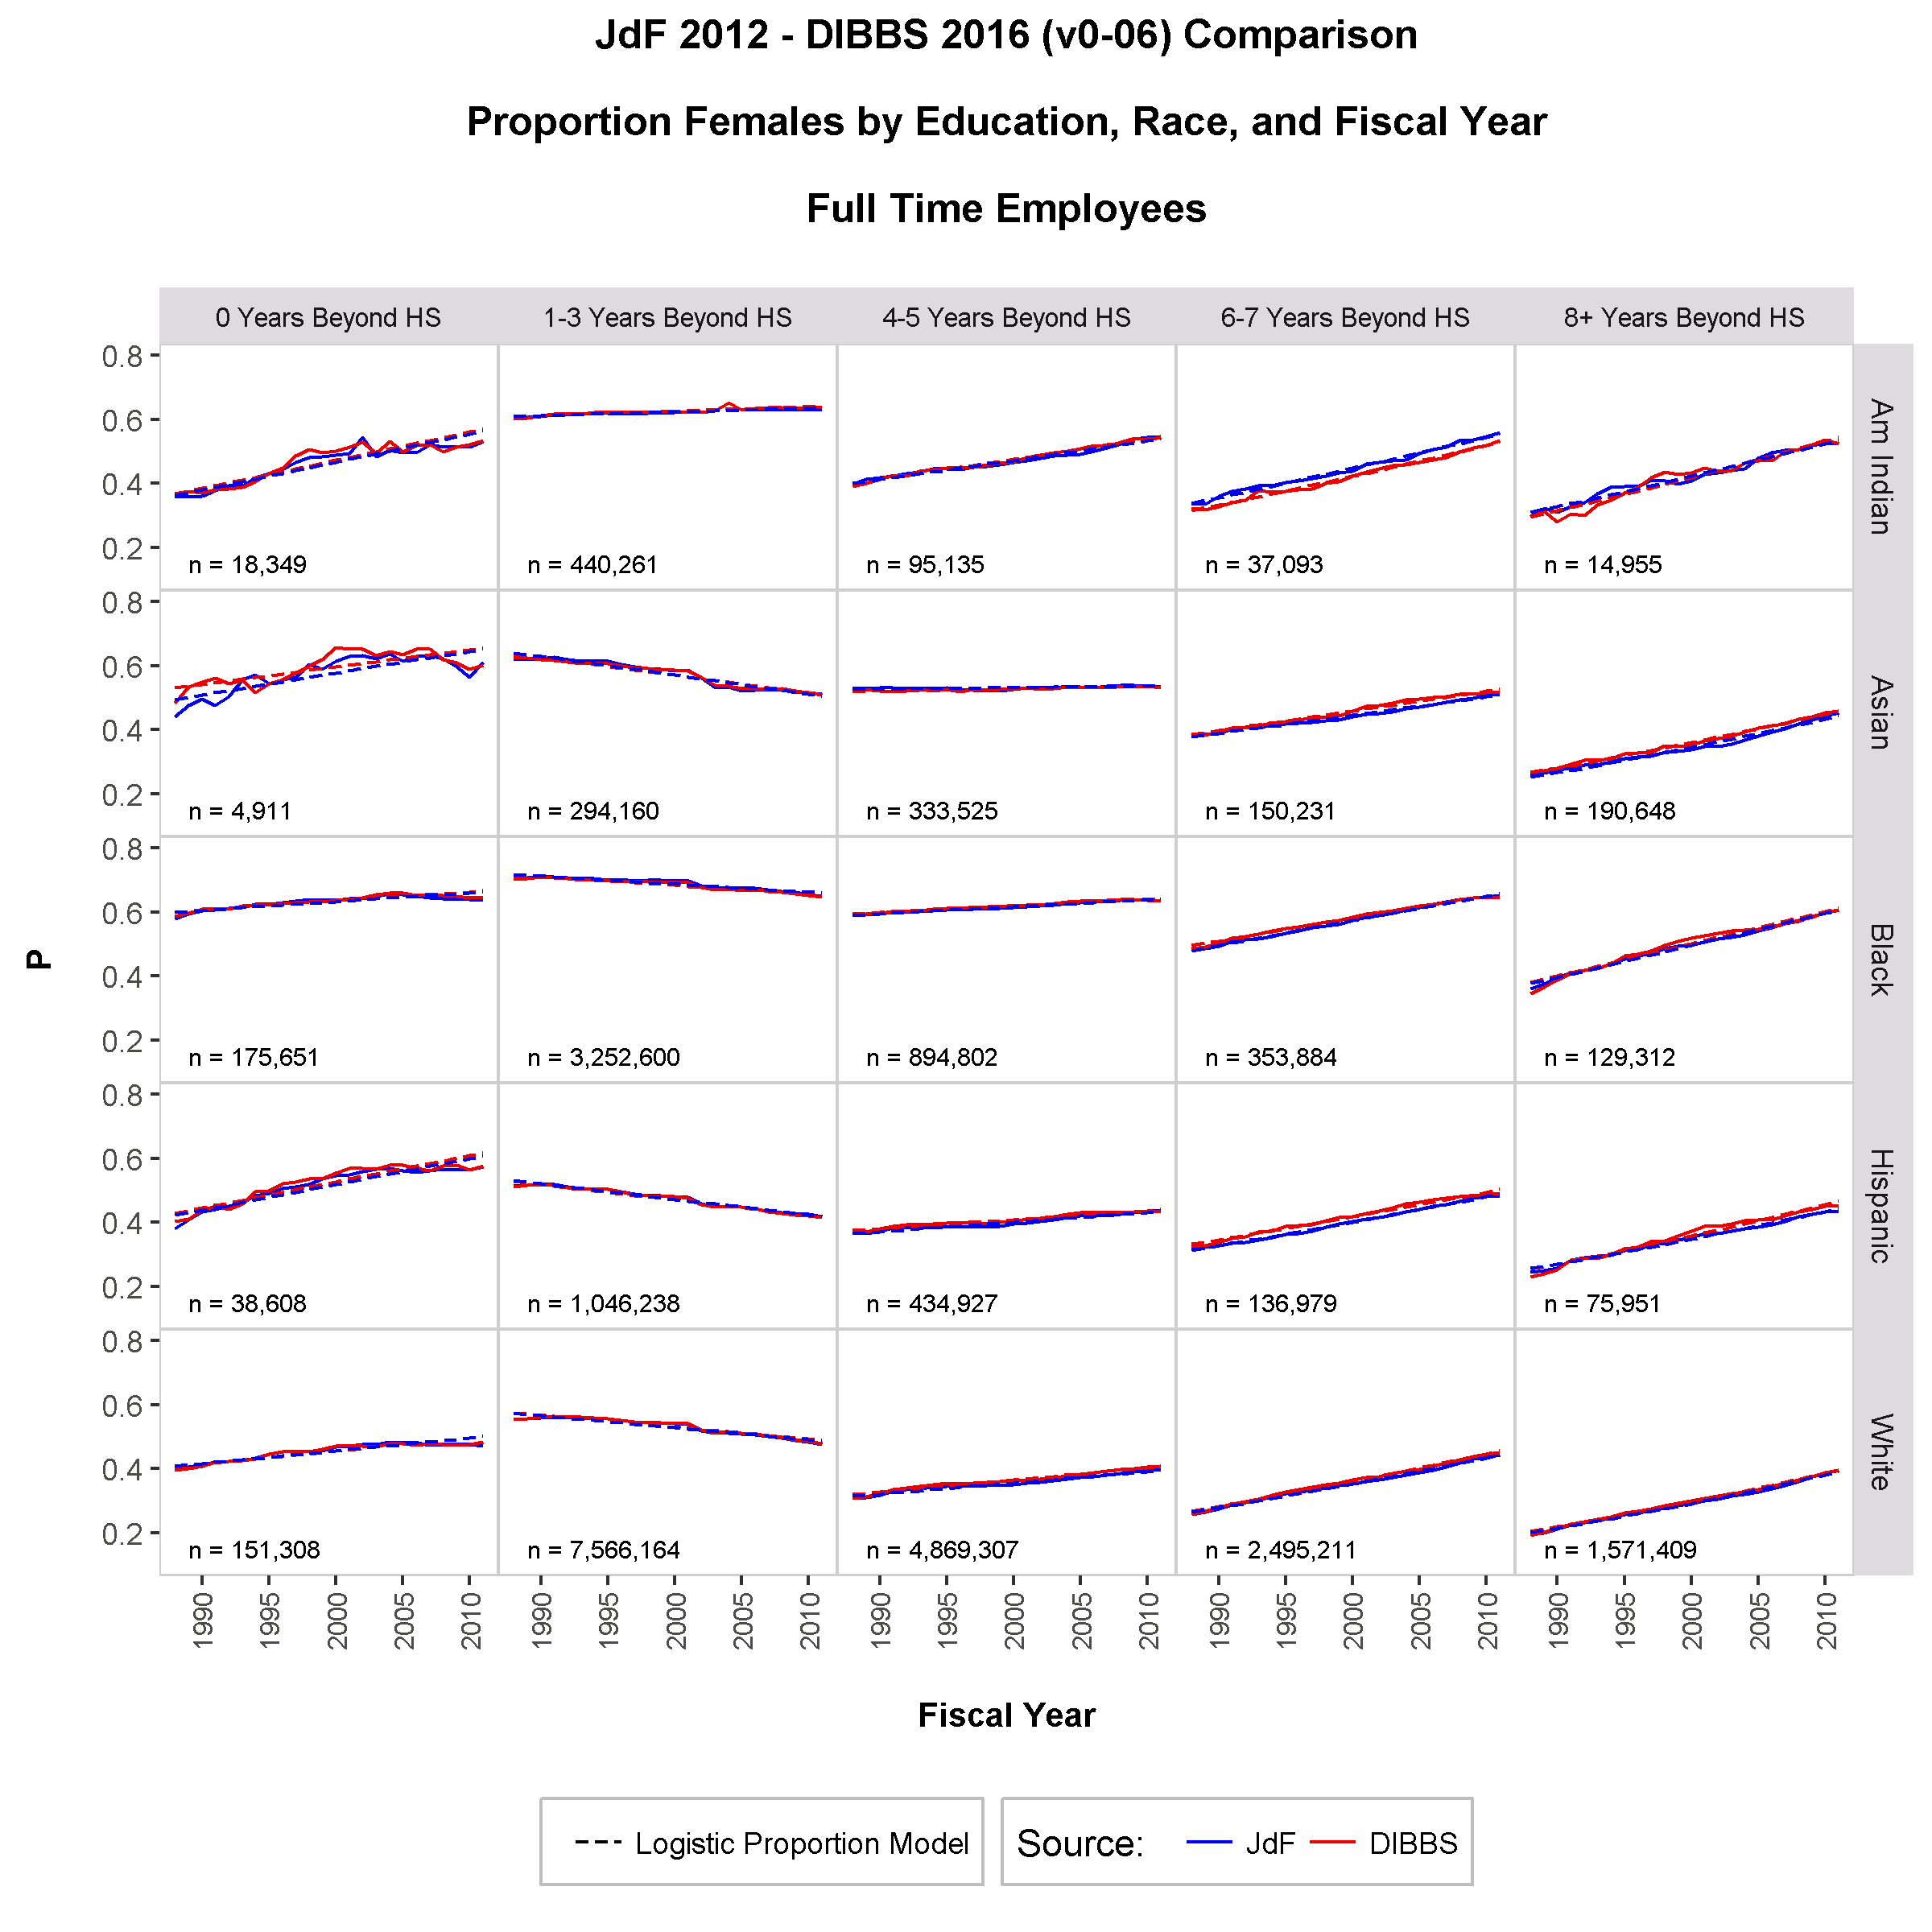
\includegraphics[width=6.5in, trim={0 0 0 1in}, clip]{GenderProportionLogisticModelEducationRaceFYScaleFixedv0-06.png}
    \caption{Proportion female observations by race, education, and year.  Fitted lines are logistic regression estimates.}
    \label{figure:GenderProportionLogisticModelEducationRaceFYScaleFixedv0-06}
\end{figure}

\clearpage

GENDER PROPORTION BY RACE, AGE, AND YEAR\\

Figures \ref{figure:GenderProportionLogisticModelFYRaceAgeA} through \ref{figure:GenderProportionLogisticModelFYRaceAgeE}, show for each race, proportion female employees by age and year.  Fitted lines are logistic regression models.\\

Observation:  These four-way comparisons (sex, race, age, and year) confirm good representation in synthetic data of gender proportion among important variable combinations in the authentic data.  Fitted logistic regression models have nearly identical trends through fiscal years.\\

Logistic models reveal agreement in trends between data sets.

\vspace{20pt}

\begin{figure}[h!]
    \centering
    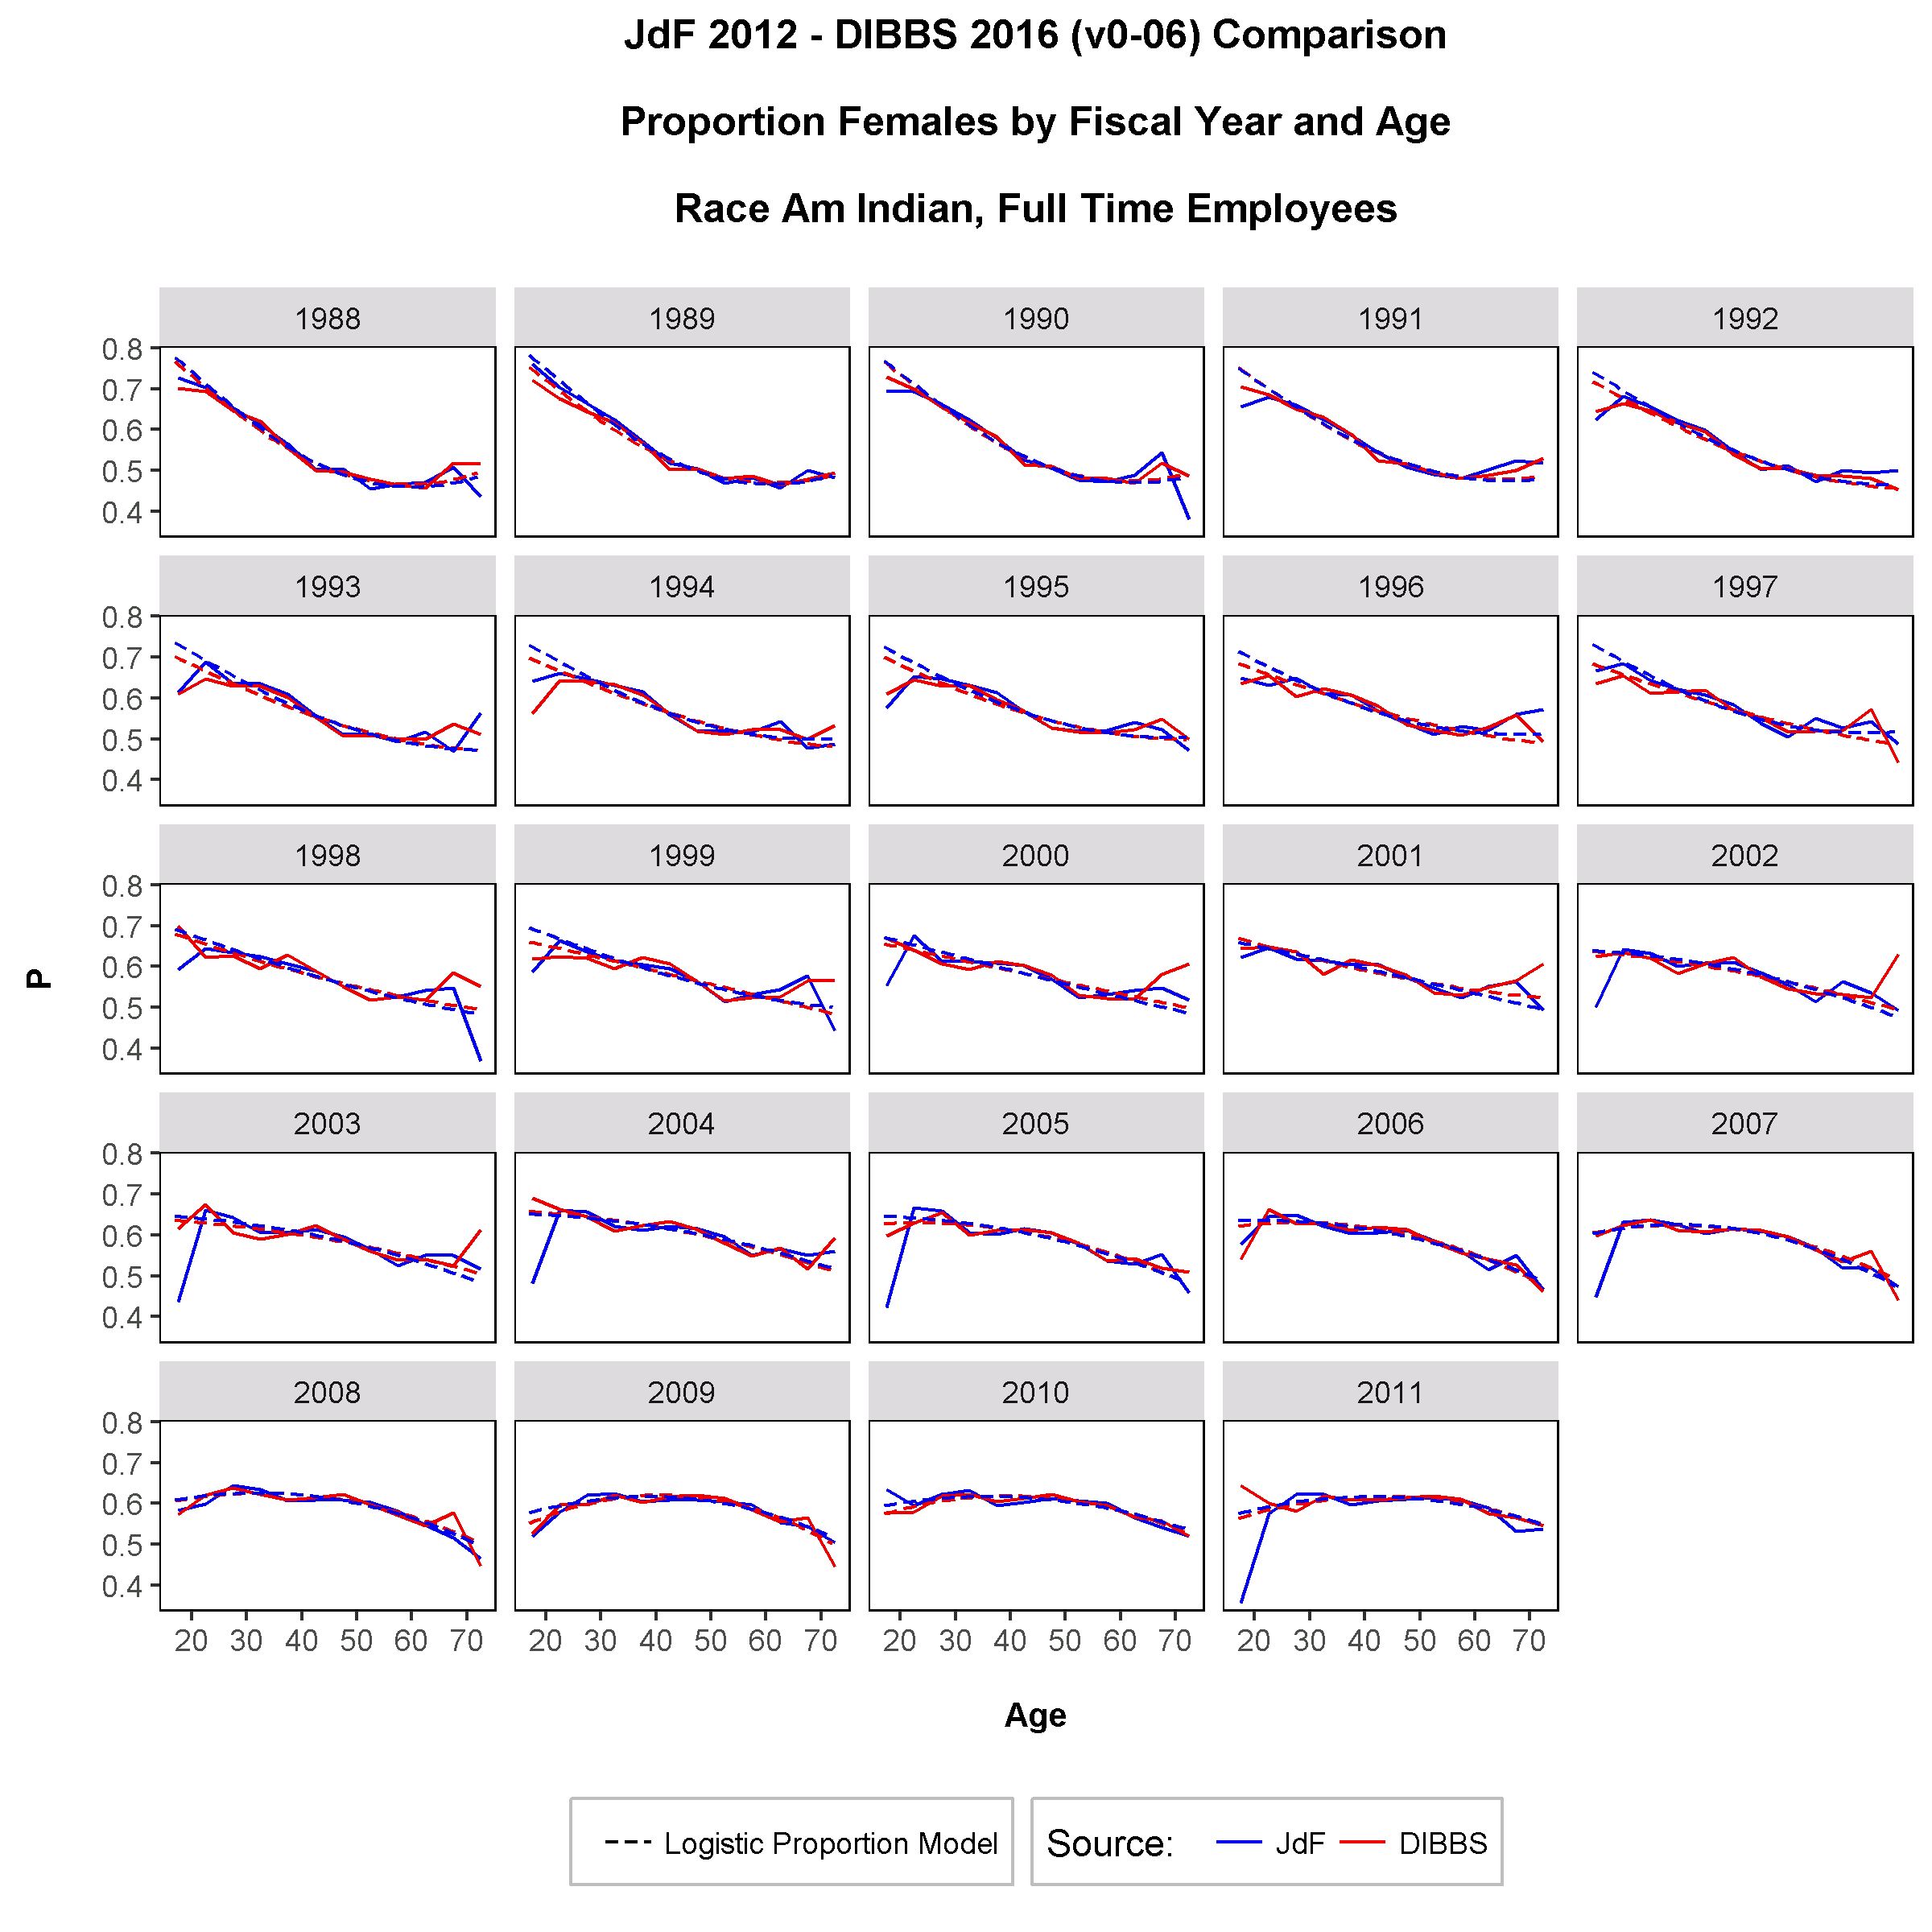
\includegraphics[width=6.5in, trim={0 0 0 1in}, clip]{GenderProportionLogisticModelFYRaceAgeAv0-06.png}
    \caption{Proportion female observations by education and year.  Race Native American.  Fitted lines are logistic regression estimates.}
    \label{figure:GenderProportionLogisticModelFYRaceAgeA}
\end{figure}

\clearpage

\begin{figure}[h]
    \centering
    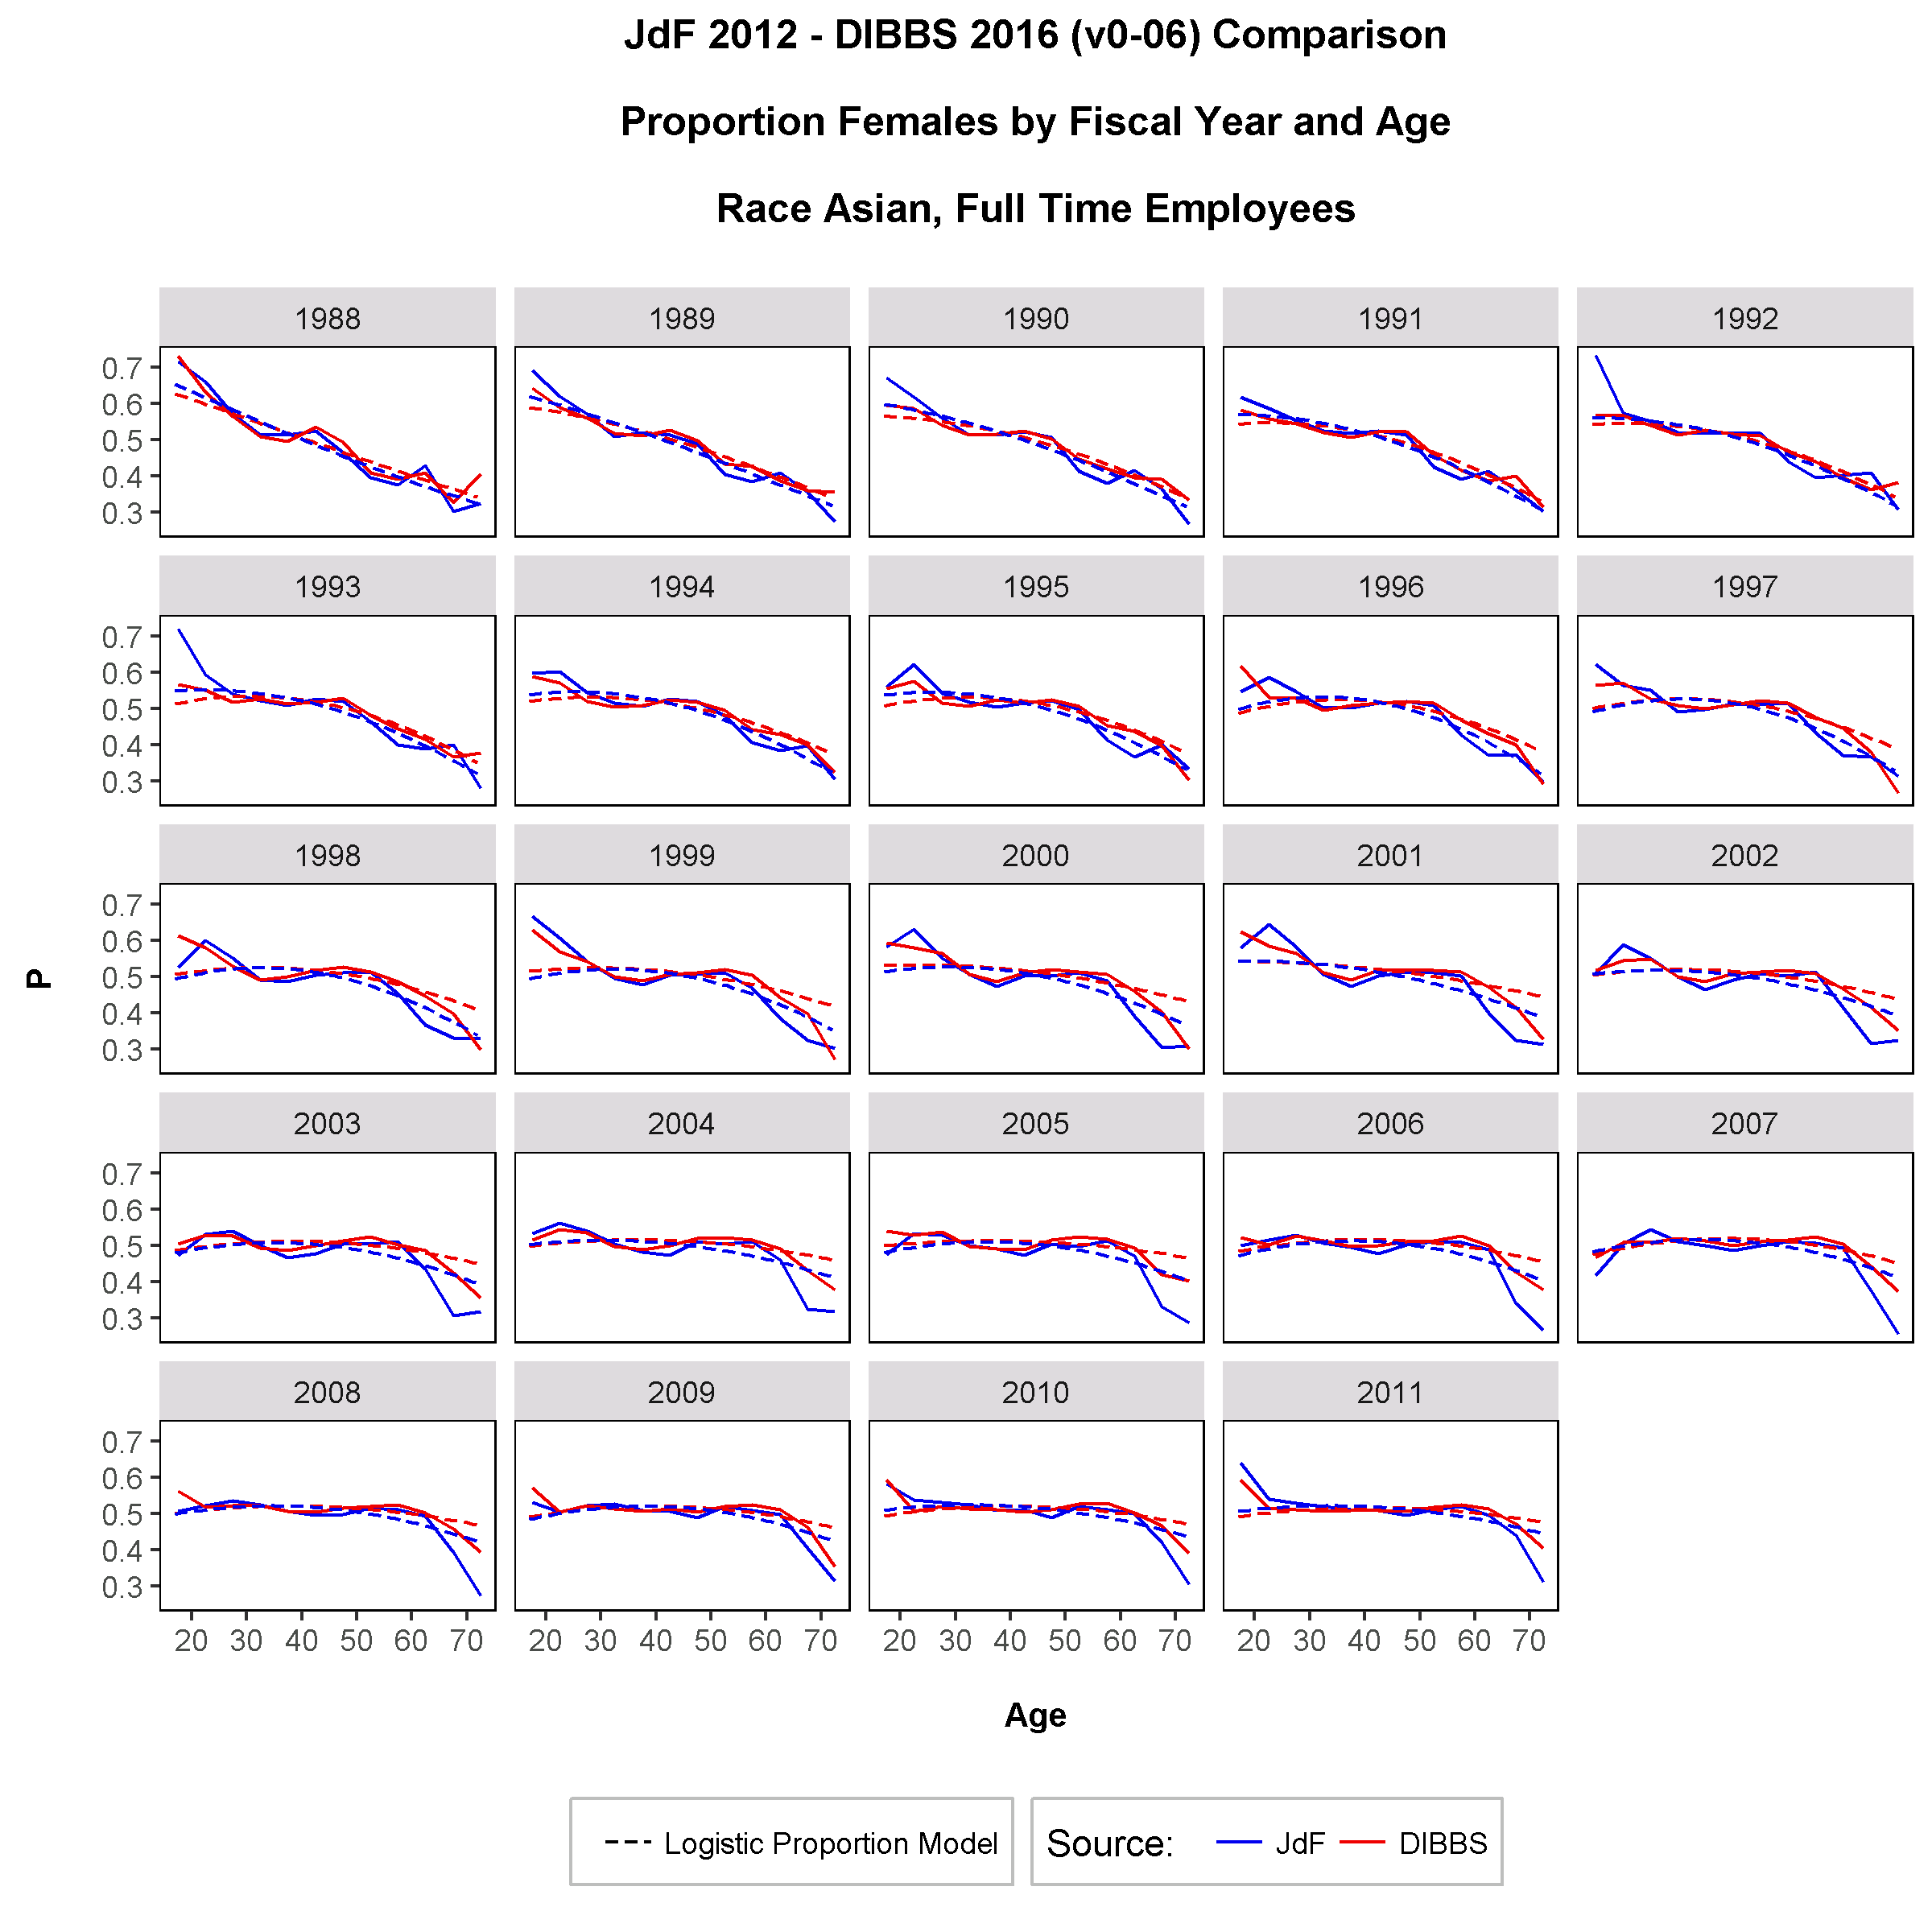
\includegraphics[width=6.5in, trim={0 0 0 1in}, clip]{GenderProportionLogisticModelFYRaceAgeBv0-06.png}
    \caption{Proportion female observations by education and year.  Race Asian.  Fitted lines are logistic regression estimates.}
    \label{figure:GenderProportionLogisticModelFYRaceAgeB}
\end{figure}

\clearpage

\begin{figure}[h]
    \centering
    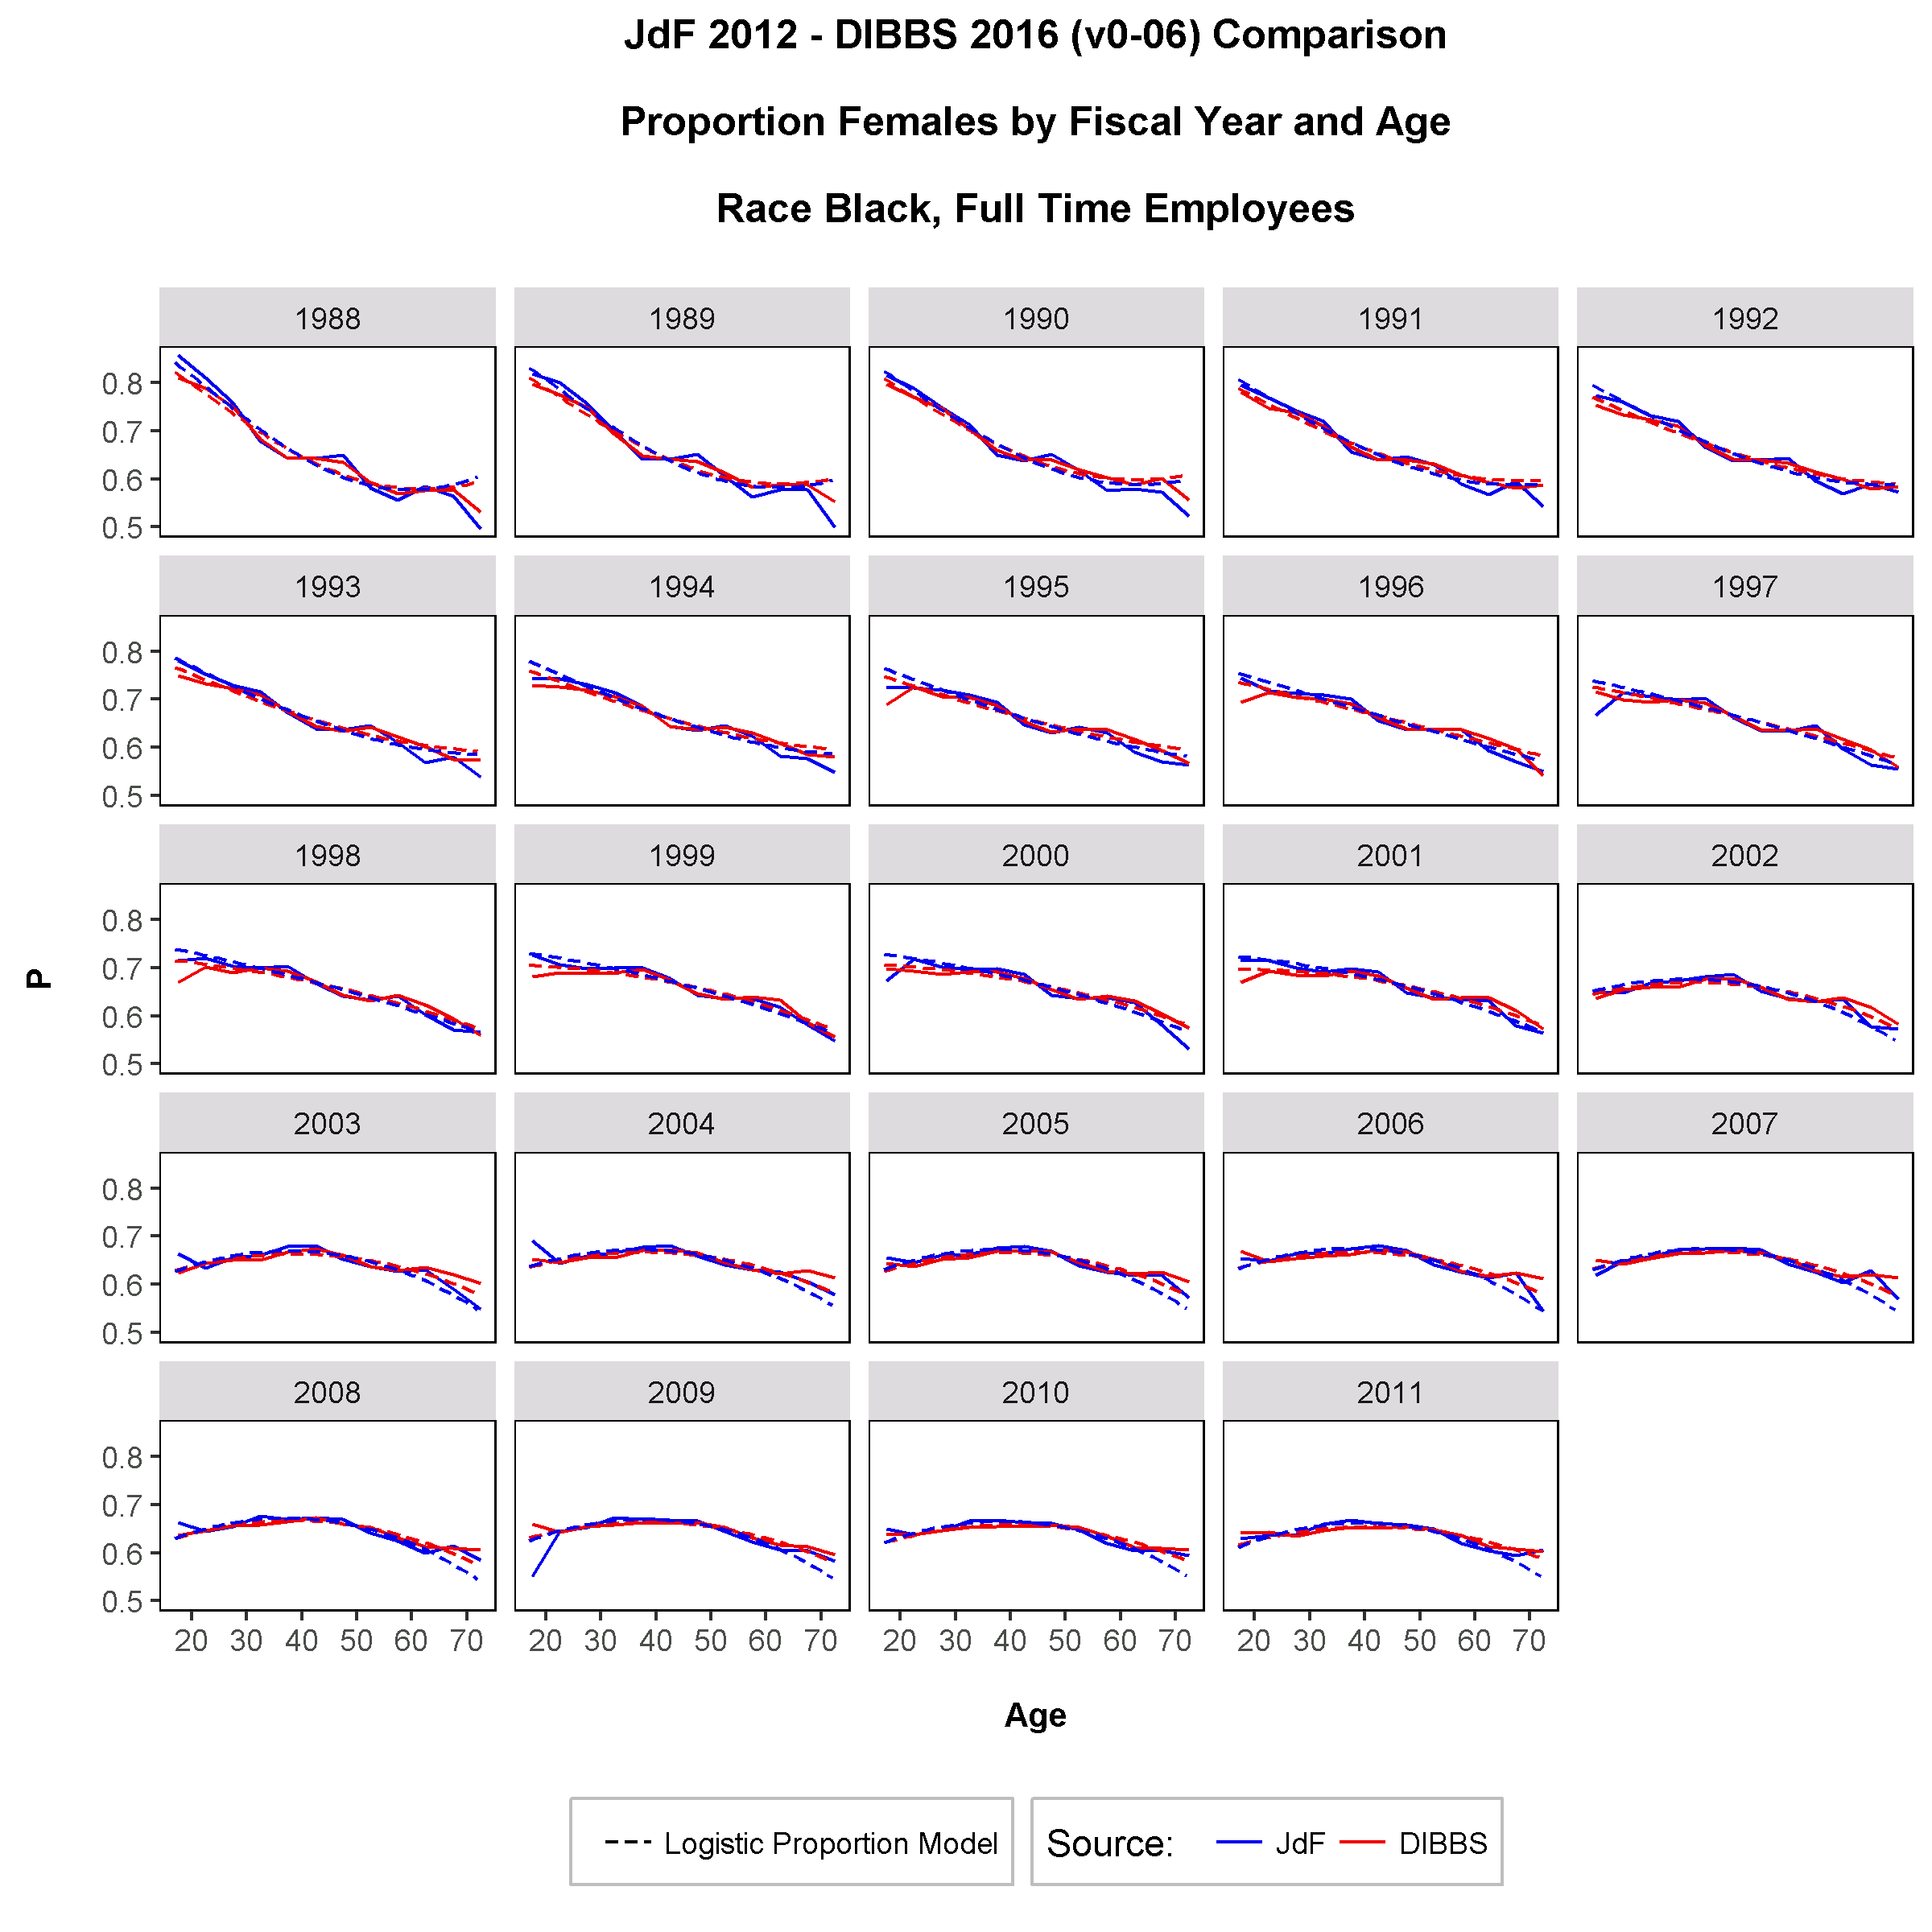
\includegraphics[width=6.5in, trim={0 0 0 1in}, clip]{GenderProportionLogisticModelFYRaceAgeCv0-06.png}
    \caption{Proportion female observations by education and year.  Race black.  Fitted lines are logistic regression estimates.}
    \label{figure:GenderProportionLogisticModelFYRaceAgeC}
\end{figure}

\clearpage

\begin{figure}[h]
    \centering
    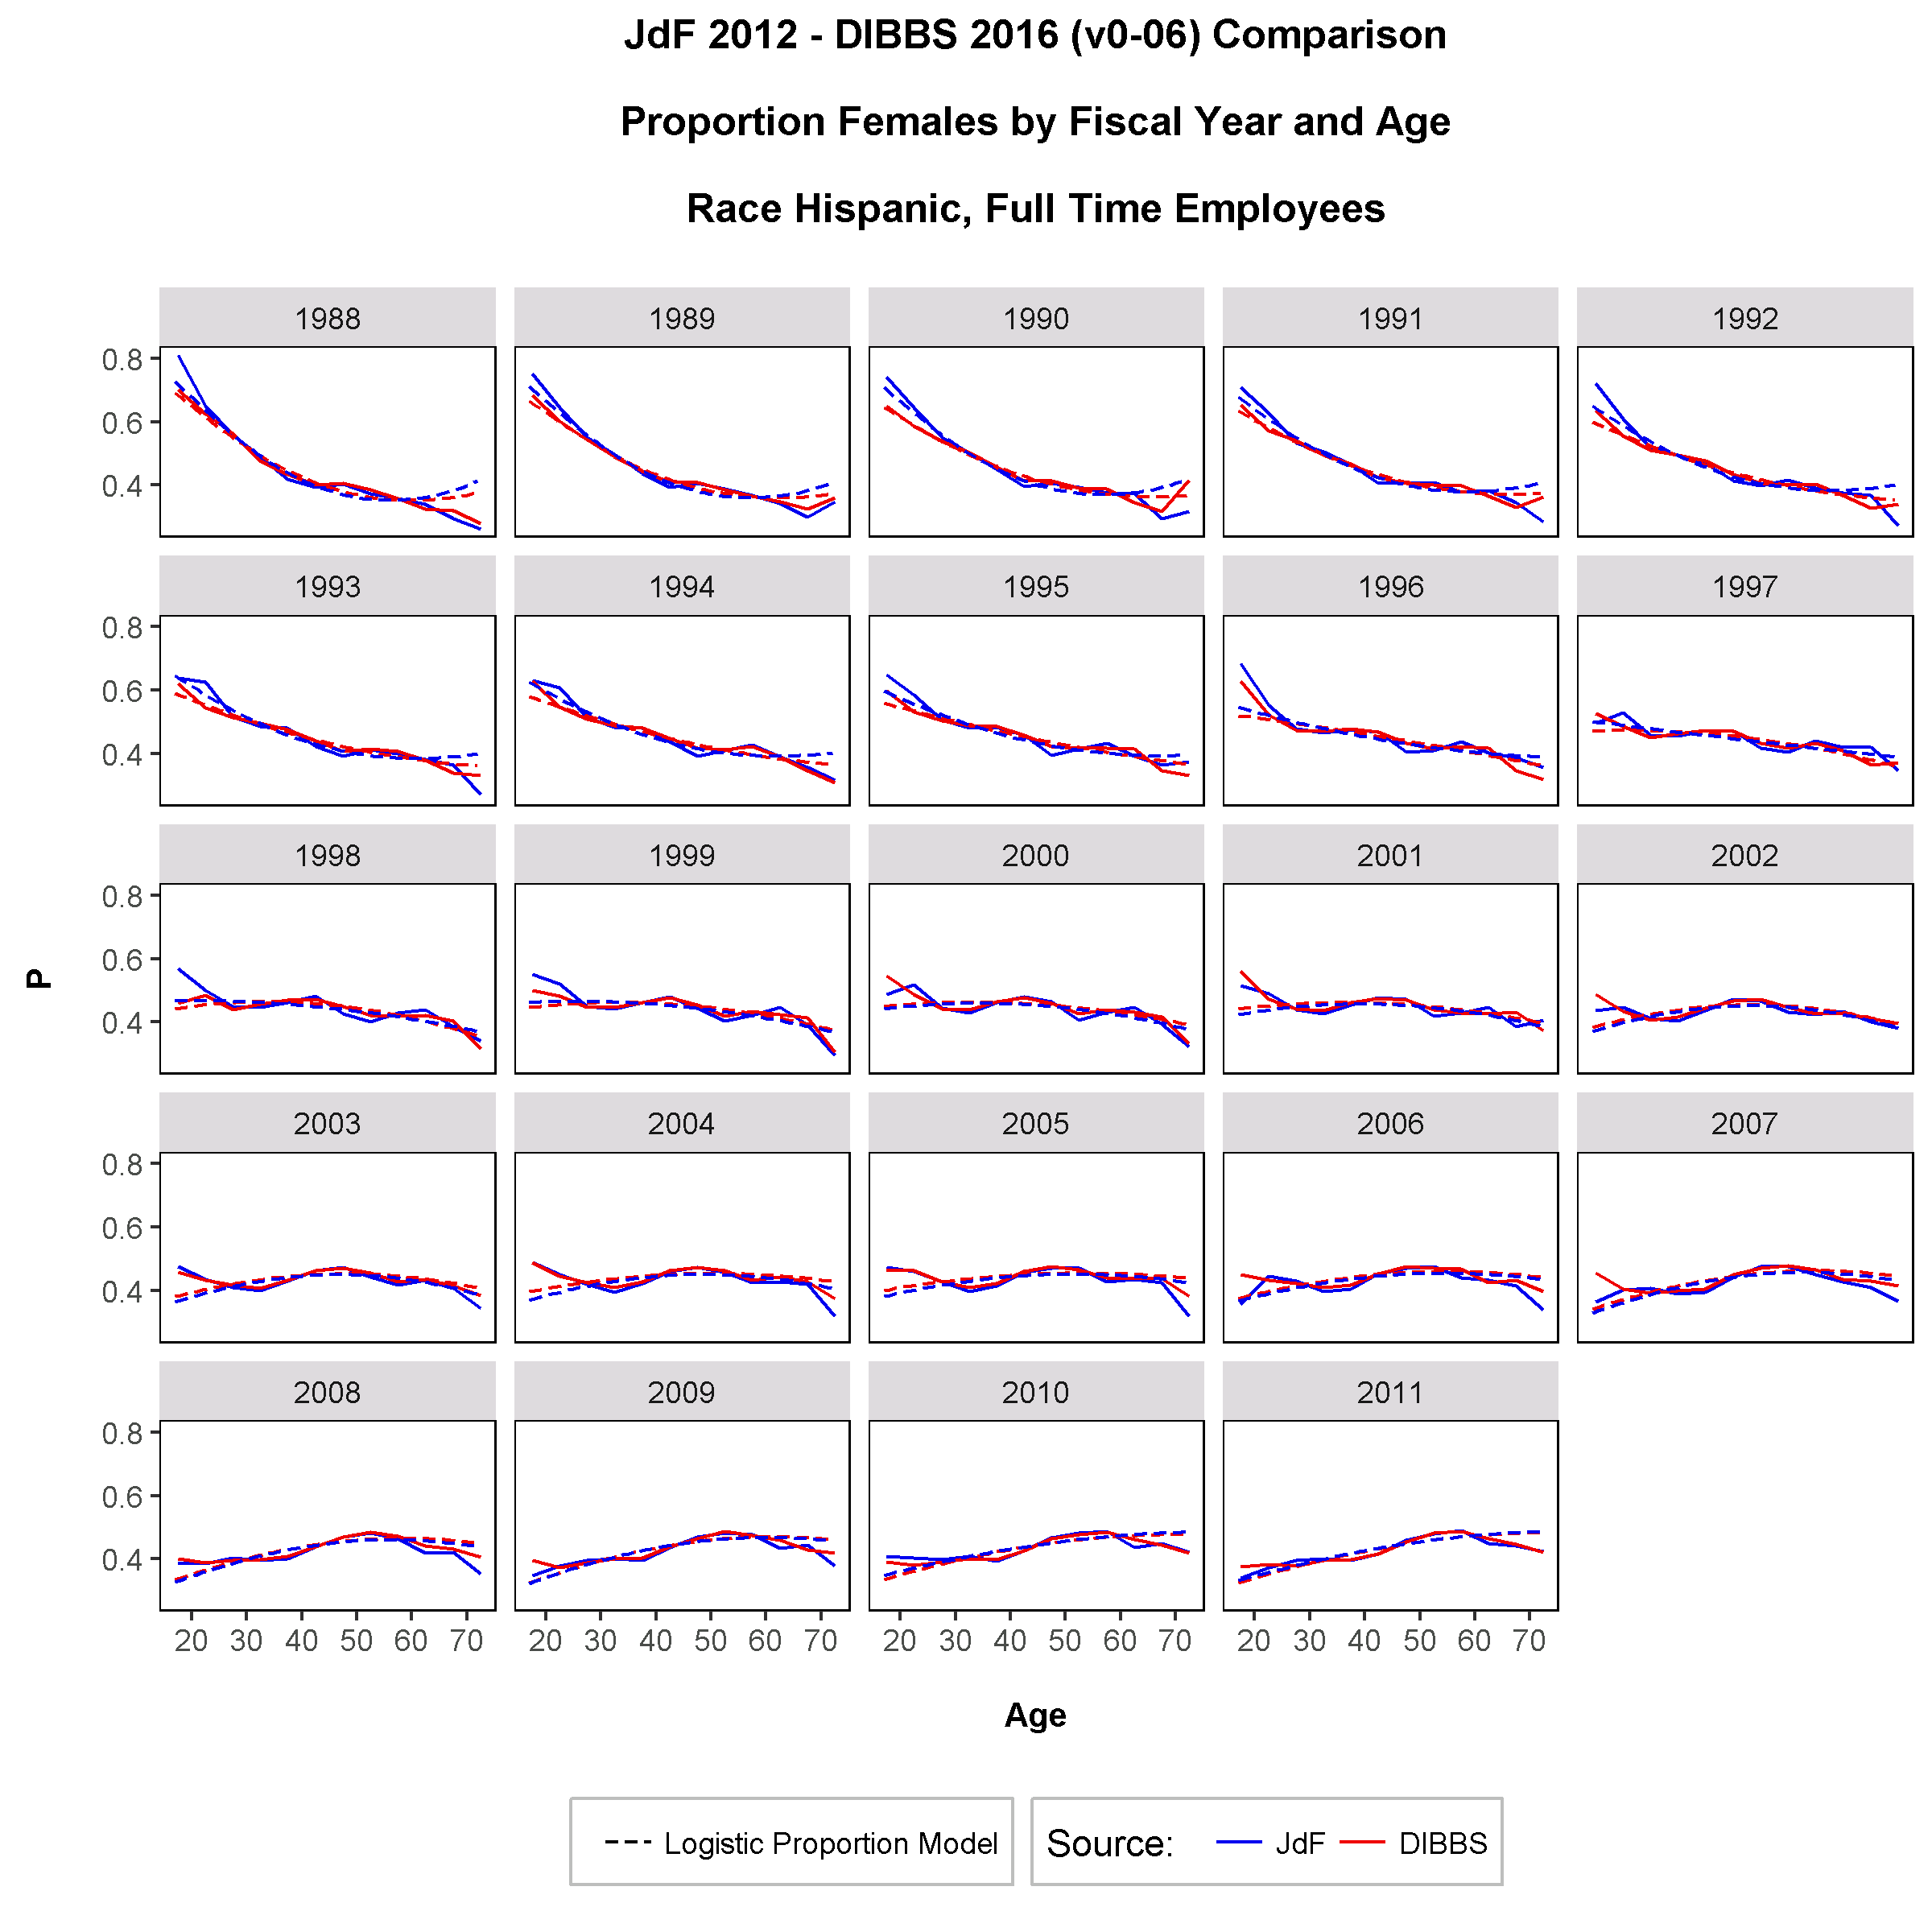
\includegraphics[width=6.5in, trim={0 0 0 1in}, clip]{GenderProportionLogisticModelFYRaceAgeDv0-06.png}
    \caption{Proportion female observations by education and year.  Race Hispanic.  Fitted lines are logistic regression estimates.}
    \label{figure:GenderProportionLogisticModelFYRaceAgeD}
\end{figure}

\clearpage

\begin{figure}[h]
\centering
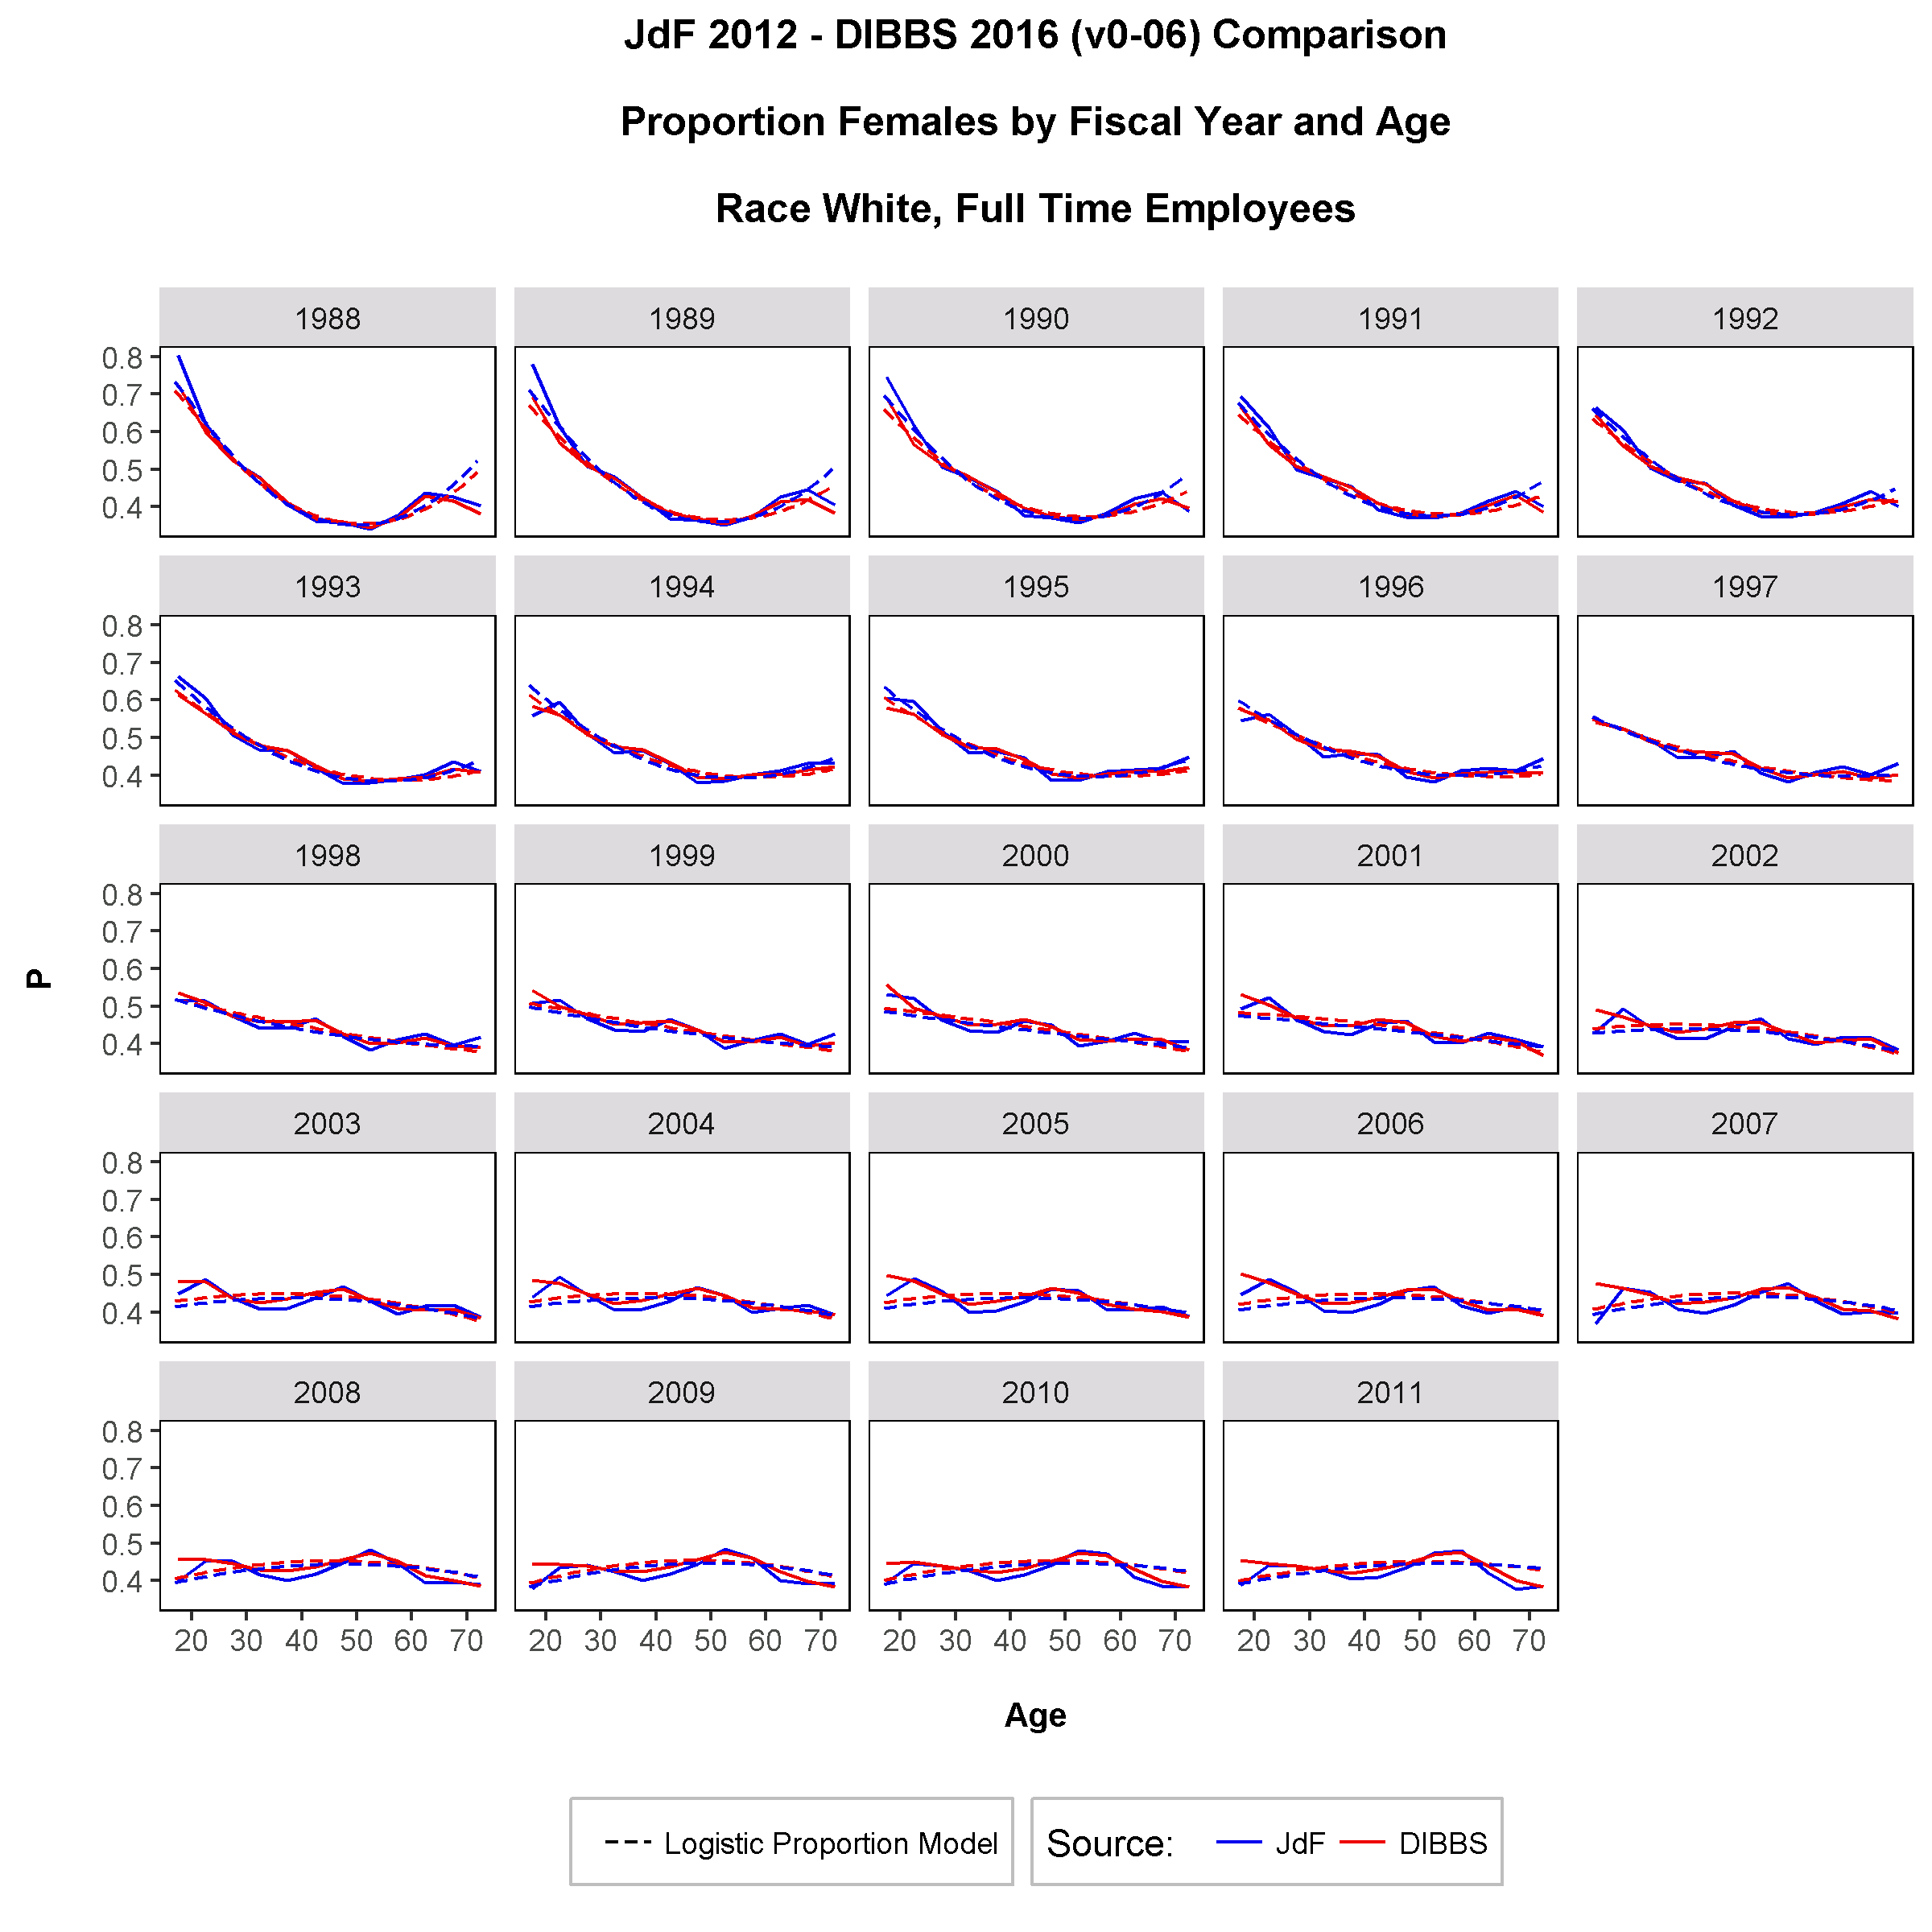
\includegraphics[width=6.5in, trim={0 0 0 1in}, clip]{GenderProportionLogisticModelFYRaceAgeEv0-06.png}
\caption{Proportion female observations by education and year.  Race white.  Fitted lines are logistic regression estimates.}
\label{figure:GenderProportionLogisticModelFYRaceAgeE}
\end{figure}

\clearpage

GENDER PROPORTION BY OCCUPATION\\

In the data supplied by OPM, 205 occupations (more than 25\%) have proportion female observations below 0.05.  12 have proportion female observations greater than 0.95.  Of these occupations, 148 have fewer than 1,000 total observations and 30 haver fewer than 10 observations.  This presents challenges for accurate representation of authentic proportions in synthetic observations, while reducing the risk of individual employee identification.  Figures \ref{figure:JdFDIBBSOccupationProportionBar1} and \ref{figure:JdFDIBBSOccupationProportionBar2} compare proportion female for the first 120 occupation codes.  Figures \ref{figure:JdFDIBBSOccupationProportionBar3} and \ref{figure:JdFDIBBSOccupationProportionBar4} compare proportions for the first 120 trade occupations, which begin at code 2500.  ``n-DIBBS" indicates synthetic observation count, ``n-JdF" indicates corresponding authentic observation count.\\

Observation:  Agreement for large count occupations is indicated by proximity of points.  Departure increases with decrease in observation count.  Trade occupations, having generally low observation count and low proportion female in the authentic data, exhibit greater discrepancies than those observed in non-trade occupations. 

\begin{figure}[h]
    \centering
    \begin{subfigure}{1\textwidth}
        \centering
        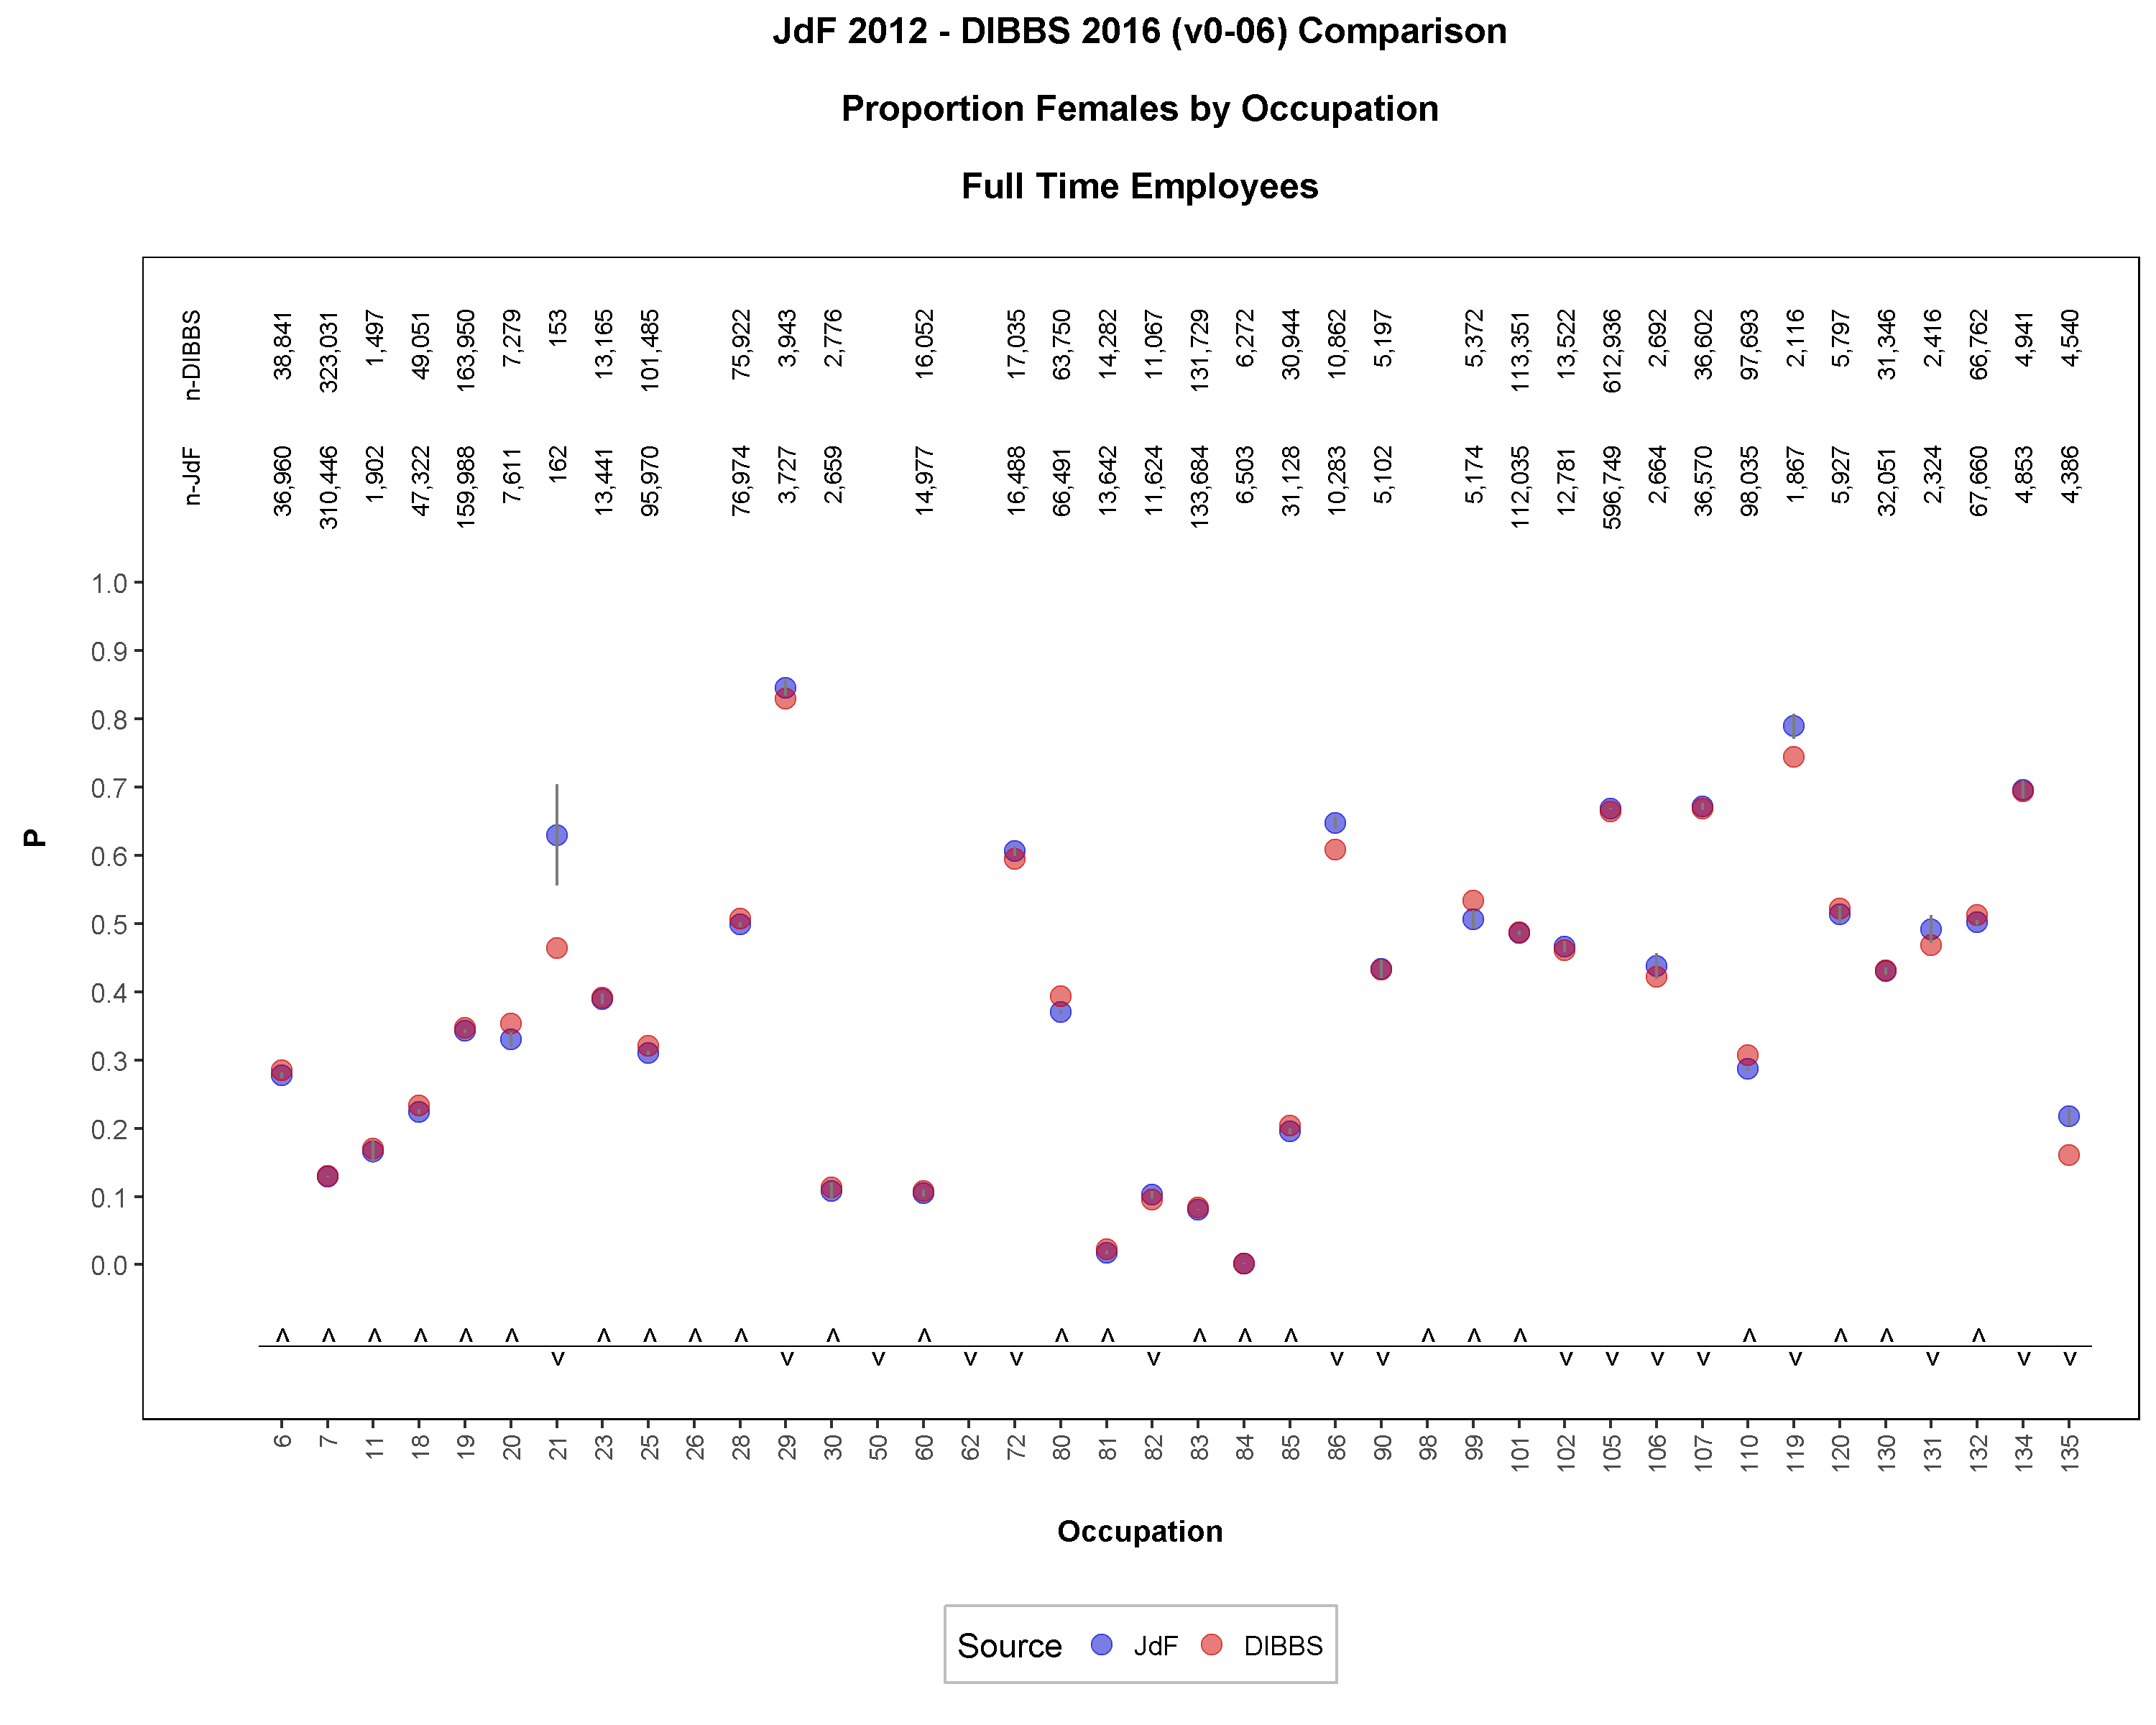
\includegraphics[width=6in, trim={0 1in 0 1in}, clip]{JdFDIBBSOccupationProportionBar1.png}
        \caption{Occupations 0006 through 0135}
        \vspace{10pt}
    \end{subfigure}
    \begin{subfigure}{1\textwidth}
        \centering
        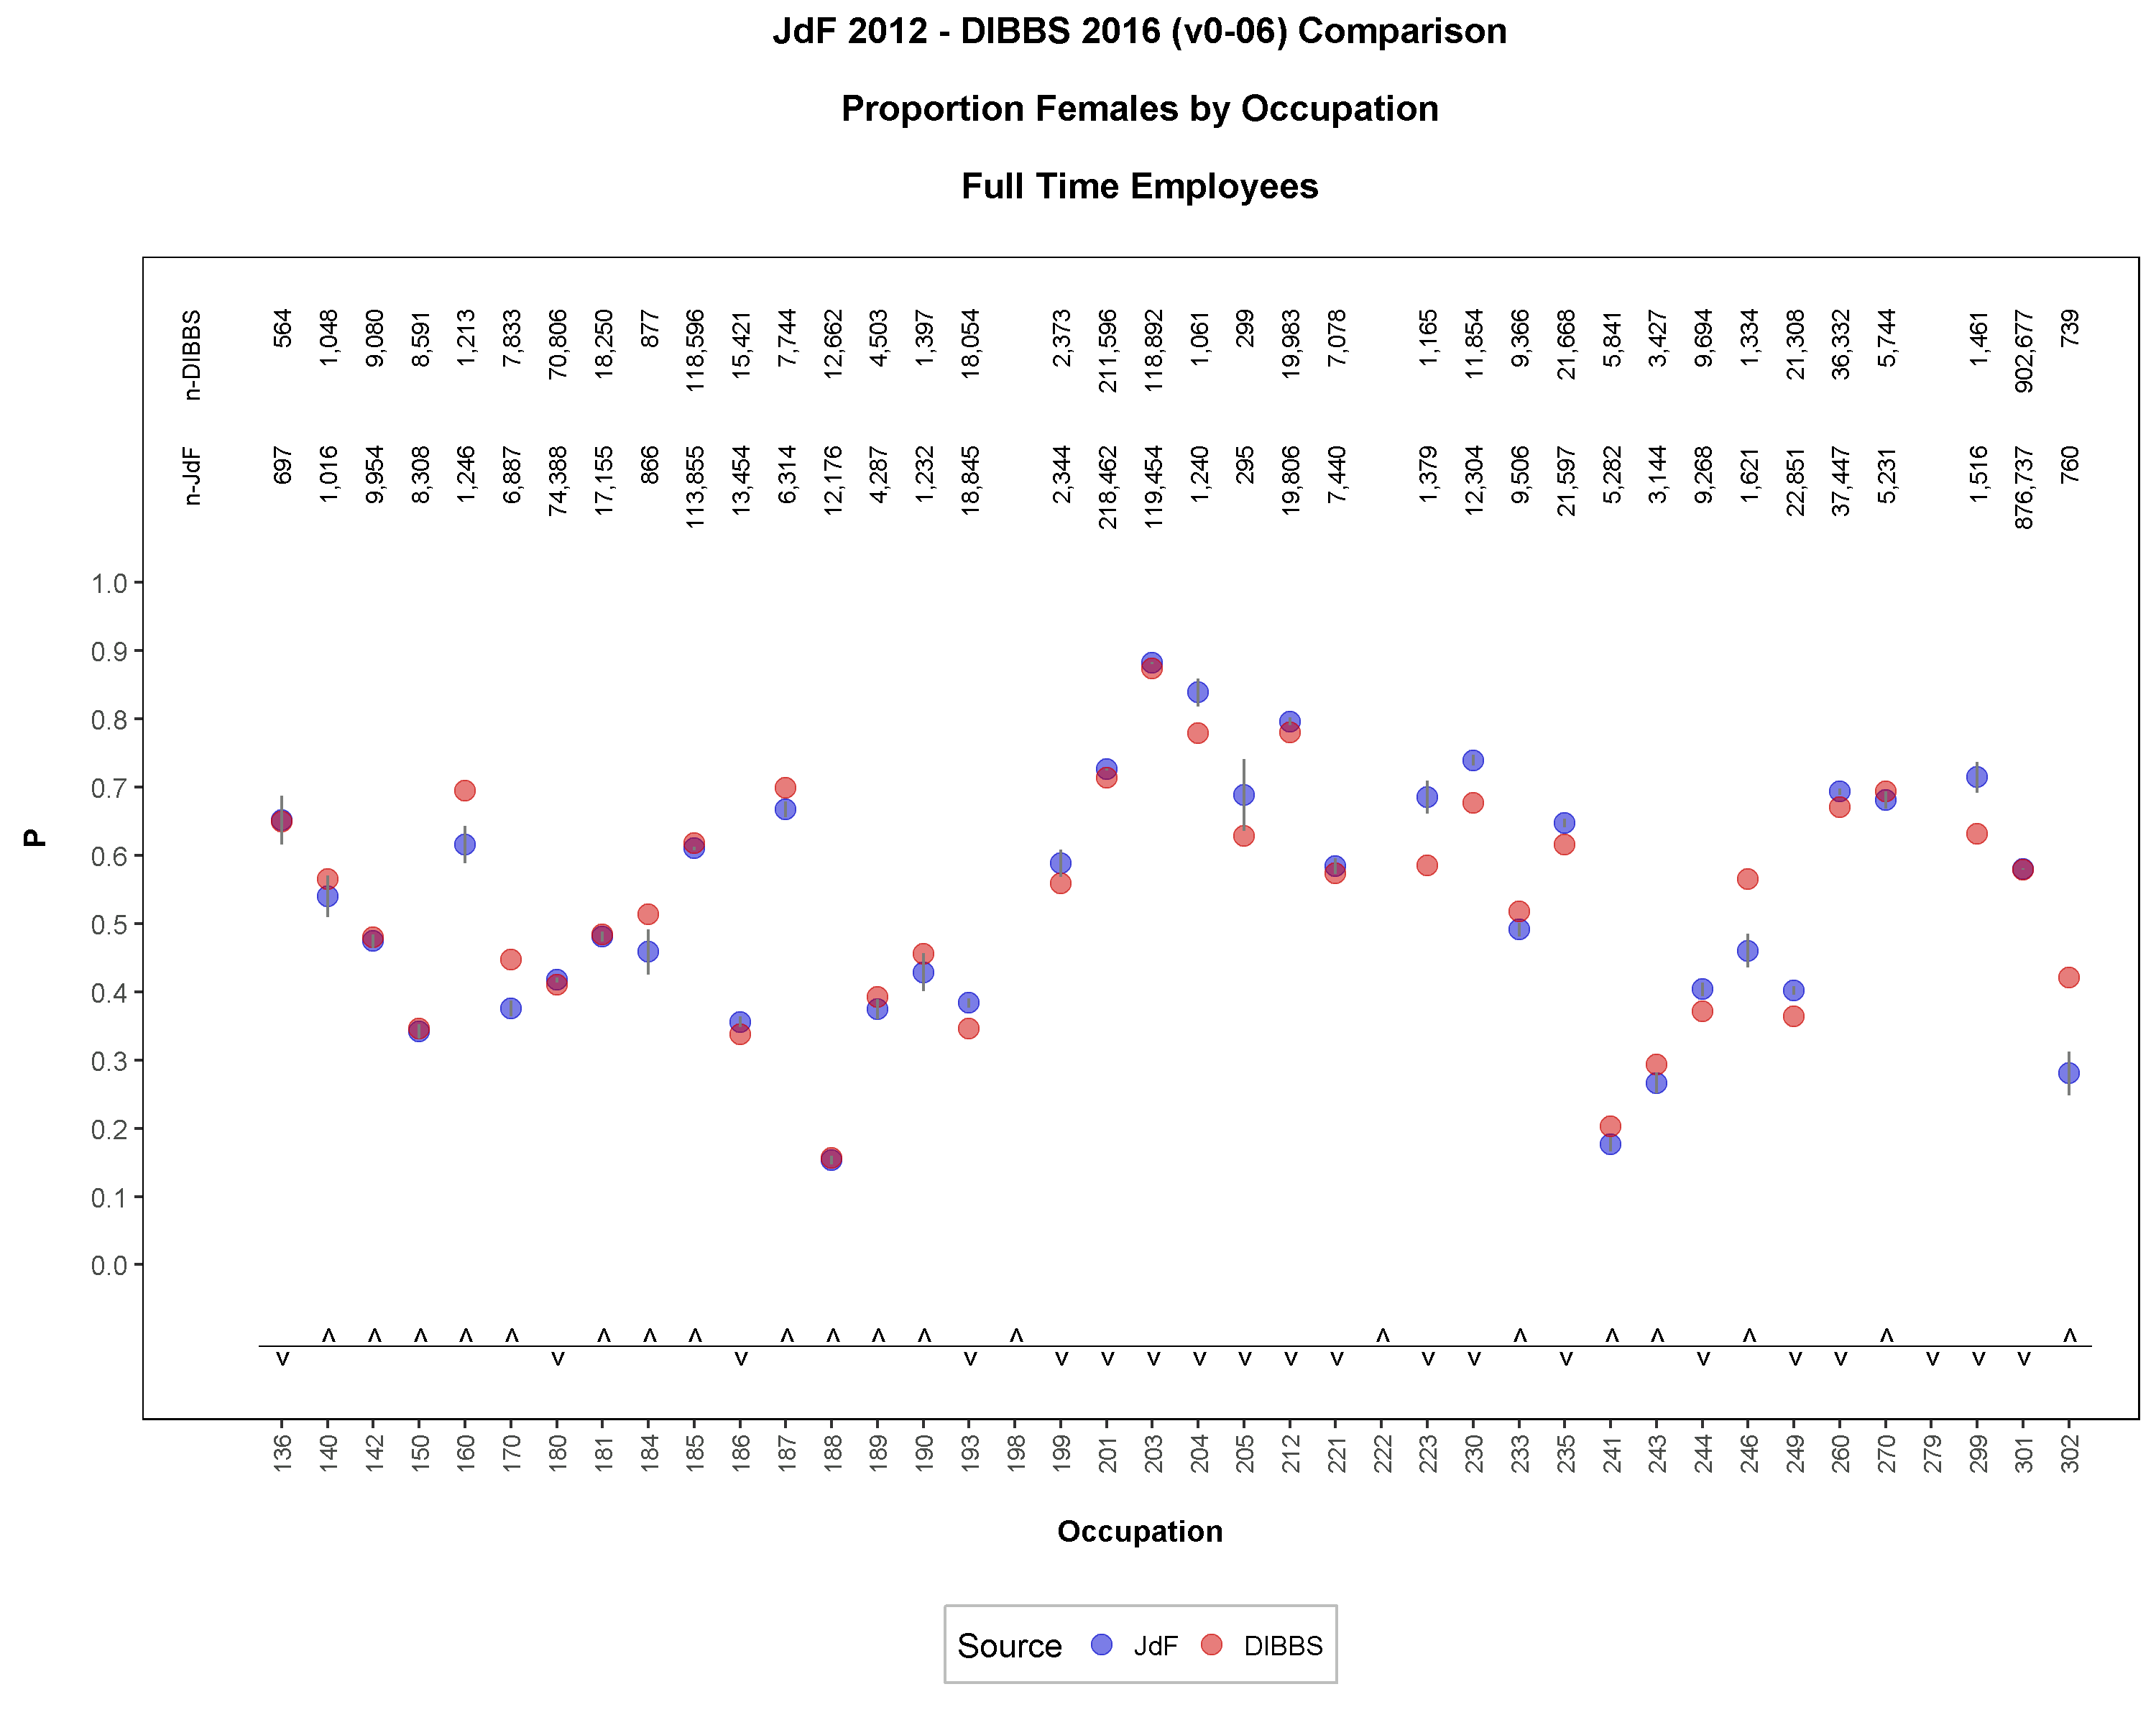
\includegraphics[width=6in, trim={0 1in 0 1in}, clip]{JdFDIBBSOccupationProportionBar41.png}
        \caption{Occupations 0136 through 0302}
        \vspace{10pt}
    \end{subfigure}
    \caption{Proportion female observations by occupation.  All agencies combined.  One synthetic and one authentic point per occupation.}
    \label{figure:JdFDIBBSOccupationProportionBar1}
\end{figure}

\clearpage

\begin{figure}[h]
    \centering
    \begin{subfigure}{1\textwidth}
        \centering
        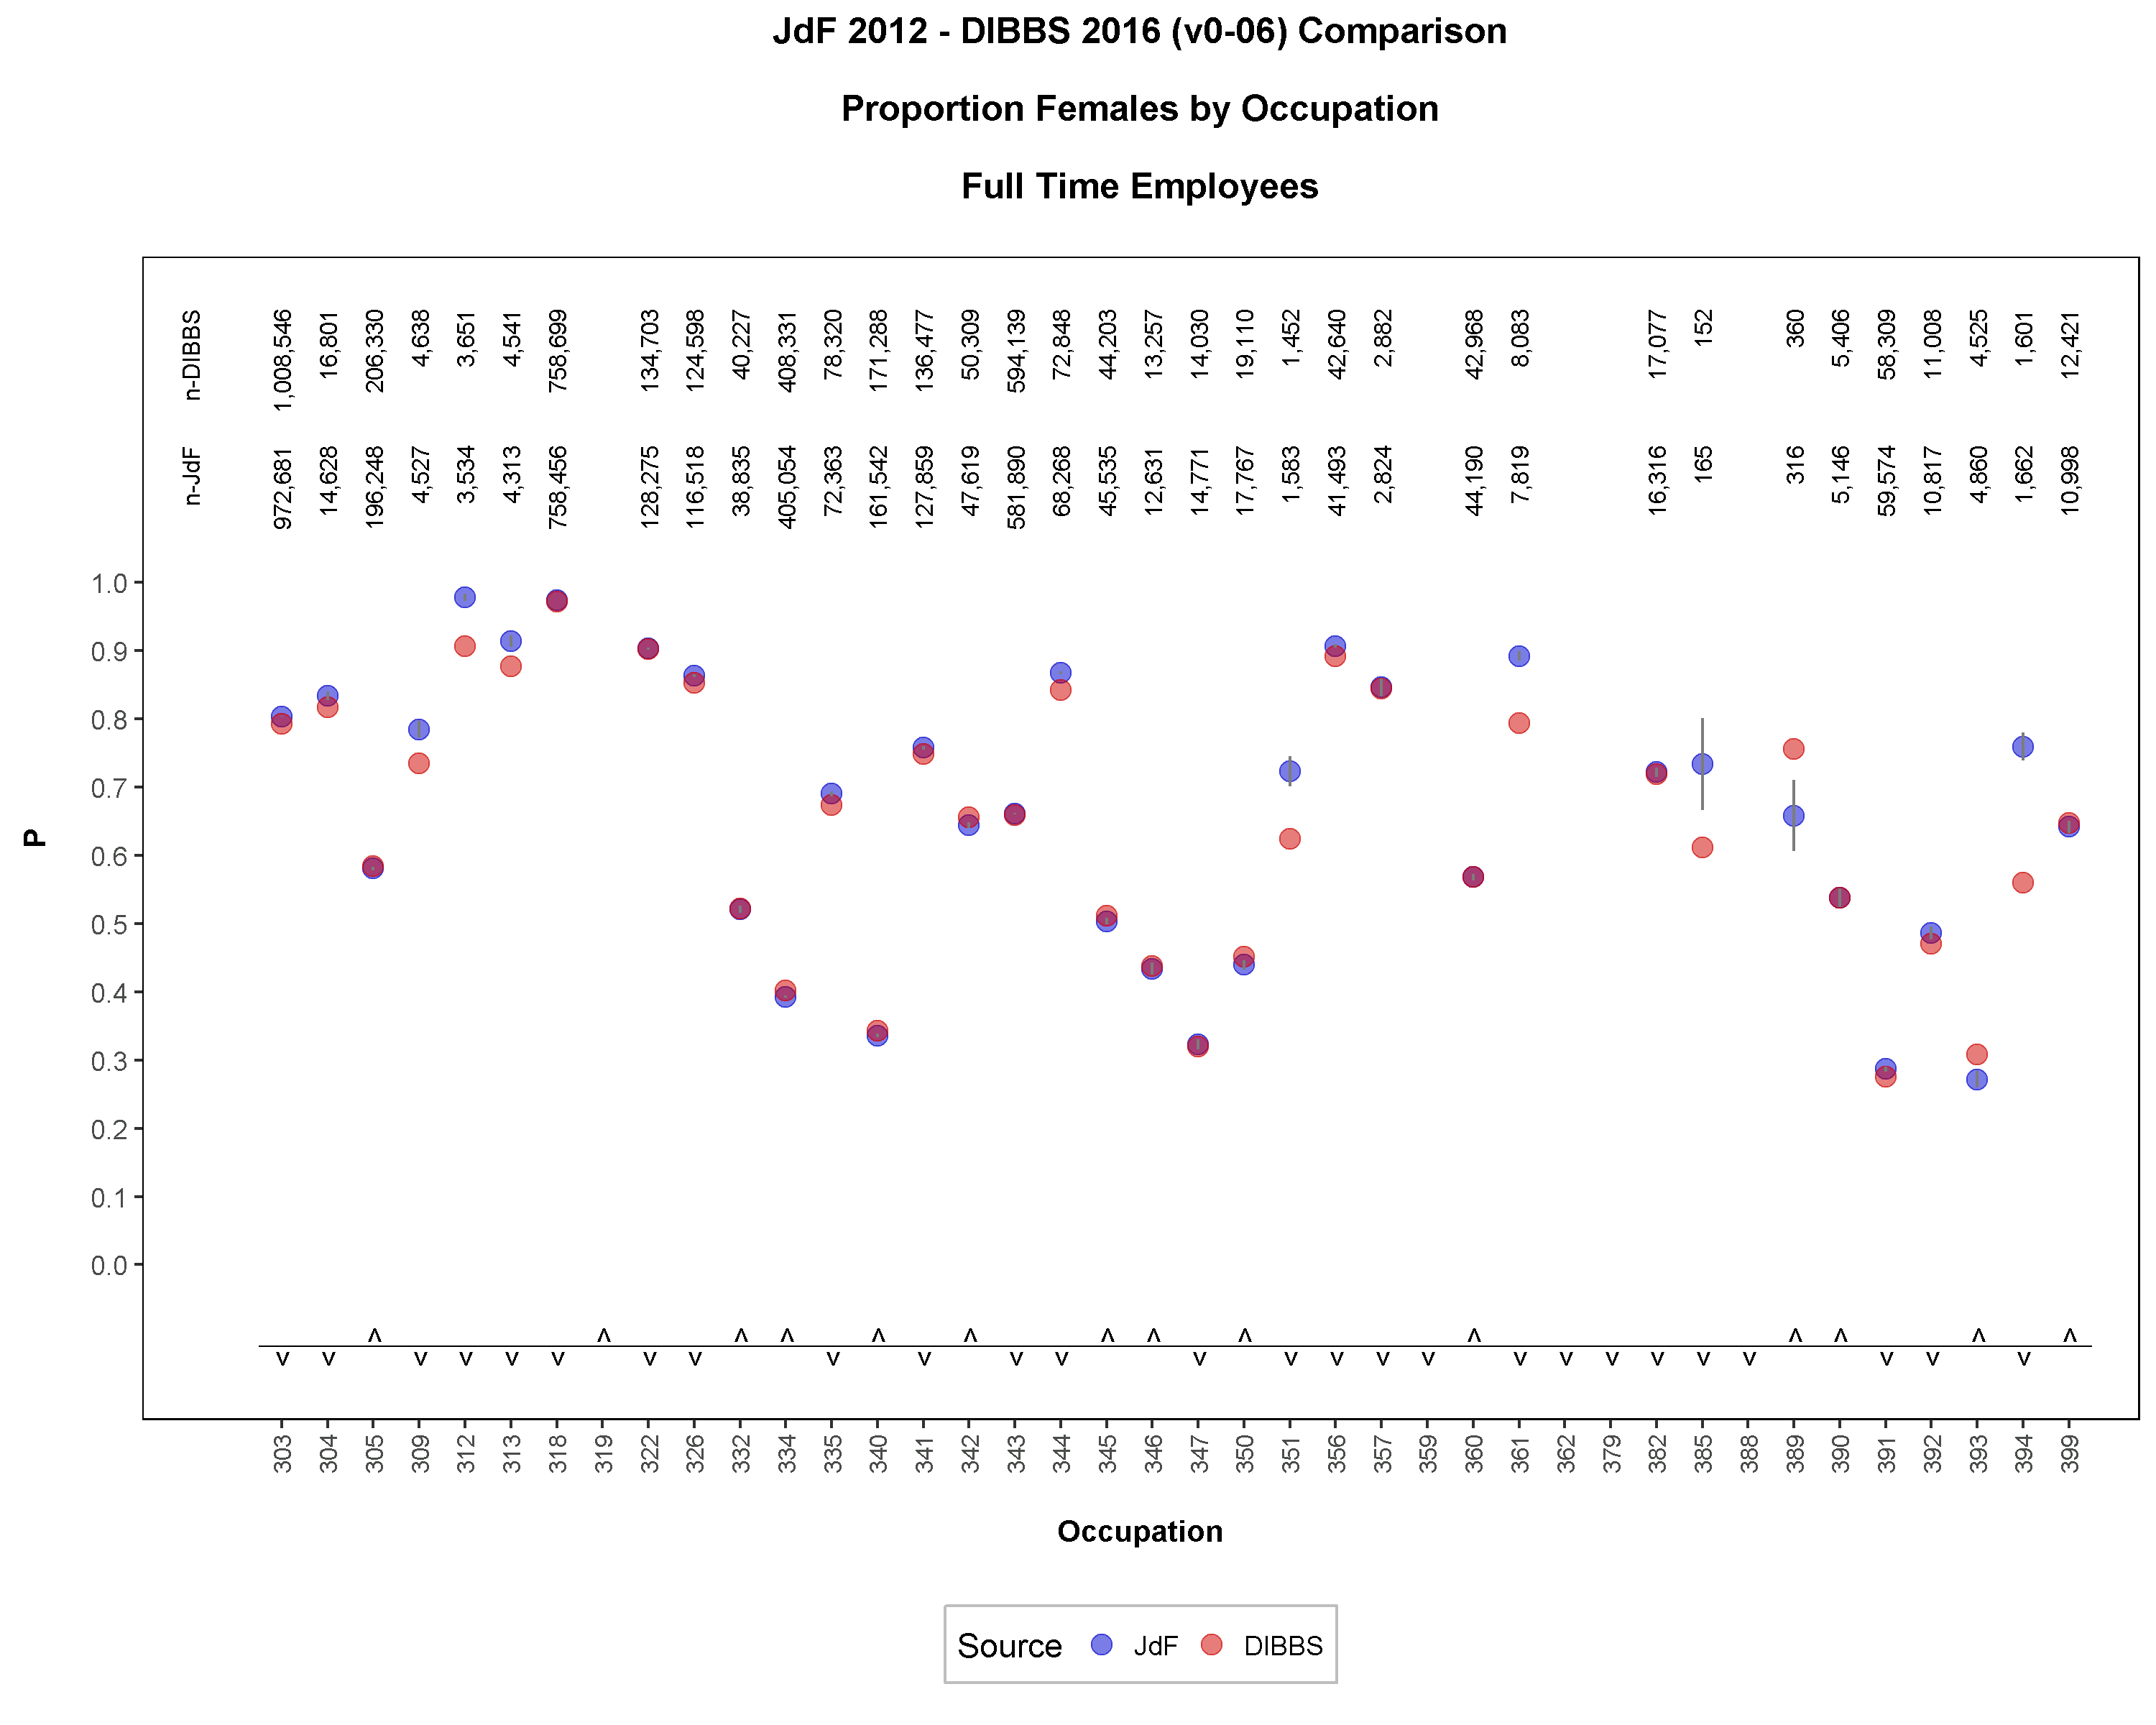
\includegraphics[width=6in, trim={0 1in 0 1in}, clip]{JdFDIBBSOccupationProportionBar81.png}
        \caption{Occupations 0303 through 0399}
        \vspace{10pt}
    \end{subfigure}
    \begin{subfigure}{1\textwidth}
        \centering
        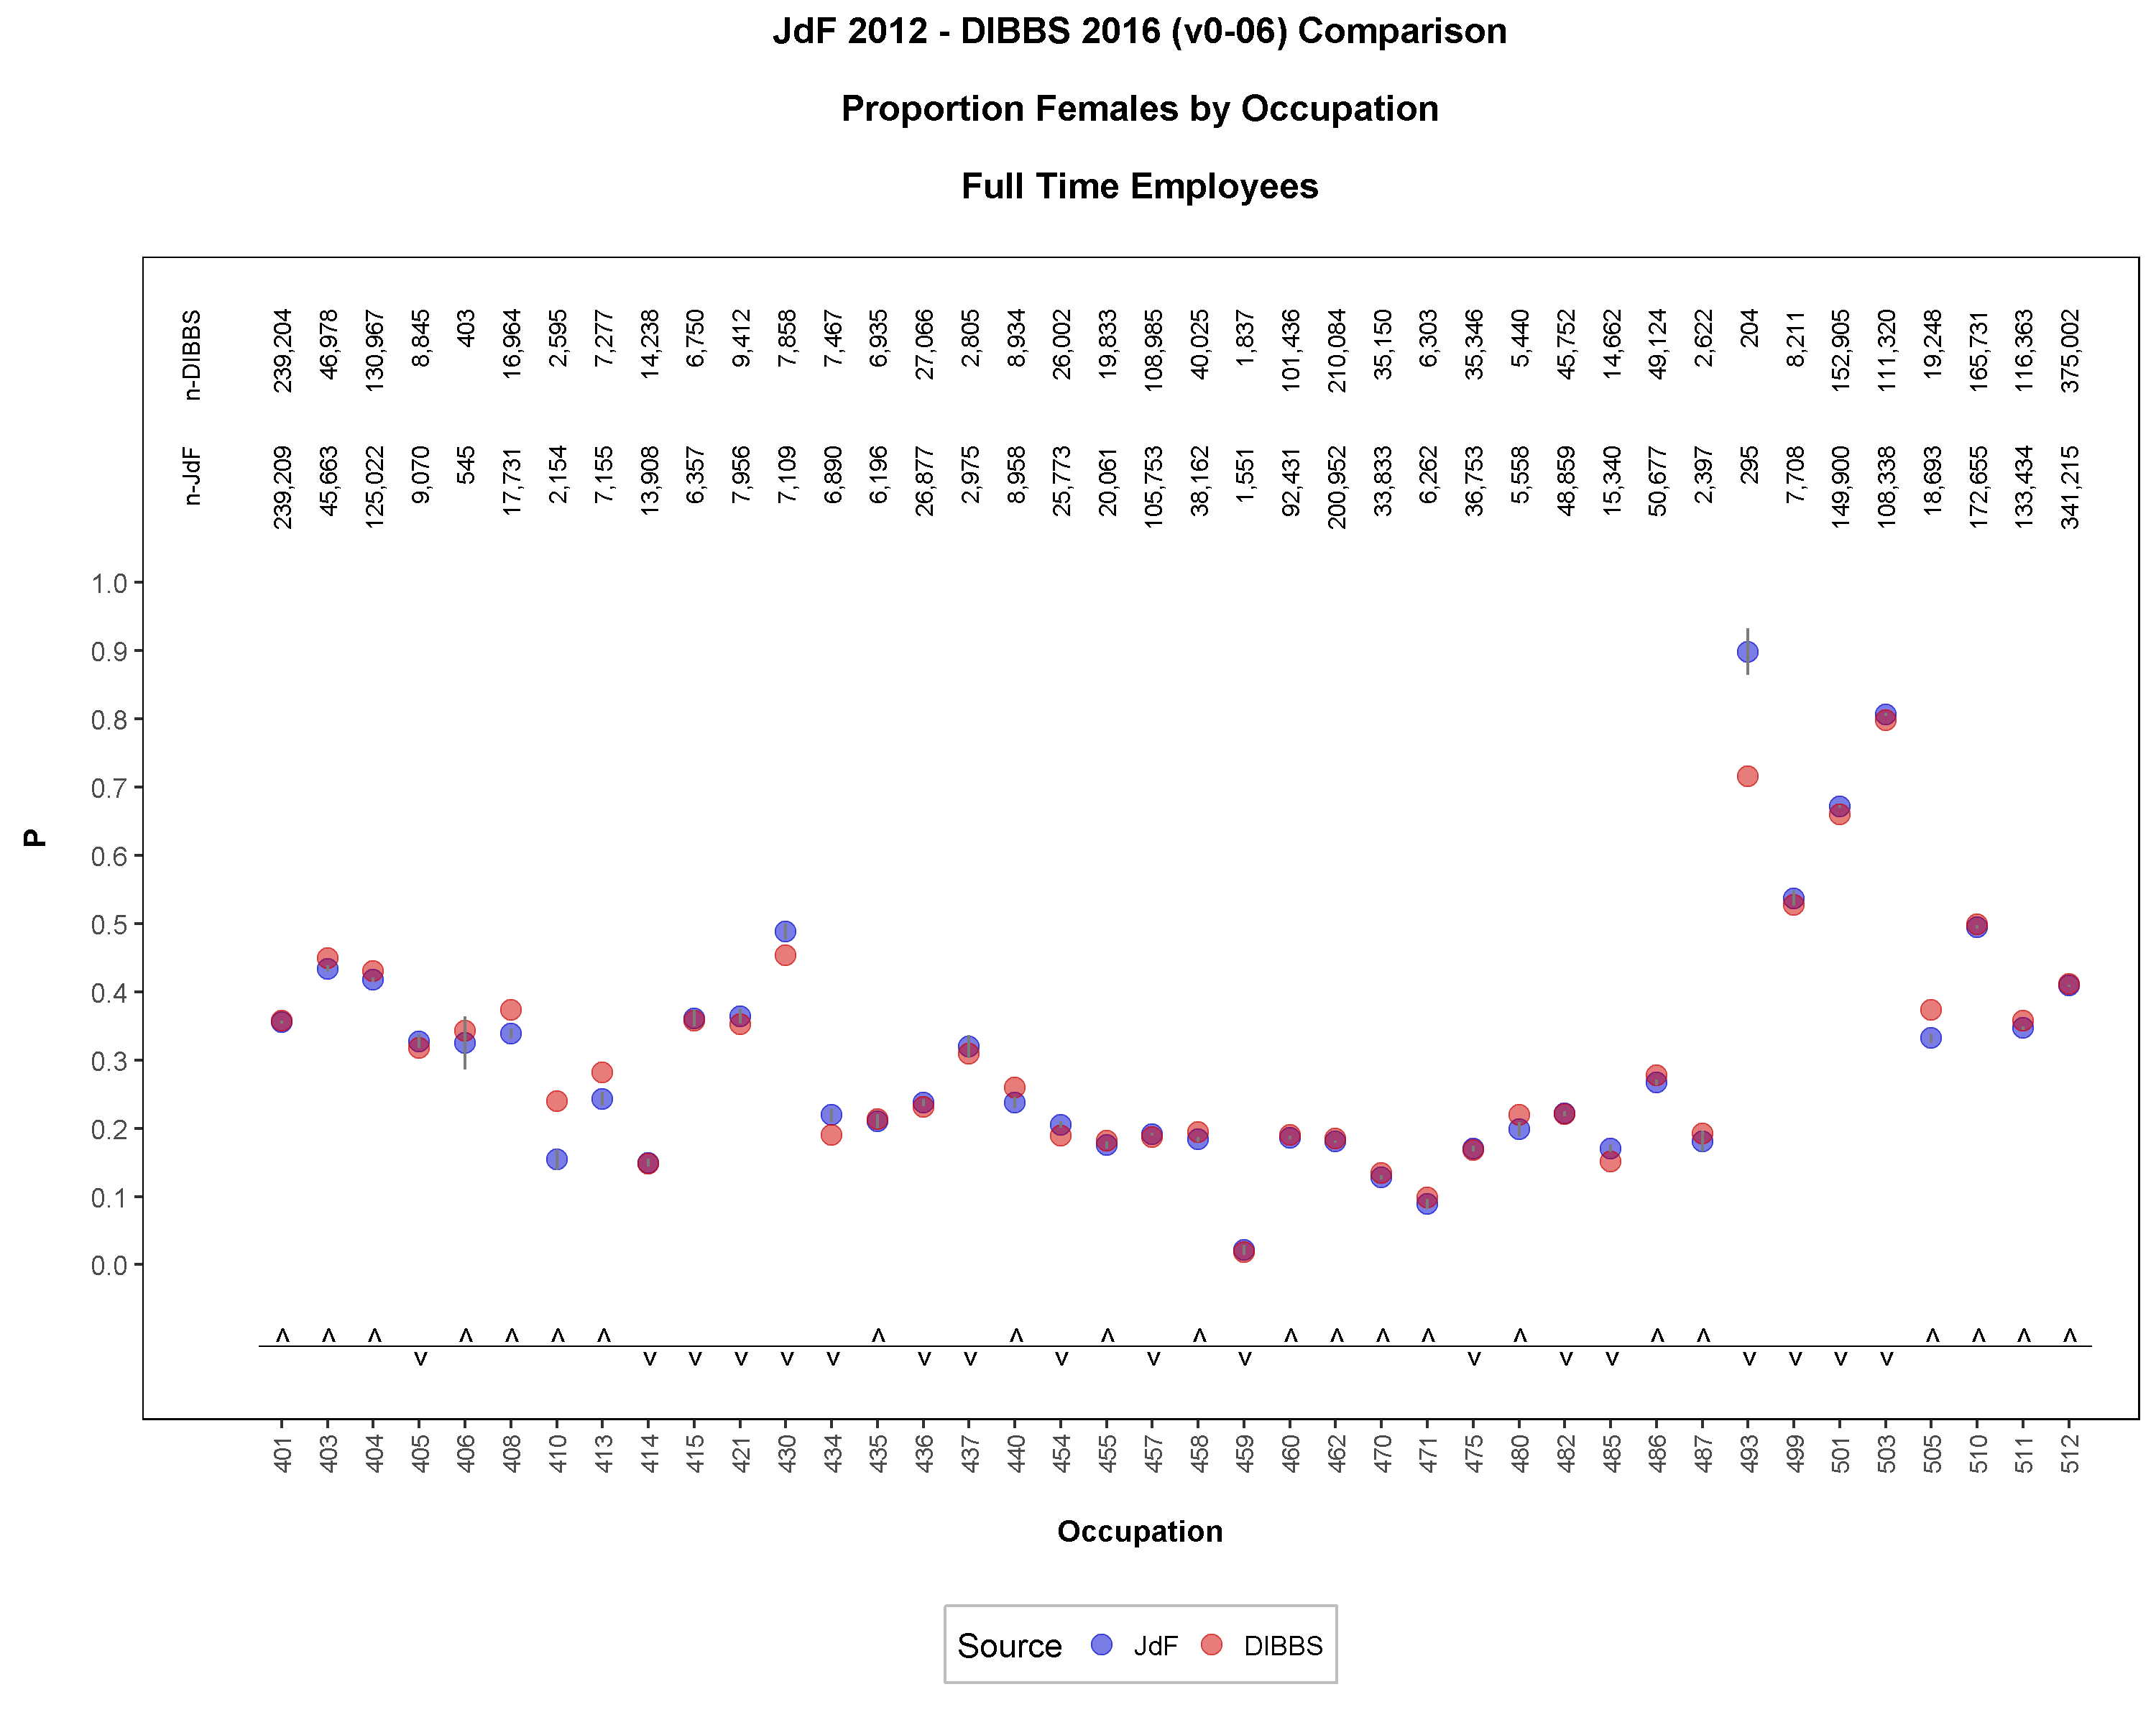
\includegraphics[width=6in, trim={0 1in 0 1in}, clip]{JdFDIBBSOccupationProportionBar121.png}
        \caption{Occupations 0401 through 0512}
        \vspace{10pt}
    \end{subfigure}
    \caption{Proportion female observations by occupation.  All agencies combined.  One synthetic and one authentic point per occupation.}
    \label{figure:JdFDIBBSOccupationProportionBar2}
\end{figure}

\clearpage

\begin{figure}[h]
    \centering
    \begin{subfigure}{1\textwidth}
        \centering
        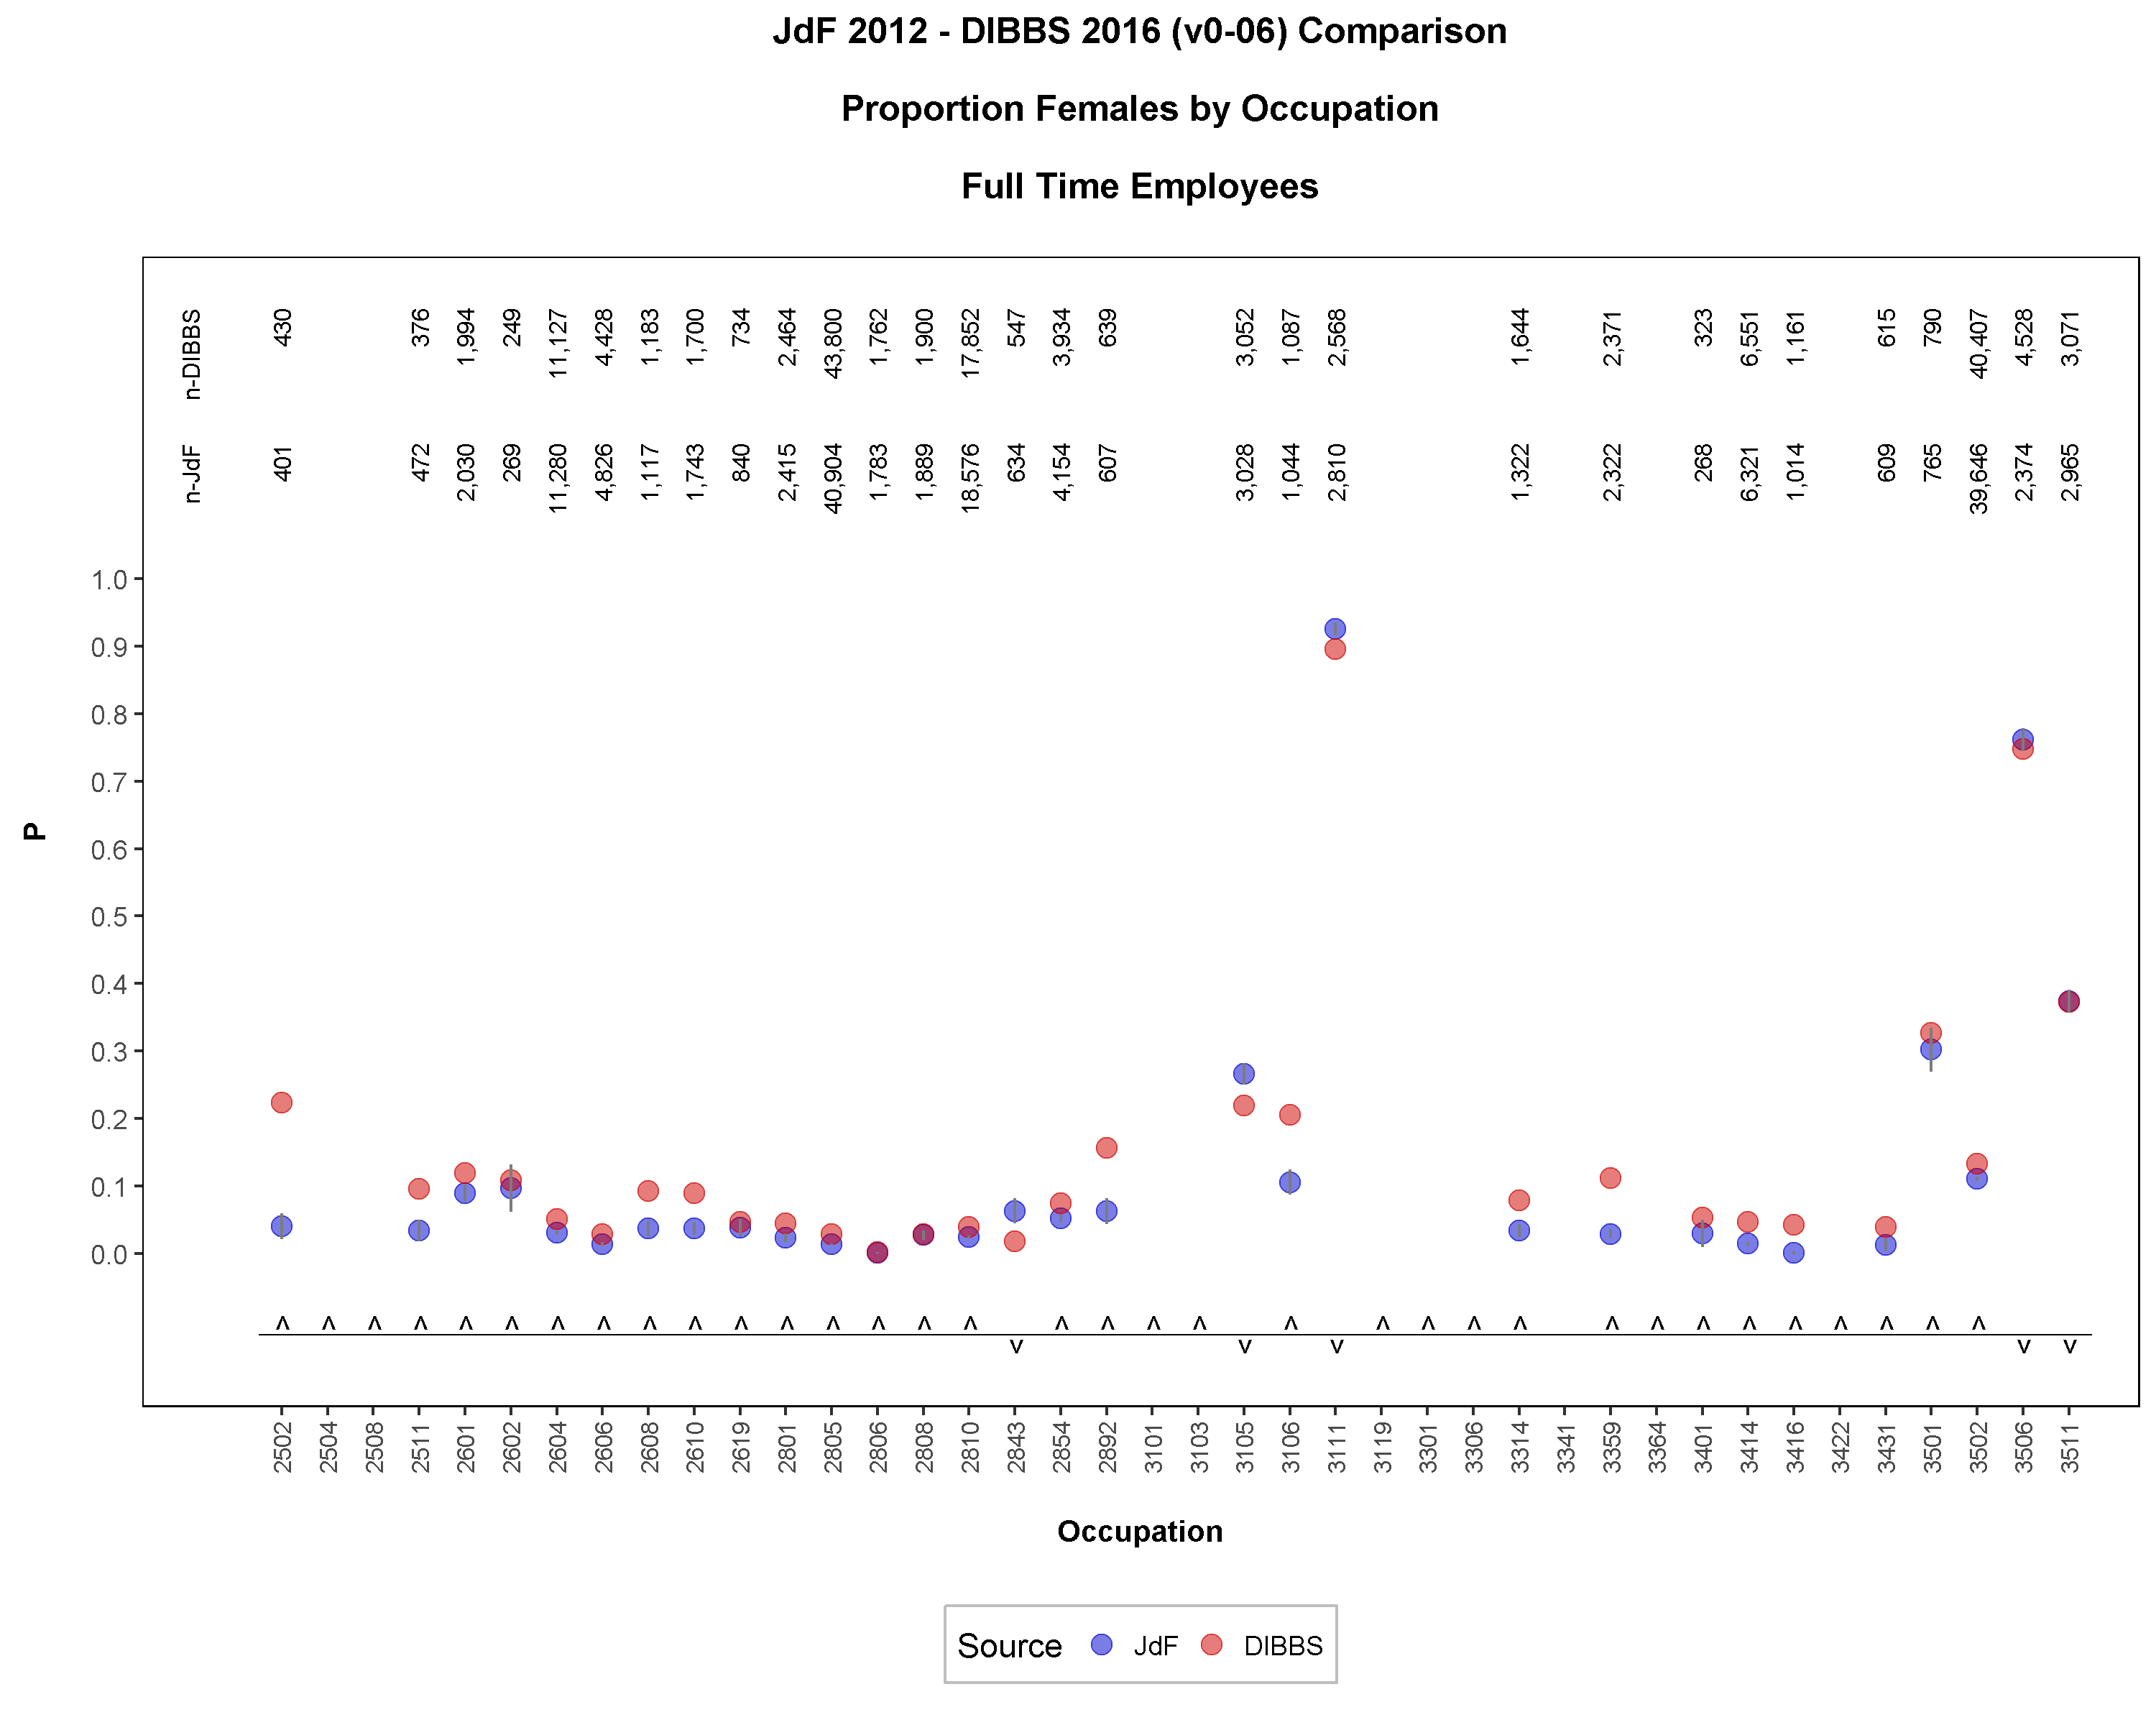
\includegraphics[width=6in, trim={0 1in 0 1in}, clip]{JdFDIBBSOccupationProportionBar481.png}
        \caption{Occupations 2502 through 3511 (trades)}
        \vspace{10pt}
    \end{subfigure}
    \begin{subfigure}{1\textwidth}
        \centering
        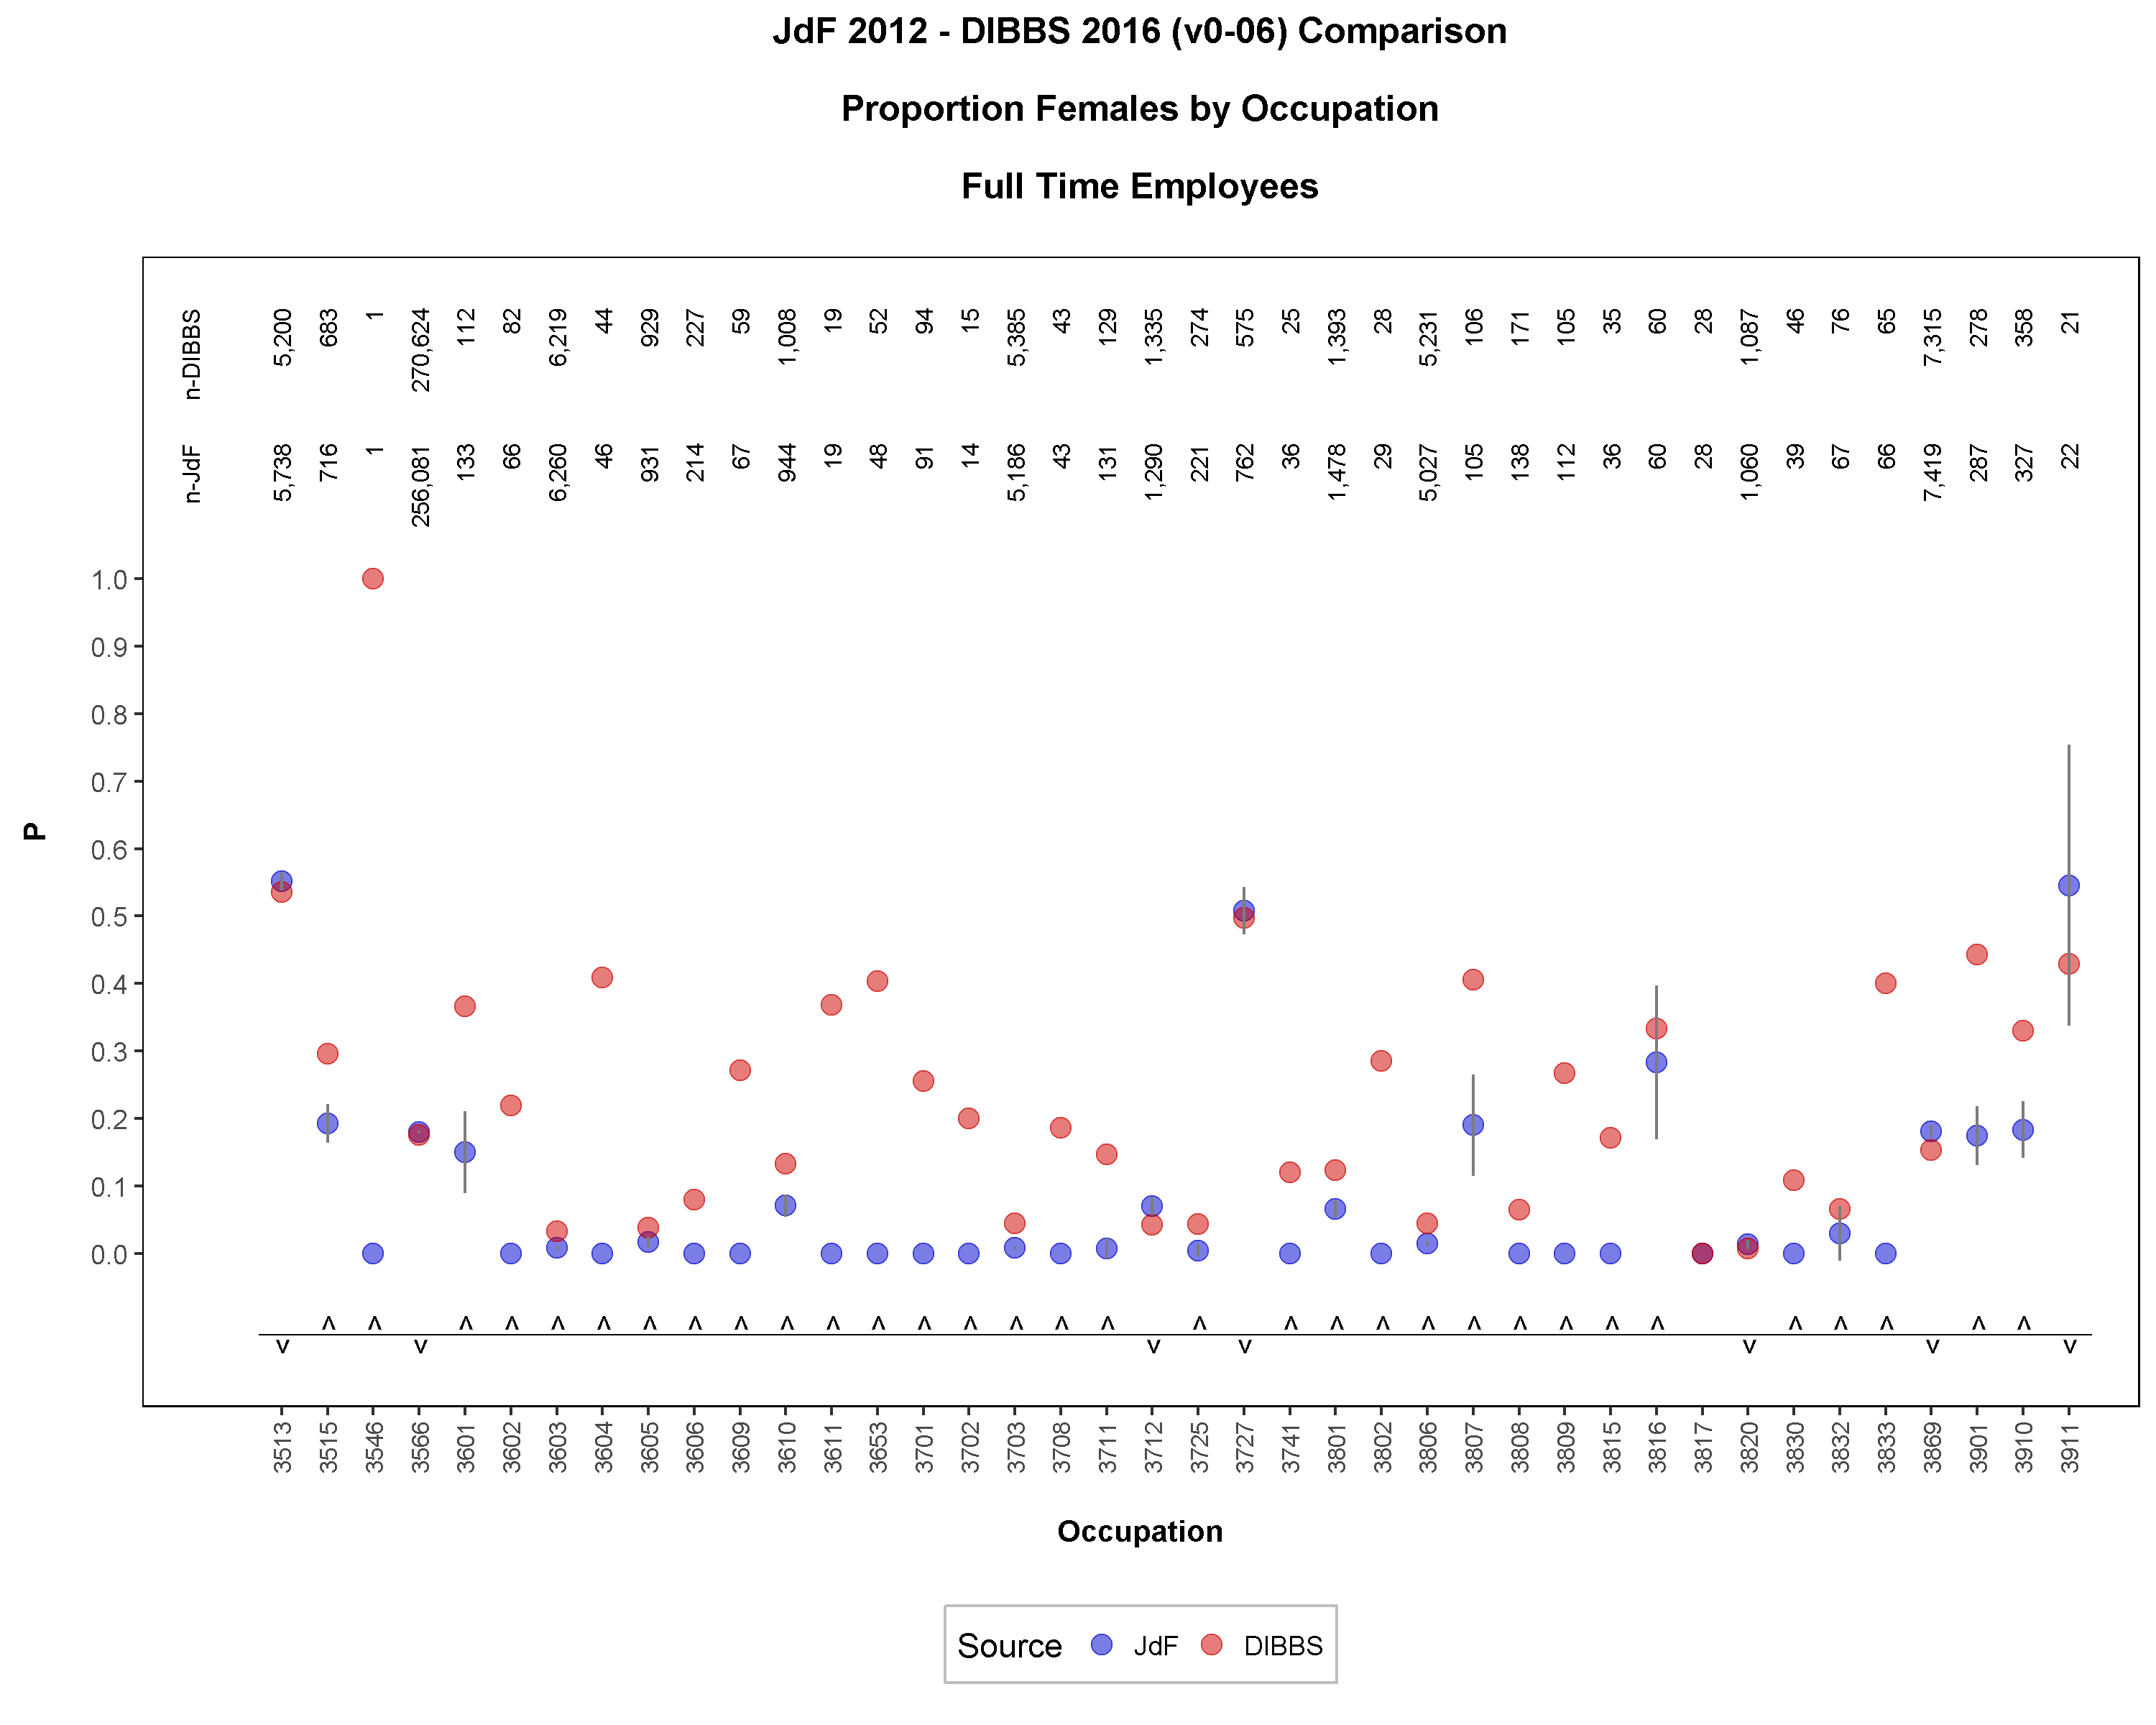
\includegraphics[width=6in, trim={0 1in 0 1in}, clip]{JdFDIBBSOccupationProportionBar521.png}
        \caption{Occupations 3513 through 3911 (trades)}
        \vspace{10pt}
    \end{subfigure}
    \caption{Proportion female observations by occupation.  All agencies combined.  One synthetic and one authentic point per occupation.}
    \label{figure:JdFDIBBSOccupationProportionBar3}
\end{figure}

\clearpage

\begin{figure}[h]
    \centering
    \begin{subfigure}{1\textwidth}
        \centering
        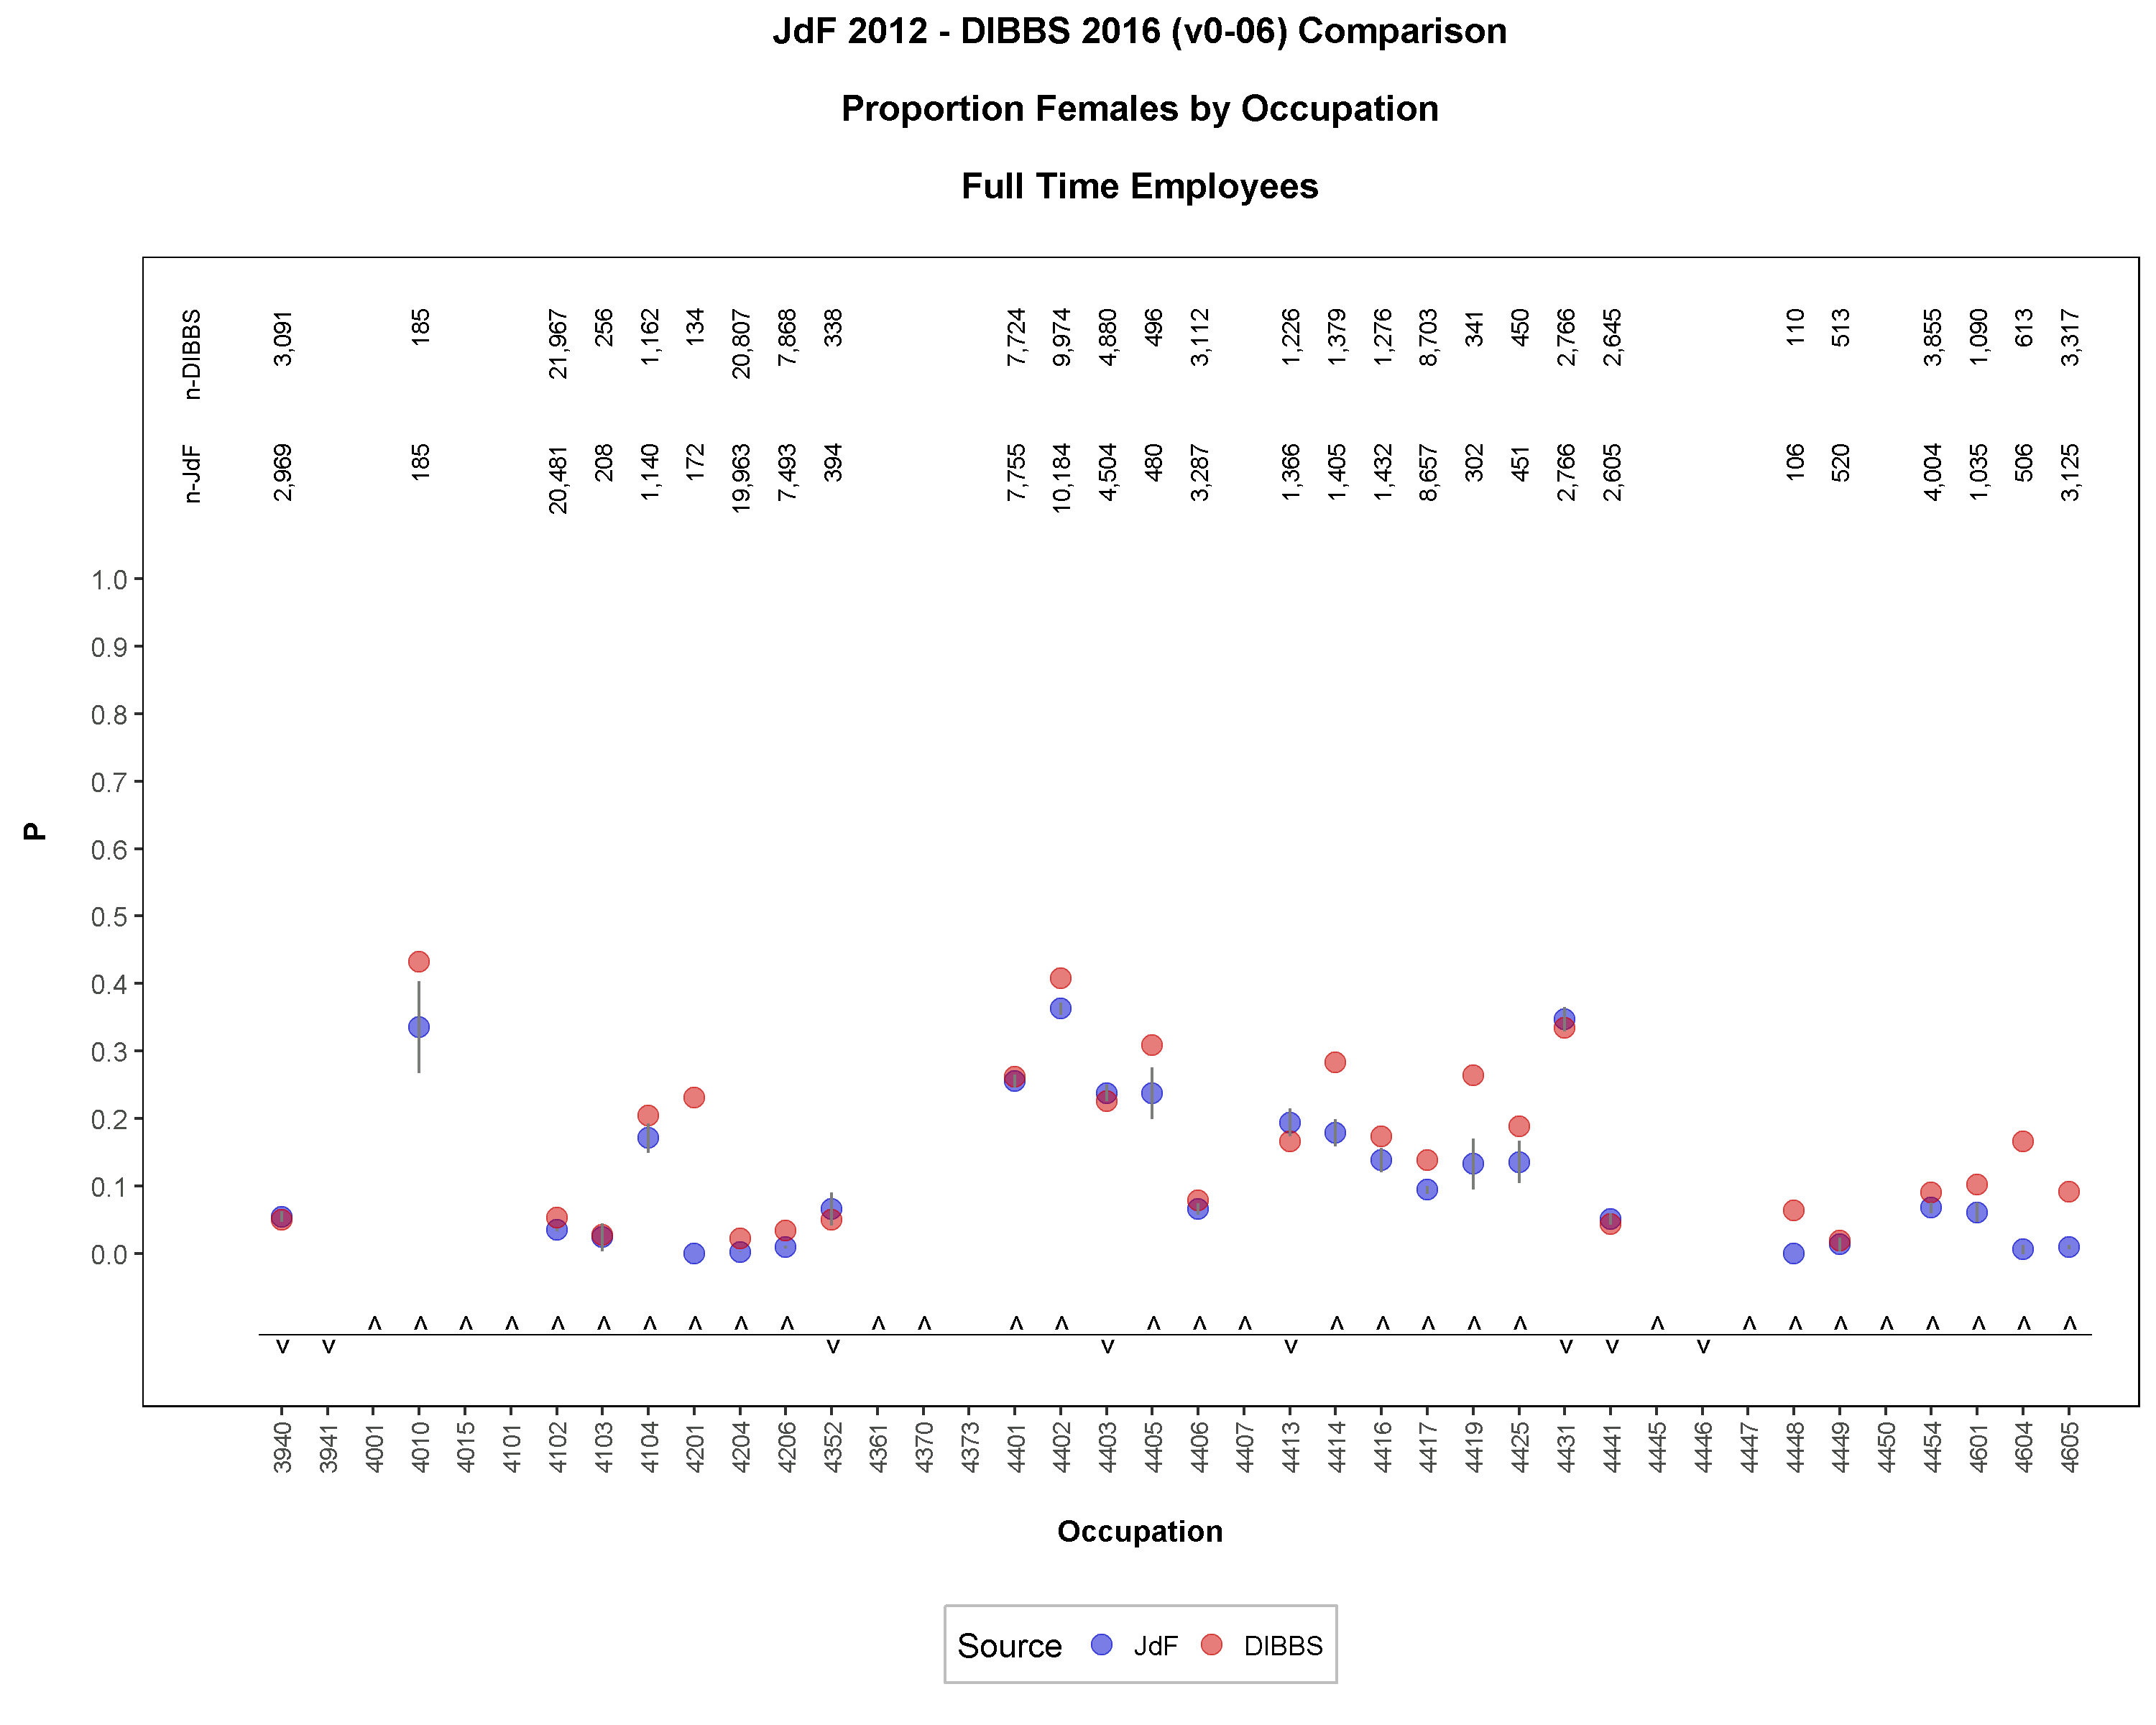
\includegraphics[width=6in, trim={0 1in 0 1in}, clip]{JdFDIBBSOccupationProportionBar561.png}
        \caption{Occupations 3940 through 4605 (trades)}
        \vspace{10pt}
    \end{subfigure}
    \begin{subfigure}{1\textwidth}
        \centering
        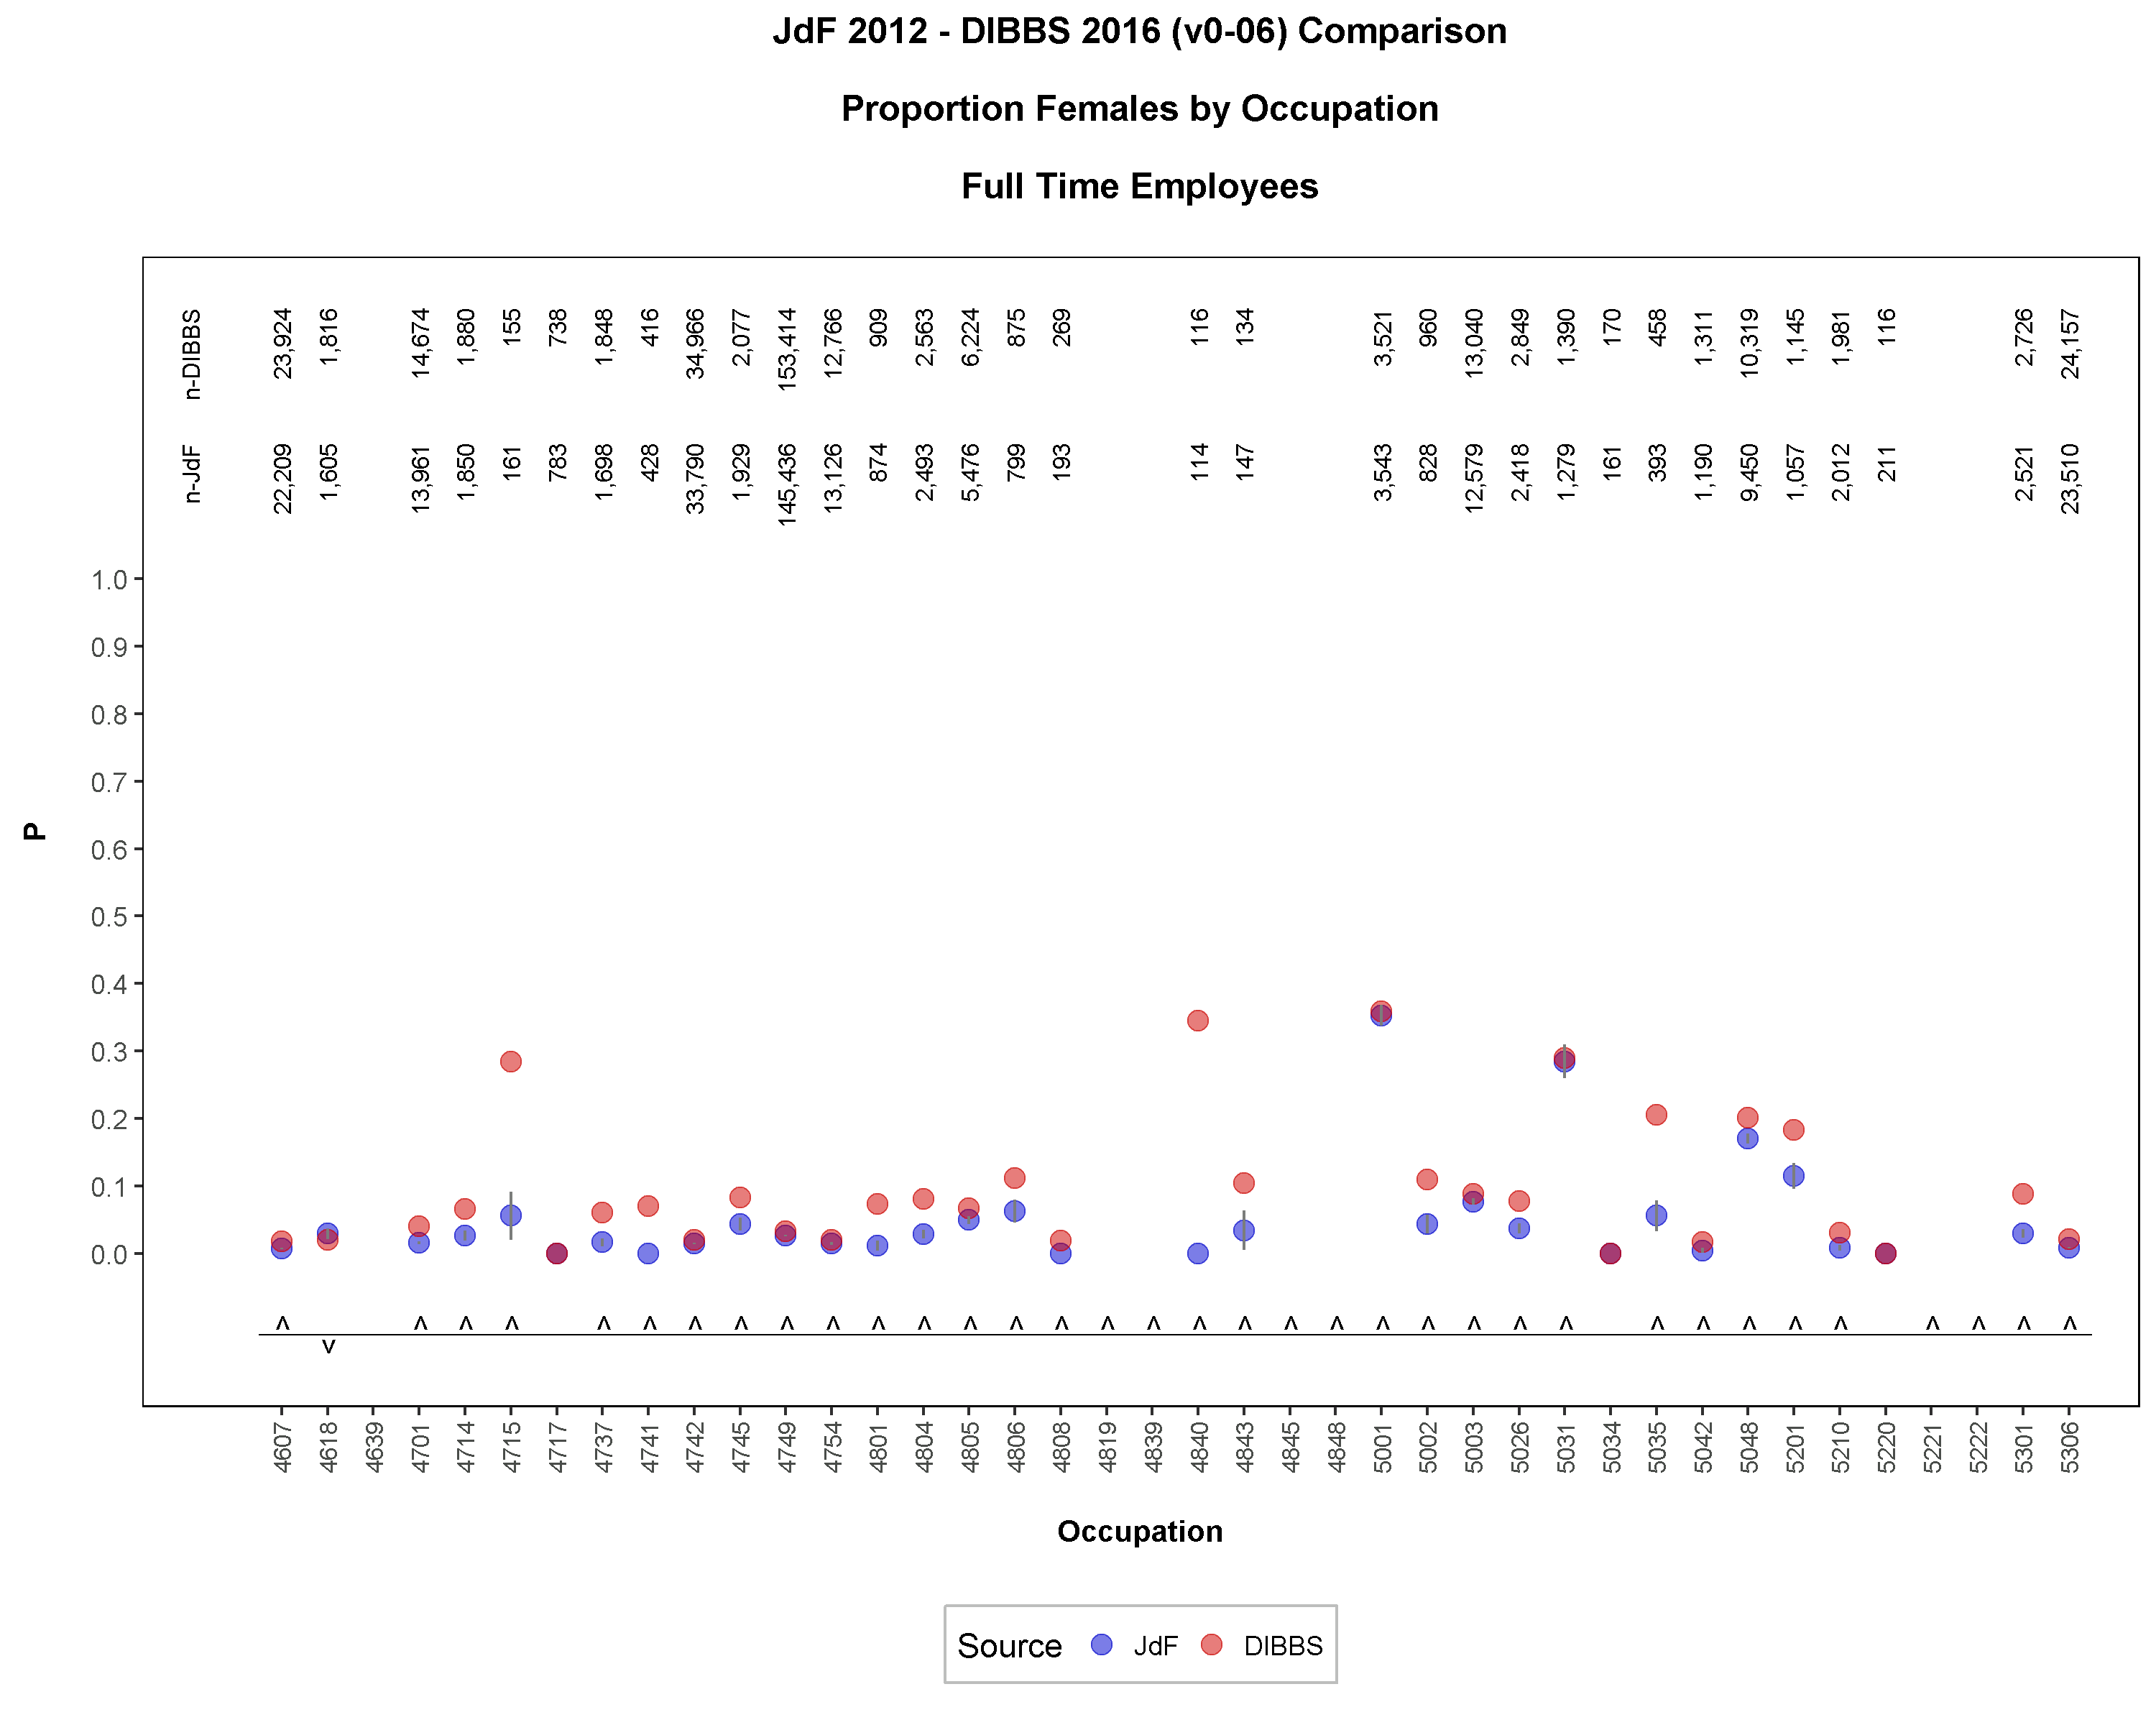
\includegraphics[width=6in, trim={0 1in 0 1in}, clip]{JdFDIBBSOccupationProportionBar601.png}
        \caption{Occupations 4607 through 5306 (trades)}
        \vspace{10pt}
    \end{subfigure}
    \caption{Proportion female observations by occupation.  All agencies combined.  One synthetic and one authentic point per occupation.}
    \label{figure:JdFDIBBSOccupationProportionBar4}
\end{figure}

\clearpage

OCCUPATION GENDER PROPORTION KERNEL DISTRIBUTION\\

Figure \ref{figure:JdFDIBBSProportionFemaleDistributionByOccupation-v0-06} superimposes synthetic and authentic kernel density plots of proportion female employees by occupation.\\

Observations:  Trade occupations in authentic data are slightly over-represented for proportions near zero and above 0.75.  There is slight discrepancy in synthetic proportions near 0 and above 0.75, which is compensated for near central proportions.

\begin{figure}[h]
    \centering
    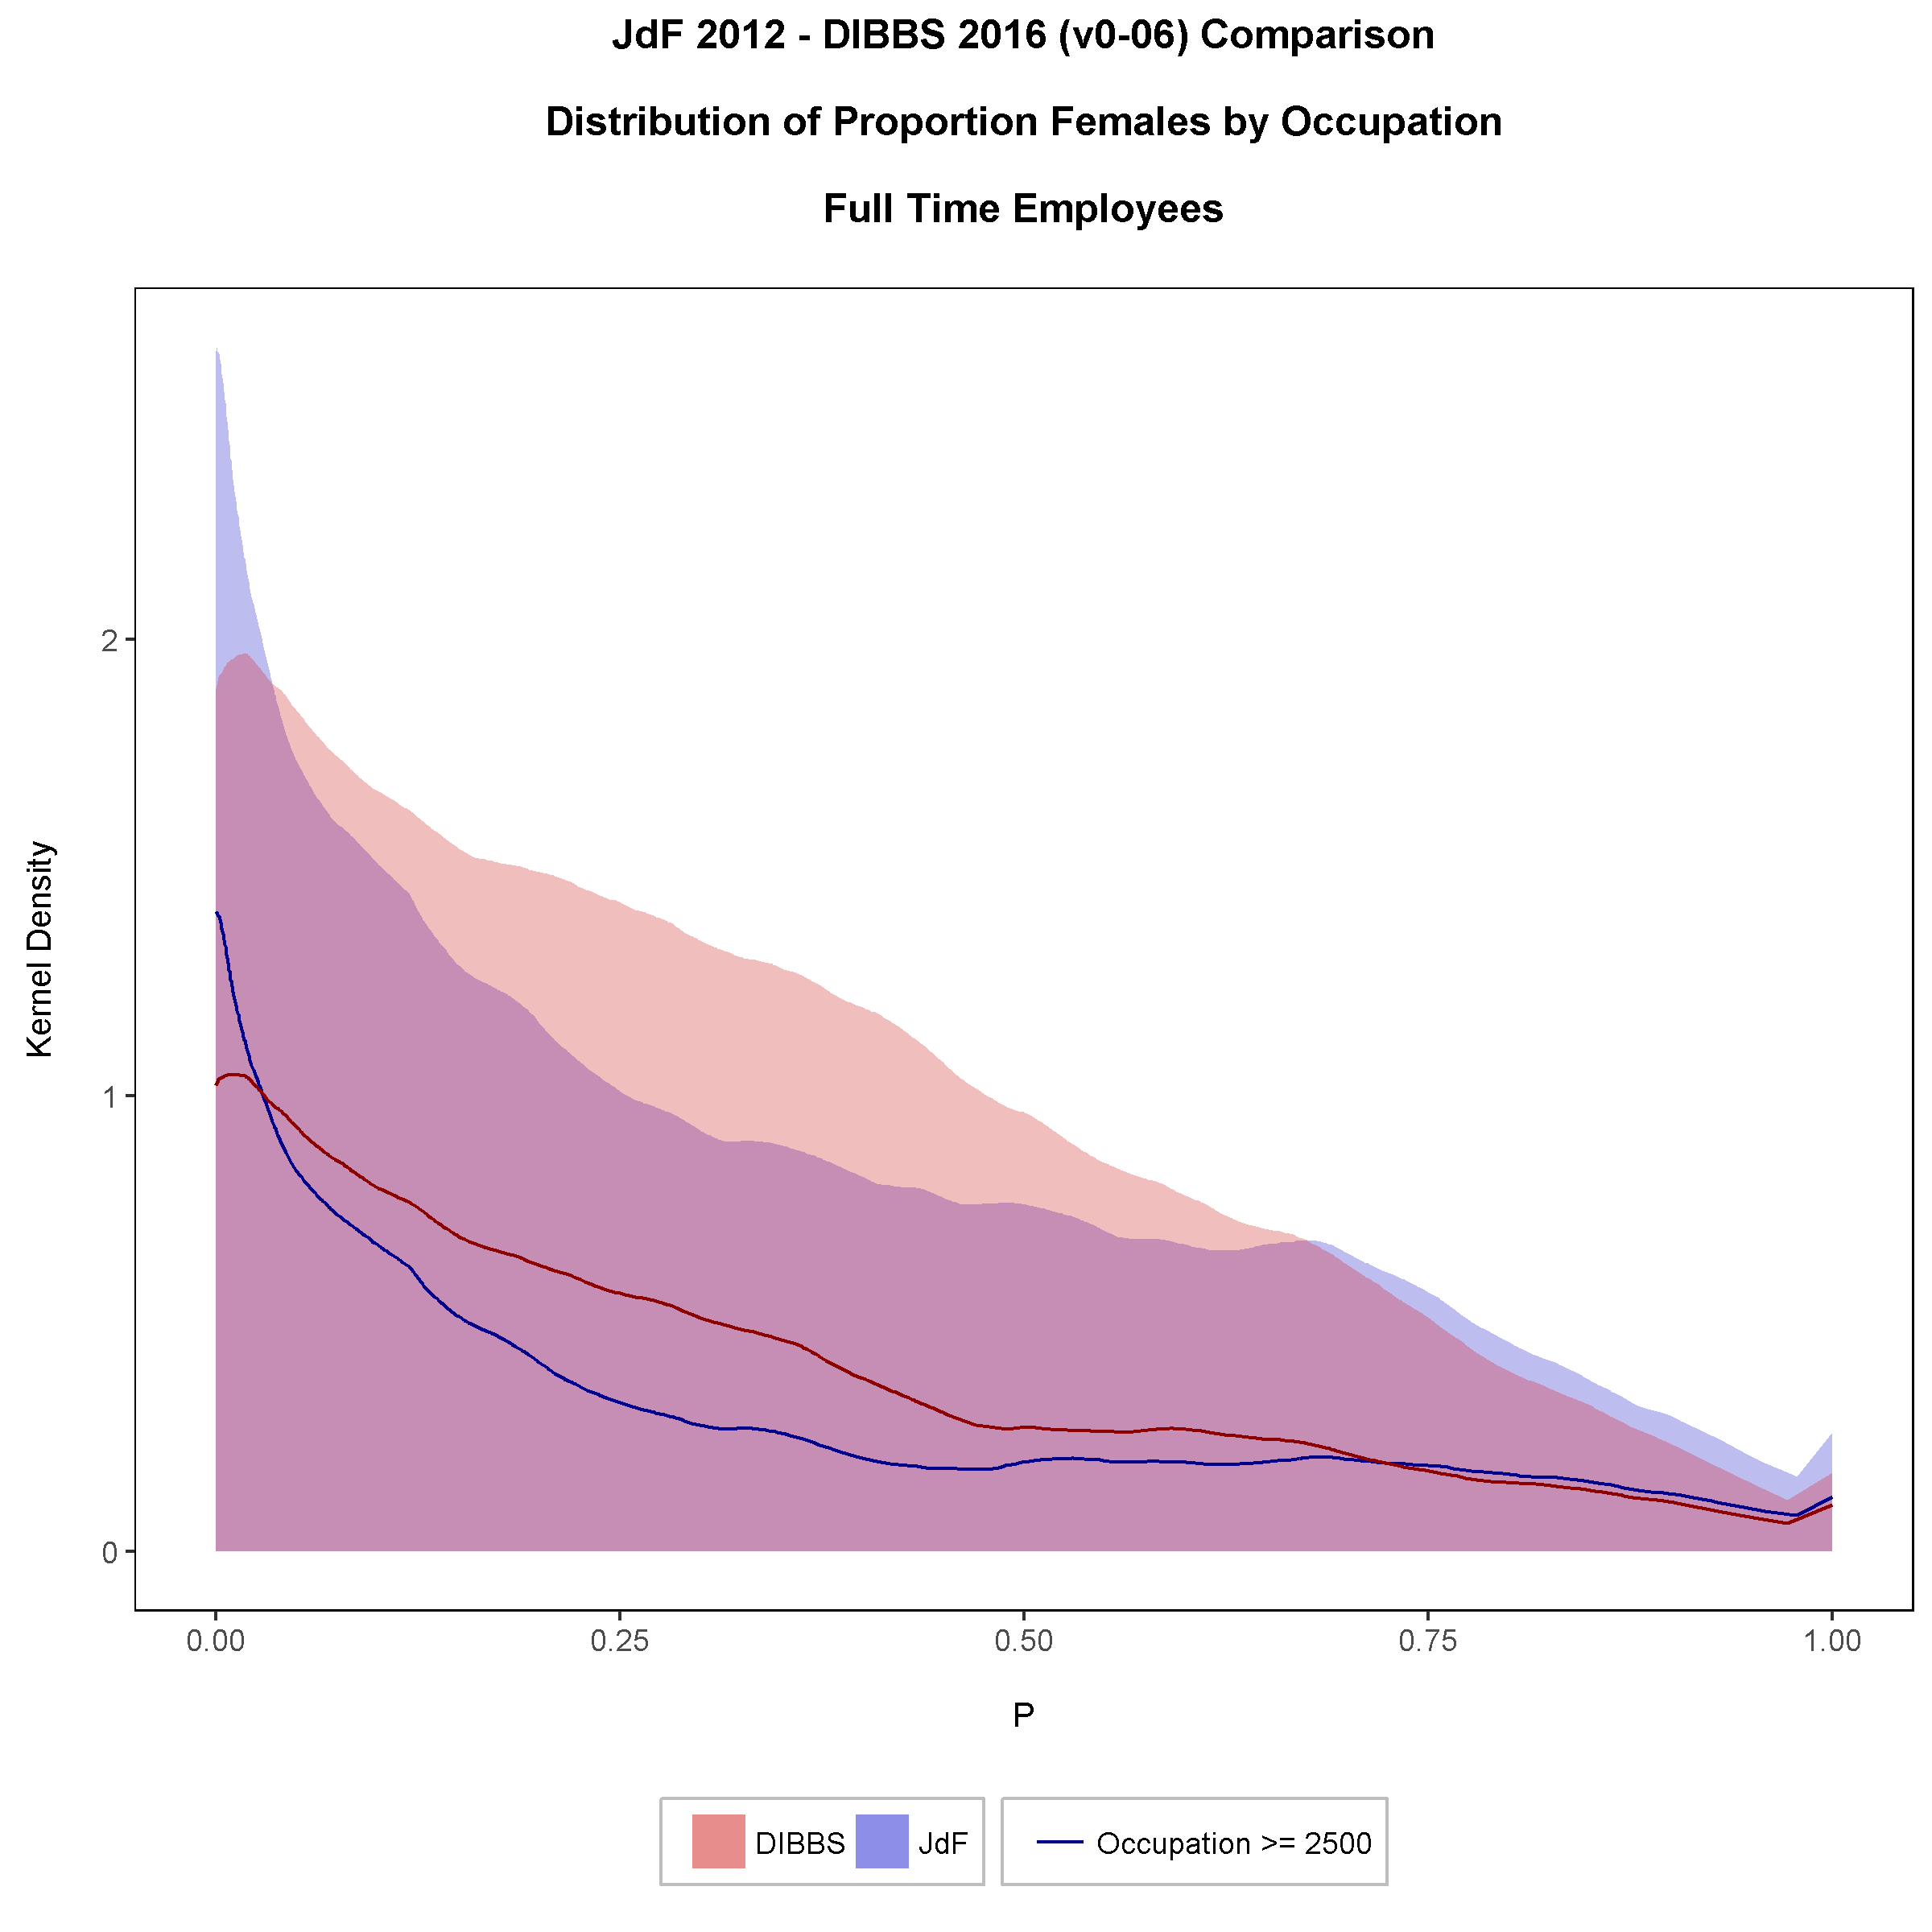
\includegraphics[width=6in, trim={0 0 0 1in}, clip]{JdFDIBBSProportionFemaleDistributionByOccupation-v0-06.png}
    \caption{Occupation proportion female kernel density.  Synthetic and authentic distributions superimposed.  Trade occupations slightly over-represented near zero and above 0.75 in authentic data.  Slight discrepancy in synthetic proportions at extremes.  Compensated for near central proportions.}
    \label{figure:JdFDIBBSProportionFemaleDistributionByOccupation-v0-06}
\end{figure}

\clearpage

GENDER PROPORTION LOGISTIC REGRESSION CLASSIFIER FOR TRADE OCCUPATIONS\\

A gender classifier for occupations with code greater 2500 (trades) using the logistic regression model
\begin{center} $\mest{p}=f(\mest{\beta}_{race}race+\mest{\beta}_{age}age+\mest{\beta}_{age^2}age^2+
    \mest{\beta}_{ed}ed+\mest{\beta}_{ed^2}ed^2+\mest{\beta}_{occ}occ)$,\\
\end{center}
where $f()$ estimates proportion female observations by race, age, education, and occupation, was used to classify sex, such that all observations associated with combinations of independent variables with $\mest{p}\ge$0.5 are classified as female.  Figure \ref{figure:GenderProportionROCAgeAgeSqEdEdSqRaceOccGE2500ByFYv0-06} plots, for fiscal years 1988-2011 (all years supplied by OPM) and $\mest{p}$ values from 0 to 1.0, the proportion of accurate female observation classification (y-axis) against the proportion accurate male classification (x-axis).\\

Observation:  Although the classifiers, exhibiting somewhat flat ROC curves (near the $\mest{p}$=0.5 reference line of slope 1.0) appear to be of limited utility, those derived from synthetic data are nearly identical their counterparts derived from authentic data, including an apparent reduction in utility (nearer to the reference line) as fiscal years advance.  Incidentally, the reduced utility with year may reflect structural changes in proportion female for trade occupations during this period.\\

\begin{figure}[h!]
    \centering
    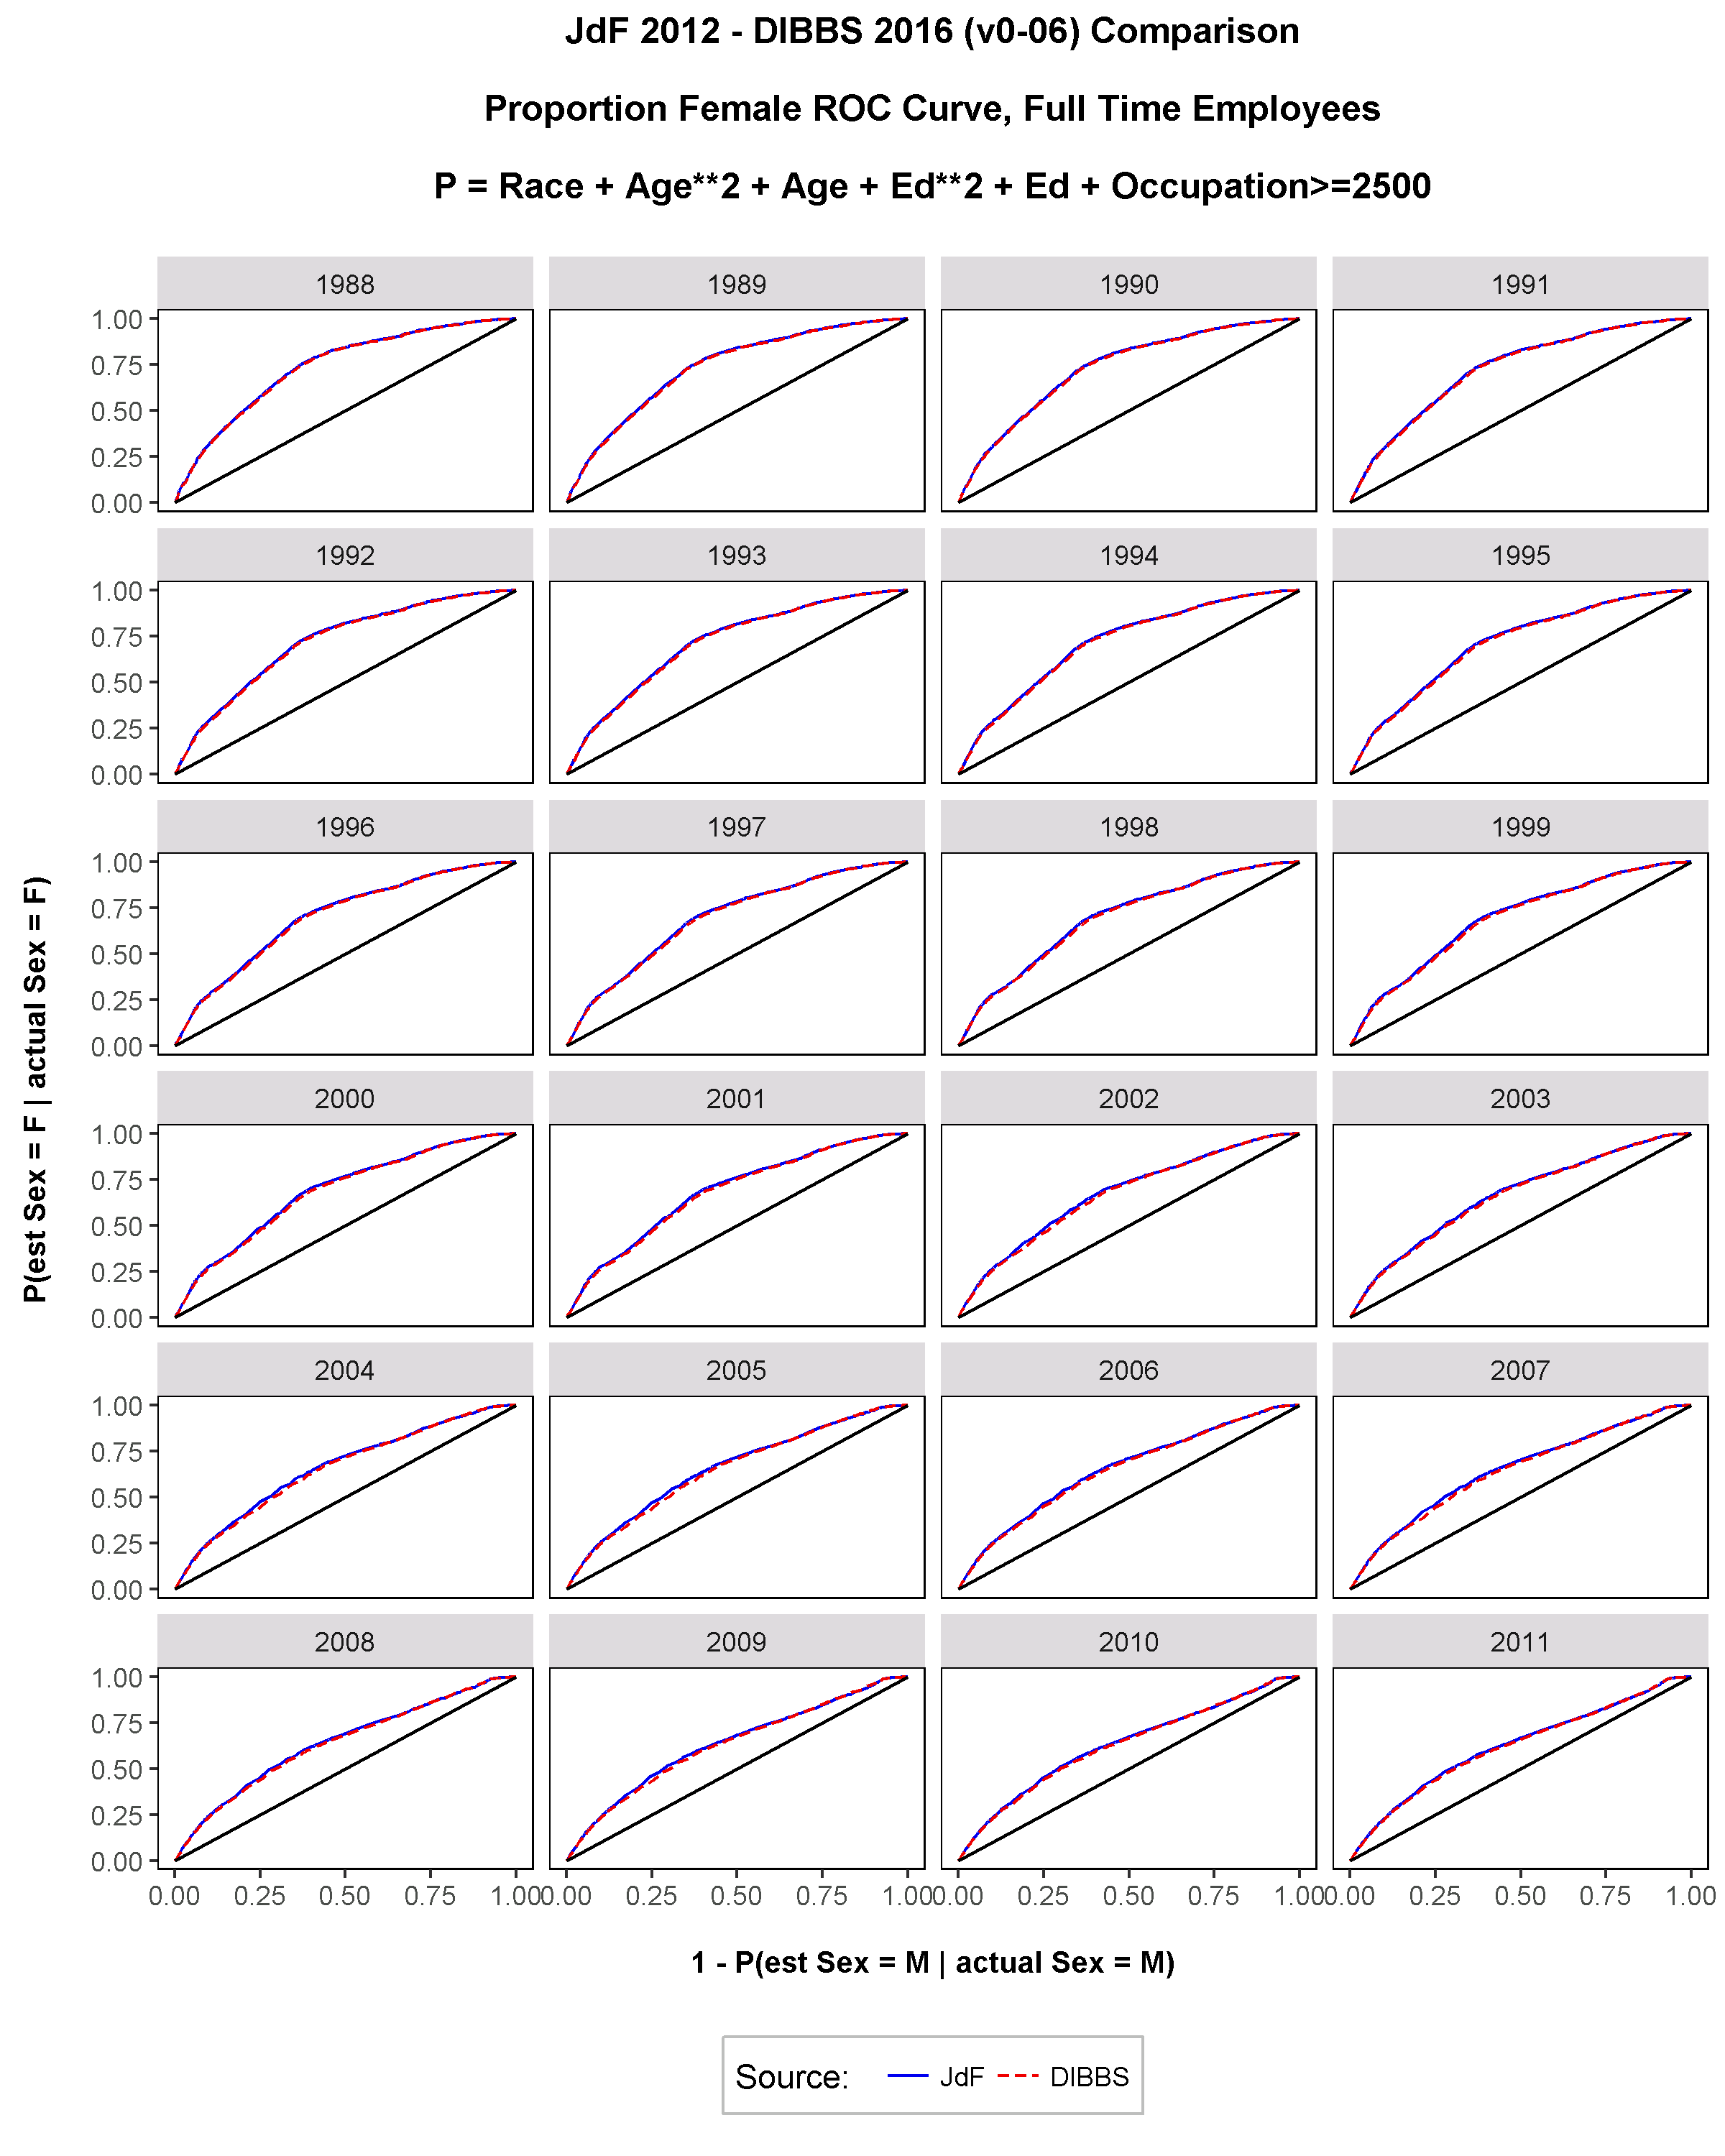
\includegraphics[width=5in, trim={0 0.75in 0 1in}, clip]{GenderProportionROCAgeAgeSqEdEdSqRaceOccGE2500ByFYv0-06.png}
    \caption{Proportion female race, age, education, occupation classifier ROC curves.  One curve per data set per by fiscal.  Agreement in classifier accuracy indicated by overlapping curves. Pattern of decreased accuracy as years progress captured in both data sets. }
    \label{figure:GenderProportionROCAgeAgeSqEdEdSqRaceOccGE2500ByFYv0-06}
\end{figure}

\clearpage

The next sections (each beginning with ``THE RISE OF GRADE IN THE FED GOVT") use results from \cite{BoltondeFigGradeInflation2016}.  Each compares the fit of actual research models to corresponding sub-sets of synthetic and authentic data.  Some figures include graphs that were constructed using corresponding data from OPM's on-line FedScope data repository \citep{OPMFedScope}.\\

THE RISE OF GRADE IN THE FED GOVT:  WAGE BILL DECOMPOSITION\\

Figure \ref{figure:WageChangePromotionVsFYAllPayPlans} shows the annual change in the total federal employee wage bill categorized by source:  change in grade, change in step rate, and other changes.  Synthetic data are represented by a dashed line, authentic data by a solid line.\\

Observation:  Although highly aggregated, each graph is informative and the synthetic data provide near identical insight into overall wage change patterns as do the authentic data.\\

\vspace{12pt}

\begin{figure}[h!]
    \centering
    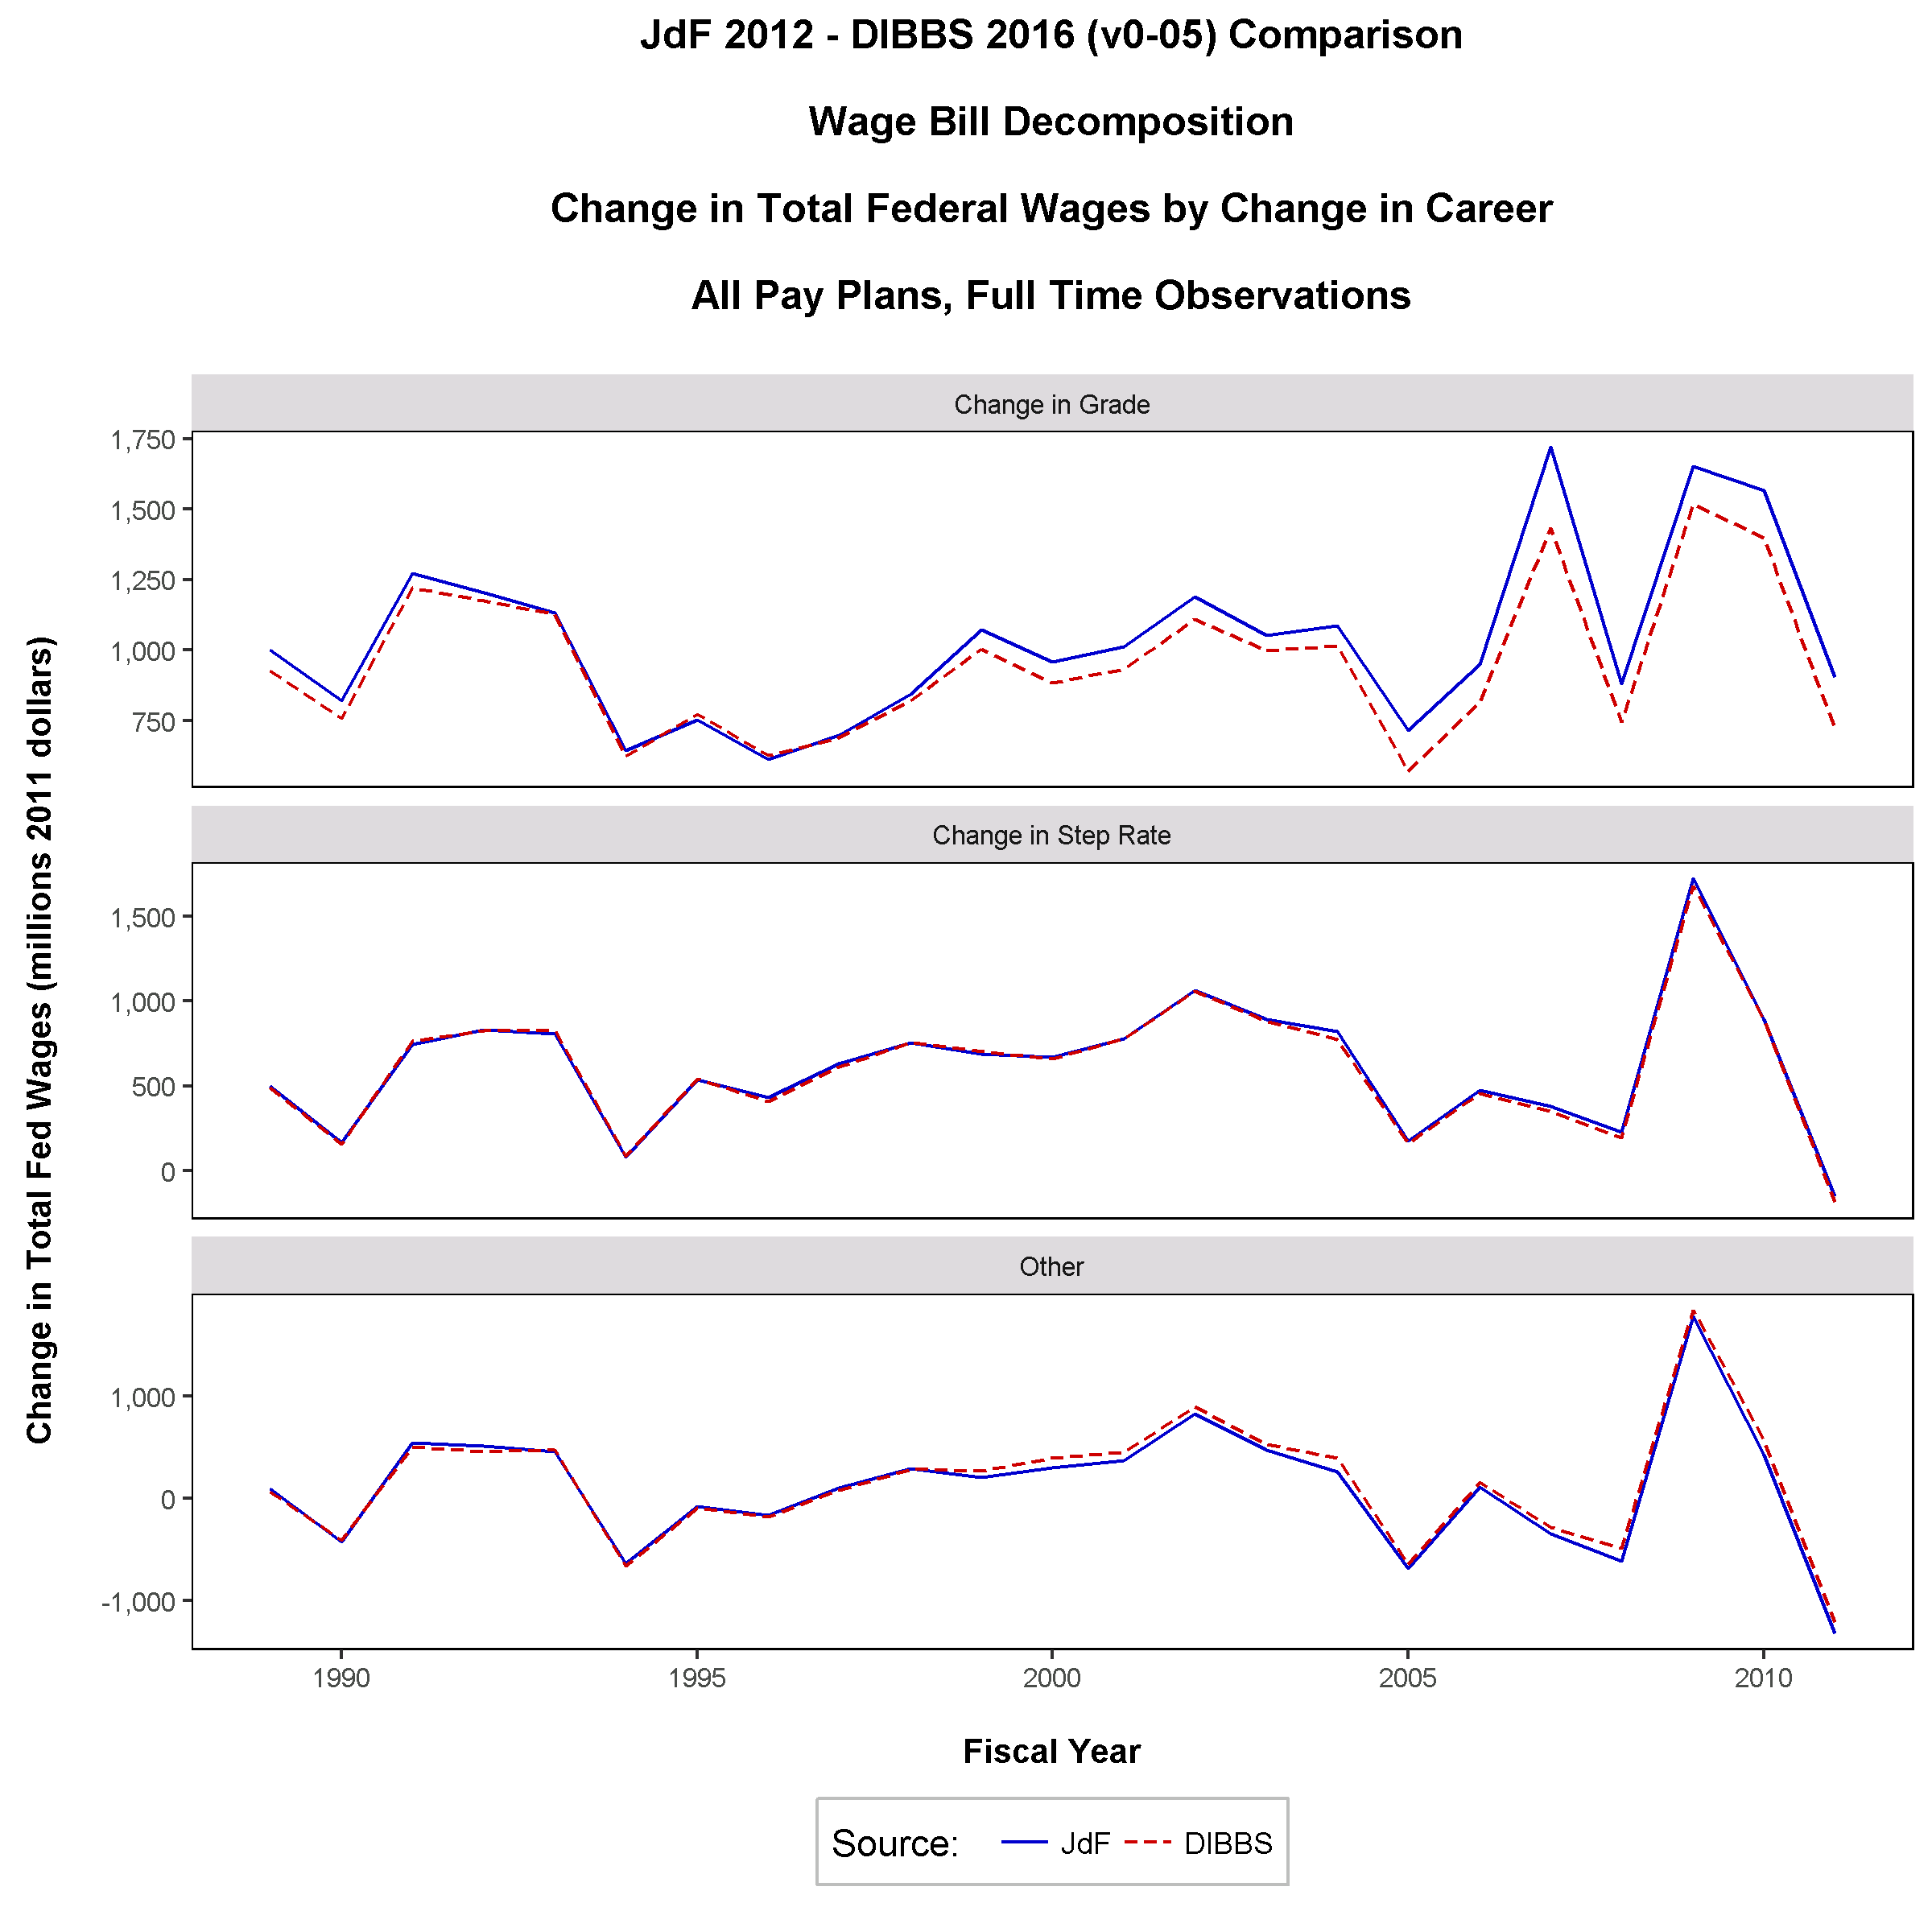
\includegraphics[width=6in, trim={0 0.6in 0 1.5in}, clip]{WageChangePromotionVsFYAllPayPlans.png}
    \caption{Change in U.S. federal government total wage bill.  Millions of 2011 dollars by change in grade, change in step rate, and other changes.  Fiscal years 1988 through 2011. }
    \label{figure:WageChangePromotionVsFYAllPayPlans}
\end{figure}

\clearpage

THE RISE OF GRADE IN THE FED GOVT:  CHANGE IN GS GRADE DISTRIBUTION 2011 vs. 1988\\

The GS pay plan represents approximately 80\% of the observations in the data provided by OPM.  Accordingly, change in distribution of grade within this pay plan is an important consideration when conducting human capital research with these data.  Figure \ref{figure:GSGradeDistribution1988-2011} shows the change in grade distribution from fiscal years 1988 (solid line) to 2011 (dashed line).\\

Observation:  Although highly aggregated, each graph is informative and the synthetic data provide near identical insight into overall change patterns as do the authentic data.\\

\vspace{12pt}

\begin{figure}[h!]
    \centering
    \includegraphics[width=6in, trim={0 0.6in 0 0.6in}, clip]{GSGradeDistribution1988-2011.png}
    \caption{Change in GS grade distribution.  Fiscal years 1988 (solid line) and 2011 (dashed line).  Near identical distribution in synthetic and authentic data.}
    \label{figure:GSGradeDistribution1988-2011}
\end{figure}

\clearpage

THE RISE OF GRADE IN THE FED GOVT:  90/10 PAY PERCENTILE RATIO\\

In addition to a general increase in wages over their study period, Bolton and de Figueiredo show, for the GS pay plan, that wages for employees at the top end increased at a greater rate than for lower paid employees.  Figure \ref{figure:BasicPayQuantile9010Ratio} plots the ratio of 90th and 10th basic pay percentiles for the GS pay plan, grade less than or equal to 15.  Synthetic data are represented by a dashed line, authentic data by a solid line.\\

Observations:  The rise of nearly 0.2 measured in the authentic data is informative and, along with very close tracking of local trends throughout the period, is apparent in the synthetic data.\\

\vspace{12pt}

\begin{figure}[h!]
    \centering
    \includegraphics[width=6in, trim={0 0.6in 0 1in}, clip]{BasicPayQuantile9010Ratio.png}
    \caption{Ratio of 90th and 10th basic pay percentiles by year.  GS pay plan, grade $leq$ 15.  Synthetic data dashed line, authentic data solid.}
    \label{figure:BasicPayQuantile9010Ratio}
\end{figure}

\clearpage

THE RISE OF GRADE IN THE FED GOVT:  BASIC PAY QUANTILE REGRESSION\\

Ordinary least squares regression estimates expected values, given levels of independent, or predictor, variables.  Of interest with distribution of income are quantiles, or an estimate pay below which a given proportion of observations are observed. Figure \ref{figure:BasicPayQuantileYearRegression} plots, for pay plan GS, grade less than or equal to 15, the slopes estimated from the simple linear quantile regression of the logarithm of basic pay on fiscal year (1988-2011).  These slopes represent change in corresponding quantile per year.  One model fit for each quantile from 0.1 through 0.9 in 0.1 increments.  Synthetic data are represented by a dashed line, authentic data by a solid line.\\

Observation:  Similar trends in slope of log(pay) quantile with respect to year are revealed by both data sets.\\

\vspace{12pt}

\begin{figure}[h!]
    \centering
    \includegraphics[width=6in, trim={0 0.6in 0 1in}, clip]{BasicPayQuantileYearRegression.png}
    \caption{Coefficients (change per year) from quantile regression of log(pay) on year.  GS pay plan, grade $\leq$ 15.  1988-2011.  Synthetic data dashed line, authentic data solid.}
    \label{figure:BasicPayQuantileYearRegression}
\end{figure}

\clearpage

THE RISE OF GRADE IN THE FED GOVT:  AGE OF THE FEDERAL EMPLOYEE\\

As a proxy for experience, employee age is an important independent variable in human capital research.  Two aspects of age that Bolton and de Figueiredo measure are change, throughout their study period, in mean age of all employees and in mean age of first year employees.  Figure \ref{figure:AgeVsFYAllPayPlans} plots these means against fiscal year.   Synthetic data are represented by a dashed line, authentic data by a solid line.\\

Observations:  Mean age of all employees and first year employees increases throughout the study period, indicating an increasingly experienced workforce and apparent hiring of employees with increasing levels of experience.  Although actual means of first year age are slightly underestimated in the synthetic data, overall and local authentic trends are accurately represented in the synthetic data.\\

\vspace{12pt}

\begin{figure}[h!]
    \centering
    \includegraphics[width=6in, trim={0 0.6in 0 1in}, clip]{AgeVsFYAllPayPlans.png}
    \caption{Change in mean age of all and first year federal employees.  1988-2011.  Synthetic data dashed line, authentic data solid.  Authentic trends accurately reflected in synthetic data.}
    \label{figure:AgeVsFYAllPayPlans}
\end{figure}

\clearpage

THE RISE OF GRADE IN THE FED GOVT:  EDUCATION LEVEL OF THE FEDERAL EMPLOYEE\\

Employee education is an important independent variable in human capital research.  Two aspects of education that Bolton and de Figueiredo measure are change, throughout their study period, in mean years of education for all employees and for first year employees.  Figure \ref{figure:EdVsFYAllPayPlans} plots these means against fiscal year.   Synthetic data are represented by a dashed line, authentic data by a solid line.\\

Observations:  Mean years of education for all employees and first year employees increases throughout the study period, indicating an increasingly educated workforce.  Although showing slight deviations from authentic annual means, means in the synthetic data accurately represented overall and local trends.  The major reduction in 2002 is attributed to establishment of the Transportation Security Administration.\\

\vspace{12pt}

\begin{figure}[h!]
    \centering
    \includegraphics[width=6in, trim={0 0.6in 0 1in}, clip]{EdVsFYAllPayPlans.png}
    \caption{Change in mean years of education for all and first year federal employees.  1988-2011.  Synthetic data dashed line, authentic data solid.  Authentic trends accurately reflected in synthetic data.}
    \label{figure:EdVsFYAllPayPlans}
\end{figure}

\clearpage

\end{spacing}


\newpage

\begingroup
\begin{spacing}{1.0}
    \raggedright
    \bibliography{DataUtilityBibliography}
\end{spacing}
\endgroup

\end{document}